%justified final
%\documentclass[dissertation,justified,copyright,draftimages,final,numbers,sort&compress,gsmodern]{uothesis}

%right ragged final
%\documentclass[dissertation,copyright,draftimages,final,numbers,sort&compress,gsmodern]{uothesis}

%draftcopy
%\documentclass[dissertation,copyright,draftimages,draftcopy,numbers,sort&compress,gsmodern]{uothesis}

%committeedraft
\documentclass[dissertation,copyright,committeedraft,numbers,sort&compress,gsmodern]{uothesis}

\usepackage[english,UKenglish]{babel}
\usepackage{url}
\usepackage{fullpage}
\usepackage{graphicx}
\usepackage{amssymb}
\usepackage{stackrel}
\usepackage{array}
\usepackage{amsmath}
\usepackage{verbatim}
\usepackage{multirow}
\usepackage{rotating}
\usepackage{fancybox}
\usepackage{pdflscape}
\usepackage{amsthm}
\usepackage{blkarray}
\usepackage{algorithmic}
\usepackage{algorithm}

%\input{custom_cmds.tex}

\theoremstyle{definition}
\newtheorem{myexp}{Example}[section]
\theoremstyle{definition}
\newtheorem{mydef}{Definition}[section]
\newtheorem{mythm}{Theorem}[section]
\newtheorem{mylem}{Lemma}[section]
\renewcommand{\algorithmicrequire}{\textbf{Input:}}
\renewcommand{\algorithmicensure}{\textbf{Output:}}
\newcommand\T{\rule{0pt}{2.6ex}}
\newcommand\B{\rule[-1.2ex]{0pt}{0pt}}
\DeclareMathOperator*{\argmin}{arg\,min}
\DeclareMathOperator*{\argmax}{arg\,max}
%THESIS FRONT MATTER

%TITLES.
\covertitle{A Graph-based Approach For \\Semantic Data Mining}
\abstracttitle{A Graph-based Approach For Semantic Data Mining}

%AUTHOR
\author{Haishan Liu}

%DEPARTMENT
\narrowdepartment{Dept. of Computer and Information Science}

\department{Department of Computer and Information Science}

%DEGREE INFORMATION
\degreetype{Doctor of Philosophy}
\degreemonth{June}
\degreeyear{2012}

%COMMITTEE INFORMATION
\advisor{Dr. Dejing Dou}
\chair{Dr. Dejing Dou}
\committee{Dr. Arthur Farley & Inside\\
    Dr. Allen Malony & Inside\\
    Dr. Daniel Lowd & Inside\\
    Dr. Don Tucker & Ouside\\
    %Don Tucker & Honorary\\
}
\graddean{Richard Linton}

%CURRICULUM VITAE
\birthplace{Shanghai}
\birthday{October 12th 1983}

\school{University of Oregon, Eugene, OR}
\school{Shanghai Jiao Tong University, Shanghai, China}

\degree{Master of Science in Computer Science, 2008,
University of Oregon}
\degree{Bachelor of Information Security, 2006,
Shanghai Jiao Tong University.}
\interests{Data mining, machine learning, the Semantic Web}

%\position{Graduate Research \& Teaching Assistant, Department of Computer and Information Science, University of Oregon, 2006 to present}
%\position{Research and Development Intern, Pengyue Technology, Shanghai, 2006}

\award{Graduate Teaching \& Research Fellowship, Computer and Information Science, 2006 to present}
\award{NSF Travel Grant, International Semantic Web Conference, 2010}
\award{NSF Travel Grant, International Conference on Data Mining, 2011}

\publication{Haishan Liu, Paea LePendu, Ruoming Jin, and Dejing Dou. A Hypergraph-based Method for Discovering Semantically Associated Itemsets. In Proceedings of the 11th IEEE International Conference on Data Mining (ICDM), 2011.}

\publication{Haishan Liu and Dejing Dou. Breaking the Deadlock: Simultaneously Discovering Attribute Matching and Cluster Matching with Multi-Objective Simulated Annealing. In Proceedings of the International Conference on Ontologies, Databases and Application of Semantics (ODBASE), pages 698--715, 2011.}

\publication{Dejing Dou, Han Qin, and Haishan Liu. Semantic Translation for Rule-based Knowledge in Data Mining. In Proceedings of the 22nd International Conference on Database and Expert Systems Applications (DEXA), part II, pages 74--89, 2011.}

\publication{Haishan Liu. Towards Semantic Data Mining. In: Doctoral Consortium of the 9th International Semantic Web Conference (ISWC), November 2010.}

\publication{Christopher Townsend, Jingshan Huang, Dejing Dou, Shivraj Dalvi, Patrick J. Hayes, Lei He, Wen-chang Lin, Haishan Liu, Robert Rudnick and Hardik Shah. OMIT: Domain Ontology and Knowledge Acquisition in MicroRNA Target Prediction. On-The-Move Conferences 2010 (OTM): 1160--1167}

\publication{Haishan Liu, Gwen Frishkoff, Robert Frank, and Dejing Dou. Ontology-based Mining of Brainwaves: A Sequence Similarity Technique for Mapping Alternative Descriptions of Patterns in Event Related Potentials (ERP) Data. In Proceedings of the 14th Pacific-Asia Conference on Knowledge Discovery and Data Mining (PAKDD), pages 43--54, 2010.}

\publication{Gwen Frishkoff, Paea LePendu, Robert Frank, Haishan Liu, and Dejing Dou. Development of Neural Electromagnetic Ontologies (NEMO): Ontology-based Tools for Representation and Integration of Event-related Brain Potentials. In Proceedings of the International Conference on Biomedical Ontology (ICBO), pages 31--34, 2009.}

%\publication{Haishan Liu, Gwen Frishkoff, Robert Frank and Dejing Dou. Mapping ERP patterns from heterogeneous datasets: A simulation study. Poster in the 15th Annual Meeting of the Organization for Human Brain Mapping (HBM). June, 2009.}

\publication{Haishan Liu and Dejing Dou. An Exploration of Understanding Heterogeneity through Data Mining. In Proceedings of KDD'08 Workshop on Mining Multiple Information Sources, pages 18--25, 2008.}

\publication{Jongwan Kim, Dejing Dou, Haishan Liu, and Donghwi Kwak. Constructing a user preference ontology for anti-spam mail systems. In Proceedings of the 20th Canadian Conference on Artificial Intelligence (Canadian AI), pages 272--283, 2007.} 

%ACKNOWLEDGEMENTS
\acknowledge{Toward my many mentors I feel the deepest gratitude and respect. In particular, I acknowledge the tireless support of my research advisor, Dr. Dejing Dou, who provided guidance to me through all the steps that led to this dissertation. I also sincerely thank the Computer and Information Science (CIS) faculty, staff and my committee members for their time, encouragement, instruction and support.  I have fond remembrances of my assistantships on the Neural ElectroMagnetic Ontologies (NEMO) projects and I thank those colleagues for wonderful experiences.

I humbly acknowledge the funding support of the CIS department, Dr. Dejing Dou, and NEMO during my studies.

I would like to finally thank my parents and family for giving me the opportunity to fulfil my dreams and support to achieve my ambitions. Without them this work would not have been concluded.}

%Looks good.  My recommendation is that you do name Dejing in the last sentence and that you change "everything in general" to something more like "their time, encouragement, instruction and support" in the second sentence.  Then delete "specifically" at the end of the second sentence. 

%DEDICATION (optional)
\dedication{This work is dedicated to my wife Xiaofei Zhang for her support and endurance in all those moonlight nights we are apart.} 

%ABSTRACT
\abstract{Data mining, also referred to as knowledge discovery in databases (KDD), is the nontrivial extraction of implicit, previously unknown, and potentially useful information from data. The measure of what is meant by ``useful" to the user is dependent on the user as well as the domain within which the data mining system is being used. Therefore, the role of domain knowledge in the discovery process is essential. However, previous research has made limited attempts to build data mining systems that are capable of incorporating domain knowledge in a principled manner. This motivates us to develop a framework for explicit incorporation of domain knowledge in a data mining system so that insights can be drawn from both knowledge and data in a systematic way. We call such technology the semantic data mining.

Latest research in knowledge representation, particularly in the area of W3C's Semantic Web that seeks to embed semantic content in web pages, has led to mature standards such as the Web Ontology Language (OWL) for authoring ontologies. An ontology is an explicit specification of a conceptualization. Today, Semantic Web ontologies have become a key technology for intelligent knowledge processing, providing a framework for sharing conceptual models about a domain. We make extensive use of ontologies as a means encode domain knowledge in this dissertation.

The OWL ontology language is built on the W3C's Resource Description Framework (RDF) that provides a simple model to describe information resources as a graph. At the same time, there has been a surge of interest in tackling the problem of mining semantically rich datasets, where objects are linked in a number of ways. In fact, many datasets of interest today are best described as a linked collection, or a graph, of interrelated objects. It can be seen that, the interface between domain knowledge and data mining can be possibly achieved by using graph representations in which distinct sorts of knowledge that has been traditionally differently represented can be structured in a unified manner. Therefore, in this dissertation, we explore a graph-based approach for modeling both knowledge and data, and for analyzing the combined information source from which insight can be drawn systematically.

This dissertation presents two novel directions in semantic data mining. First, we describe how a graph interface for both knowledge representation and data mining can be structured. This is achieved by employing the RDF model and by the fact that RDF allows a combined specification of both schema and data structured under this schema. We propose to use the RDF hypergraph (bipartite) model as the unified representation for both data and domain knowledge. And second, we describe a graph theoretic analysis approach for mining the combined information source of both data and knowledge. We showcase hypergraph-based analysis method for an important data mining task, namely, the frequent pattern mining. We hope these novel contributions can lead to the development of new principles towards semantic data mining.} 

%Main Document
\begin{document}
\maketitle

%CHAPTERS
\chapter{INTRODUCTION}
\label{chap:introduction}
%\cite{LiuEtal11}\cite{LiuDou11}\cite{DouEtal11}\cite{liu2010}\cite{LiuEtal10}\cite{FrishkoffEtal09}\cite{LiuDou08}\cite{KimEtal07}


%In a rough sense, such links between objects can be viewed as foreign keys in relational databases. To this end, mining Semantic Web data is somewhat analogous to multi-relational data mining (MRDM). However the sheer number of links and the scale of data would render MRDM techniques impractical for most uses (e.g., the DBpedia dataset). We hope to develop native graph based approach for data mining that is able to effectively and efficiently utilize rich information in Semantic Web datasets such as RDF and OWL.
Data mining, also referred to as knowledge discovery in databases (KDD), is the nontrivial extraction of implicit, previously unknown, and potentially useful information from data~\cite{Frawley1992}. But the measure of what is meant by ``useful" to the user is dependent on the user as well as the domain within which the data mining system is being used. Therefore, the role of domain knowledge in the discovery process is essential. Fayyad \etal~\cite{Fayyad96} contended that the use of domain knowledge is important in all stages of the data mining process including, for example, data transformation, feature reduction, algorithm selection, post-processing, model interpretation and so forth.

The first step towards using domain knowledge is to acquire the knowledge from experts and thus model and codify the knowledge in computer. Russell and Norvig~\cite{Russell03} emphasized that a data mining system must have some method for obtaining the background knowledge and can no longer make naive speculations, and should use its background knowledge to learn more and more effectively. this process of modeling knowledge in computer systems to facilitate problem solving is studied in the field of knowledge representation/engineering. Research in this field has resulted in many sophisticated technologies such as expert system. However, at present, knowledge representation and data mining remain largely separate disciplines. Although it is widely stated that exploring the fusion of the two fields is worthwhile in many applications where substantial human expertise exists alongside data resources, as many researchers have pointed out, work along this line is still in its infancy~\cite{Hirsh94, Weiss01, Daniels01, Kopanas02, Langseth03}.

Previous research has made limited attempts to build data mining systems that are capable of incorporating domain knowledge in a principled manner. In those systems where users are allowed to express domain knowledge, such knowledge is often specified in a very application-specific form, scope and granularity. The ad hoc manner of representing knowledge hinders the interoperability and reuse of codified knowledge~\cite{Pohle03}. Moreover, we have also observed that in many data mining systems, domain knowledge is embedded into the implementations in the form of implicit assumptions and heuristics, which makes abstraction and refactoring particularly hard. Sometimes even data mining practitioners themselves are not aware of employing domain knowledge in such a manner. This motivates us to develop a framework for explicit incorporation of domain knowledge in a data mining system so that insights can be drawn from both knowledge and data in a systematic and holistic way. We call such technology the ``semantic data mining''.

Latest research in knowledge representation, particularly in the area of W3C's Semantic Web~\cite{Berners-Lee01} that seeks to embed semantic content in web pages, has led to mature standards such as the Web Ontology Language (OWL~\cite{OWL}) for authoring ontologies. An ontology is an explicit specification of a conceptualization~\cite{Gruber93}. Today, Semantic Web ontologies have become a key technology for intelligent knowledge processing, providing a framework for sharing conceptual models about a domain~\cite{Maedche03Onto}. Ontologies explicate domain knowledge hence providing a way to separate knowledge from implementations~\cite{Noy01ontologydevelopment}. Much effort has been devoted to developing tools for coding and managing OWL ontologies~\cite{Duineveld00, Knublauch04}. Many of the technologies proposed by the W3C already existed before they were positioned under the W3C standards and recommendations. Ontologies are used in various contexts, particularly those dealing with information that encompasses a limited and defined domain, and where sharing data is a common necessity, such as scientific research. Prominent examples of such efforts include the Gene Ontology (GO~\cite{GO}), Unified Medical Language System (UMLS~\cite{UMLS}), and more than 300 ontologies in NCBO (National Center for Biomedical Ontology) such as the Neural ElectroMagnetic Ontologies (NEMO~\cite{FrishkoffEtal07, FrishkoffEtal09}).

%\here These technologies are combined in order to provide descriptions that supplement or replace the content of Web documents. Thus, content may manifest itself as descriptive data stored in Web-accessible databases,[13] or as markup within documents (particularly, in Extensible HTML (XHTML) interspersed with XML, or, more often, purely in XML, with layout or rendering cues stored separately). The machine-readable descriptions enable content managers to add meaning to the content, i.e., to describe the structure of the knowledge we have about that content. In this way, a machine can process knowledge itself, instead of text, using processes similar to human deductive reasoning and inference, thereby obtaining more meaningful results and helping computers to perform automated information gathering and research.

%\here From a modeling viewpoint, we see two essential properties in the basic conceptual graph model. The objects. i.e., basic graphs. are easily understandable by users (typically knowledge engineers or specialists in an application domain), at least if the graphs are reasonably small (note that it is always possible to split up a large conceptual graph into smaller ones while keeping its semantics). This feature partially explains the success of semantic networks and, more generally, the success of graphical models, such as the entity/relationships model, UML, Topic Maps, etc. Many people. and not only computer scientists, are now familiar with kinds or labeled graphs (mainly trees, but not exclusively). This fact is especially important in knowledge acquisition. In our approach to CGs, this quality does no only concern the descriptive facet of the formalism. Reasoning mechanisms are also easily understandable, for two reasons. First, homomorphism is a ``global" graph--matching notion that can he easily visualized (we will also see that homomorphism is equivalent to a sequence of elementary graph operations which are very simple and easy to visualize). Secondly, the same language is used at interface and computing levels. In particular, no transformation has to be done on the components of the knowledge base before reasoning with it.

%\here As already said, in order to understand the results given by the system, a precise description of what is obtained (a denotational semantics) is mandatory. However, in some situations. especially whenever the knowledge deals with a poorly formalized application domain, it may be useful to understand how the results have been obtained. i.e.. to have an operational semantics. This point is important because there can he a gap between the program and the knowledge represented in the system, i.e., a formal system, and the knowledge itself. There should he a tight correspondence between what is seen by the user and how objects and operations are implemented. This correspondence should be tight enough to enable faithful modeling of the actual data and problems, and to understand why and how results have been obtained. A way t0 limit the semantic gap is to use a homogeneous model---the same kinds or object and the same kinds of operation occur at each fundamental level (formal. user interface, implementation). Such a correspondence is sometimes called an ``isomorphism," but this designation can be misleading. Indeed, this correspondence is not a mathematical function between two mathematical objects but is rather a correspondence between ``reality" and a mathematical object. There is a gap between a reality and the concepts describing it. as well as between a conceptual modeling and its implementation. i.e.. a representation of this modeling by computational objects. Moreover, as in this book we use ``isomorphism" in its usual mathematical sense, we avoid using it metaphorically.

The OWL ontology language is built on the W3C's Resource Description Framework (RDF) that provides a simple model to describe information resources as a graph. The core of the framework is the RDF statements consisting of triples including a subject (the resource being described), a predicate (the property) and an object (the property value). This simple model of assertions leads to a network of information resources, interrelated by properties which establish relations, or links, between resources and property values. The term RDF Graph is defined as a set of RDF triples (which can be illustrated by a node-arc-node link). Therefore, any collection of RDF data is an RDF Graph~\cite{GraphModelRDF}.

At the same time, there has been a surge of interest in tackling the problem of mining semantically rich datasets, where objects are linked in a number of ways. In fact, many datasets of interest today are best described as a linked collection, or a graph, of interrelated objects~\cite{LinkMiningGetoor}. These graphs may represent homogeneous networks, in which there is a single-object type and link type (such as web pages connected by hyperlinks), or richer, heterogeneous networks, in which there may be multiple object and link types (such as DBpedia, a data source containing structuralized information from Wikipedia). Many traditional information resource and format can be viewed as graphs or linked collections as well. Such links and their characteristics are explored, often implicitly, by those well established data analysis and mining techniques, whose formalism of the problem are however typically not based on graphs. For example, consider a simple transaction table and the problem of frequent itemset generation. An itemset is deemed frequent if its \emph{support}, i.e., the percentage of transactions which contain that itemset, is above a threshold. If we characterize the ``co-occurrence" relationship (items appearing together in a tuple) as a link between items, then the transaction table can be viewed as a graph consisting a set of items connected by such links. Furthermore, in this sense, the problem of frequent pattern mining can be reformulated as to identify sets of nodes in the graph that are heavily connected by the co-occurrence link. %The support of a pattern is a measure of endorsement among items via the co-occurrence link.

It can be seen that, the interface between domain knowledge and data mining can be possibly achieved by using graph representations in which distinct sorts of knowledge that has been traditionally differently represented can be structured in a unified manner. For example, previously, one important aspect of the distinction between domain knowledge and data is the different representations for \emph{ontological} and \emph{factual} knowledge. Ontological knowledge is related to general categories, also called concepts or classes (such as those defined in OWL ontologies). Factual knowledge makes assertions about a specific situation (\eg, ``this specific entity belongs to a certain category. and has a certain relationship with another entity, such as those defined in knowledge bases or relational databases). However, this distinction can be obscured by the simple semantics of the RDF model given the fact that RDF allows a combined specification of both schema and data structured under this schema. Since RDF's abstract triple syntax has a graph nature, and graph is one of the most fundamental objects studied in mathematics that has a strong relation with logical languages and data structures, developing graph-based approach becomes promising for providing a common ground to interface with both domain knowledge and data mining. Therefore, in this dissertation, we explore a graph-based approach for modeling both knowledge and data, and for analyzing the combined information source from which insight can be derived systematically. We expect this novel paradigm to contribute to the development of new principles towards semantic data mining.

%\here Another kind of knowledge is implicit knowledge described. for instance. by rules of form ``if this then that" (e.g.. ``if there is a relation r from x to v, then the same relation r also holds from y to x"). Different kinds of rules can be considered. Some rules can be included in an ontology (e.g.. the transitivity of a binary relation), other rules, for instance representing possible transformations, are not ontological knowledge. Constraints, i.e., conditions that are to he fulfilled by some pieces of knowledge in order to be correctly processed by a reasoning engine, frequently appear in modeling and should be differentiated from other kinds of knowledge.


Since graph-based semantic data mining is a new field, many interesting research directions related to it are yet to be explored. This dissertation studies two such research directions, which have the potential to make significant contributions towards improving the data mining systems carried out by systematically incorporating domain knowledge. Brief description on these two directions are presented below.

\begin{enumerate}
\item \textbf{A graph representation for both domain knowledge and data mining.}
    The interface between knowledge representation and data mining is achieved by employing the RDF model and by the fact that RDF allows a combined specification of both schema and data structured under this schema.

    RDF's ability to represent disparate, abstract concepts has led to its increasing use in knowledge representation. To express schematic information, RDF by itself provides only the most basic predefined concepts, the so-called RDF core vocabulary and RDF Schema. RDF Schema permits elementary structuring of a vocabulary, which enables a type-focused understanding of a vocabulary for machine agents %and can support ``semantic" querying at a first stage
    ~\cite{GraphModelRDF}. However, RDF Schema's expressiveness is limited to basic assertions about class and property relationships. ``Richer" schema and ontology defining languages (e.g., OWL) that are built upon RDF continue to evolve. %Its limited expressivity, however, falls short of what shall be provided by true ontology specification languages such as OWL~\cite{OWL}.

    On the other hand, in practice, vast amount of data is often persisted in relational databases (RDB). Mapping from RDB to RDF has gained increasing attention and led to implementation of generic mapping tools as well as domain--specific applications.  The W3C launched the RDB2RDF incubator group to explore issues involved in mapping RDB to RDF. A work-in-progress survey paper has been published documenting approaches in this field~\cite{RDB2RDF}.

    An outstanding advantage of expressing data in RDF is the explicit modeling of relationships between entities that are either implicit or non--existent in RDB. And in such way, one can achieve the incorporation of ``domain semantics", an important aspect to fully leverage the expressivity of RDF models that enables data mining systems to explore beyond pure data. Furthermore, the role of RDF as an integration platform for data from multiple sources is another main motivations for mapping RDB to RDF.

    RDF's abstract triple syntax has a graph nature. Graphs are mathematical objects that enjoy wide-spread usage for many tasks, which include the visualization and analysis of data for humans, mathematical reasoning, and the implementation as a data structure for developing data mining algorithms. Besides the common graph-theoretic model of RDF as labeled, directed multi-graphs, Hayes has established that RDF can be also represented as hypergraphs (bipartite graphs)~\cite{GraphModelRDF}. This result constitutes an important aspect of the theoretical basis of this dissertation and is discussed in the Background Chapter. We have also developed various ways to represent data for different data mining tasks, including association rule mining, classification, clustering and so forth, details of which shall be described in Chapter III and IV.

\item \textbf{A graph theoretic analysis approach for mining the combined information source of both data and knowledge.}

    Using graph-based formalisms can bring new perspectives to traditional data mining tasks. For example, as mentioned before, the problem of frequent pattern mining can be reformulated as to identify sets of nodes in the graph that are heavily connected by the co-occurrence link. It is evident that the traditional measure of support is essentially restrained to only take into account direct links between items while ignoring the indirect ones (those through intermediaries). A prominent example of such indirect association was given by Swanson's land mark paper published in 1987~\cite{swanson87} before the age of Web-scale computation:
    Let A stand for dietary fish oil; let B stand for a set of certain changes in the blood and circulatory system; and let C stand for the amelioration of Raynaud's syndrome, a peripheral circulatory disorder. Swanson was the first to hypothesize that dietary fish oil might benefit people afflicted with Raynaud's syndrome (A is associated with C) given that it had been already widely known that dietary fish oil causes certain blood changes (A is associated with B) and that these same blood changes may ameliorate Raynaud's syndrome (B is associated with C). The latter two associations were supported by substantial bodies of evidence but were mutually isolated and apparently had never been brought together in print. Without discovering that indirect association (A and C) a potentially useful hypothesis that is worth testing would have been missed. A graph-based analysis approach is particularly suitable to effectively discover this kind of pattern.

    In the context of a graph model for RDF, it is useful to introduce some kind of distance metric between information resources to approach the intuitive notion of relatedness between resources. The relation between resources is founded on the paths which connect them. Simply taking the path length as a distance metric would be a naive approach. More sophisticated metric may consider spectral information of the graph or employ weighting schemes to account for meaning of the connecting properties (edges). With a reasonable graph model as well as a meaningful distance metric defined, a lot of traditional mining problems, including frequent pattern mining, clustering and classification, can be tackled in a new angle with the ability to tap on domain knowledge expressed in the same graph model.

    At the same time, we note that these problems may be more challenging in the graph domain which is due to the cost of the greater expressive power associated with graphs. In addition, different mining tasks and applications require different kinds of graphs and face varied corresponding challenges. For example, some data graphs are relatively small but involve a large number of semantic types resulting in highly heterogeneous connection. On the other hand, in many large scale domains such as the web and social networks, the node labels (\eg. URLs) are distinct, but the number of nodes is overwhelming. Such graphs are also challenging because the degree distributions of these graphs are highly skewed~\cite{Faloutsos1999}. Drawing inspiration from a broad body of literature on graph mining and graph spectral analysis, we aim at developing effective and efficient graph theoretic analysis methods for mining the unified graph representation modeling information in both domain knowledge and data.

\end{enumerate}

The remainder of this dissertation is organized as follows. In Chapter II, we discuss the background areas related to the original research work presented. The main contributions of this dissertation are presented in Chapters III, IV, V and VI. Chapters III discusses the theory of hypergraph-based representation of both knowledge and data. Chapter IV introduces the notion of semantic annotation and proposes a mining-based approach as well as a method for integration in the scenario where multiple ontologies or meta-data definitions are presented. Chapters V is dedicated to the hypergraph-based analysis method on the combined information source of both knowledge and data graph for traditional data mining tasks with a focus on frequent pattern mining. Chapter VI demonstrates implementation and case studies. Finally, in Chapter VII, we discuss future directions for the research work and provide some concluding remarks.



%The formalism is based on graphs and graph-theoretic notions and operations. It is logically founded, but in some way is ``autonomous"  from (existing) logics. Stated differently, our KR formalism is a pure graph-theoretic formalism, whose core corresponds to a FOL fragment, and most extensions of this core correspond to FOL fragments. Since it is embedded in graph theory, it is easy to define new operations, simple from a graph viewpoint, and having simple intuitive semantics, but that do not necessarily have a formal semantics expressed in a classical logic.



%The underlying structure of any expression in RDF is a collection of triples, each consisting of a subject, a predicate and an object. A set of such triples is called an RDF graph. This can be illustrated by a node and directed-arc diagram, in which each triple is represented as a node-arc-node link (hence the term ``graph").




%Each of these reasons plays an important role in facilitating synergy between domain knowledge and data mining. As mentioned above, we have observed that without a standard language bearing unified semantics, such as Semantic Web ontologies, domain knowledge tends to be woven into implementation of data mining techniques in an ad hoc way. Sometimes even practitioners themselves are not aware of doing so. Therefore, we propose to exploit the advances of Semantic Web ontologies to formally represent domain knowledge including structured collection of prior information and set of inference rules, and thus develop frameworks for incorporation of domain knowledge in an intelligent data mining environment. We call such technology the semantic data mining.

%This paper focuses on three areas of research in the field of semantic data mining. It aims at summarizing representative academic work featuring the state-of-the-art, innovative theoretical frameworks, advanced implementations as well as latest empirical research findings that are critical to realizing the semantic data mining. The areas are described below:
%\begin{itemize}
%\item Domain knowledge driven data mining, a term we use to give a single collective name for researches on combining domain knowledge and data mining. We survey a body of work on this topic and compile a list of classification schemes that have been proposed to specify categories of domain knowledge. We believe a proper classification provides a framework useful for characterizing a wide variety of systems and reveals essential similarities and differences.
%\item Semantic Web: We briefly introduce history and current status of the Semantic Web, with a focus on its structure, current proposals for standard languages, and future direction. We also examine reasons why the Semantic Web is a competent approach for incorporating domain knowledge in data mining.
%\item Semantic data mining, a new field we envision emerging, where data mining is strengthened with the latest Semantic Web technologies. We introduce some pioneering work in this field that enhances the data mining process by taking advantage of ontologies. We also survey a growing line of research focusing on semantic annotation that aims at bringing meaning into data.
%\end{itemize}
%The rest of the paper is organized as follows: we survey the research in combining domain knowledge with data mining in section 2. In section 3, we present a brief introduction of the structure and vision of Semantic Web. In section 4, we survey a body of research that uses ontology as a way to formally represent knowledge and incorporate such representation in data mining. We also examine the field of semantic annotation. Section 5 concludes the paper and presents a list of future directions.







%A machine-understandable mechanism for the definition of vocabularies is of crucial importance so that a Semantic Web attains the same degree of technical interoperability and growth-ensuring extensibility as the World Wide Web showed in the past.

%RDF provides the ``skeleton" for making assertions, but not the ``flesh": the meaning of an RDF expression depends on the understanding of the concepts that the RDF statements are made up of. RDF by itself provides only the most basic predefined concepts, the so-called RDF core vocabulary, and RDF Schema. RDF Schema permits elementary structuring of a vocabulary, which enables a type-focused understanding of a vocabulary for machine agents and can support ``semantic" querying at a first stage~\cite{GraphModelRDF}. Its limited expressivity, however, falls short of what shall be provided by true ontology specification languages such as OWL~\cite{OWL}. RDF and OWL constitute the building blocks of the Semantic Web~\cite{SemanticWebRoadmap}. The Semantic Web is the vision of a machine-understandable (understandable as a contrast to the contemporary machine-processable content) web of information resources. This means that resources as well as relations between resources are characterized in a formal way. The Semantic Web has been extensively harnessed in scientific areas especially in biology and biomedical engineering. knowledge is evolving so rapidly in those fields and promoting the creation and use of ontologies for the field and linking to other ontologies in related domains holds the promise of making more rapid scientific progress. Prominent examples of this effort include the Gene Ontology (GO~\cite{GO}), Unified Medical Language System (UMLS~\cite{UMLS}), and Neural ElectroMagnetic Ontologies (NEMO~\cite{FrishkoffEtal07, FrishkoffEtal09}).



%Suppose given a relation table of annotated medical publications in a ``bag-of-word" representation where each row corresponding to one publication and each column a boolean variable indicating if some term is appeared. Using traditional frequent itemset generation algorithms, if the number of times the item pair \emph{fish oil} and \emph{Raynaud's syndrome} occurring together falls below some threshold, then $\langle$\emph{fish oil}, \emph{Raynaud's syndrome}$\rangle$ would not be picked up as a frequent itemset. However \emph{fish oil} and \emph{Raynaud's syndrome} may actually be meaningfully related and the latent association can be revealed through indirect links. For instance, if $\langle$\emph{blood changes}, \emph{fish oil}$\rangle$ and $\langle$\emph{blood changes}, \emph{Raynaud's syndrome}$\rangle$ are both frequent, the presence of \emph{blood changes} provides a connection through which \emph{fish oil} and \emph{Raynaud's syndrome} can be related (this relationship is discovered in Swanson's land mark paper published in 1987~\cite{swanson87} before the age of Web-scale computation). We call the intermediary item such as \emph{blood changes} in this case a \emph{linking item}, and the latent association between two items through the connection via one or more linking items the \emph{semantically associated relationship}. We propose that new data mining methods depending on graph/link-based formalism are best suitable for discovering this kind of pattern.

%RDF possesses a graph nature which allows information of data and meta-data to be described in the same framework. This characteristic is critical in enabling the synergy between domain knowledge and data mining. Inspired by this, the central thesis of the paper is a proposal to develop a \emph{semantic data mining} framework by using graph-based representation and analysis methods in order to achieve the systematic incorporation of semantics of domain knowledge in data mining. 

%%%%%%%%%%%%%%%%%%%%%%%%%%%%%%%%%%%%%%%%%%%%%%%%%%%%%%%%%%%%%%%%%%%

\chapter{BACKGROUND}
\label{chap:background}
This chapter covers the background areas and related work necessary to understand the contributions of this dissertation. It discusses the current state of the effort to incorporate domain knowledge in data mining. In addition, it describes the various formalisms proposed in the literature to use graphs in tackling data mining and knowledge representation problems. We conclude with a high-level summary of these background areas.

\section{Domain Knowledge in Data Mining}
Domain knowledge relates to information about a specific domain or data that is collected from previous systems or documentation, or elicited from domain experts. In the rest of the section, we highlight a body of studies that aims at exploring ways to employ domain knowledge in data mining. The results from these studies strongly attest to the positive influence of domain knowledge. Domain knowledge can affect the discovery process within a data mining system in at least two ways. First, it can make patterns more visible by generalizing the attribute values, and second, it can constrain the search space as well as the rule space.

In order to effectively summarize and compare different previously proposed systems, we propose a reference framework to classify different kinds of domain knowledge at a very high abstraction level as detailed in the following.

\begin{itemize}
\item	Knowledge about the domain: This category contains information related to a specific domain of discourse, usually obtained from either domain experts or previous data mining processes. Examples of such knowledge include concept hierarchy, integrity constraints, \etc.
\item	Knowledge about the data: This category contains information about dataset, including how it is generated, transformed and evolved. This knowledge is obtained from data producers (people who carry out experiments or collect data) or database managers. \eg, in a database of spatial information, one of the images may have been recorded with a very skew angle on the object. When processing the database the discovery process must take this information into account.
\item	Knowledge about the data mining process: This category contains information pertaining to specific data mining sessions, including goals, parameters and variables related to the experiment. \eg, attributes of interest within data, roles of attributes as being whether antecedents or consequences in association rule mining, and the measure of interestingness for discovered patterns.
\end{itemize}

The summarized work can be divided into two groups. The first group does not explicitly leverage any knowledge representation approaches to model domain knowledge. The second group explores mainly ontological knowledge (concept hierarchy) and uses formal ontology languages to encode such knowledge. The kind of domain knowledge involved in the first group is broader which covers all categories discussed in the above reference classification scheme. However, it is achieved at the cost of less formality which often result in ad-hoc expression of domain knowledge that has a very application-specific form, scop and granularity.

%Various studies have shown that employing domain knowledge can benefit data mining in a number of ways. Sinha et al. [18] postulated that infusing domain knowledge would reduce the hypothesis space, thereby facilitating search for a solution. Yoon et al. [26] described a similar idea and provided several illustrative motivating examples. They demonstrated that domain knowledge can be used to reduce the size of the database by eliminating data records or irrelevant attributes that are not needed for discovery or by refining the original query via posing more restrictions. In other words, with domain knowledge, data mining queries can be transformed into forms that are more efficiently processable.

%Daniels et al. observed difficulties when applying models derived from data mining processes without considering domain knowledge [11]: i) Incompatibility of mined model and domain knowledge, ii) lack of interpretability of the model. Quite often it is more important to gain insight in the decision problem than to have accurate predictions. And iii) knowledge representation at the wrong level of detail. Data mining algorithms often yield structures or models that are intractable for human decision makers due to their huge complexity. They further claimed that, in a variety of business intelligence applications, domain knowledge would improve the efficiency of data mining systems: i) Risk assessment in the presence of both qualitative knowledge and legal or contractual constraints. ii) Classification and description of customer groups in evaluation decision processes such as credit loan evaluation and fraud detection. iii) Validation of business rules especially in distributed user environments. And iv) all kinds of price models for trend analysis or automatic trading employed in combination with transaction databases.

%Despite that the benefits abound, it is known that there still has been little research focusing on the combination of domain knowledge and data to date. Sinha et al. [18] elaborated that the reason of the lack of attention to the role of domain knowledge in data mining research partly attribute to the fact that domains of application are typically data-rich, giving the impression that domain knowledge is not really necessary. Also, the fact that in many domains expert knowledge is not readily available or, even when available, knowledge acquisition tends to be a difficult and time-consuming process, could be a factor in not addressing the issue of domain knowledge.

%We end this section by providing a summary of the ontology-based data mining systems discussed throughout this section. Table 1 shows how they are classified on the dimensions we have discussed.

In one of the earliest studies on the subject, Pazzani and Kibler~\cite{Pazzani1992} developed a general purpose relational learning algorithm called FOCL, which combines explanation-based and inductive learning. In a later study, they conducted an experiment comparing FOCL with a domain theory to FOCL without a domain theory. A partial knowledge base of an expert system was used as the domain theory. They found that incorporating domain theory significantly reduced misclassification costs when larger training sets were used.

In another study, Ambrosino and Buchanan~\cite{Ambrosino1999} examined the effects of adding domain knowledge to a rule induction program for predicting the risk of mortality in patients with community--acquired pneumonia. They developed a graphical data exploration tool for domain experts to encode domain knowledge and interact with the data mining process. The domain experts participated in two stages of mining. They were first asked to modify the existing set of attributes according to their domain knowledge, and then they were prompted with mining results and were able to modify the mined models (rules) directly. The experiment contained an experimental where the domain knowledge was incorporated as mentioned above, and a control group without domain knowledge. The experimental group performed significantly better (lower percent mean error) than control group.

Sinha and Zhao~\cite{Sinha08} conducted an extensive comparative study on the performance of seven data mining classification methods---naive Bayes, logistic regression, decision tree, decision table, neural network k-nearest neighbor, and support vector machine---with and without incorporating domain knowledge. The application they focused on was in the domain of indirect bank lending. An expert system capturing a lending expert's knowledge of rating a borrower's credit is used in combination with data mining to study if the incorporation of domain knowledge improves classification performance. In their study, the domain knowledge used was partial, meaning that it could only lead to intermediate results but was not sufficient to make the final prediction. They cascaded the expert system with a data mining classifier. The experiment adopted an experimental vs. control paradigm, similar to Ambrosino et al.'s early experiment in 1999. The prediction proposed by the expert system was added to other inputs. Classifiers built using input data enhanced by the expert system's output formed the experimental group. For the control group, classifiers were built using the original set of input attributes (bypassing the expert system). Their results showed that incorporation of domain knowledge significantly improves classification results with respect to both misclassification cost and AUC (Area Under Curve). Hence they concluded by calling for more attention in combining domain knowledge and data mining. They articulated that, in knowledge engineering, the focus is on the knowledge of a human expert in a specific problem area. On the other hand, the focus of data mining is on the data available in an organization. Expert systems and data mining methods could play complementary roles in situations where both knowledge and data are available.

Hirsh and Noordewier~\cite{Hirsh94} argued that if learning is to be successful, the training data must be encoded in a form that lets the learner recognize underlying regularities. The application domain they focused on was the problem DNA sequence classification. They proposed to use background knowledge of molecular biology to re-express data in terms of higher-level features that molecular biologists use when discussing nucleic-acid sequences. The high lever features were Boolean valued, representing the presence or absence of the feature in a given DNA sequence. Using C4.5 decision trees and backprop neural networks, they conducted experiments with and without the higher-level features. For both learning methods, the use of higher-level features resulted in significantly lower error rates.

Pohle~\cite{Pohle03} contended that data mining techniques are good at generating useful statistics and finding patterns in large volumes of data, but "they are not very smart in interpreting these results, which is crucial for turning them into interesting, understandable and actionable knowledge". The author viewed the lack of sophisticated tool to support incorporating human domain knowledge into the mining process as being the main factor responsible for the limitation. They also pointed out that ontologies were valuable technologies to incorporate domain knowledge and thus they propose to exploit ontologies when integrating knowledge mined from knowledge discovery process to an existing knowledge base.

Kopanas \etal~\cite{Kopanas02} conducted large scale data mining experiment exploring the role of domain knowledge in different phases of a large-scale data mining project, using a case study of customer insolvency in the telecommunications industry. They argued against the claim that data mining approaches eventually will automate the process and lead to discovery of knowledge from data with little or no support of domain experts and domain knowledge. For each stage in data mining they identified types of domain knowledge involved to either improve the performance or, in some case, make data mining process possible at all. They found that though domain knowledge plays a critical role mainly in the initial and final phases of the project, it influences the other phases to some degree as well. For example, in problem definition stage, domain knowledge involves business and domain requirements and other implicit, tacit knowledge. In data preparation stage, the useful domain knowledge involves semantics of corporate database. In data preprocessing and transformation stage, domain knowledge includes tacit and implicit knowledge for inferences. In feature and algorithm selection stage, main type of knowledge involves how to interpret selected features. In mining stage, domain knowledge focuses on inspection of discovered knowledge. In evaluation stage, domain knowledge defines performance criteria related to business objectives. In fielding knowledge base stage (incorporating mined knowledge with existing knowledge base), domain knowledge provides supplementary information for implementing the fusion.

In another study, Weiss \etal~\cite{Weiss01} combined an expert system with a data mining method for generating better sales leads. They developed an expert system that interviews executives of small and medium-sized companies and, based on their responses, recommends promising sales leads. The question-answer pairs and the recommended solutions were stored as examples to be mined by the method of rule induction. The study demonstrated how a knowledge base can be used to guide a machine learning program. The techniques developed in the study would be useful for consultation systems whose questions have different costs of acquisition.

Daniels \etal~\cite{Daniels01} demonstrated that data mining systems can be successfully combined with explicit domain knowledge. They pointed out that in theory there are two extreme situations that may occur with respect to the availability of domain knowledge. The first is that no prior knowledge whatsoever is available. The second is all relationship is known with certainty, up to a limited number of parameters. They then claimed that their study was positioned somewhere between these extremes. The authors focused on a special type of a priori knowledge, monotonicity, i.e., the sign of relationship between the dependent and independent variables, for economic decision problems. Prior knowledge was implemented as monotonicity constraints in decision tree and neural network classifiers. Addition of the knowledge resulted in smaller decision trees, and smaller variations of error R2 on the training and test sets for neural networks. The authors also claimed that the framework developed might serve as a tool to implement normative requirements. However, since monotonicity constraints were incorporated in the decision tree and neural networks by designing specific algorithms, it is not obvious how to generalize the algorithm design process to include other normative domain knowledge.

Yoon \etal~\cite{Yoon1999} studied semantic query optimization, a field that endeavors to optimize data mining queries by taking advantage of domain knowledge. The authors demonstrated that significant cost reduction can be achieved by reformulating a query into a less expensive yet equivalent query that produces the same answer as the original one. They identified that in most cases, exhaustive analysis of data is infeasible. It is often necessary to perform a relatively constrained search on a specific subset of data for desired knowledge. The domain knowledge they utilized was classified into three categories, interfiled, category, and correlation, all of which can be represented in rule forms. When a data mining query is received, they first identify domain knowledge that is relevant to the query, and transform it accordingly. On the other hand, to select relevant domain knowledge without an exhaustive search of all domain knowledge, they developed a method that built tables for domain knowledge indexed by attributes.

Vikram and Nagpal~\cite{Vikram2010} developed an iterative association rule mining algorithm to integrate user's domain knowledge with association rule mining. The knowledge they request from the users is attributes of interest. According to users' specification, database is scrutinized to produce a working subset that only contains the attributes of interest while the rest are excluded. With this dataset, the Apriori procedure searches for frequent large itemsets. The advantage is apparent since irrelevant records are filtered out, the result is more meaningful and the running time is also reduced.

We summarize the above surveyed research systems in Table~\ref{tbl:sum_dk_in_dm}. Each system is characterized by 1) its domain of application, 2) type of domain knowledge employed, 3) usage of domain knowledge, and 4) data mining techniques that are adapted to incorporate the domain knowledge.

\begin{landscape}
\begin{table}
\begin{center}
\begin{tabular}{ | p{2.5cm} | p{3cm} | p{4.2cm} | p{4.8cm} | p{3cm} |}
  \hline
    \textbf{System}  &   \textbf{Problem domain}  &   \textbf{Type of domain knowledge}    &   \textbf{Usage of domain knowledge}   &   \textbf{Data mining method} \\
  \hline
    Daniels \etal~\cite{Daniels01}	&  Business Intelligence	& Monotonicity constraints	&  modify mining algorithms to embody the knowledge directly	& Decision tree and neural network  \\
  \hline
    Ambrosino \etal~\cite{Ambrosino1999}	&	Medical decision	&	Attribute-relation, interpretation of result	&	 Experts interact directly with mining in both pre-- and post-- processing stages	&	Decision tree\\
  \hline
    Pazzani \etal~\cite{Pazzani1992}	&	Predicate learning	&	Taxonomy, attribute-relation rules,  attribute correlations	&	 Preprocessing data	&	FOCL\\
  \hline
    Sinha \etal~\cite{Sinha08}	&	Business Intelligence	&	Expert rules	&	Rule's prediction cascaded as an input to classifier	&	Seven typical classification algorithms\\
  \hline
    Yoon \etal~\cite{Yoon1999}	&	Query optimization	&	Taxonomy, attribute relation rules and correlation	&	 Transform data mining queries	&	Not specified\\
  \hline
    Hirsh \etal~\cite{Hirsh94}	&	DNA sequence classification	&	Attribute relation rules	&	Forming new set of attributes	 &	C4.5 and neural network\\
  \hline
    Vikram \etal~\cite{Vikram2010}	&	Association rule mining	&	Attribute of interest	&	Preprocessing data	&	 Association rules\\
  \hline
    Weiss \etal~\cite{Weiss01}	&	Consultation	&	Question-answer pairs derived from interviewing experts	&	 Question-answer pairs serve as part of the input to a mining system	&	No restriction\\
  \hline
    Kopanas \etal~\cite{Kopanas02}	&	Business intelligence	&	Comprehensive information pertaining to a domain	&	 For each stage of mining, discussing the use of certain type of domain knowledge in general	&	No restriction\\
  \hline
\end{tabular}
\end{center}
\caption{\label{tbl:sum_dk_in_dm} Summary of systems that employ domain knowledge.}
\end{table}
\end{landscape}

Staab and Hotho~\cite{StaabH03} describe an ontology-based text clustering approach. They develop a preprocessing method, called COSA, one of the earliest to utilize the idea of mapping terms in the text to concept in the ontology. The authors point out that the size of the high-dimensional term vector representation of the text document is the principal problem faced by previous algorithms. By mapping terms to concepts, it essentially aggregates terms and reduces the dimensionality.

The mapping of terms to concepts can be also seen as a process of semantic annotation. It is realized in COSA by using some shallow and efficient natural language processing tools. After the mapping process, COSA further reduces the dimensionality by aggregating concepts using the concept heterarchy defined in the "core ontology" used in their framework. The idea is navigating the heterarchy top-down splitting the concepts with most support (number of mapping terms) into their sub-concepts and abandoning the concepts with least support. The rationale is that too (in-) frequent concept occurrences are not appropriate for clustering.  Note that the definition of a "core ontology" in this paper was developed prior to the emergence of OWL. The concept heterarchy should be thought of as equivalent to the subsumption hierarchy (taxonomy) in OWL. Despite the out-dated definition of terminology, COSA pioneers in incorporating ontology in text clustering and displays some generality over the confines of any specific domain.

Wen \etal~\cite{Wen2007Ont} devise a framework that solves the genomic information retrieval problem by using ontology-based text clustering. The core idea is an extension to COSA. Documents containing genomic information are first annotated based on UMLS so that the terms are mapped to concepts. Then the authors point out that even the dimension of clustering space is dramatically reduced, there still exists the problem that a document is often full of class-independent "general" words and short of class-specific "core" words, which leads to the difficulty of document clustering because class-independent words are considered as noise in clustering. To solve this problem, the authors propose a technique for concept frequency re-weighing which takes into consideration the concept subsumption hierarchy defined in the domain ontology. Finally, from the re-weighed concept vector representation, a cluster language model can be generated for information retrieval.

Fang \etal~\cite{Fang2007Ont} propose an ontology-based web documents classification and ranking method. The contribution of this work is that they introduce a way to automatically augment or tailor the existing ontology to fit the specific purpose, while in previous work one has to either manually create an ontology from scratch or adopt some well established domain ontology. Their technique is to enrich a certain ontology using terms observed in the text document. This is done with the help of WordNet. Specifically, for example, if the sense of a term appears to be a synonym of the sense of a concept according to WordNet, the term will be added to the ontology as a sibling of the concept. The enriched ontology is then treated as a representation of the category to which some text document is classified. The proposed classification is done by simply comparing the similarity between ontologies and the term vector representing the text document. This implies that first, multiple ontologies should be provided for choice, and second, for each category of the corpus there should be one corresponding ontology. These assumptions appear cumbersome though the authors point to the Open Directory Project as a source for initial ontologies in their experiment. Moreover, this process does not fit into traditional classification as there is no training phase. It is more similar to clustering with known number of clusters.

Cheng \etal~\cite{ChengPK03} studied document clustering problem as a means to efficient knowledge management. They utilized ontologies to overcome the ambiguity problem frequently seen in natural language since "an ontology includes a selection of specific sets of vocabulary for domain knowledge model construction, and the context of each vocabulary is represented and constrained by the ontology." They developed a system called Ontology-based Semantic Classification (OSC) Framework that consists of two main components: Content-based Free Text Interpreter (CFTI) and Context-based Categorization Agent (CCA). CFTI leverages on the Link Grammar capability for syntactical analysis of a sentence. At the same time, the lexical meaning analysis of a sentence is supported through the integration with ontological models such as the WordNet. The context models produced from CFTI correlate the content of a particular document with the context of the user. The role of the CCA is to further enhance the usability of these context models by classifying them according to the user interest. The OSC framework seems appealing but the authors did not provide any implementation details nor experiment results. It was more of a research proposal and it would be interesting to see the performance of the system when the authors make the proposal a reality.

Taghva \etal~\cite{Taghva2003Ont} reported on the construction of an ontology that applies rules for identification of features to be used for an email classification system, called "Ecdysis". The ontology is designed for the purpose of encoding expert rules deciding the email category. Therefore it contains only those concepts that are aspects of such rules. CLIPS is used to implement rules and the inference with rules is based on a "match-and-fire" mechanism: One or more features of an email instance would be matched with instances of classes from the ontology. If there was a successful match, then the rule would fire, causing the email to have some certain feature. This feature becomes one of many that can now be used for training and classification with our Bayesian classifier Ecdysis. The authors claim that preliminary tests show that these additional features enhance the accuracy of the classification system dramatically.

Tenenboim \etal~\cite{Tenenboim2008} proposed an automatic method for classification of news using hierarchical news ontology. The system they developed was called ePaper. It is designed to aggregate news items from various news providers and delivers to each subscribed user a personalized electronic newspaper, utilizing content-based and collaborative filtering methods. The ePaper can also provide users "standard" (\ie, not personalized) editions of selected newspapers, as well as browsing capabilities in the repository of news items. The classification task performed in the ePaper system aims at classifying each incoming news document to one or several concepts in the news Ontology. In this sense, only the target classes in the classification process are annotated by ontological terms. Since the users' profiles are also defined using the same set of ontological terms, a content-based filter is able to compare the similarity between a user's profile and classified categories of news. Based on results of the classifier and content-based filter, the personalization engine of the system is able to provide a personalized paper.

Lula \etal~\cite{Lula2008} proposed an ontology-based cluster analysis framework. They discussed various aspects of similarity measure between objects and sets objects in ontology-based environment.  They devised an ontology-based aggregation function to calculate similarity between two objects which takes into account taxonomy similarity, relationship similarity and attribute similarity. For example, path distance, Jaccard coefficient and measures based on information theory can be used to calculate taxonomy similarity. Relationship similarity can be determined by calculating similarity of objects that participate in the relationship. Attribute similarity is determined by comparing values of the attributes. The authors claim that the framework with ontology-based similarity measure opens the possibility for various clustering application. But apparently much work still remains. It is unclear how the aggregation function is defined though each of its components can be solved separately. A proper aggregation is highly possible to be application-specific, which may suggest the need of a learning framework to derive such function.

Li \etal~\cite{Li2005Ont} developed a new decentralized P2P architecture-ontology-based community overlays. The system exploits the semantic property of the content in the network to cluster nodes sharing similar interest together to improve the query and searching performance. To do that, they proposed a query routing approach that organizes nodes into community overlays according to different categories defined in nodes' content ontology. A community overlay is composed of nodes with similar interest. Queries are only forwarded to semantically related overlays, thus alleviating the traffic load. According to taxonomic information in the ontology, peers (nodes) can be clustered into ontological terms. The authors further discussed routing policy among communities and issues related to community overlay maintenance, which is out of scope of this paper. This study introduced a new data mining application besides text document clustering. But their principle remained the same as other surveyed work: ontology is used as an abstraction to data. By doing so, some performance metrics of the data mining task can be improved.

Adryan \etal~\cite{Adryan2004} developed a system called GO-Cluster which uses the tree structure of the Gene Ontology database as a framework for numerical clustering, and thus allowing a simple visualization of gene expression data at various levels of the ontology tree. Shen \etal~\cite{Shen2006Ont} proposed a new method of association rules retrieval that is based on ontology and Semantic Web. They argue that ontology-based association rules retrieval method can well deal with the problems of rule semantics sharing, rule semantics consistency and intelligibility.

\begin{landscape}
\begin{table}
\begin{center}
\begin{tabular}{ | p{2.5cm} | p{4cm} | p{2.5cm} | p{2.5cm} | p{5cm} |}
\hline
\textbf{System}	&	\textbf{Ontology construction}	&	\textbf{Annotation method}	&	\textbf{Type of sources}	&	 \textbf{Data mining method}\\
\hline
Staab \etal (COSA)~\cite{StaabH03}	&	Manual creation	&	Shallow NLP method	&	Text	&	Clustering based on ``bag-of-concept" representation plus concept aggregation\\
\hline
Wen \etal~\cite{Wen2007Ont}	&	Off-the-shelf (UMLS)	&	Manual	&	Text	&	Clustering based on ``bag-of-concept" representation plus concept frequency reweighing\\
\hline
Fang \etal~\cite{Fang2007Ont}	&	Manual creation of ``core" ontology and update on the fly	&	Manual	&	Text	&	 Clustering based on ``bag-of-concept" representation plus feed back to enrich ontology\\
\hline
Cheng \etal(OSC)~\cite{ChengPK03}	&	Off-the-shelf (WordNet)	&	Rule-based NLP	&	Text	&	Not specified\\
\hline
Taghva \etal (Ecdysis)~\cite{Taghva2003Ont}	&	Manually creation, incorporated with a rule inference system	&	Manual	 &	 Email / text	&	 Classification with additional features derived from rules\\
\hline
Tenenboim \etal~\cite{Tenenboim2008}	&	Manual creation	&	Manual	&	News archive /text	&	Not specified\\
\hline
Lula \etal~\cite{Lula2008}	&	Not specified	&	Manual	&	Text 	&	Hierarchical agglomerative clustering\\
\hline
Li \etal~\cite{Li2005Ont}	&	Off-the-shelf (Open Directory Project)	&	 Manual	&	P2P user / resource profile data	 &	 Not specified\\
\hline
Adryan \etal~\cite{Adryan2004}	&	Off-the-shelf (Gene Ontology)	&	Manual	&	Gene expressions	&	Hierarchical clustering with instance regrouping based on GO annotation\\
\hline
\end{tabular}
\end{center}
\caption{\label{tbl:sum_dk_in_dm} Summary of ontology-based data mining systems.}
\end{table}
\end{landscape}

\section{Graph-based Approach for Knowledge Representation}
Graph-based approaches for representing knowledge have long been used in philosophy, psychology, and linguistics. The computer counterpart to this means is the so-called \emph{semantic network} that represents knowledge in patterns of interconnected nodes and arcs which were first developed for artificial intelligence and machine translation.

The semantic network, and graph-based approaches for KR in general, are motivated by the desirable qualities of graph for both modeling and computation. From a modeling viewpoint, basic graphs are easily understandable by users, and it is always possible to split up a large graph into smaller ones while keeping its semantics. From the computational viewpoint, graph is one of the most studied objects in mathematics. Considering graphs instead of logical formulas provides another view of knowledge constructs (\eg, some notions like path, cycle, or connected components are natural on graphs) and provides insights to algorithmic ideas~\cite{CheinMugnier08}. In light of these motivations, what is common to all semantic networks is a declarative graphic representation that can be used either to represent knowledge or to support automated systems for reasoning about knowledge.

According to Sowa~\cite{Sowa1987SemanticNet}, following are six of the most common kinds of semantic networks.
\begin{enumerate}
\item Definitional networks focus on the is-a or subtype relation among concepts. The resulting network, also called a generalization or subsumption hierarchy, supports the rule of inheritance to propagate properties from a supertype to all of its subtypes. The information in these networks is often assumed to be necessarily true.

\item Assertional networks are designed to assert propositions. Unlike definitional networks, the information in an assertional network is assumed to be contingently true, unless it is explicitly marked with a modal operator. Some assertional networks have been proposed as models of the conceptual structures underlying natural language semantics.

\item Implicational networks use implication as the primary relation for connecting nodes. They may be used to represent patterns of beliefs, causality, or inferences.

\item Executable networks include some mechanism, such as marker passing or attached procedures, which can perform inferences, pass messages, or search for patterns and associations.

\item Learning networks build or extend their representations by acquiring knowledge from examples. The new knowledge may change the old network by adding and deleting nodes and arcs or by modifying numerical values, called weights, associated with the nodes and arcs.

\item Hybrid networks combine two or more of the previous techniques, either in a single network or in separate, but closely interacting networks.
\end{enumerate}

Among all variants of semantic networks, we emphasize the most on the usage of definitional networks to incorporate domain knowledge in data mining. The kind of knowledge that are best captured by this kind of network is subsumption hierarchy, on which a distance (similarity) measure can be reasonably defined. Such measure is essential in many data mining tasks. It is possible to extend, in a straightforward manner, data mining algorithms that depend on analyzing distances between entities in factual knowledge to work with distances between those in ontological knowledge.

In addition, one of the most prominent KR formalism families among current systems of definitional networks, description logics (DLs), formerly called terminological logics or concept languages, have been a successful attempt to combine well-defined logical semantics with efficient reasoning~\cite{Sowa91principlesof}. They are derived from an approach proposed by Woods~\cite{woods75link} and implemented by Brachman~\cite{Brachman91livingwith} in a system called Knowledge Language One (KL-ONE). %The KL-ONE and many versions of description logics are subsets of classical first-order logic (FOL). They belong to the class of monotonic logics, in which new information monotonically increases the number of provable theorems, and none of the old information can ever be deleted or modified. Some versions of description logics support nonmonotonic reasoning, which allows default rules to add optional information and canceling rules to block inherited information. Such systems can be useful for many applications, but they can also create problems of conflicting defaults.
%Although the basic methods of description logics are as old as Aristotle, they remain a vital part of many versions of semantic networks and other kinds of systems.
%Much of the ongoing research on description logics has been devoted to increasing their expressive power while remaining within an efficiently computable subset of logic (Brachman et al. 1991; Woods and Schmolze 1992).
Recent description logics are DAML+OIL~\cite{Horrocks02daml+oil} and its successor OWL, which are intended for representing knowledge in the semantic web~\cite{Berners-Lee01}--a giant semantic network that spans the entire Internet.

\here

\subsection{Graph Representation of RDF}
\label{sec:rdfgraph}
According to the W3C specification for RDF semantics~\cite{Hayes_rdf2004}, an RDF graph, or simply a graph, is defined as a set of RDF triples. A subgraph of an RDF graph is a subset of the triples in the graph. A triple is identified with the singleton set containing it, so that each triple in a graph is considered to be a subgraph. A proper subgraph is a proper subset of the triples in the graph. A ground RDF graph is one with no blank nodes.

RDF triples can be visualized as a \emph{directed labeled graph},
\begin{center}
\ovalbox{subject} $\stackbin[]{predicate}{\xrightarrow{\hspace*{2cm}}}$ \ovalbox{object}\;,\\
\end{center}
where subjects and objects are represented as nodes, and predicates as edges. The directed labeled graph model for RDF is straightforward and convenient in most cases. But inconsistency arises when using triples to make assertions on predicates. The directed labeled graph model of RDF makes the artificial distinction between resources and properties. The results of the understanding of RDF bounded by the this model becomes especially evident in the limitations of current RDF query languages as studied in~\cite{Angles04rdfquery}.

The following example illustrates this point of view.

\begin{figure}[tbh]
\begin{center}
\begin{tabular}{cc}
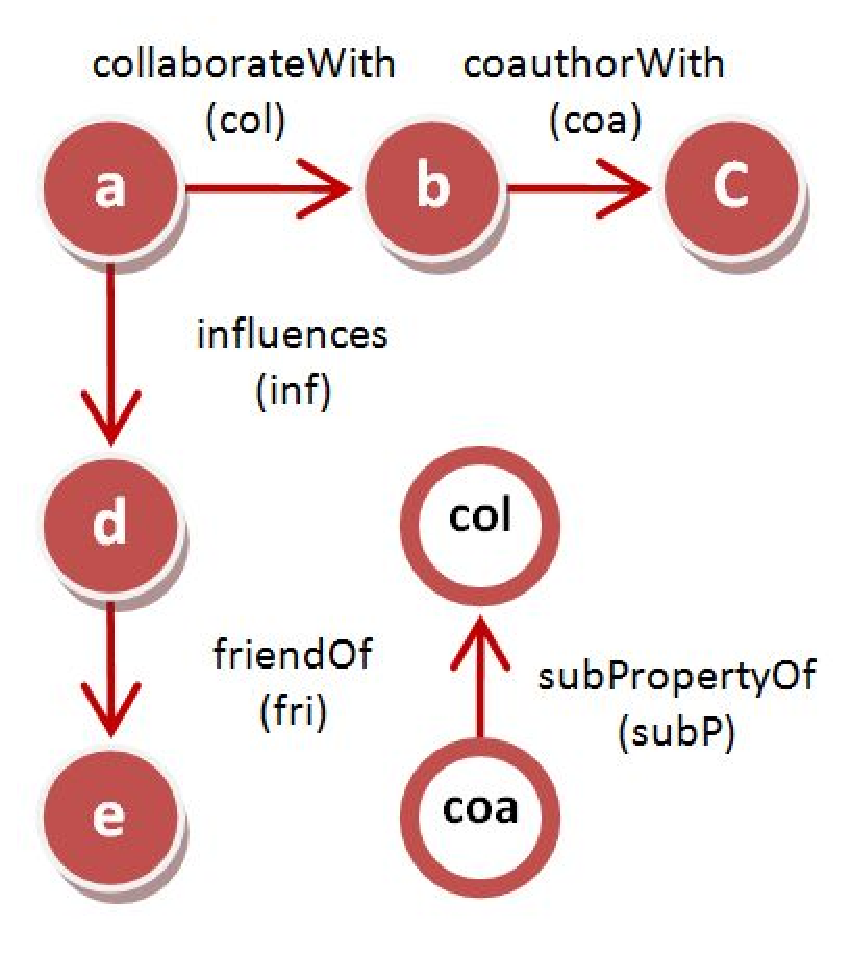
\includegraphics[width=.3\textwidth]{fig/reg_graph.eps} &
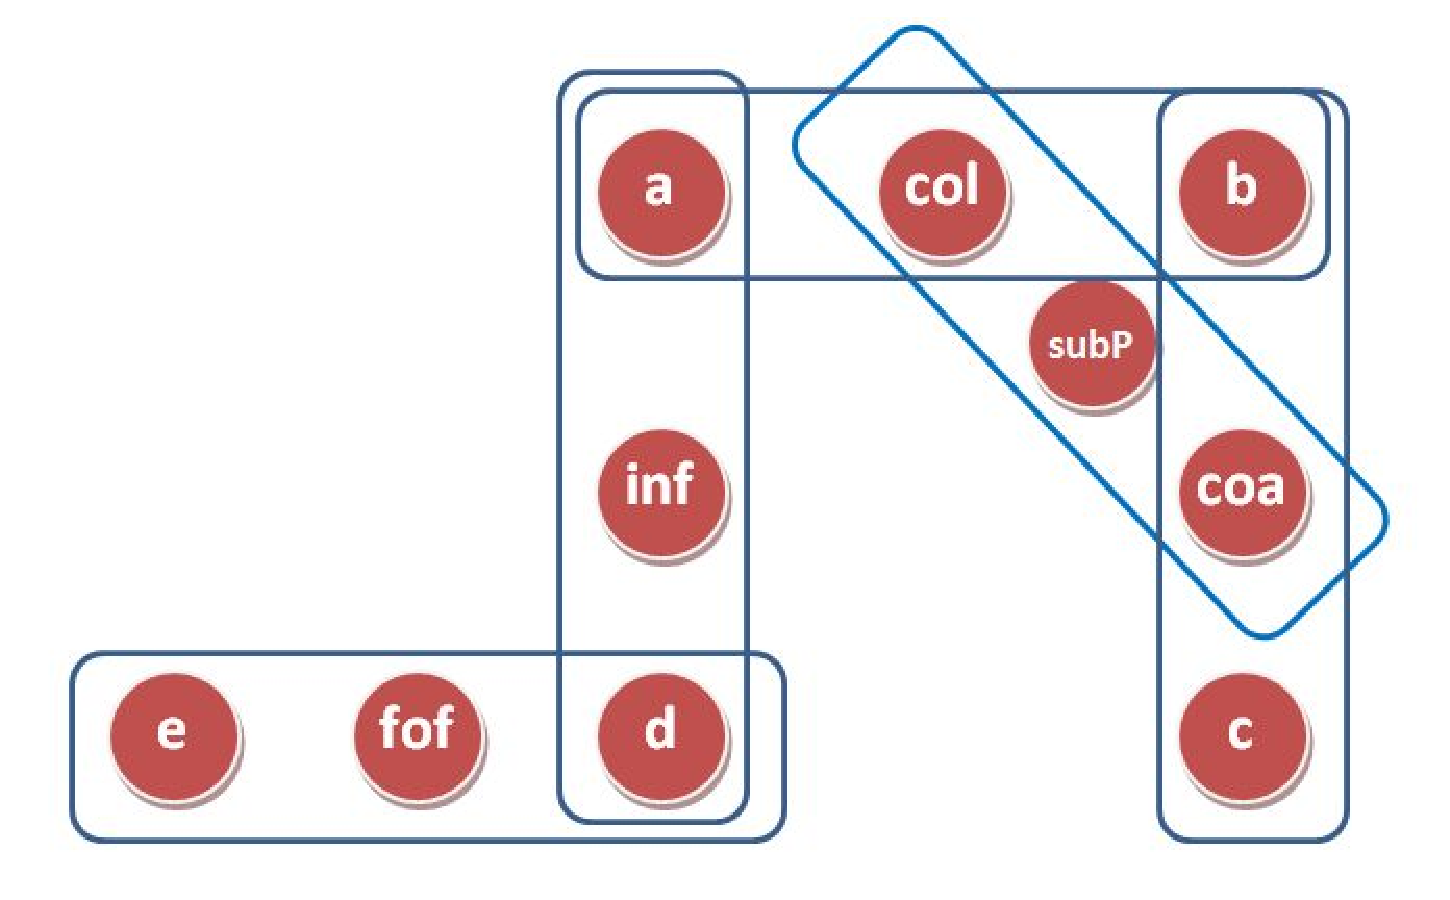
\includegraphics[width=.5\textwidth]{fig/hypergraph.eps}\\
(A) & (B)\\
\end{tabular}
\end{center}
\caption{\label{fig:graphcomp} An example of nodes connected by different links and some relationship between the links, represented by A) a simple graph, and B) a hypergraph.}
\end{figure}

In this example, two different levels of information are expressed. At the data level, the following statements describe the relationship between nodes representing people: $\langle a~ col~ b\rangle$, $\langle b~ coa~ c\rangle$, $\langle a~ inf~ d\rangle$ and $\langle d~ fri~ e\rangle$. At the schema level, another statement asserting that $coa$ is a sub-property of $col$: $\langle coa~ subP~ col\rangle$. In this case, $col$ and $coa$ become both nodes and edges in the directed labeled graph, causing the inconsistency (as depicted in Fig.~\ref{fig:graphcomp}(A). One way to overcome this is to model RDF as a hypergraph.

A hypergraph~\cite{Hypergraph} is a generalization of a traditional graph where edges, called hyperedges, can connect more than two vertices. If each edge in a hypergraph covers the same number of nodes, it's called $r$-uniform hypergraph, $r$ being the number of nodes on each edge. Any RDF Graph can be represented by a simple ordered 3-uniform hypergraph, in which an RDF triple corresponds to a hypergraph edge, the nodes being the subject, predicate and object in this order. In this way, both meta-data and data level statements can be integrated in a consistent model. In Fig.~\ref{fig:graphcomp}(b), the information in the above example is represented using a hypergraph.

%bipartite graph-on the one side are hypergraph edges (representing statements, depicted as blank circle nodes); on the other side are hypergraph nodes (representing subject, property, and object; subjects and objects are depicted as solid circles and properties are rectangles). The bipartite edges, labeled as S, P, and O to represent the role, indicate the incidence relationship between hypergraph nodes and edges.

\begin{comment}

\begin{figure}[tbh]
\begin{center}
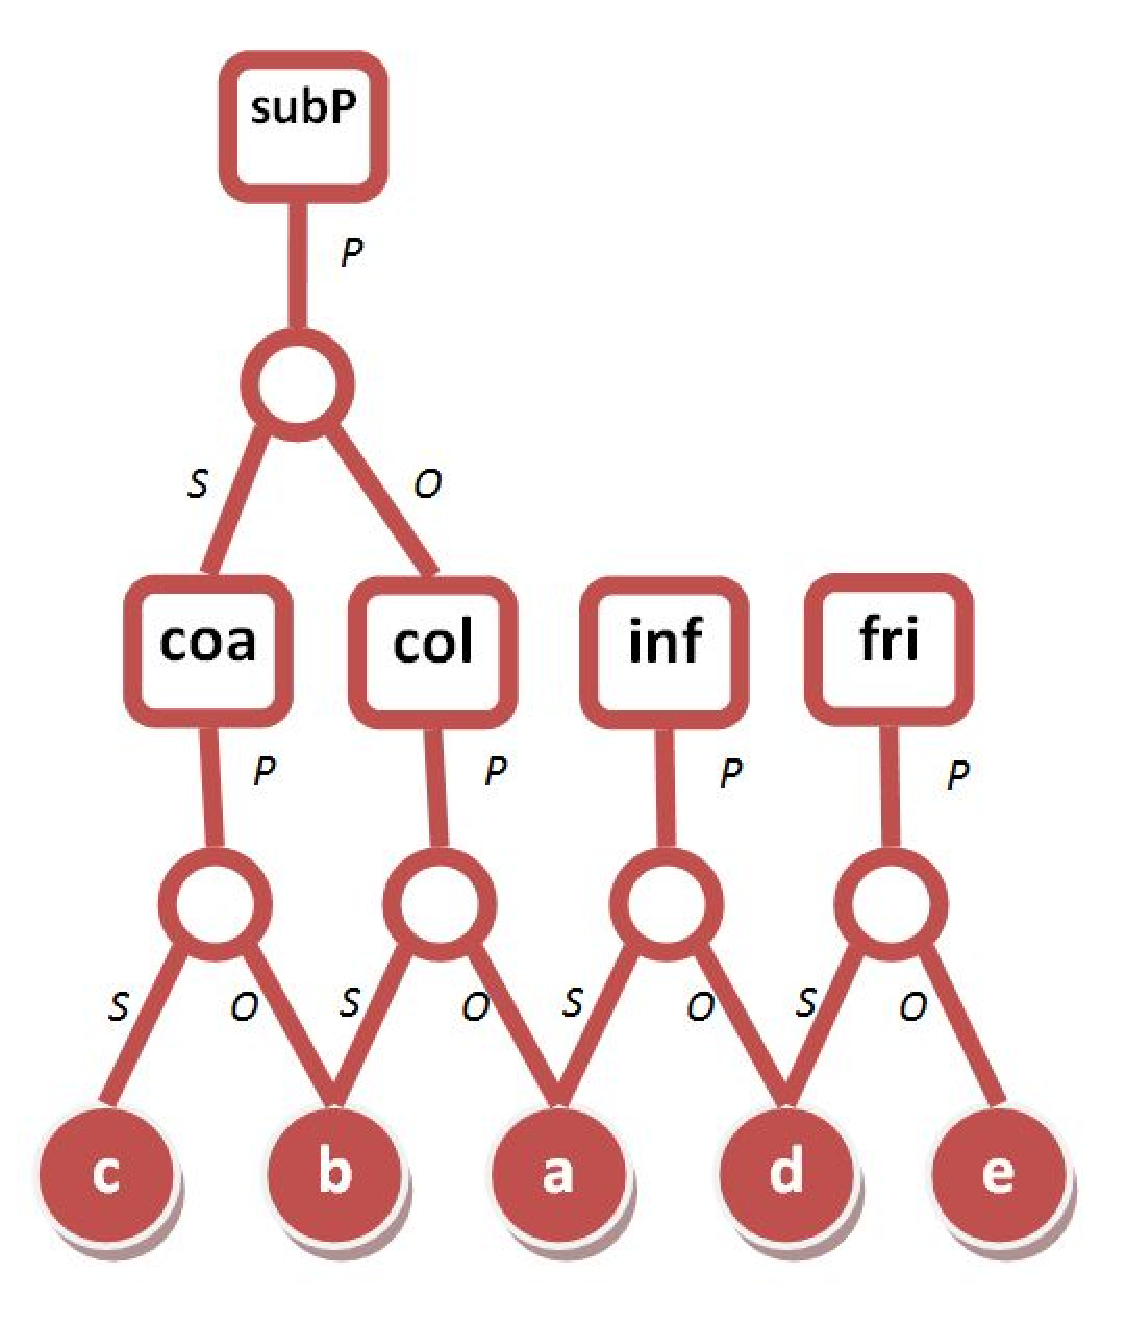
\includegraphics[width=.4\textwidth]{fig/BG.eps}
\end{center}
\caption{\label{fig:BG} .}
\end{figure}

\end{comment}

Formally, a hypergraph $G = (V,E)$, is a pair in which $V$ is the vertex set and $E$ is the hyperedge set where each $e \in E$ is a subset of $V$. A weighted hypergraph is a hypergraph that has a positive number $w(e)$ associated with each hyperedge $e$; called the weight of hyperedge $e$: Denote a weighted hypergraph by $G = (V,E,w)$. The degree of a vertex $v \in V$, $d(v)$, is defined as $d(v) = \sum_{v\in V, e\in E}{w(e)}$. The degree of a hyperedge $e$, denoted as $\delta(e)$, is the number of vertices in $e$, i.e. $\delta(e)=|e|$. A hyperedge $e$ is said to be incident with a vertex $v$ when $v \in e$. The hypergraph incidence matrix $\mathbf{H} \in \mathbb{R}^{|V| \times |E|}$ is defined as
\begin{equation}
\notag h(v,e)=\left\{\begin{array}{cl}
	   1, & v \in e \\
	   0, & otherwise
	   \end{array}\right.
\end{equation}
Throughout the rest of the dissertation, the diagonal matrix forms for $\delta(e)$, $w(e)$, $d(v)$ are denoted as $\mathbf{D}_e$, $\mathbf{W} \in \mathbb{R}^{|E|}$, and $\mathbf{D}_v \in \mathbb{Z}^{|V|}$, respectively.

\section{Graphs in Data Mining}
\subsection{Graph Representation of Relational Structure}
An object set endowed with pairwise relationships can be naturally illustrated as a graph in which vertices represent objects, and any two vertices that have some kind of relationship are joined together by an edge. In the case of frequent itemset mining, a set of objects with the co-occurrence relationship can be represented as directed or undirected graphs. For illustrating this point of view, let us consider a relational table depicted in Figure~\ref{fig:hg_and_rg}(a). One can construct an undirected graph where the set of vertices is the set of relational attributes (column items) and an edge joins two vertices if the they co-occur in a tuple (as illustrated in Figure~\ref{fig:hg_and_rg}(b)). This graph is called \emph{Gaifman graph}~\cite{Hodkinson02finiteconformal} of a relational structure. The undirected graph can be further enriched by assigning to each edge a weight equal to the support of the 2-itemset consisting of vertices incident to the edge. Cliques (complete subgraphs) in the Gaifman graph, or \emph{Gaifman cliques} for short, are of particular interest because every tuple (ground atom) in data corresponds to a Gaifman clique. However, ambiguity arises as not all Gaifman cliques have matching tuple in the data. There exists cases where cliques are incidental in the sense that several relational ground atoms play together to induce a clique configuration in the Gaifman graph, but no ground atom covers the entire clique (e.g., the clique of $\{A,B,C,D\}$ in Figure~\ref{fig:hg_and_rg}(b) does not correspond to any tuple in the relational table).

\begin{figure*}[tbh]
\begin{center}
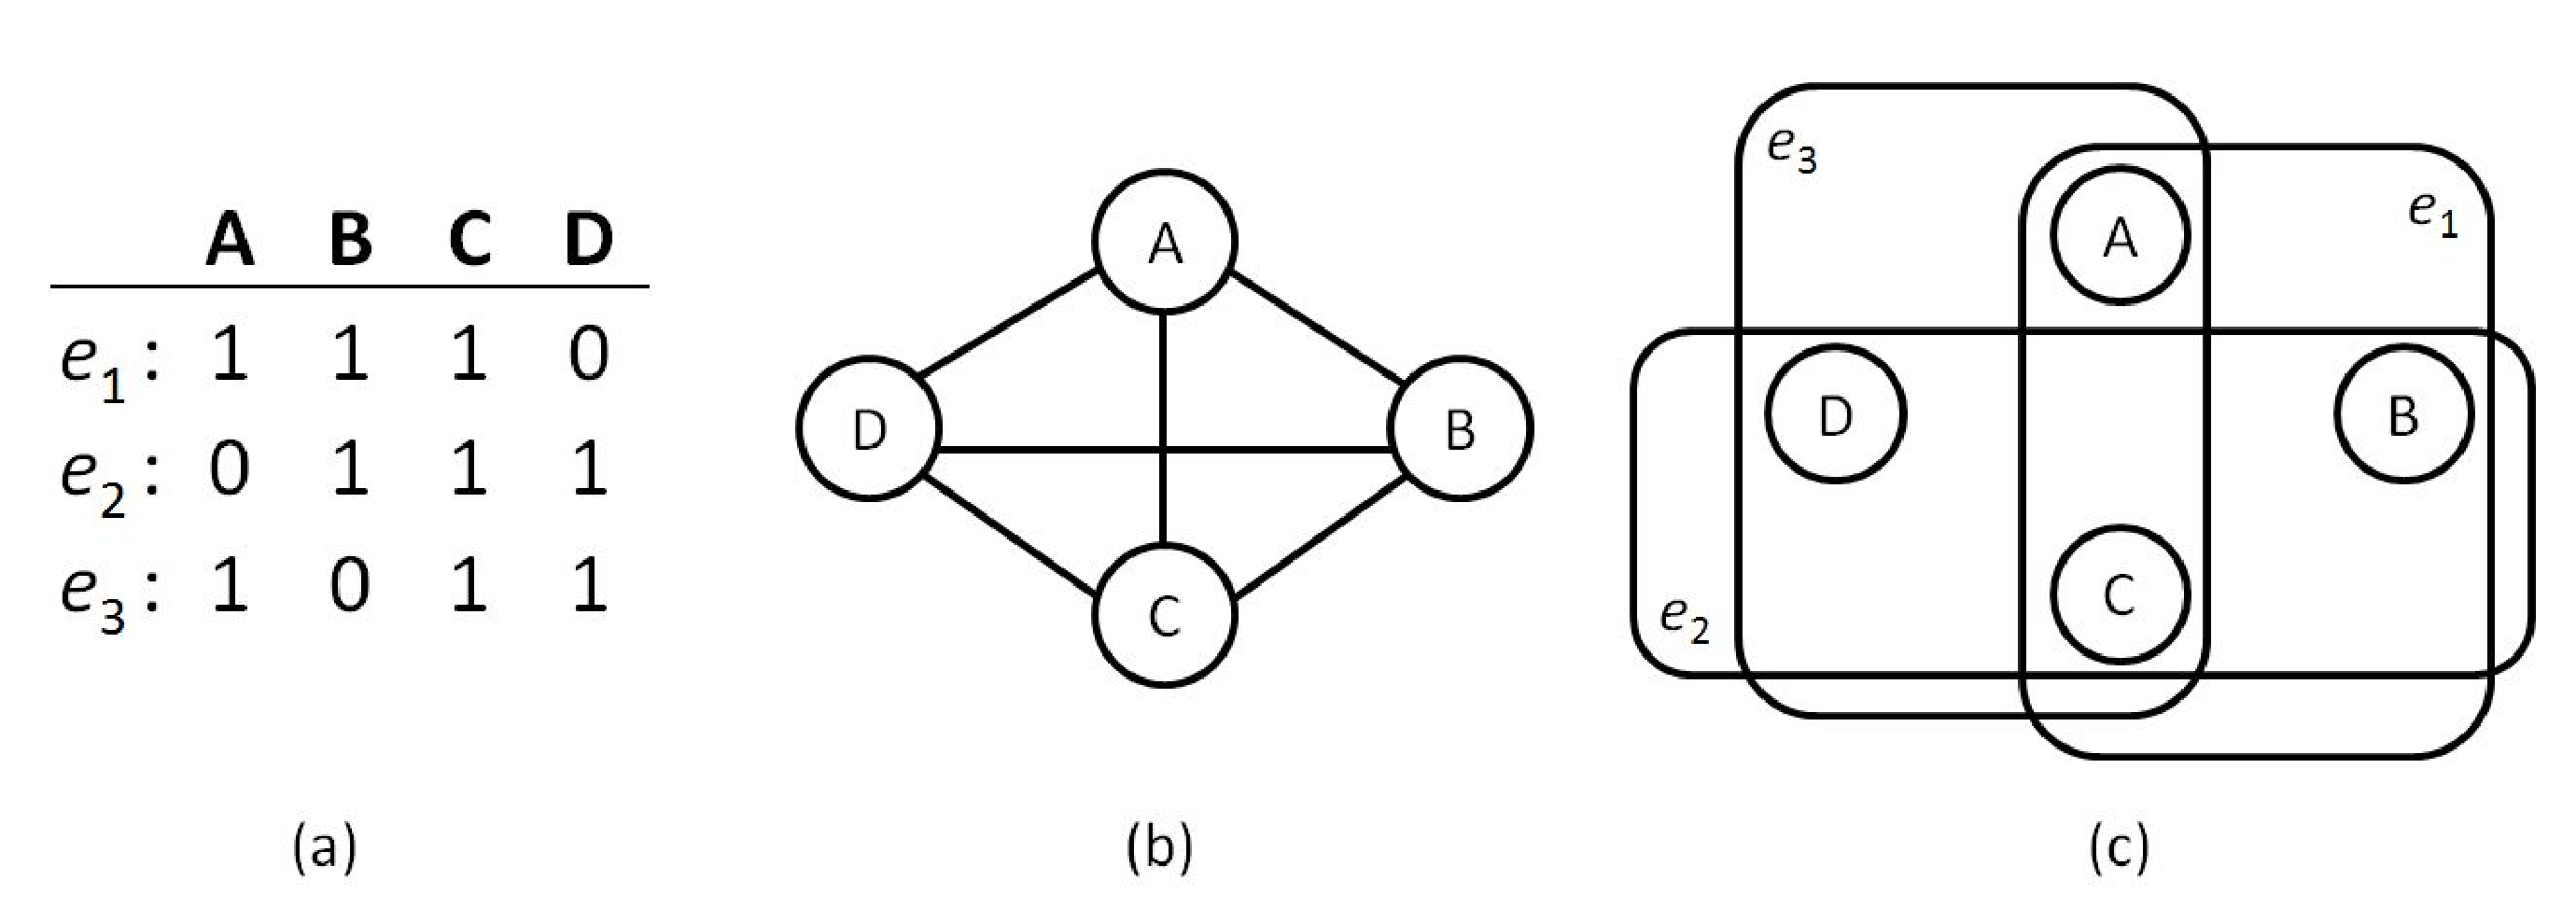
\includegraphics[width=.8\textwidth]{fig/hg_and_rg1.eps}
\end{center}
\caption{\label{fig:hg_and_rg} (a) an example transaction table; (b) the Gaifman graph representation of the table; (c) The hypergraph representation of the table}
\end{figure*}

A natural way to remedy the ambiguity is to represent the relational data as a \emph{hypergraph}~\cite{Hypergraph}. A hypergraph is a generalization of traditional graph. An edge in the hypergraph, called hyperedge, can connect more than two vertices. In other words, every hyperedge is an arbitrary nonempty subset of vertices. It is obvious that a simple graph is a special kind of hypergraph with each hyperedge containing only two vertices. In this paper, we propose to employ hypergraphs to model relational structure for finding semantically associated itemsets. Specifically, we propose to construct a hyperedge for each tuple. The relational attributes constitute the universe of vertices in the hypergraph. In this representation, each hyperedge has an exact one-to-one correspondent tuple (see Figure~\ref{fig:hg_and_rg}(c), for example).

\subsection{Similarity Measure}
%Sheth et al.~\cite{Sheth05semanticassociation} proposed a formalism for semantic association between entities in an RDF graph. Specifically, the semantic association is defined based on semantic connectivity which indicates if there exists a sequence of interconnected links between two given entities. In our study of semantically associated itemsets in transaction data, the link between entities is essentially the `co-occurrence' relationship. The semantic association according to Sheth et al's definition between transaction items $i_0$ and $i_n$ can be established by identifying a link of the form $i_0, P_c, i_1, P_c, \ldots, i_{n-1}, P_c, i_{n}$, in which $P_c$ denotes the co-occurrence property. The random walk model on hypergraph described in Section~\ref{sec:rw_hyper} formalizes this point of view. Our method for measuring the strength of semantic association is hence based on constructing a hypergraph representation and studying its property with both graph theoretical and spectral analysis techniques.

%Connectivity query between two nodes are essential in numerous mining tasks. Sheth et al.~\cite{Sheth05semanticassociation} defined semantic connectivity in RDF graph as follows. Two entities $e_1$ and $e_n$ are semantically connected if there exists a sequence $e_1, P_1, e_2, P_2, e_3, \ldots, e_{n-1}, P_{n-1}, e_n$ in an RDF graph where $e_i$ are entities and $P_j$ are properties. A sequence of alternating entities and properties represents a semantic path. Fig.~\ref{fig:graphcomp}(B) shows the connectivity between nodes c, a, and e. Paths connecting these nodes are colored in blue.

Given graph-based representation of information sources, meaningful similarity measure $s$ between nodes in the graph is critical in numerous data mining tasks. Take the simple network in Fig.~\ref{fig:graphcomp}(B) for example, suppose given a task of friend recommendation based on the information in this graph, the interesting question is whether $c$ or $e$ is a better choice of recommendation to $a$. To answer this question, it is natural to compare the similarity measures $s(a, c)$ and $s(a, e)$. In a rough sense, on can identify in the hypergraph representation that there are two paths between $a$ and $c$ (the formal definition for paths in hypergraphs will be given in Section~\ref{sec:rw_hyper}), while only one between $a$ and $e$. It's intuitive to conclude that $a$ and $c$ are more similar, or closer, than $a$ and $e$. This gives us a hint that meaningful similarity measures on the graph should satisfy the following intuitions:
\begin{enumerate}
\item The more paths connecting two nodes, the closer they are.
\item The shorter the paths, the closer they are.
\end{enumerate}
In other words, the more ``short" connections between two given nodes, the more similar those nodes are. To this end, we propose to employ the following quantities as the candidate similarity measure since both of them have the desired property. They are, namely, the \emph{commute time distance} based similarity measure from the random walk model on hypergraph, and the inner product similarity based on the \emph{pseudoinverse of the hypergraph Laplacian}. They are all based on the random walk model on hypergraph. In the following, we briefly introduce the theory of random walk.

\subsubsection{Random Walk}
\textbf{Random Walk on Simple Graph}
Given a graph and a starting point we select a neighbor of it at random and move to this neighbor then we select a neighbor of this point at random and move to it etc. The random sequence of points selected this way is a random walk on the graph. In other words, a random walker can jump from vertex to vertex and each vertex therefore represents a state of the Markov chain. The average first-passage time $m(k|i)$~\cite{randomwalks} is the average number of steps needed by a random walker for reaching state $k$ for the first time, when starting from state $i$. The symmetrized quantity $n(i,j)=m(j|i)+m(i|j)$ called the average commute time~\cite{randomwalks}, provides a distance measure between any pair of states. The fact that this quantity is indeed a distance on a graph was proved independently by Klein and Randic~\cite{Klein} and Gobel and Jagers~\cite{Gobel}.

%The average commute time has the nice property of decreasing when the number of paths connecting two vertices increases and when the ``length" of any path decreases, that is, when communication is facilitated. In short, the more short paths connect two given vertices, the more similar those vertices are. The ``shortest path" or ``geodesic" distance does not have the nice property of decreasing when connections between nodes are added: It does not capture the fact that strongly connected nodes are at a smaller distance than weakly connected ones.

The Laplacian matrix $\mathbf{L}$ of a graph is widely used for finding many properties of the graphs in spectral graph theory. Given node degree matrix $\mathbf{D}$ and graph adjacency matrix $\mathbf{A}$, the Laplacian matrix of the graph is defined as $\mathbf{L}=\mathbf{D}-\mathbf{A}$. The normalized Laplacian is given by $\mathbf{L}_N=\mathbf{I}-\mathbf{D}^{-1/2}\mathbf{A}\mathbf{D}^{-1/2}$, where $\mathbf{I}$ is the identity matrix. The average commute time $n(i,j)$ can be computed in closed form from the Moore-Penrose pseudoinverse of $\mathbf{L}$~\cite{pseudo}, denoted by $\mathbf{L}^+$.

Various quantities derived from random walk on graph has been used in a number of applications. Fouss et al.~\cite{Fouss06random-walkcomputation} compared twelve scoring algorithms based on graph representation of the database to perform collaborative movie recommendation. Pan et al.~\cite{Pan} developed a similarity measure based on random walk steady state probability to discover correlation between multimedia objects containing data of various modalities. Yen et al.~\cite{Yen05clusteringusing} introduced a new k-means clustering algorithm utilizing the random walk average commute time distance. Zhou et al.~\cite{Zhou:2009:GCB:1687627.1687709} presented a unified framework based on neighborhood random walk to integrate structural and attribute similarities for graph clustering.



\begin{comment}

The field of graph mining has seen a rapid explosion in recent years because of new applications in computational biology, software bug localization, and social and communication networking. This book is designed for studying various applications in the context of managing and mining graphs. Graph mining has been studied by the theoretical community extensively in the context of numerous problems such as graph partitioning, node clustering, matching, and connectivity analysis. However the traditional work in the theoretical community
cannot be directly used in practical applications because of the following reasons:

The definitions of problems such as graph partitioning, matching and dimensionality reduction are too ``clean" to be used with real applications. In real applications, the problem may have different variations such as a disk-resident case, a multi-graph case, or other constraints associated with the graphs. In many cases, problems such as frequent sub-graph mining and dense graph mining may have a variety of different flavors for different scenarios.

The size of the applications in real scenarios are often very large. In such cases, the graphs may not be stored in main memory, but may be available only on disk. A classic example of this is the case of web and social network graphs, which may contain millions of nodes. As a result, it is often necessary to design specialized algorithms which are sensitive to disk access efficiency constraints. In some cases, the entire graph may not be available at one time, but may be available in the form of a continuous stream. This is the case in many applications such as social and telecommunication networks in which edges are received continuously.

It is assumed that the underlying graphs are massive and cannot be held in main memory. This change in assumption has a critical
impact on the algorithms which are required to process such graphs. The problems studied in the book include algorithms for frequent pattern mining, graph matching, indexing, classification, clustering, and dense graph mining. In many cases, the problem of graph management and mining has been studied from the perspective of structured and XML data. Where possible, we have clarified the
connections with the methods and algorithms designed by the XML data management community. We also provide a detailed discussion of the application of graph mining algorithms in a number of recent applications such as graph privacy, web and social networks.

Many of the graph algorithms are sensitive to the application scenario in which they are encountered. Therefore, we will study the usage of many of these techniques in real scenarios such as the web, social networks, and biological data. This provides a better understanding of how the algorithms in the book apply to different scenarios. Thus, the book provides a comprehensive summary both from an algorithmic and applied perspective.
\end{comment} 

%%%%%%%%%%%%%%%%%%%%%%%%%%%%%%%%%%%%%%%%%%%%%%%%%%%%%%%%%%%%%%%%%%%

\chapter{GRAPH REPRESENTATION}
\label{chap:representation}
%\section{Representing Domain Knowledge and Data using Graphs}
The interface between domain knowledge and data is achieved by employing the RDF model and by the fact that RDF allows a combined specification of both schema and data structured under this schema.

RDF's abstract triple syntax has a graph nature. Graphs are mathematical objects that enjoy wide-spread usage for many tasks, which include the visualization and analysis of data for humans, mathematical reasoning, and the implementation as a data structure for developing data mining algorithms. Besides the common graph-theoretic model of RDF as labeled, directed multi-graphs, Hayes has established that RDF can be also represented as hypergraphs (bipartite graphs)~\cite{GraphModelRDF}. This result constitutes an important aspect of the theoretical basis of this proposal and is discussed in sections below. We propose to use the graph-based representation for RDF as a combined information source of both domain knowledge and data for different mining tasks, including association rule mining, classification, clustering and so forth.

\section{Graph Representation for Domain Knowledge}
Graph-based approaches for representing knowledge have long been used in philosophy, psychology, and linguistics. The computer counterpart to this means is the so-called \emph{semantic network} that represents knowledge in patterns of interconnected nodes and arcs which were first developed for artificial intelligence and machine translation.

The semantic network, and graph-based approaches for KR in general, are motivated by the desirable qualities of graph for both modeling and computation. From a modeling viewpoint, basic graphs are easily understandable by users, and it is always possible to split up a large graph into smaller ones while keeping its semantics. From the computational viewpoint, graph is one of the most studied objects in mathematics. Considering graphs instead of logical formulas provides another view of knowledge constructs (\eg, some notions like path, cycle, or connected components are natural on graphs) and provides insights to algorithmic ideas~\cite{CheinMugnier08}. In light of these motivations, what is common to all semantic networks is a declarative graphic representation that can be used either to represent knowledge or to support automated systems for reasoning about knowledge.

Among all variants of semantic networks, we emphasize the most on the usage of definitional networks to incorporate domain knowledge in data mining. The kind of knowledge that are best captured by this kind of network is subsumption hierarchy, on which a distance (similarity) measure can be reasonably defined. Such measure is essential in many data mining tasks. It is possible to extend, in a straightforward manner, data mining algorithms that depend on analyzing distances between entities in factual knowledge to work with distances between those in ontological knowledge.

In addition, one of the most prominent KR formalism families among current systems of definitional networks, description logics (DLs), formerly called terminological logics or concept languages, have been a successful attempt to combine well-defined logical semantics with efficient reasoning~\cite{Sowa91principlesof}. They are derived from an approach proposed by Woods~\cite{woods75link} and implemented by Brachman~\cite{Brachman91livingwith} in a system called Knowledge Language One (KL-ONE). Recent description logics are DAML+OIL~\cite{Horrocks02daml+oil} and its successor OWL, which are intended for representing knowledge in the semantic web~\cite{Berners-Lee01}--a giant semantic network that spans the entire Internet.

OWL ontologies can be used along with information written in RDF, and OWL ontologies themselves are primarily exchanged as RDF documents. RDF's abstract triple syntax has a graph nature. The RDF graph is defined as follows according to the W3C specification for RDF semantics~\cite{Hayes_rdf2004}:

\begin{mydef}[\textbf{RDF Graph}]
An RDF graph is defined as a set of RDF triples. A subgraph of an RDF graph is a subset of the triples in the graph. A triple is identified with the singleton set containing it, so that each triple in a graph is considered to be a subgraph. A proper subgraph is a proper subset of the triples in the graph. A ground RDF graph is one with no blank nodes.
\end{mydef}

RDF triples can be visualized as a \emph{directed labeled graph} as follows:
\begin{center}\ovalbox{subject} $\stackbin[]{predicate}{\xrightarrow{\hspace*{2cm}}}$ \ovalbox{object}\;,\end{center}
where subjects and objects are represented as nodes, and predicates as edges. The directed labeled graph model for RDF is straightforward and convenient in most cases. But inconsistency arises when using triples to make assertions on predicates. The directed labeled graph model of RDF makes the artificial distinction between resources and properties, which may cause inconsistency in the graph representation. The following example illustrates this point of view.

\begin{figure}[tbh]
\begin{center}
\begin{tabular}{ccc}
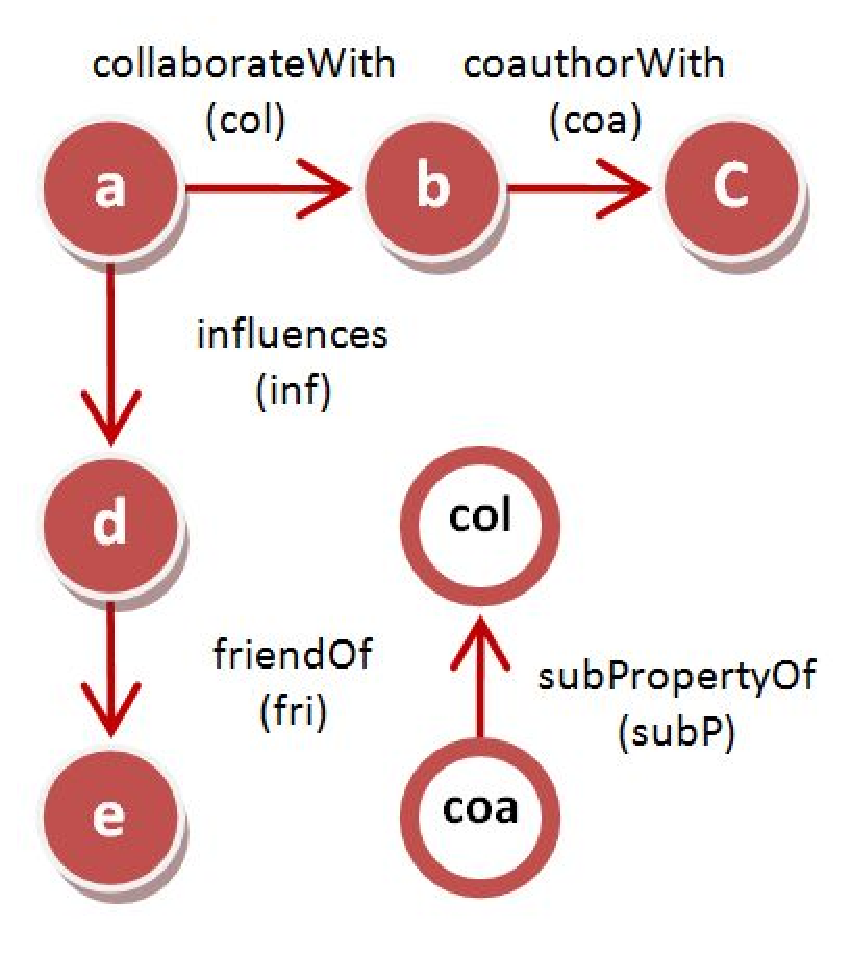
\includegraphics[width=.25\textwidth]{fig/reg_graph.eps} & &
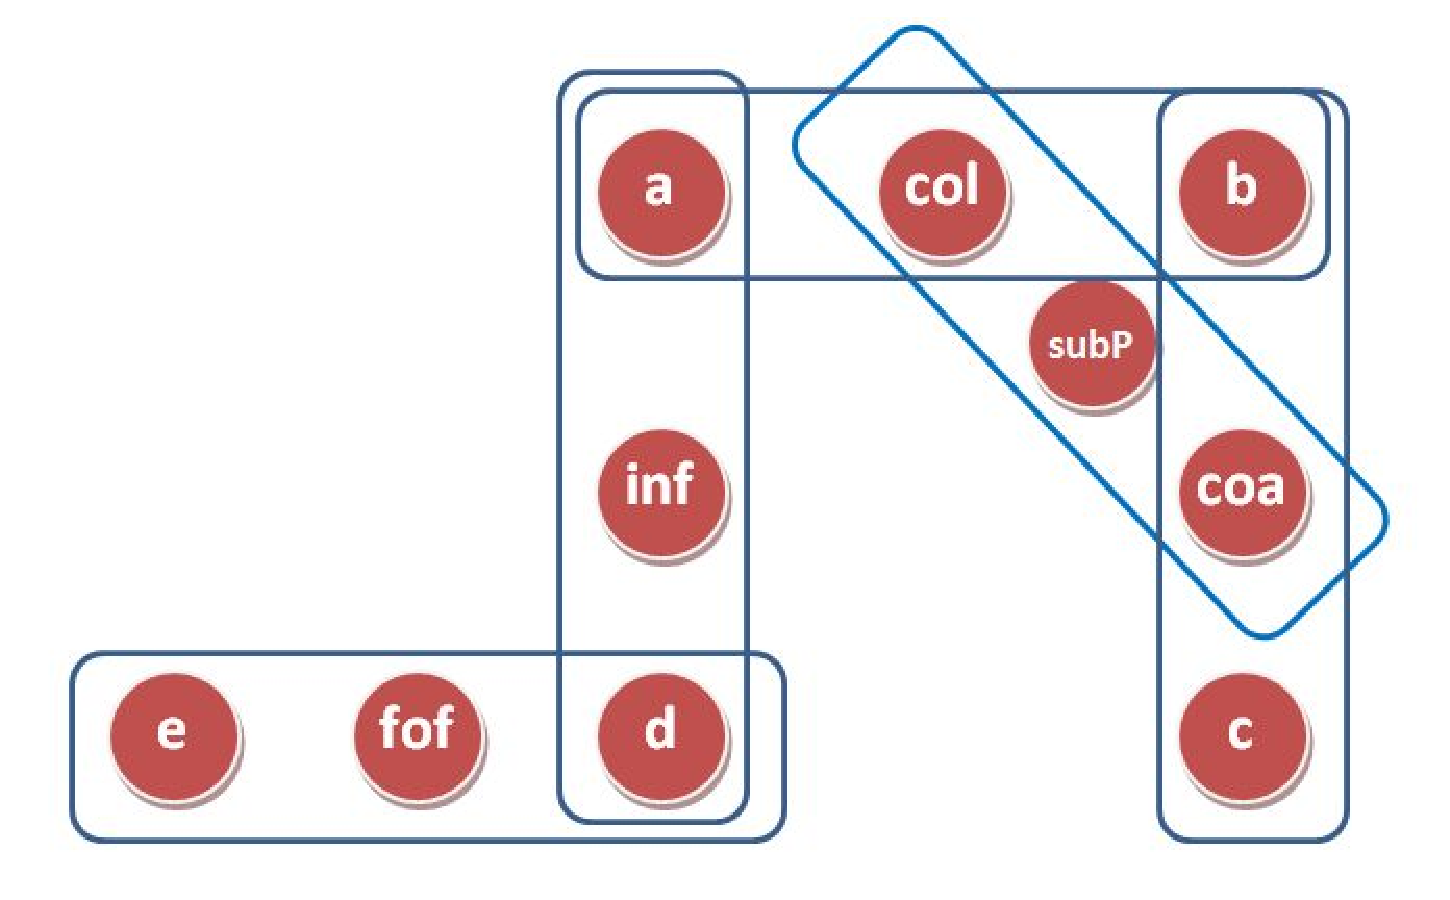
\includegraphics[width=.43\textwidth]{fig/hypergraph.eps}\\
(A) & & (B)\\
\end{tabular}
\end{center}
\caption[A comparison between a simple graph and a hypergraph]{\label{fig:graphcomp} An example of nodes connected by different links and some relationship between the links, represented by A) a simple graph, and B) a hypergraph.}
\end{figure}

\begin{myexp}[\textbf{Inconsistent representation of RDF directed labeled model}]
\label{graphcomp}
In this example, a set of RDF statements is asserted to describe the relationship among a group of people. The information expressed include two different levels, i.e., the meta (ontological) data and factual data. The factual data level consists of following statements: $\langle a~ collaborate~ b\rangle$, $\langle b~ coauthor~ c\rangle$, $\langle a~ influence~ d\rangle$ and $\langle d~ friendOf~ e\rangle$. The meta-data level contains one single statement asserting that $coauthor$ is a sub-property of $collaboration$: $\langle coauthor~ subProperty~ collaboration\rangle$. In this case, the representation of $collaboration$ and $coauthor$ is inconsistent. They are represented as nodes at the factual data level and edges at the meta-data level (see Figure~\ref{fig:graphcomp}(A)).
\end{myexp}

To overcome this, Hayes et al.~\cite{GraphModelRDF} proposed to model RDF as a \emph{hypergraph}. A hypergraph~\cite{Hypergraph} is a generalization of a traditional graph where edges, called hyperedges, can connect more than two vertices. If each edge in a hypergraph covers the same number of nodes, it's called $r$-uniform hypergraph, $r$ being the number of nodes on each edge. Any RDF Graph can be represented by a simple ordered 3-uniform hypergraph, in which an RDF triple corresponds to a hypergraph edge, the nodes being the subject, predicate and object in this order. In this way, both meta-data and data level statements can be integrated in a consistent model.

In Fig.~\ref{fig:graphcomp}(B), the information in the Example~\ref{graphcomp} is represented by a hypergraph and the inconsistency in the directed labeled graph representation is eliminated.

\begin{mydef}[\textbf{Hypergraph}]
Formally, a hypergraph $G = (V,E)$, is a pair in which $V$ is the vertex set and $E$ is the hyperedge set where each $e \in E$ is a subset of $V$. A weighted hypergraph is a hypergraph that has a positive number $w(e)$ associated with each hyperedge $e$; called the weight of hyperedge $e$: Denote a weighted hypergraph by $G = (V,E,w)$. The degree of a vertex $v \in V$, $d(v)$, is defined as $d(v) = \sum_{v\in V, e\in E}{w(e)}$. The degree of a hyperedge $e$, denoted as $\delta(e)$, is the number of vertices in $e$, i.e. $\delta(e)=|e|$. A hyperedge $e$ is said to be incident with a vertex $v$ when $v \in e$. The hypergraph incidence matrix $\mathbf{H} \in \mathbb{R}^{|V| \times |E|}$ is defined as
\begin{equation}
\notag h(v,e)=\left\{\begin{array}{cl}
	   1, & v \in e \\
	   0, & otherwise
	   \end{array}\right.
\end{equation}
Throughout the rest of the paper, the diagonal matrix forms for $\delta(e)$, $w(e)$, $d(v)$ are denoted as $\mathbf{D}_e$, $\mathbf{W} \in \mathbb{R}^{|E|}$, and $\mathbf{D}_v \in \mathbb{Z}^{|V|}$, respectively.
\end{mydef}

A hypergraph $G = (V, E)$ can be transformed to a \emph{bipartite graph} $BG$ as follows:

\begin{mydef}[\textbf{Transformation from RDF hypergraph to RDF bipartite graph}]
Let the sets $V$ and $E$ are the partitions of $BG$. The node pair $(v_1, e_1)$ is connected with an edge if and only if vertex $v_1$ is contained in edge $e_1$ in $H$. Conversely, any bipartite graph with fixed parts and no unconnected nodes in the second part represents some hypergraph in the manner described above. This bipartite graph can be represented by incidence matrices. Such a matrix can be understood as the node adjacency matrix of a bipartite graph.
\end{mydef}
\begin{figure}[tbh]
\centering
\begin{minipage}[c]{0.58\textwidth}\centering
\[ \bordermatrix{ ~       &  \text{~a~}  &  \text{~b~}  &  \text{~c~}  &  \text{~d~}  &  \text{~e~}  &   \text{coa} &   \text{col} &   \text{inf} &   \text{fof} &   \text{subP}\cr
                  E_1~~   &   1   &   1   &       &       &       &       &   1   &       &       &       \cr
                  E_2~~   &       &   1   &   1   &       &       &   1   &       &       &       &       \cr
                  E_3~~   &   1   &       &       &   1   &       &       &       &   1   &       &       \cr
                  E_4~~   &       &       &       &   1   &   1   &       &       &       &   1   &       \cr
                  E_5~~   &       &       &       &       &       &   1   &   1   &       &       &    1}
\]
\end{minipage}
\hfill
\begin{minipage}[c]{0.38\textwidth}\centering
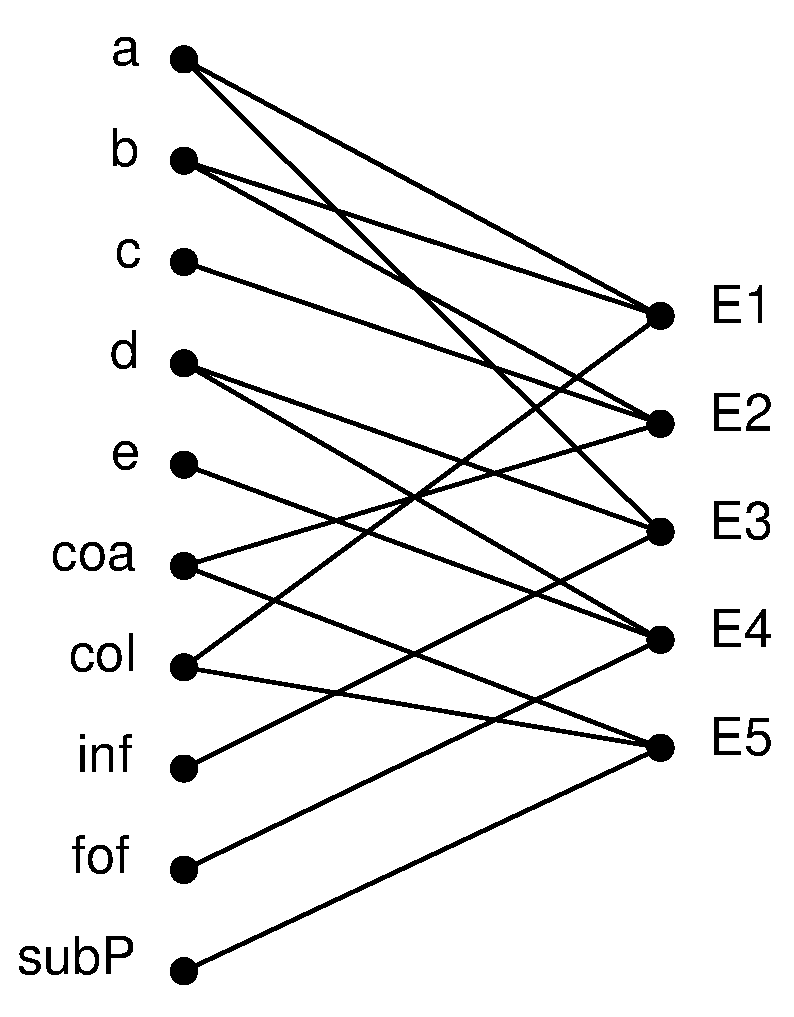
\includegraphics[width=.7\textwidth]{fig/BG-black.eps}
\end{minipage}
\caption[An example incidence matrix of a hypergraph]{\label{fig:incidence}Incidence matrix representing the hypergraph of figure~\ref{fig:graphcomp}(B) and the corresponding incidence graph.}
\end{figure}

RDF bipartite graphs have many desirable properties for developing intuitive mining algorithms. Thus, the we propose to use bipartite graphs to represent domain knowledge and data expressed in RDF.

\begin{myexp}[\textbf{Hypergraph incidence matrix and corresponding bipartite graph}]
\label{incidence}
Figure~\ref{fig:incidence} (A) shows the incidence matrix according to the hypergraph in Figure~\ref{fig:graphcomp} for Example~\ref{graphcomp}. Figure~\ref{fig:incidence} (B) shows the corresponding bipartite graph. Hypergraph incidence matrices represent membership of a node in an edge with a ``1" in the corresponding entry.
\end{myexp}

Example~\ref{incidence} illustrates the general method that can be applied to all hypergraphs to transform to their bipartite graph form. In the case of a hypergraph representing an RDF Graph, since nodes in a RDF statement are ordered (subject followed by predicate then object), this ordering must be preserved in the incidence matrix. A \emph{labeled bipartite graph} can be derived to further capture the ordering and roles of nodes.

\begin{mydef}[\textbf{RDF labeled bipartite graph}]
In the hypergraph incidence matrix, instead of using ``1/0'' according to the occurrence of a node in an hyperedge, we choose to label them by S, P or O to represent the role (subject, predicate, or object) of the node in that underlying RDF statement--edge. Hence, when deriving the bipartite graph of a hypergraph incidence matrix, an edge will be added for every S, P, O entry of the matrix, and this edge will be labeled with the corresponding character (S, P, or O). Thus, the only difference between the graph derived from the incidence matrix of any hypergraph and an RDF Graph hypergraph is the fact that each edge has one out of three labels~\cite{GraphModelRDF}.
\end{mydef}

In the rest of the proposal, when we use RDF bipartite graph, we mean RDF labeled bipartite graph for short.

\begin{myexp}[\textbf{RDF labeled bipartite graph}]
Figure~\ref{fig:graphcomp-bio} illustrates an example of RDF hypergraph represented as labeled bipartite graph. The left side shows a portion of an ontology in biomedical domain on zebrafish anatomy~\cite{ZFA} visualized as a directed labeled graph. Two different relationships are depicted in the figure, namely, ``subClassOf" and ``part\_of". The corresponding labeled bipartite graph representation is shown on the right side. Circle nodes are the \emph{statement nodes} representing the RDF statements. Each statement node is connected to three \emph{value nodes} representing the three components of a statement (subject, predicate, and object). Edge labels S, P, and O indicate the role of the value nodes in the statement.
\end{myexp}

\begin{figure}[tbh]
\centering
\begin{minipage}[c]{0.35\textwidth}\flushright
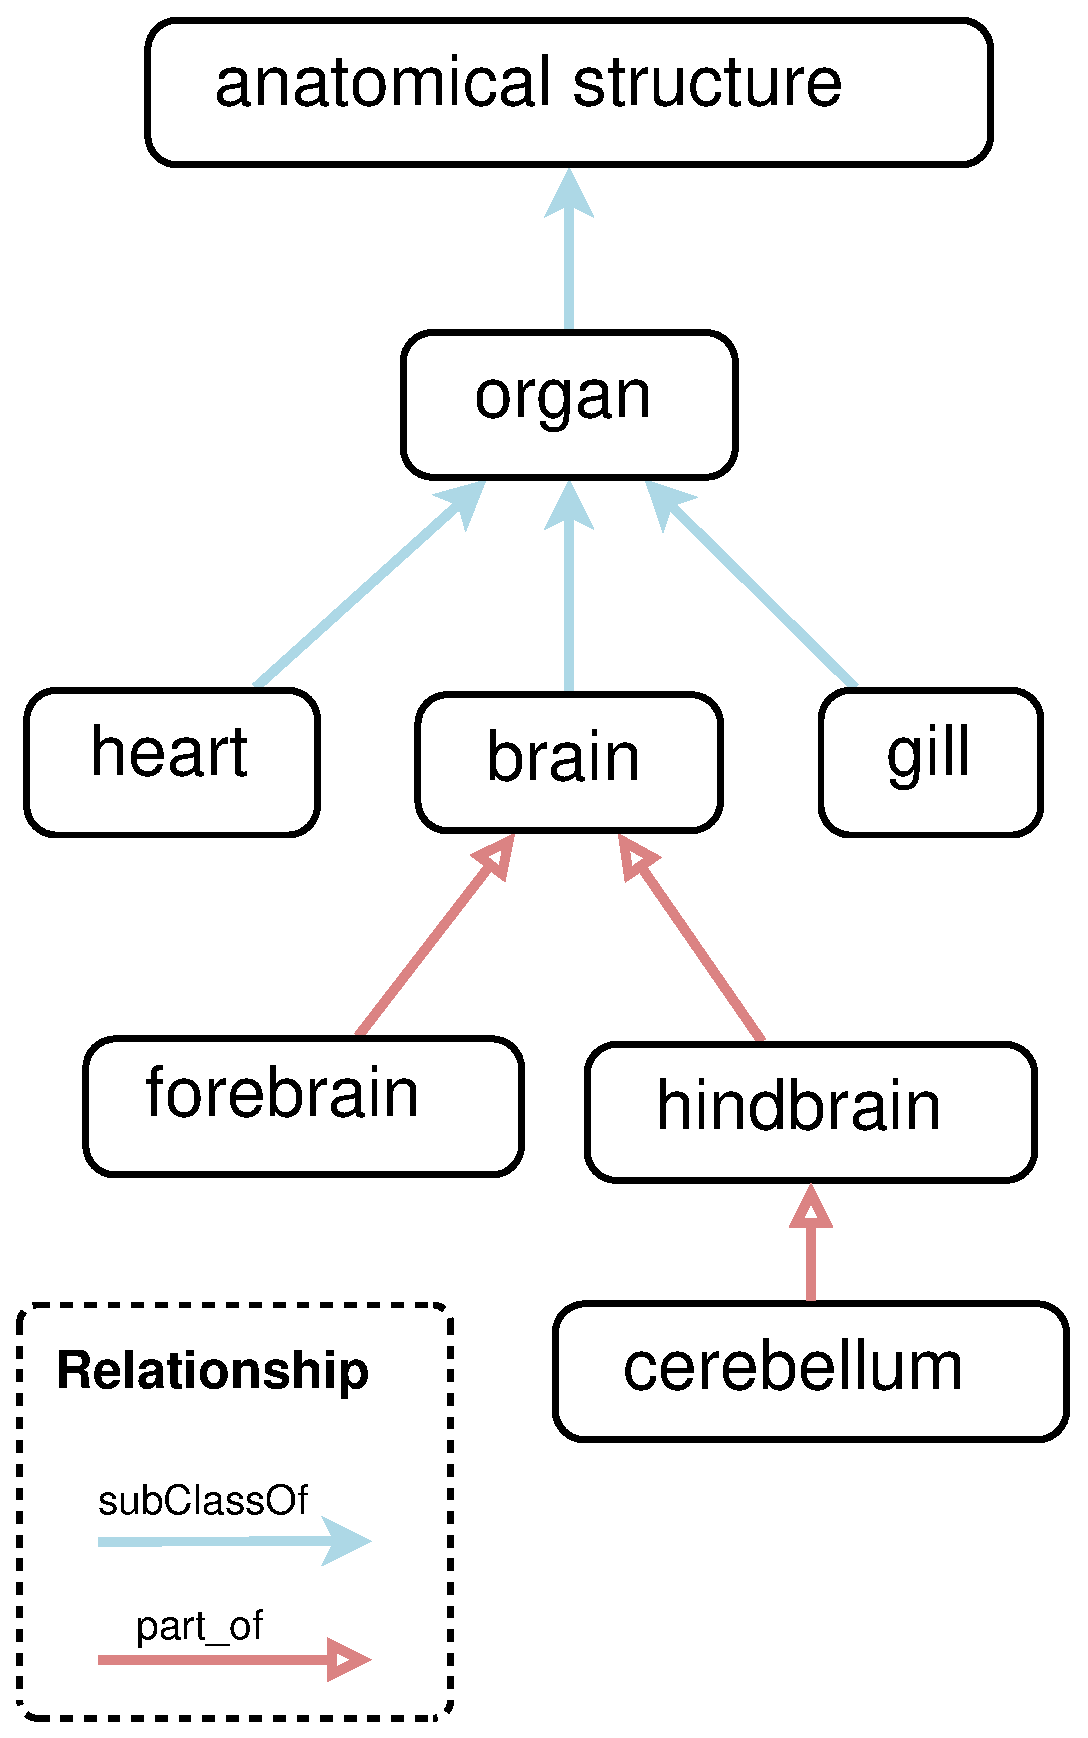
\includegraphics[width=.7\textwidth]{fig/DLG-bio.eps}
\end{minipage}\hfill
\begin{minipage}[c]{0.6\textwidth}\centering
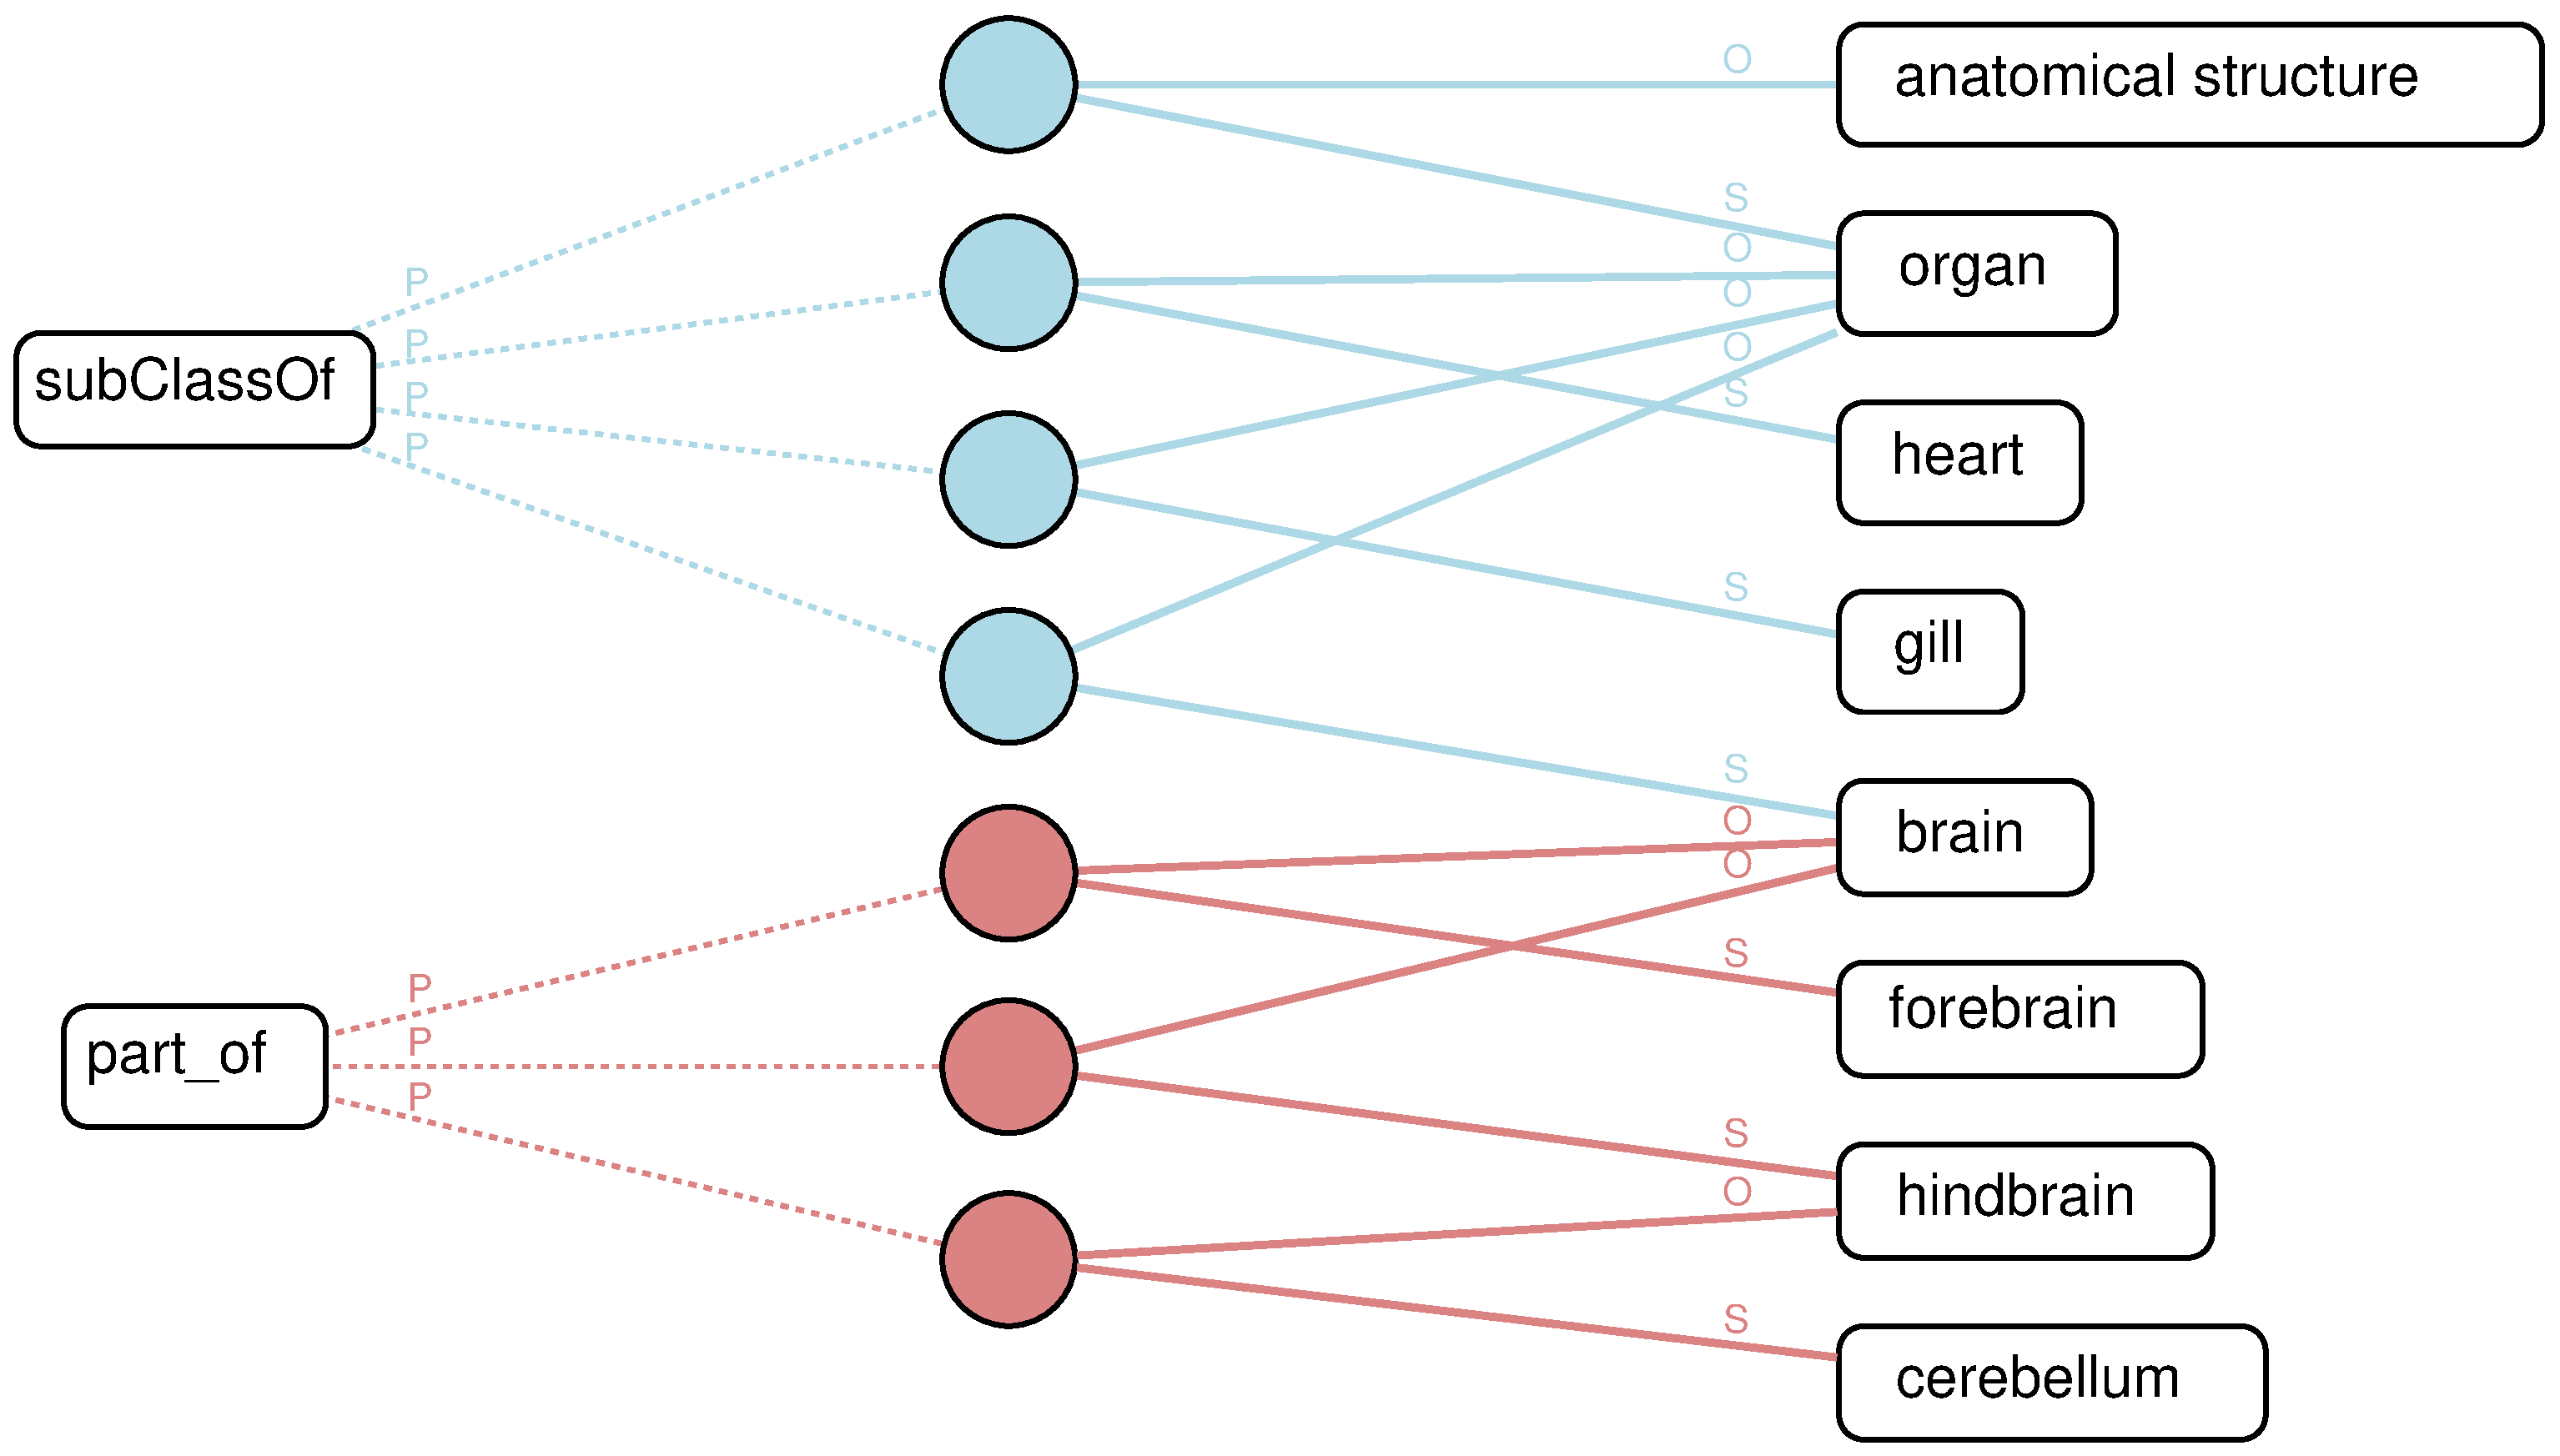
\includegraphics[width=\textwidth]{fig/BG-bio.eps}\\
\end{minipage}
\caption[A comparison between the directed labeled graph and the RDF bipartite graph]{\label{fig:graphcomp-bio} A portion of a zebrafish anatomy ontology represented as a directed labeled graph (A) and a RDF bipartite graph (B)}
\end{figure}

\section{Graph Representation for Relational Structure}
\label{sec:graph-rep-for-rdb}
Various graph representation for relational structure has been proposed in literature to tackle different data mining tasks. In the case of frequent itemset mining, a set of objects with the co-occurrence relationship can be represented as directed or undirected graphs (see the example in Figure~\ref{fig:hg_and_rg}).

Another way to represent relational structure is to first transform it to RDF, and by utilizing the graph nature of RDF, the relational structure can then be represented as graphs. Mapping from RDB to RDF has gained increasing attention and led to implementation of generic mapping tools as well as domain--specific applications.  The W3C launched the RDB2RDF incubator group to explore issues involved in mapping RDB to RDF. A work-in-progress survey paper has been published documenting approaches in this field~\cite{RDB2RDF}.

%We can classify the methods used to generate the mappings between RDB and RDF into two categories:
A straightforward method for mapping RDB to RDF is discussed by Berners Lee~\cite{TBL98} as defined in the following.

\begin{mydef}[\textbf{Context--independent mapping from RDB to RDF}]
Without linking to any explicit definition of domain semantics (such as those defined in domain ontologies), a RDB can be transformed to RDF following the steps below:
\begin{enumerate}
\label{auto-map}
\item A RDB row is a RDF subject node.
\item The column name of a RDB table is a predicate node.
\item A RDB table cell is an object node.
\end{enumerate}
\end{mydef}

Many systems leverage these mappings to automatically generate mappings between RDB and RDF. Even though these automatically generated mappings often do not capture complex domain semantics that are required by many applications, these mappings can serve as a useful starting point to create more customized, domain--specific mappings.

\begin{myexp}[\textbf{RDF bipartite graph for a nominal-valued RDB}]
Table~\ref{tbl:nominal-rel} (A) shows a relational table with nominal features (columns). The table has $m$ rows, each one annotated on the border with labels $r_1 \ldots r_m$, and $n$ columns named $f_1 \ldots f_n$. Applying the steps in Definition~\ref{auto-map} for mapping RDB to RDF mapping, the corresponding RDF statements are listed in Table~\ref{tbl:nominal-rel} (B). From these statements, a RDF bipartite graph is derived, shown in Figure~\ref{fig:BG-relational-nominal}, as the graph representation for the underlying relational table in Table~\ref{tbl:nominal-rel} (A).
\end{myexp}

\begin{table}[ht]
\begin{minipage}[c]{0.4\linewidth}\begin{flushright}
\begin{tabular}{ c | c | c | c |}
\cline{2-4}
	~   & $f_1$	    & $\cdots$  & $f_n$   \\
\cline{2-4}
$r_1:$	& $v_{11}$	& $\cdots$  & $v_{1n}$\\
\cline{2-4}
$\vdots$& $\vdots$  & $\ddots$  & $\vdots$\\
\cline{2-4}
$r_m:$	& $v_{m1}$	& $\cdots$  & $v_{mn}$\\
\cline{2-4}
\end{tabular}
\end{flushright}
\end{minipage}
\hfill
\begin{minipage}[c]{0.4\linewidth}
\begin{tabular}{c c c}
\emph{s}&   \emph{p}&  \emph{o}\\
\texttt{<$r_1$>}   &  \texttt{<$f_1$>}  &  \texttt{<$v_{11}$>}\\
\texttt{<$r_1$>}   &  \texttt{<$f_n$>}  &  \texttt{<$v_{1n}$>}\\
\texttt{<$r_m$>}   &  \texttt{<$f_1$>}  &  \texttt{<$v_{m1}$>}\\
\texttt{<$r_m$>}   &  \texttt{<$f_n$>}  &  \texttt{<$v_{mn}$>}\\
\end{tabular}
\end{minipage}
\begin{minipage}[c]{0.4\linewidth}\centering
\vspace{0.2cm}\hspace{2.8cm}(A)
\end{minipage}
\begin{minipage}[c]{0.4\linewidth}\centering
\vspace{0.2cm}\hspace{3.5cm}(B)
\end{minipage}
\caption[An example relational table with nominal features and the corresponding RDF]{\label{tbl:nominal-rel} An example of a relational table with nominal features (A) and its corresponding RDF triple form (B).}
\end{table}

\begin{figure}[tbh]
\begin{center}
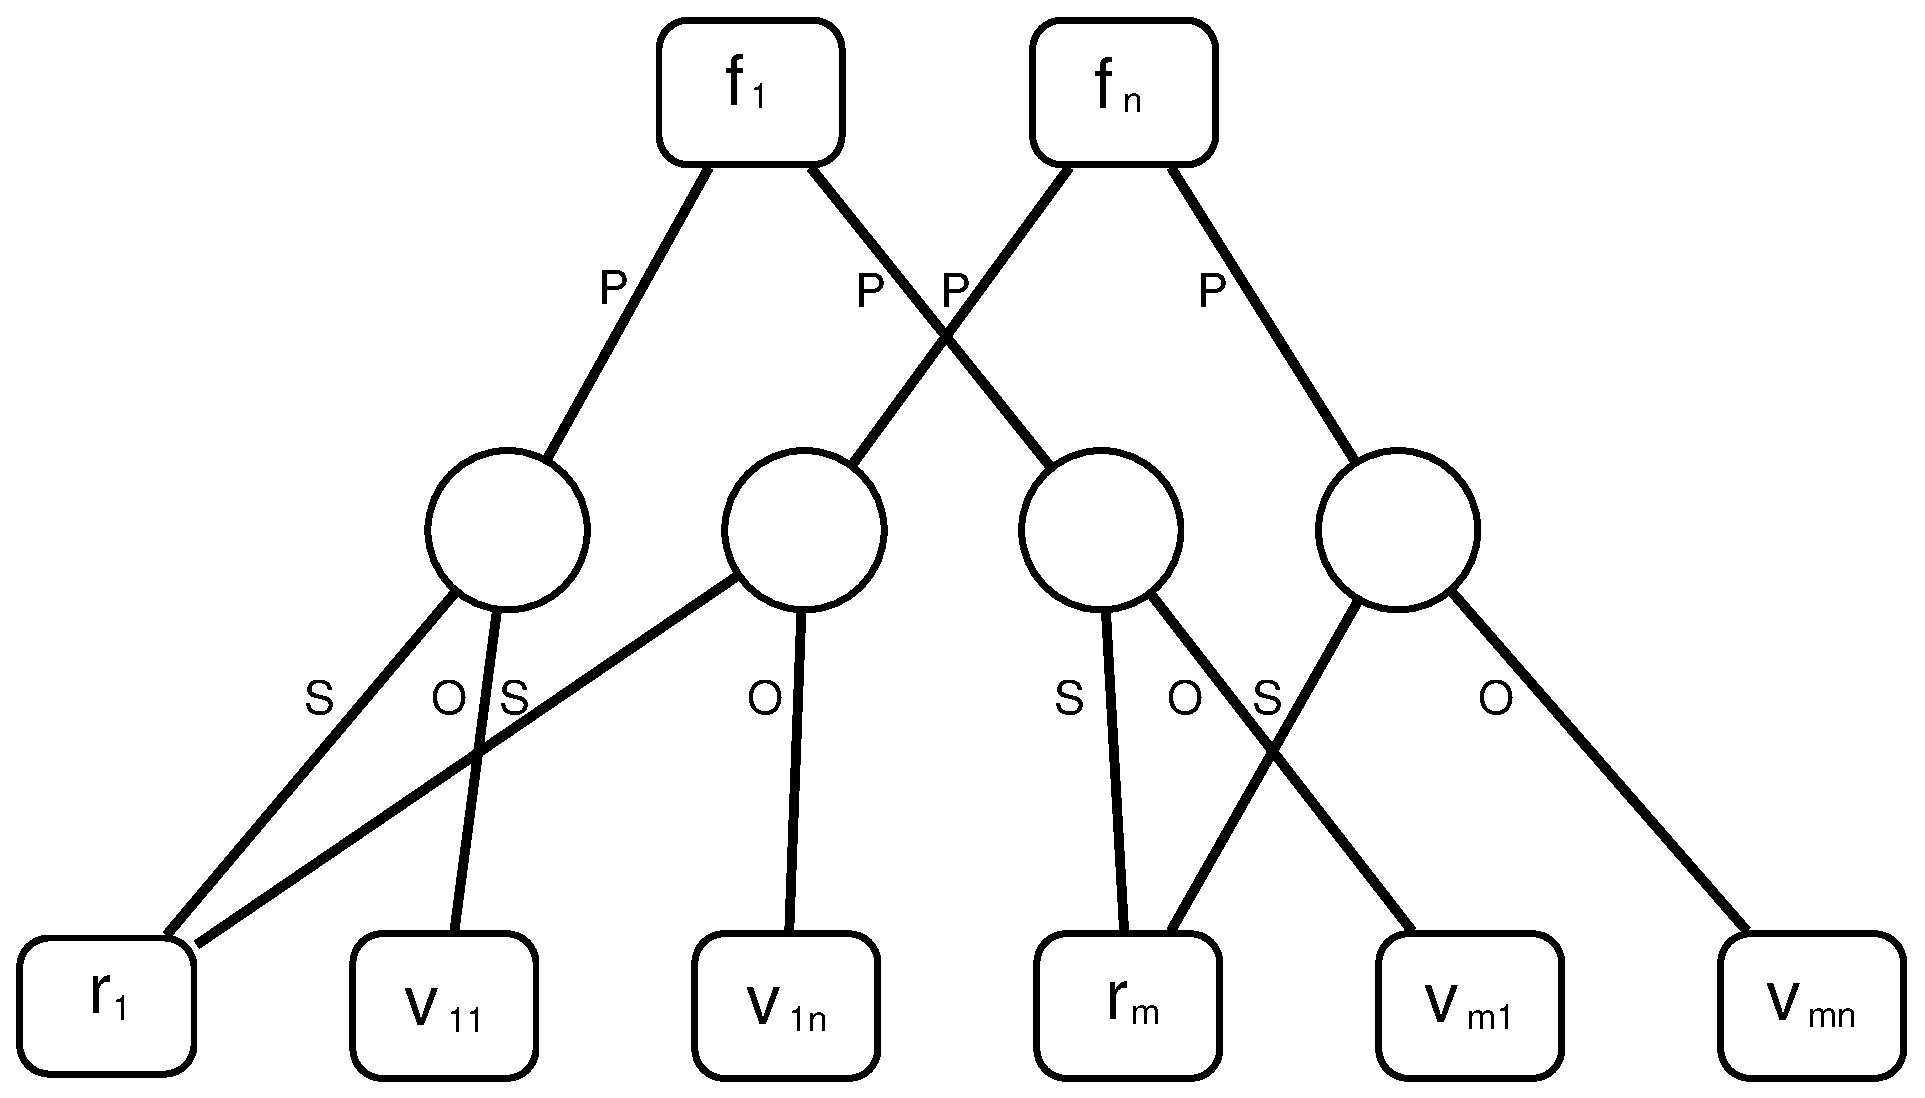
\includegraphics[width=.5\textwidth]{fig/BG-relational-nominal.eps}
\end{center}
\caption[The RDF bipartite graph for a nominal-valued table]{\label{fig:BG-relational-nominal} The RDF bipartite graph based on RDF triples in Table~\ref{tbl:nominal-rel} (B).}
\end{figure}

For relational tables with binary (boolean) features, the RDF representation can be more compact. In some applications, only cells with positive (``1") values are of interest. In this case, an auxiliary predicate can be introduced to link a row and positive cell values in that row.

\begin{myexp}[\textbf{RDF bipartite graph for a binary-valued RDB with positive values}]
\label{exp:repBinRDB}
Table~\ref{tbl:binary-rel} (A) shows an $m$-by-$n$ relational table with binary features. We use an auxiliary predicate \texttt{<mentions>} to denote a positive occurrence of a feature in one row, e.g., the statement \texttt{<$r_1$> <mentions> <$f_n$>} corresponds to the value ``1" in the $n$-th feature in the first row. Consequently, the whole Table~\ref{tbl:binary-rel} (A) maps to only two RDF statements in Table~\ref{tbl:binary-rel} (B).
\end{myexp}


\begin{table}[ht]
\begin{minipage}[b]{0.38\linewidth}\begin{flushright}
\begin{tabular}{ c | c | c | c |}
\cline{2-4}
	~   & $f_1$	    & $\cdots$  & $f_n$   \\
\cline{2-4}
$r_1:$	&  0  	& $\cdots$   &    1  \\
\cline{2-4}
$\vdots$& $\vdots$  & $\ddots$  & $\vdots$\\
\cline{2-4}
$r_m:$	&  1  	& $\cdots$   &    0  \\
\cline{2-4}
\end{tabular}
\end{flushright}
\end{minipage}
\hfill
\begin{minipage}[b]{0.4\linewidth}
\begin{tabular}{c c c}
\emph{s}&   \emph{p}&  \emph{o}\\
\texttt{<$r_1$>}   &    \texttt{<mentions>}   &  \texttt{<$f_n$>}\\
\texttt{<$r_m$>}   &    \texttt{<mentions>}   &  \texttt{<$f_1$>}\\
\end{tabular}
\end{minipage}
\begin{minipage}[c]{0.4\linewidth}\centering
\vspace{0.2cm}\hspace{2.8cm}(A)
\end{minipage}
\begin{minipage}[c]{0.4\linewidth}\centering
\vspace{0.2cm}\hspace{3.5cm}(B)
\end{minipage}
\caption{\label{tbl:binary-rel} An example relational table with binary features.}
\end{table}

Using the auxiliary predicate (\texttt{<mentions>}) greatly simplifies the resulting RDF graph by reducing the number of distinct predicates from $n$, according to the process in Definition~\ref{auto-map}, to only 1. This has profound implications for developing efficient analysis and mining methods based on the RDF bipartite graph.

However, the auxiliary predicate is feasible only when linking a row node with its positive value nodes in a binary-valued scenario. If negative cell values are also of interest and needs to be included in the RDF graph, the trick shown in the following example can be performed so that we can still use a single auxiliary predicate to link both positive and negative values:

\begin{myexp}[\textbf{RDF bipartite graph for a binary-valued RDB with both positive and negative values}]
\label{binary-reverse}
Table~\ref{tbl:binary-rel-expansion} (A) is derived from Table~\ref{tbl:binary-rel} (A) by adding a reverse column for each of its original columns, i.e., for each $f_i$, $i \in [1, n]$, a reverse $f_i'$ is created where $\forall{k\in[1,m]}~,~ v_{ki} = \neg v_{ki'}$. In this way, we can use the auxiliary predicate \texttt{<mentions>} to link to negative values by using the reverse column, because, for example, \texttt{<$r_1$> <mentions> <$f_1'$>} is equivalent to asserting $\neg$(\texttt{<$r_1$> <mentions> <$f_1$>})~. Table~\ref{tbl:binary-rel-expansion} (B) shows the RDF statements based on Table~\ref{tbl:binary-rel-expansion} (A) which essentially captures information of both positive and negative values from Table~\ref{tbl:binary-rel} (A).
\end{myexp}

\begin{table}[ht]
\begin{minipage}[b]{0.4\linewidth}\begin{flushright}
\begin{tabular}{ c | c | c | c | c | c |}
\cline{2-6}
	~   & $f_1$	 &  $f_1'$  & $\cdots$  & $f_n$  &  $f_n'$ \\
\cline{2-6}
$r_1:$	&  0  &  1	& $\cdots$   &    1  & 0\\
\cline{2-6}
$\vdots$& $\vdots$ & $\vdots$  & $\ddots$  & $\vdots$ & $\vdots$\\
\cline{2-6}
$r_m:$	&  1  &  0	& $\cdots$   &    0  & 1\\
\cline{2-6}
\end{tabular}
\end{flushright}
\end{minipage}
\hfill
\begin{minipage}[b]{0.4\linewidth}
\begin{tabular}{c c c}
\emph{s}&   \emph{p}&  \emph{o}\\
\texttt{<$r_1$>}   &    \texttt{<mentions>}   &  \texttt{<$f_1'$>}\\
\texttt{<$r_1$>}   &    \texttt{<mentions>}   &  \texttt{<$f_n$>}\\
\texttt{<$r_m$>}   &    \texttt{<mentions>}   &  \texttt{<$f_1$>}\\
\texttt{<$r_m$>}   &    \texttt{<mentions>}   &  \texttt{<$f_n'$>}\\
\end{tabular}
\end{minipage}
\hspace{1.5cm}
\begin{minipage}[c]{0.4\linewidth}\centering
\vspace{0.2cm}\hspace{2.8cm}(A)
\end{minipage}
\begin{minipage}[c]{0.4\linewidth}\centering
\vspace{0.2cm}\hspace{3.5cm}(B)
\end{minipage}
\caption{\label{tbl:binary-rel-expansion} An example expanded relational table with binary features.}
\end{table}

The process of adding reverse columns to binary-valued RDB tables described in Example~\ref{binary-reverse} can be extended to nominal-valued tables as well. By doing this we can achieve the desirable property of having only one predicate in the resulting RDF graph. The process is called RDB nominal value expansion as defined below.

\begin{mydef}[\textbf{RDB nominal value expansion}]
\label{nominal-expansion}
In a nominal valued RDB table, for each feature $f_i$ taking values on the set $V_i=\{v_{i1}, v_{i2}, \ldots\}$, we define $|f_i|$ to denote the number of its distinct values, i.e. $|f_i|=|V_i|$. The RDB nominal value expansion process transforms each nominal feature $f_i$ to $|f_i|$ number of binary features ($f_{i1}, f_{i2}, \ldots, f_{i|f_i|}$). The value of $k$-th row in $f_{ij}, (j\in [1, |f_i|)$, is ``1", if and only if $f_i$ takes the value $v_{ij}$ in the $k$-th row.
\end{mydef}

\begin{myexp}[\textbf{RDB nominal value expansion}]
Table~\ref{tbl:nominal-rel-expansion} (A) shows an nominal-valued RDB table with concrete column names and values. We use the formula, Outlook=\{sunny, overcast, rainy\}, to denote the set of distinct values the feature ``Outlook" can take on. Similarly, we have Temperature=\{hot, mild, cool\}, and Humidity=\{high, low\}. Table~\ref{tbl:nominal-rel-expansion} (B) shows the resulting table after nominal value expansion based on Definition~\ref{nominal-expansion}, and based on which, we derive the RDF statements all using one single auxiliary predicate \texttt{<mentions>}, as partly shown in Table~\ref{tbl:nominal-rel-expansion} (C).
\end{myexp}

\begin{table}[ht]
\begin{minipage}[b]{0.35\linewidth}
\begin{tabular}{ c | c | c | c |}
\cline{2-4}
	~   & O	    & T  & H   \\
\cline{2-4}
$r_1:$	&    sunny & hot & high  \\
\cline{2-4}
$r_2$:  &   rainy  & cool  & low\\
\cline{2-4}
$\vdots$& \multicolumn{3}{c|}{$\vdots$}\\
\cline{2-4}
$r_m:$	&  overcast  	& mild   & low  \\
\cline{2-4}
\end{tabular}
\end{minipage}
\begin{minipage}[b]{0.55\linewidth}
\begin{tabular}{ c | c | c | c || c | c | c || c | c |}
\cline{2-9}
~     & O\_s & O\_o & O\_r & T\_h & T\_m & T\_c & H\_h & H\_l \\
\cline{2-9}
$r_1:$ & 1 & 0 & 0 & 1 & 0 & 0 & 1 & 0 \\
\cline{2-9}
$r_2:$ & 0 & 0 & 1 & 0 & 0 & 1 & 0 & 1 \\
\cline{2-9}
$\vdots$& \multicolumn{8}{c|}{$\vdots$}\\
\cline{2-9}
$r_m:$ & 0 & 1 & 0 & 0 & 1 & 0 & 0 & 1 \\
\cline{2-9}
\end{tabular}
\end{minipage}
\hspace{1.5cm}
\begin{minipage}[c]{0.35\linewidth}\centering
\vspace{0.2cm}\hspace{1.5cm}(A)
\end{minipage}
\begin{minipage}[c]{0.55\linewidth}\centering
\vspace{0.2cm}\hspace{1.5cm}(B)
\end{minipage}
\begin{minipage}[b]{\linewidth}\centering
\begin{tabular}{c c c}
&&\\
\emph{s}&   \emph{p}&  \emph{o}\\
\texttt{<$r_1$>}   &    \texttt{<mentions>}   &  \texttt{<O\_s>}\\
\texttt{<$r_1$>}   &    \texttt{<mentions>}   &  \texttt{<T\_h>}\\
\texttt{<$r_1$>}   &    \texttt{<mentions>}   &  \texttt{<H\_h>}\\
\texttt{<$r_2$>}   &    \texttt{<mentions>}   &  \texttt{<O\_r>}\\
\multicolumn{3}{c}{$\cdots$}\\
\multicolumn{3}{c}{(C)}\\
\end{tabular}
\end{minipage}
\caption[Nominal value expansion for a relational table and the resulting RDF triples.]{\label{tbl:nominal-rel-expansion} An example nominal-valued relational table after nominal value expansion. (A) shows the original table where O stands for ``outlook", T for ``temperature" and "H" for humidity. (B) shows the expanded table. (C) shows the corresponding RDF triples derived from (B).}
\end{table}

\section{Combining Data Graphs and Ontology Graphs}

In order to seamlessly interface data and domain knowledge in a mining framework, the information in both sources needs to be first associated. This is achieved by the process called \emph{semantic annotation}. Semantic Annotation aims at assigning to the basic element of data links to formal semantic descriptions. Such elements should constitute the semantics of their source, for example, named entities in a document, certain part of an image depicting someone's head portrait.

Semantic annotation is crucial in realizing semantic data mining by bridging formal semantics in domain knowledge with data. What is more important, semantic annotation also enables a spectrum of new applications, such as indexing, retrieval, inference, categorization, query answering etc. These applications can also play vital roles in semantic data mining.

In the following, we assume data is annotated, meaning the links between entities in the data and formal semantic descriptions (such as those in ontologies) are established. A unified graph incorporating information from both data and domain knowledge can be created. Data mining algorithms dealing with such graph enjoys the benefits of a seamless integration of domain semantics. The following example shows the combination of an ontology graph and a data graph.

%\textbf{b) Domain Semantics--driven Mapping Generation}: The second approach generates mappings from RDB to RDF by incorporating domain semantics that is often implicit or not captured at all in the RDB schema. The explicit modeling of domain semantics, often modeled as a domain ontology. The domain ontology may be pre--existing and sourced from public resources.

\begin{myexp}[\textbf{Combining an ontology graph and a data graph}]
Figure~\ref{fig:onto-and-data} (A) shows an simple ontology in some domain with only subsumption relationship defined for five entities (A--B). Figure~\ref{fig:onto-and-data} (B) shows a binary-valued RDB table in the same domain with the set of entities serving as features. We use the same entity labels in the ontology and the RDB table because we assume the mapping between ontology nodes and table features are pre-assigned or established by automatic annotation. Figure~\ref{fig:hypergraph-combined} (B) shows the RDF statements derived from both the ontology and the RDB table. Figure~\ref{fig:hypergraph-combined} (A) demonstrates the combined RDF bipartite graph.

Positions of nodes in Figure~\ref{fig:hypergraph-combined} (A) can be rearranged to form Figure~\ref{fig:bipartitegraph-weighted}. This graph demonstrates a tripartite structure where row nodes ($r_1$--$r_5$) fall on one partition, column nodes (A--E) another, and statement nodes in between. A plethora of graph-theoretic algorithms and graph mining techniques can be leveraged to analyze the configuration of connecting paths in this graph to answer questions such as grouping in rows and columns (for solving the the task of clustering and association mining respectively). Predicate nodes can serve as a sign to introduce different weights to paths in order to distinguish different semantic information conveyed by those predicates.

Edges and statement nodes in Figure~\ref{fig:bipartitegraph-weighted} are depicted in two colors to signify their sources of origin. Red edges and nodes denote information from the data (RDB table), and blue ones from the ontology. It can be seen from the graph that the contribution of ontology is to introduce extra paths with different semantic types (The data is structured under the ``mentions" relationship and the ontology is structured under the subsumption relationship). A mining algorithm that is able to deal with the data graph can be naturally extended without major modification to handle domain knowledge coded in the ontology.
\end{myexp}

\begin{figure}[tbh]
\begin{minipage}[c]{.45\textwidth}\centering
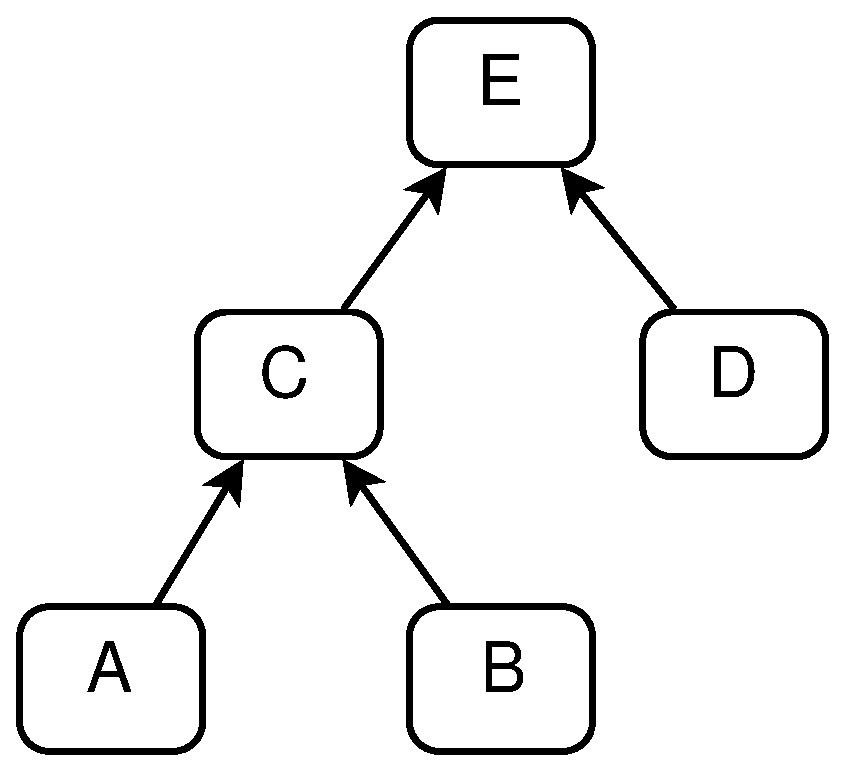
\includegraphics[width=.5\linewidth]{fig/simple-onto.eps}
\end{minipage}
\begin{minipage}[b]{.45\textwidth}\centering
    \begin{tabular}{ c | c | c | c | c | c |}
    \cline{2-6}
    	~ & A & B & C & D & E\\
    \cline{2-6}
    $r_1:$& 1 & 1 & 0 & 0 & 0 \\
    \cline{2-6}
    $r_2:$& 1 & 1 & 1 & 0 & 0 \\
    \cline{2-6}
    $r_3:$& 0 & 1 & 1 & 0 & 0 \\
    \cline{2-6}
    $r_3:$& 0 & 0 & 0 & 1 & 0 \\
    \cline{2-6}
    \end{tabular}
\end{minipage}
\begin{minipage}[c]{0.4\linewidth}\centering
\vspace{0.2cm}\hspace{2cm}(A)
\end{minipage}
\begin{minipage}[c]{0.4\linewidth}\centering
\vspace{0.2cm}\hspace{4cm}(B)
\end{minipage}
\caption[A example relational table and a domain ontology]{\label{fig:onto-and-data} An example of a binary-valued relational table (B) about five concepts (``A"--``E"), and the ontological relationship among these concepts shown as a directed graph (A).}
\end{figure}

\begin{figure}[tbh]
\begin{center}
\begin{tabular}{c  c}
\multirow{12}{*}{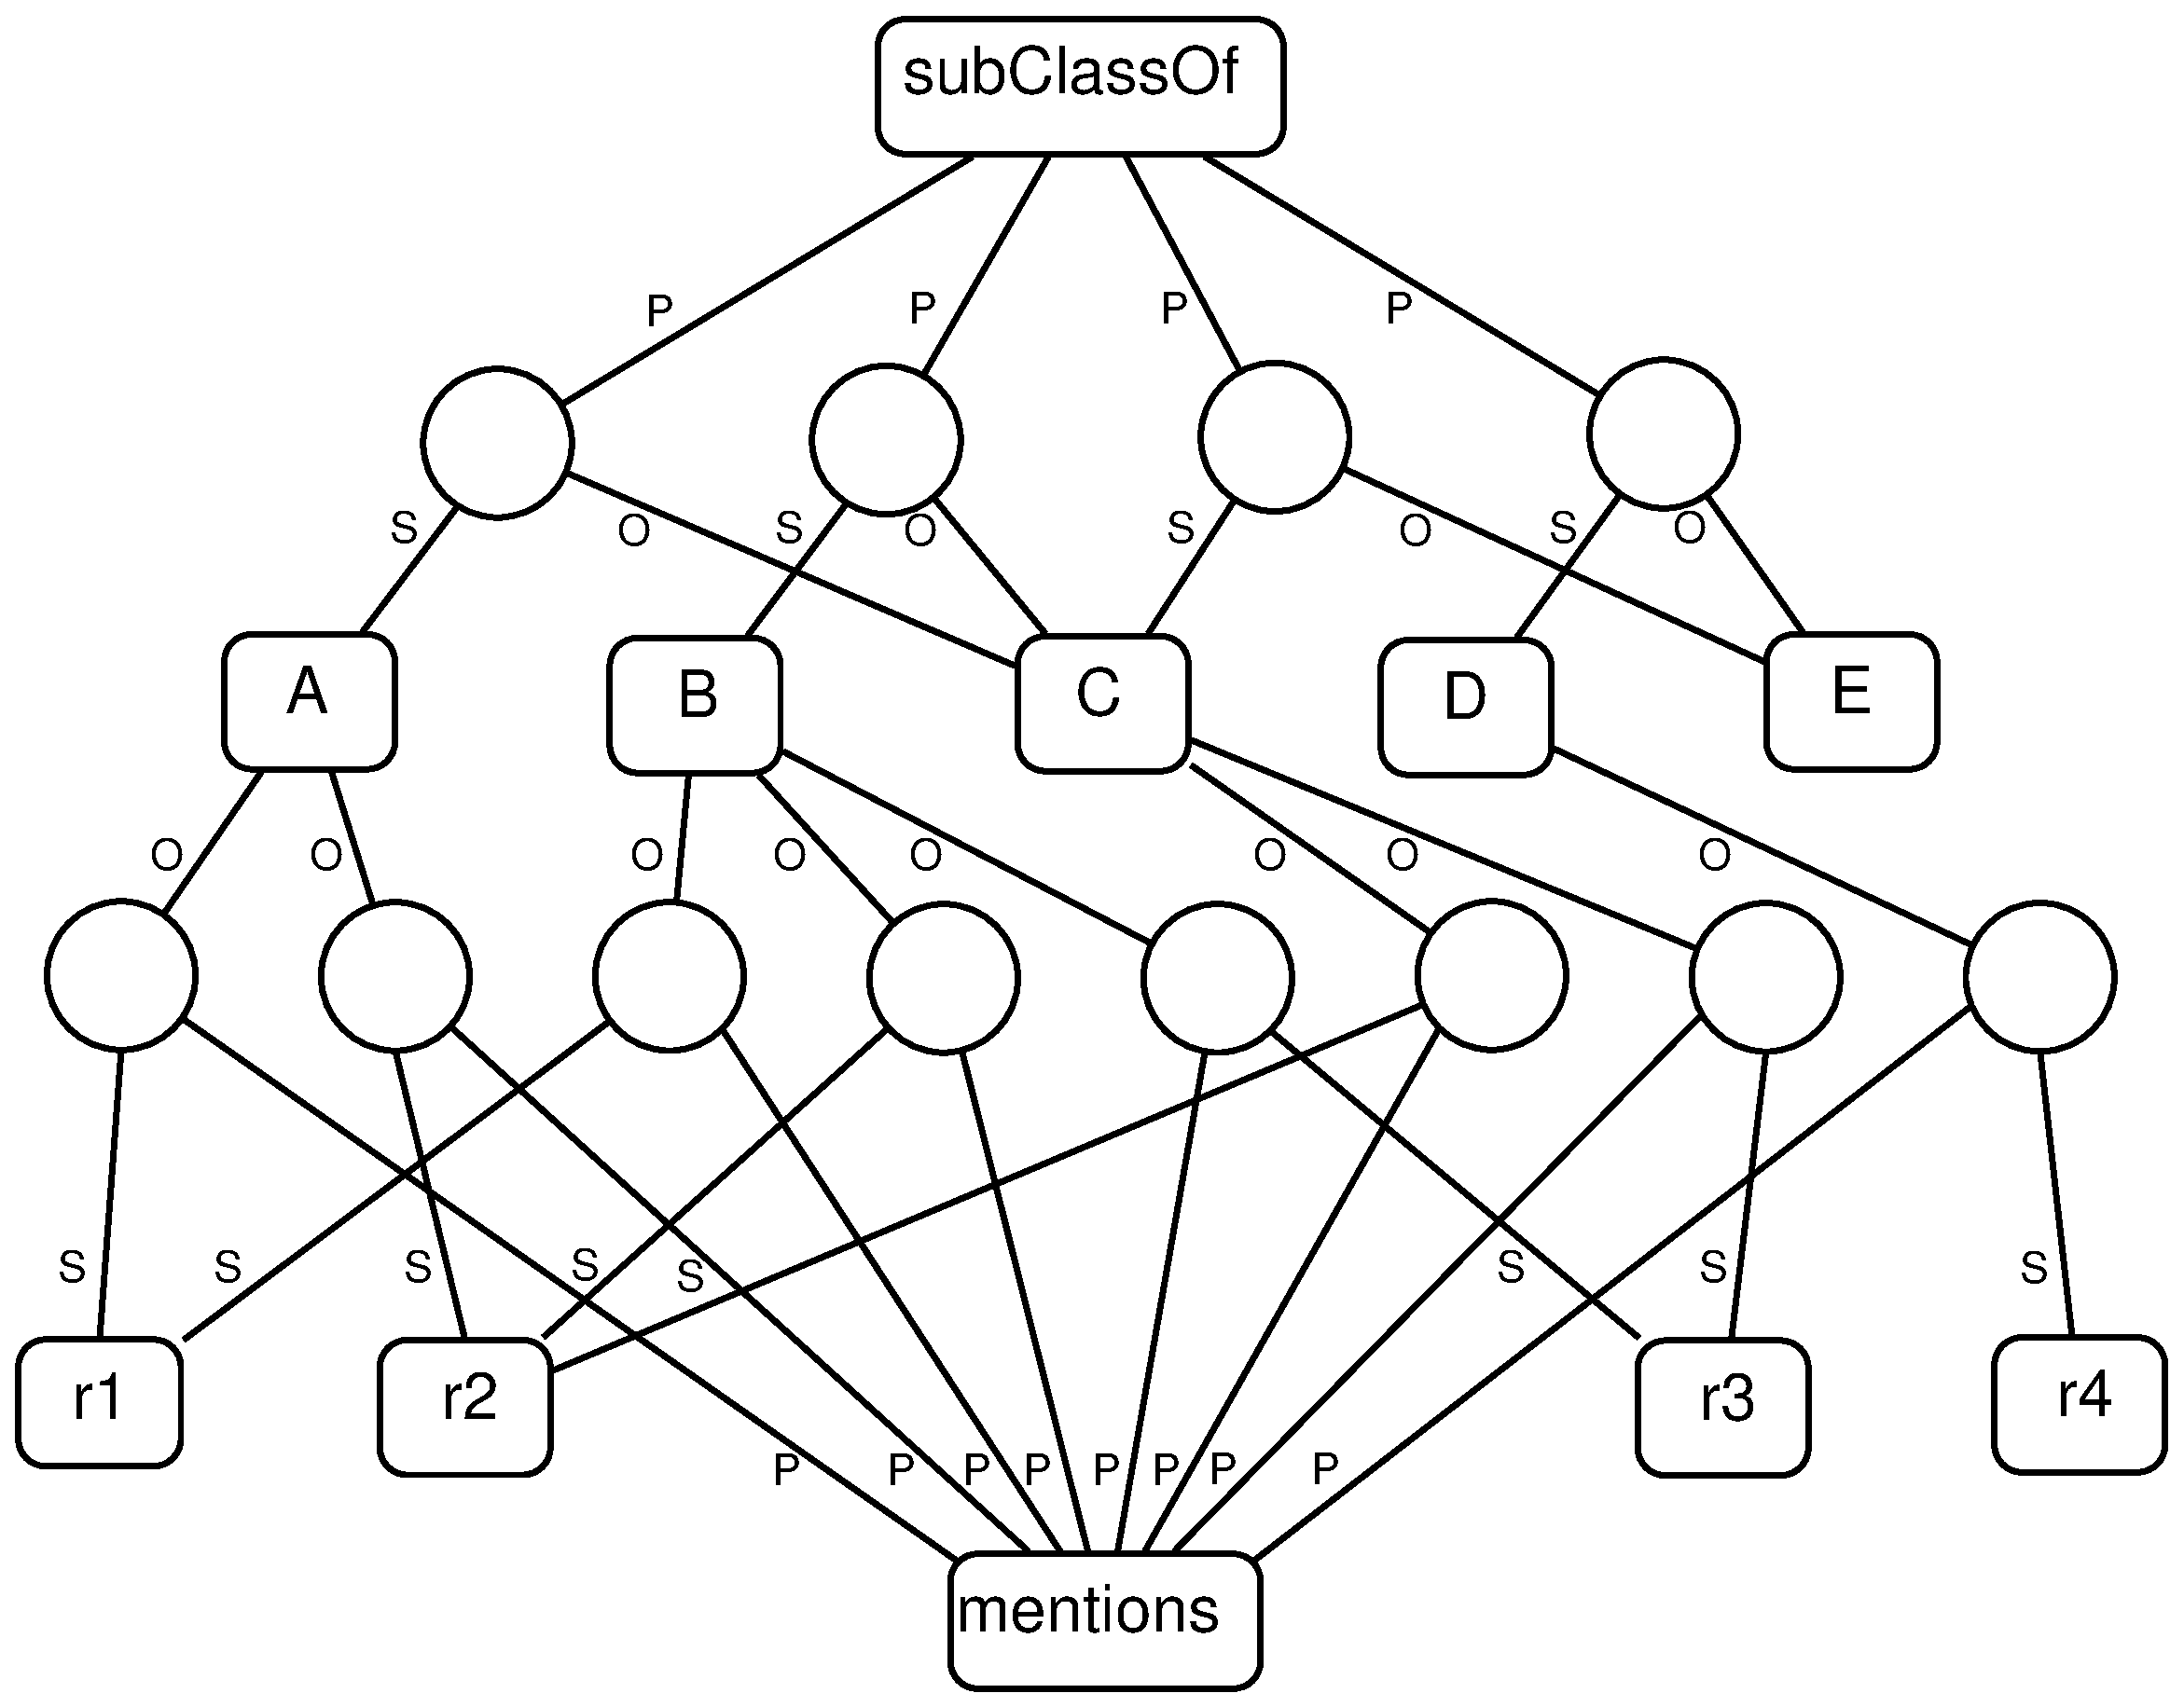
\includegraphics[width=.55\textwidth]{fig/hypergraph_mining.eps}} & \emph{~~~s \hfill p\hfill o~~~}\\
& \texttt{<A>~~<subClassOf>~~<C>}\\
& \texttt{<B>~~<subClassOf>~~<C>}\\
& \texttt{<C>~~<subClassOf>~~<E>}\\
& \texttt{<D>~~<subClassOf>~~<E>}\\
& \\
& \texttt{<r1>\;~~<mentions>\;~~<A>}\\
& \texttt{<r1>\;~~<mentions>\;~~<B>}\\
& \texttt{<r2>\;~~<mentions>\;~~<A>}\\
& \texttt{<r2>\;~~<mentions>\;~~<B>}\\
& \texttt{<r2>\;~~<mentions>\;~~<C>}\\
& \texttt{<r3>\;~~<mentions>\;~~<B>}\\
& \texttt{<r3>\;~~<mentions>\;~~<C>}\\
& \texttt{<r4>\;~~<mentions>\;~~<D>}\\
& \\
& \\
(A) & (B)\\
\end{tabular}
\end{center}
\caption[The RDF bipartite graph as the combined representation]{\label{fig:hypergraph-combined} The RDF bipartite graph representation (A) given triples shown in (B) based on the information described in Figure~\ref{fig:onto-and-data}.}
\end{figure}

\begin{figure}[tbh]
\begin{center}
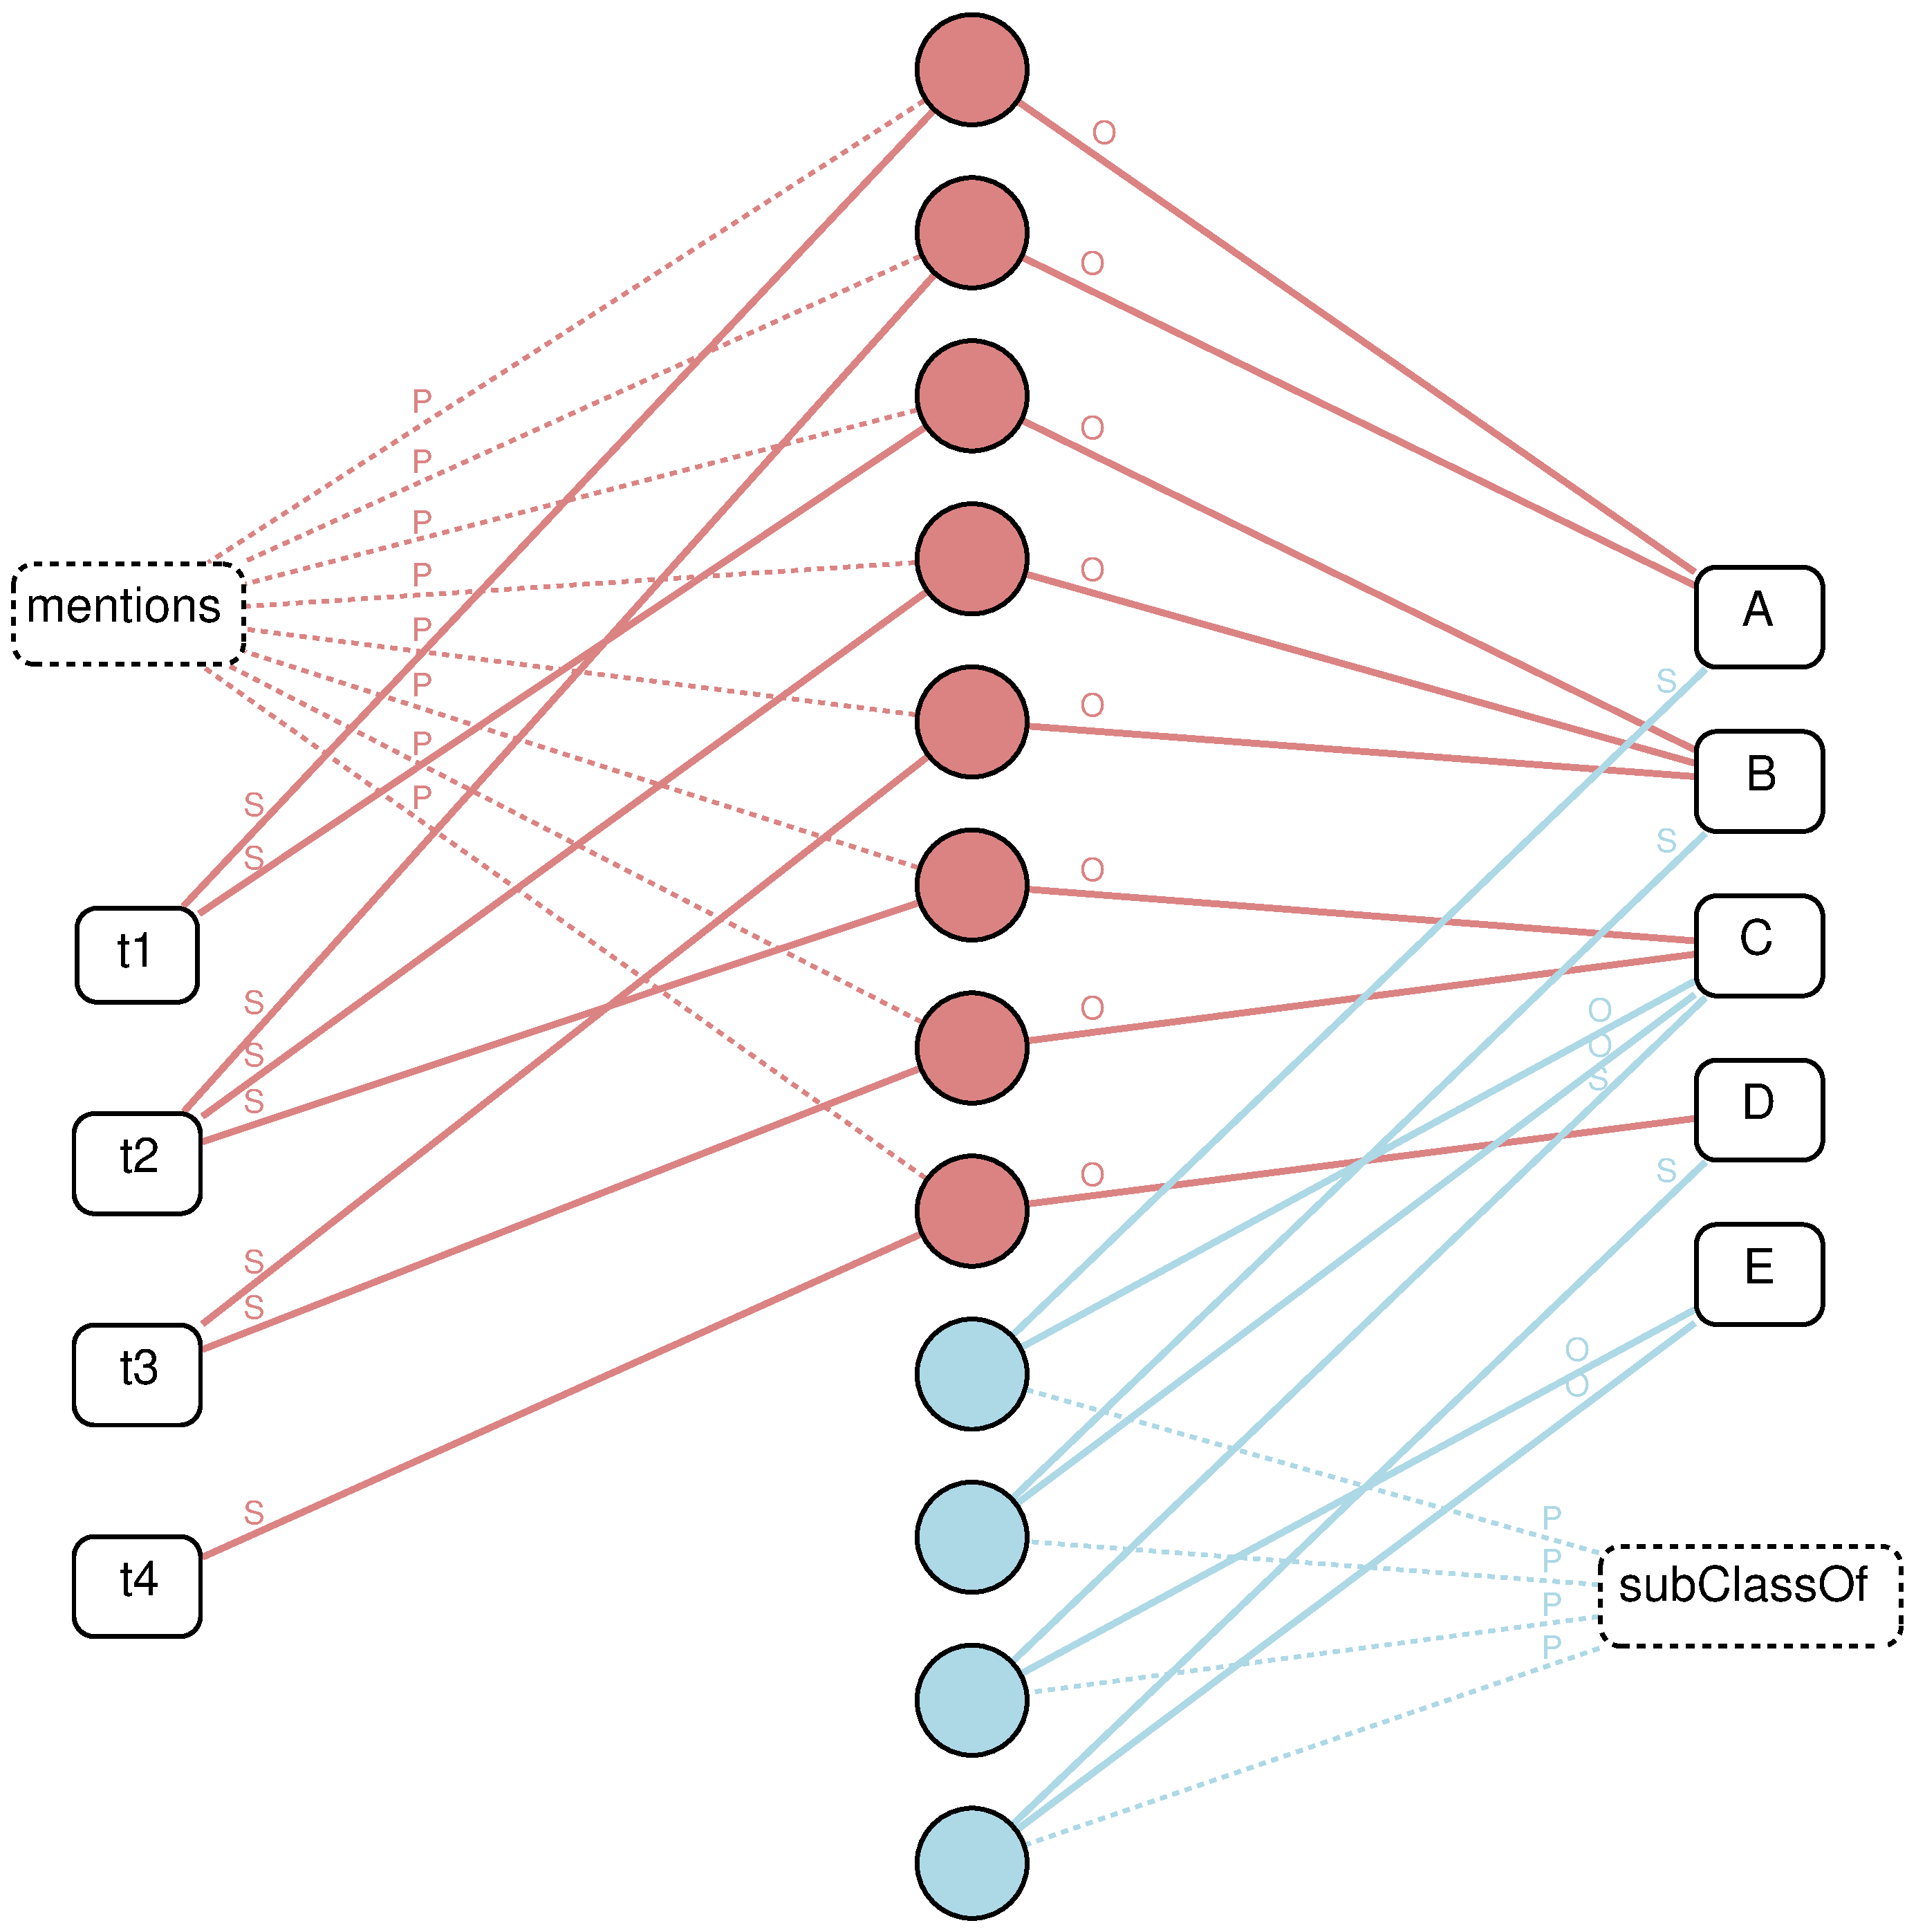
\includegraphics[width=.6\textwidth]{fig/hypergraph_mining-bipartite-weighted.eps}
\end{center}
\caption[Transforming the RDF bipartite graph to suit mining need]{\label{fig:bipartitegraph-weighted} This figure shows that, grouping the nodes according to whether they are row elements or column elements in Figure~\ref{fig:onto-and-data} (B), the bipartite graph shown in Figure~\ref{fig:hypergraph-combined} (A) can be further transformed to a tripartite graph.}
\end{figure}

\subsection{Representing Different Kinds of Ontological Semantics}
\label{sec:rosg}

%In our preliminary work, we have showed a way to represent ontology annotated data in hypergraphs which help discovering semantic associations.  If the domain knowledge is defined as formal ontologies, it is a natural thinking to use graphs to represent the domain knowledge as well. To formally represent domain knowledge using graphs, it is important to different types of formal semantics in a systematic way.

In order to leverage the increasingly larger and richer collection of domain ontologies, especially in scientific fields such as the biomedical domain, we propose to develop methods for the representation of different types of ontological semantics which supports efficient semantic data mining. We propose to develop a weighting scheme to distinguish paths in the RDF bipartite graph that contains these different relationships such as class subsumption, part\_of, and other general or domain--specific properties. %(e.g., Drug \textit{treat} Disease).

\begin{myexp}[\textbf{Assigning weights to different relationship}]
Figure~\ref{fig:hypergraph_mining-comp} shows an example of RDF bipartite graph representing information on peoples (A--E) where multiple relationships can be identified to link them. E.g., A, B, C and D are linked by the coauthorship relationship, while D and E are linked by the more general collaboration relationship (in fact, coauthorship is defined as a sub-property of collaboration in the ontology). A, B and C are professors, D and E are PhD students, and both professors and PhD students are researchers. In this complex lattice of relationships, we hope to distinguish these relationships by assigning task--specific weights to the related paths (e.g., as conveyed by different colorings in the graph). In order to achieve this, we propose to develop a framework for guiding the (semi-) automatic assignment of weights.
\end{myexp}

\begin{figure}[tbh]
\begin{center}
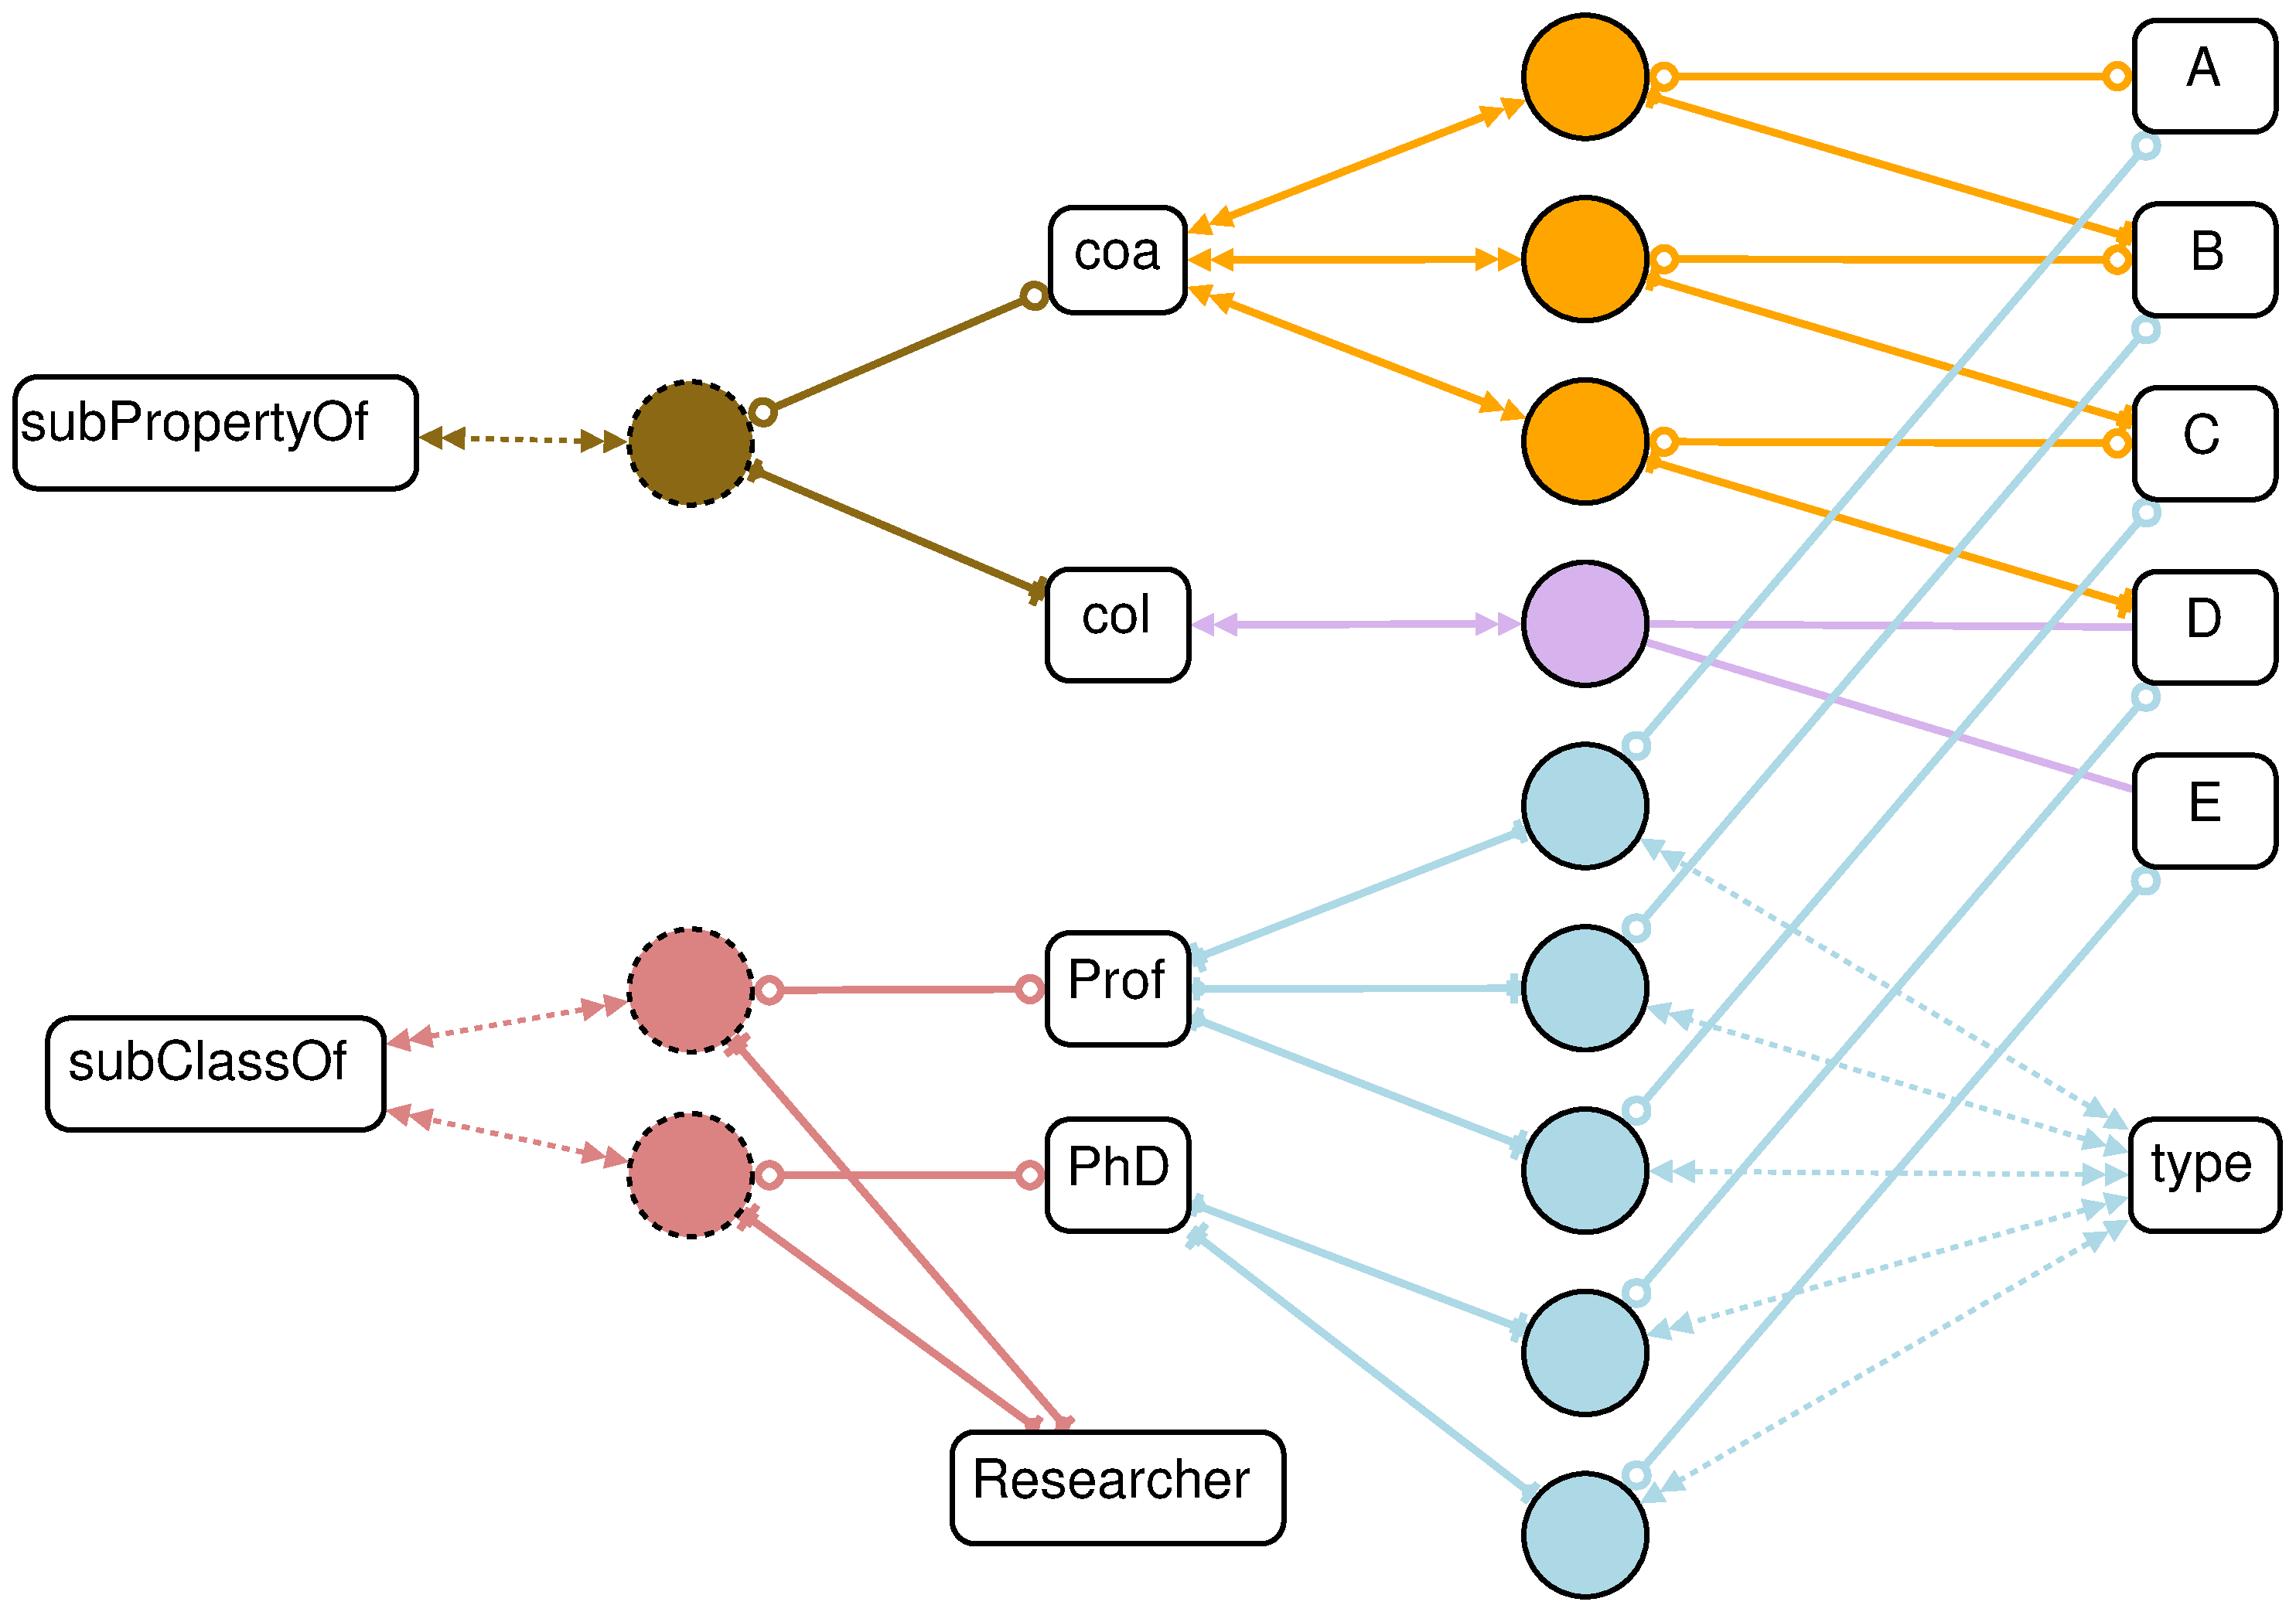
\includegraphics[width=.65\textwidth]{fig/hypergraph_mining-comp.eps}
\end{center}
\caption[An example RDF bipartite graph that represents various semantic relationships]{\label{fig:hypergraph_mining-comp} An example RDF bipartite graph that represents various semantic relationships.}
\end{figure}


%%%%%%%%%%%%%%%%%%%%%%%%%%%%%%%%%%%%%%%%%%%%%%%%%%%%%%%%%%%%%%%%%%%

\chapter{SEMANTIC ANNOTATION}
\label{chap:annotation}
Annotation in general (traditionally) is a summary made of information in some source such as document, online record, image, video and so forth. With the emergence and development of the Semantic Web, there have been increasing demands for \emph{semantic annotation}, a kind of meta-data derived based upon specific knowledge about the world, rather than indifferent to any ontological commitments. In other words, semantic annotation aims at assigning to the basic element of information links to formal semantic descriptions~\cite{KiryakovEtal04}. Such elements should constitute the semantics of their source, for example, named entities in a document, certain part of an image depicting someone's head portrait.

Semantic annotation is crucial in realizing semantic data mining by bridging formal semantics in Semantic Web meta-data with data. The majority of data underpinning a wide spectrum of data mining applications are stored in various formats, including structured sources such as relational databases (RDB) with their proven track record of scalability and reliability, or semi-structured sources such as spreadsheets with their advantage of low maintenance and cheaper overheads, or even unstructured sources such as text corpus. The problem of how to impart knowledge encoded in Semantic Web ontologies to all sorts of data becomes a major challenge in realizing the semantic data mining. We believe \emph{semantic annotation} is the solution to this challenge. It aims at assigning semantic descriptions to elements of data. To ease the burden of common users that are not familiar with the Semantic Web, we develop a learning-based semantic search algorithm to suggest appropriate semantic descriptions for annotation.

%thesis-semantic-annotation-workflow
\begin{figure}[tbh]
\begin{center}
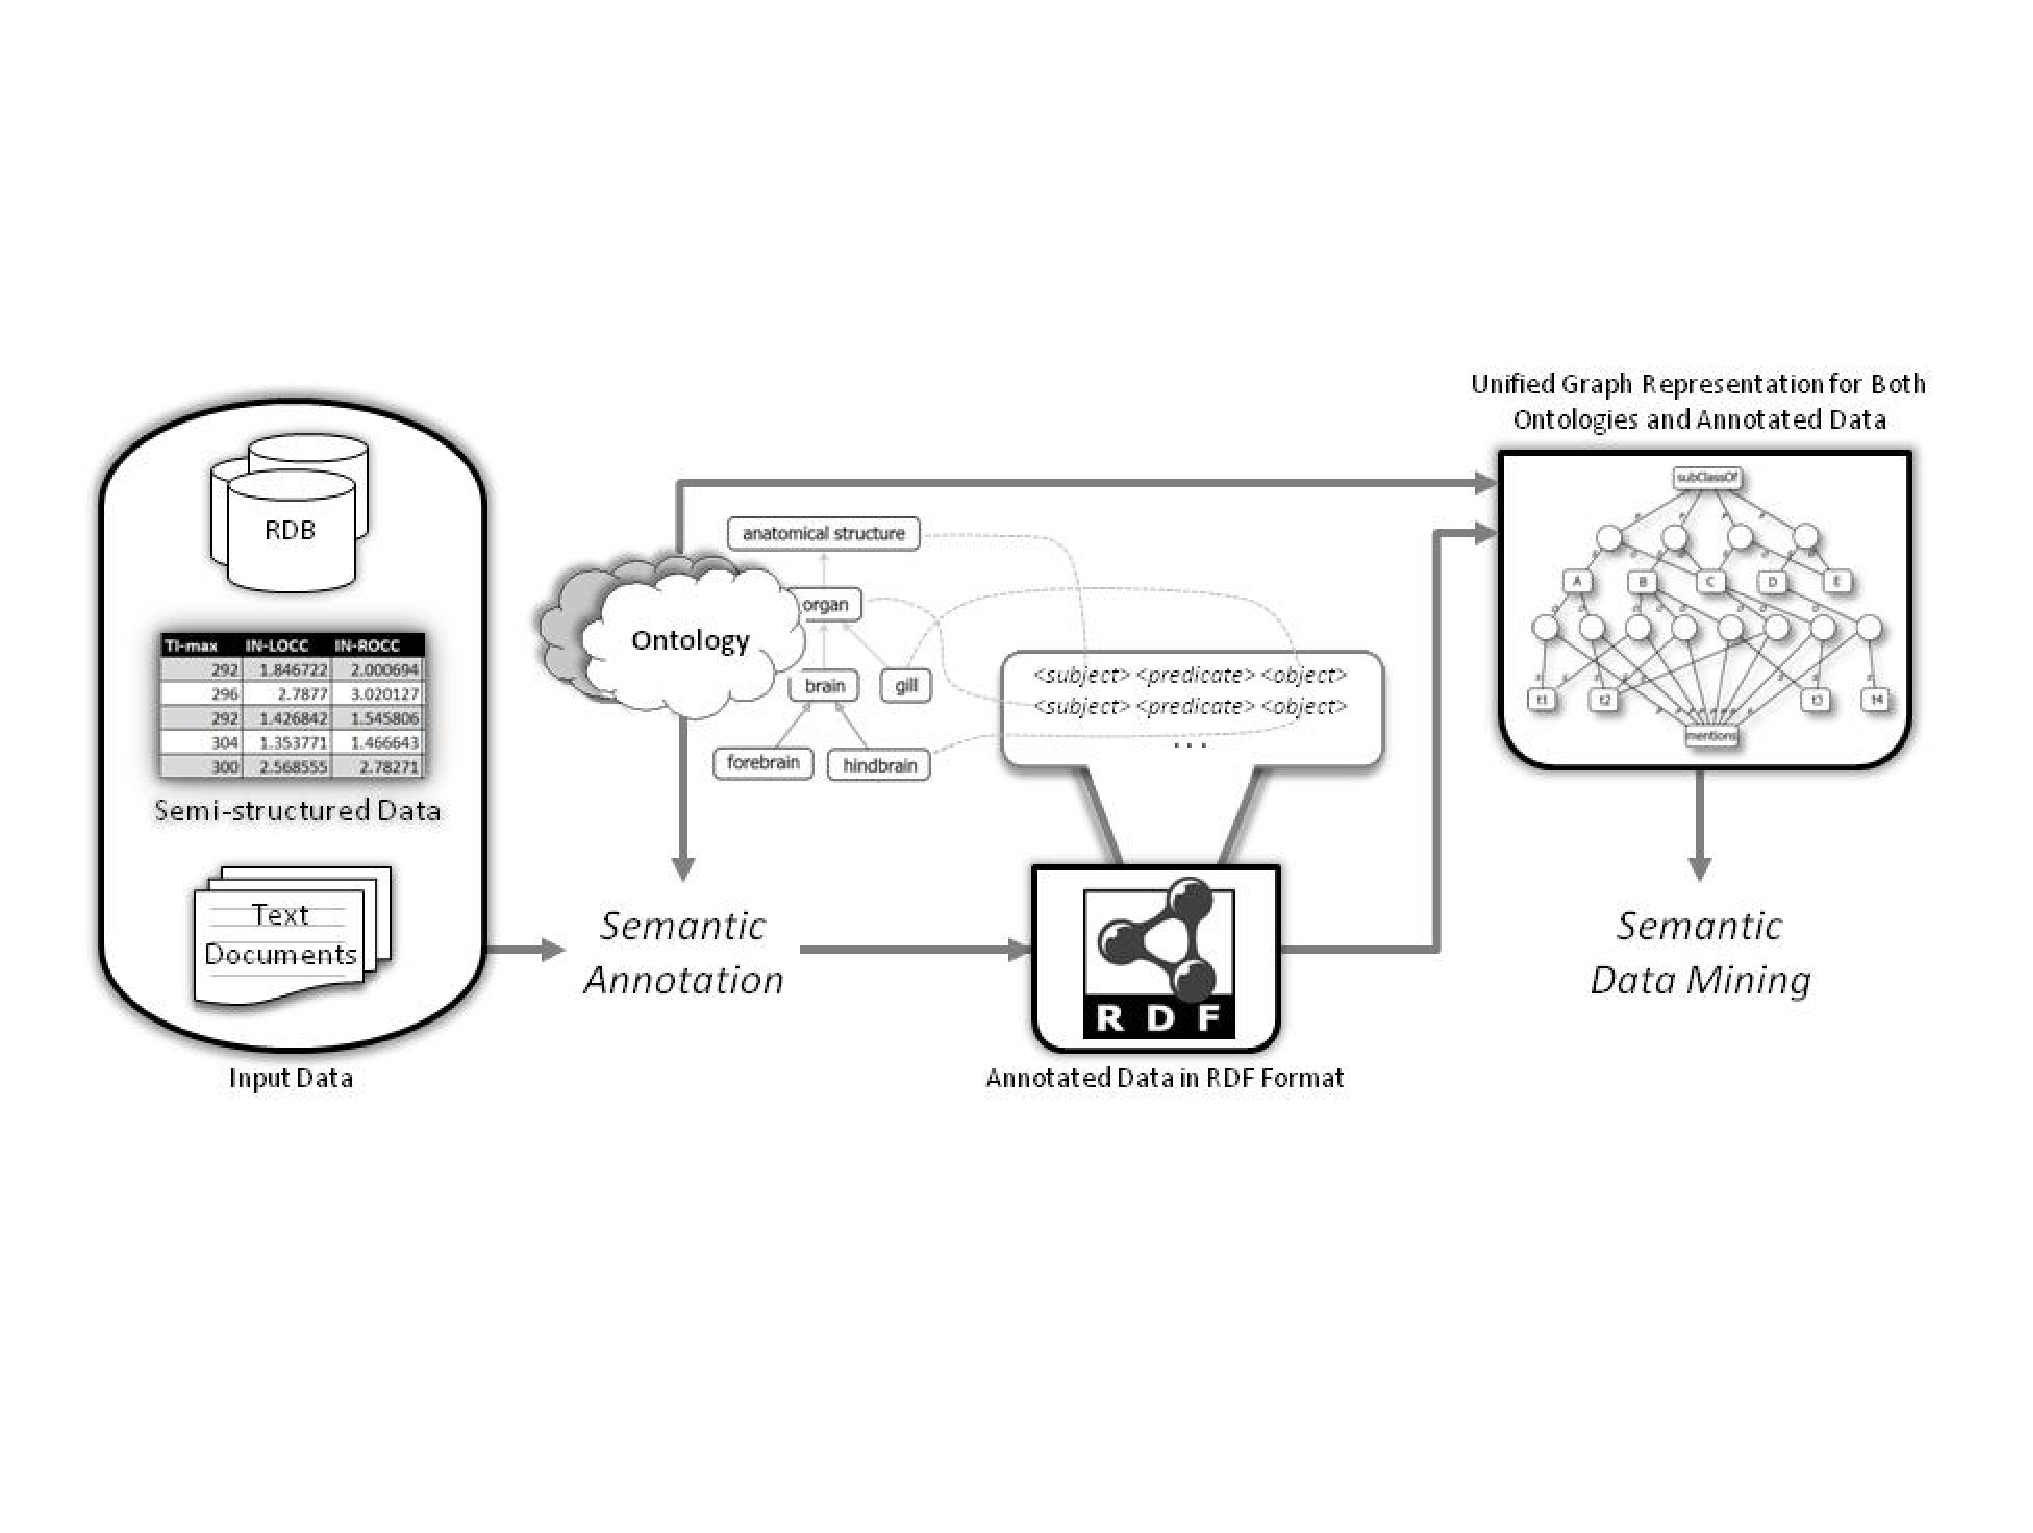
\includegraphics[width=\textwidth, trim=0 7cm 0 6cm, clip=true]{fig/thesis-semantic-annotation-workflow.eps}
\end{center}
\caption[Semantic annotation in the workflow of semantic data mining.]{\label{fig:annotation-workflow} Data stored in different sources (e.g., relational databases, spreadsheets, texts etc) are semantically annotated. The output is in RDF format where elements of data are linked to formal semantic descriptions in ontologies. Annotated data and ontologies together are then represented in a unified graph representation for subsequent analysis in semantic data mining.}
\end{figure}

\section{Automatic Annotation by Semantic Search}
Semantic annotation is crucial in realizing semantic data mining by bringing meanings to data. The function of semantic annotation in the workflow of a semantic data mining system is illustrated in Figure~\ref{fig:annotation-workflow} Annotating unstructured data (e.g., text) has been studied more extensively than annotating (semi-)structured data due to the proliferation of information extraction techniques that facilitate automatic entity recognition from text. Since large amount of data for knowledge discovery applications are stored in (semi-)structured sources, we focus on annotating (semi-)structured data.

The annotation process can be generally divided into two steps. The first is to establish mappings between existing Semantic Web terms and terms need to be annotated in the data. The second step is to come up with a local ontological structure constituting the semantic web terms to model the data.

Most of previous work in annotating (semi-)structured data focus on the second step. Some skip the first step and bootstrap the ontological terms and structure from the local data itself. For example, a number of systems that map data in RDB to RDF format leverage a set of rules such as ``table to class and column to predicate". Bernes-Lee expands the rule as follows~\cite{TBL98}: 1) An RDB record is a RDF node. 2) The column name of an RDB table is an RDF predicate. And 3) An RDB table cell is a value. Other examples of rules involved in mapping RDB schema to OWL ontology include ``foreign keys to object property and non-key attributes to datatype property".
Similar idea has been adopted in annotating spreadsheets as well. Existing spreadsheet-to-rdf tools typically map spreadsheets to star-shaped RDF graphs, i.e., each row is an instance, with each column representing a property. Some tools try to express richer spreadsheet semantics, e.g., Han et al. developed a spreadsheet-to-rdf tool called RDF123~\cite{RDF123} that allows users to define mappings to arbitrary graphs.

We argue that mapping RDB or spreadsheet to linked data (e.g., RDF) without referencing to existing semantic descriptions does not lend itself well to aiding semantic data mining. The automatically constructed self-contained local ontology may be applicable to describe a specific dataset but is most likely too rough to capture the full domain semantics that is necessary to express meaningful domain knowledge. Moreover, with the advent of the Semantic Web and pervasive connectivity, an increasing number of ontologies has been made widely available for reuse. These ontologies are created by thorough knowledge engineering process and should serve as better models for annotation. However, on the other hand, the sheer number of Semantic Web ontologies and lack of effective search functionality can lead to a huge hidden barrier for common users. Choosing proper Semantic Web ontologies and terms (classes and properties) requires familiarity with appropriate ontologies and the terms they define. There is very few system that is able to provide automatic suggestions. To solve this problem, we propose a learning-based semantic search algorithm to suggest proper Semantic Web terms and ontologies for annotation given semantically related words and general domain and context information.

In order to suggest suitable Semantic Web terms and ontologies for users to annotate their data, we propose a learning-based semantic search algorithm. We first submit a list of terms appeared in the schema of (semi-)structured data to our semantic search algorithm and then use the returned results for annotation. In a fully automatic setting, the search algorithm is configured to return the top-1 hit; while in an interactive setting, the search algorithm returns ordered top-k search results for users to decide. Previous semantic search algorithms leverage a variety of measures, including lexical and structural similarities (see details below) to rank Semantic Web documents according to how likely they can be semantically matched to the search terms. However, using any single measure alone may not be sufficient to achieve the optimal result. We propose to combine various measures to a weighted feature-based search model, where the weights are learned from training data. We believe the incorporation of learning techniques will improve the semantic search result. We have built a prototypical system for gathering training data for two algorithms: logistic regression and subgradient descent. The evaluation of such method is a matter of ongoing research.


\section{Matching Ontologies}
%%general review of the field of ontology matching
The presence of heterogeneity among schemas supporting vast amount of information demands advanced solution for semantic integration of disparate data sources to facilitate interoperability and reuse of the information. The challenge is especially pronounced in many scientific domains where a massive amount of data are produced independently and thus each having their own data vocabulary. While manual integration is time-consuming and requires expensive specialized human capital, the development of automatic approaches becomes imminent to aid inter-institute collaborations. One purpose is to suggest a method for solving a specific kind of ontology matching problem under some serious constraints that can cause traditional methods to be ineffective. The constraints that we deal with are, namely, 1) little-to-no string-based or linguistic similarity between terminologies, and 2) all numeric typed data instances. This phenomenon is commonly seen in integrating scientific datasets which involves discovery of correspondences among distinct numeric-typed summary features (``attributes") that are used to characterize datasets that have been collected and analyzed in different research labs. We call this the \emph{attribute matching} problem.

Another challenging task given multiple data sources is to carry out meaningful meta-analysis that combines results of several studies on different datasets to address a set of related research hypotheses. Finding correspondences among distinct patterns that are observed in different scientific datasets is an example of meta-analysis. Supposing the patterns are derived by clustering analysis, this problem can be addressed by the application of cluster comparison (or cluster matching) techniques. Clustering is an unsupervised data mining task widely used to discover patterns and relationships in a variety of fields. The clustering result provides a pattern characterization from a data-driven perspective. If similar results are obtained across multiple datasets, this leads in turn to a revision and refinement of existing domain knowledge, which is a central goal of meta-analysis. However, there are noticeably few cluster comparison methods that are able to compare two clusterings derived from different datasets. The difficulty for the comparison is further exacerbated by the fact that the datasets may be described by attributes from heterogeneous schemas or ontologies. Even those methods that are able to measure clustering similarity across different datasets (e.g., the ADCO~\cite{Bae2010} method) have to assume the homogeneous meta-data (e.g., the same schemas).

Given this situation, in order to carry out cluster comparison for meta-analysis, researchers often need to perform ontology or schema matching first in order to mitigate the gap for meta-data. In previous work~\cite{LiuEtal10}, we examine a practical attribute matching problem on neuroscience data where schema elements from one dataset share no lexical similarity with those from the other. Moreover, structural similarity is also limited. One can only resort to instance-based (extensional) methods. However, since all attributes are numerical, information clues available to an instance-level matcher is very restricted. Traditional instance-based matchers typically make use of constraint-based characterization, such as numerical value ranges and averages to determine correspondences. However, this is often too rough in the case of all-numerical dataset. Two attributes may have similar ranges and averages but totally different internal value distributions (an example is shown in Section~\ref{sec:syn_exp}). Given this, we propose to represent the attribute value distribution at a finer granularity by partitioning the values into groups. To do this, clustering is performed, and resulting clusters are then aligned across two datasets (assuming that the same pattern exists in both datasets). In this way, each attribute can be characterized by, instead of a single value, a vector of per-cluster statistical quantities (i.e., the \emph{segmented statistical characterization}). A distance function can then be applied based on this representation. Table~\ref{tbl:sim_mat}(A) shows an example distance table on the cross join of two sets of attributes. To discover attribute matching from this table can be reduced to solving a minimum assignment problem (assuming matching is bijective), which is a classical combinatory optimization problem that has a polynomial solution using the Hungarian Method~\cite{Kuhn1955}.

Unfortunately, however, the above solution requires us to be able to align clusters across datasets, which is a difficult problem in its own right. If fully automated, as mentioned above, methods such as ADCO adopt a so called \emph{density profile}~\cite{Bae2010} representation of clusters that requires homogeneous meta-data or a priori knowledge about the attribute matching in heterogeneous scenarios. Then the cluster matching can be carried out in a similar manner to the attribute matching by casting to the assignment problem (see Table~\ref{tbl:sim_mat}(B), for example). This leads to a circular causality, or a deadlock, between the attribute matching (under the segmented statistical characterization) and cluster matching (under the density profile representation) problems---none of them can be solved automatically without the other one being solved first.


\begin{table}
\begin{center}
\begin{minipage}{0.45\linewidth}\centering
\begin{tabular}{c | c c c}
	& \textbf{$a'_1$}		& $\cdots$ & \textbf{$a'_m$}\\
\hline
\textbf{$a_1$}	& $d_{11'}$ & $\cdots$  & $d_{1m'}$\\
%\textbf{$a_2$}	& $d_{21'}$	&           & $d_{2m'}$\\
$\vdots$        &           & $\ddots$  &\\
\textbf{$a_m$}	& $d_{m1'}$	&           & $d_{mm'}$\\
\multicolumn{4}{c}{(A)}\\
\end{tabular}
\end{minipage}
\hspace{.5cm}
\begin{minipage}{0.45\linewidth}\centering
\begin{tabular}{c | c c c c}
	& \textbf{$c'_1$}	& $\cdots$ & \textbf{$c'_n$}\\
\hline
\textbf{$c_1$}	& $d_{11'}$ & $\cdots$  & $d_{1n'}$\\
%\textbf{$c_2$}	& $d_{21'}$	&           & $d_{2n'}$\\
$\vdots$        &           & $\ddots$  &\\
\textbf{$c_n$}	& $d_{n1'}$	&           & $d_{nn'}$\\
\multicolumn{4}{c}{(B)}\\
\end{tabular}
\end{minipage}
\end{center}
\caption[Example distance matrices]{\label{tbl:sim_mat} Example distance matrices between (A) two sets of attributes and (B) two sets of clusters, respectively.}
\end{table}

To solve this difficulty, viewing the two matching problems as combinatorial optimization problems with distinct yet interrelated objective functions, we propose a novel approach using a multi-objective heuristics to discover attribute matching and cluster matching simultaneously. The objectives in the optimization are to minimize distances of attribute matching and cluster matching respectively. We explore the widely used simulated annealing algorithm as the metaheuristics algorithm and briefly compare its performance with the evolutionary multi-objective algorithm in experiments.

\subsection{The Multi-Objective Simulated Annealing Framework}
\textbf{Problem Definition:} We tackle two integration tasks in this work, namely, the attribute matching and cluster matching problems. We cast the dual matching problems to a multi-objective optimization problem so that the matchings can be solved simultaneously. The two objective functions to be optimized are defined as the total distance of matched elements in attribute and cluster matching respectively. To this end, we explore methods to represent attributes and clusters so that distance measure can be reasonably defined. We assume that the optimal matching lies at the Pareto front in this multi-objective problem.

We use metaheuristics search algorithm to solve this multi-objective optimization problem. In the following we describe the widely used simulated annealing algorithm and how it can be adapted to multi-objective optimization and applied to solve the matching problems. Later in the Experiment Section, we briefly describe an evolutionary multi-objective algorithm and compare their performance.

To solve the dual matching problems, we adopt a strategy of multi-objective simulated annealing (MOSA) described in~\cite{Suman2003}, in which the acceptance criterion in the simulated annealing process is established based on the idea of Pareto-domination based fitness. Fitness of a solution is defined as one plus the number of dominating solutions in Pareto-optimal set. The larger the value of fitness, the worse is the solution. Initially, fitness difference between the current and the generated solution is less and the temperature is high so any move is accepted due to both of them. This gives a way to explore the full solution space. As the number of iterations increases, temperature decreases and fitness difference between the current and generated solutions may increase. Both of them make the acceptance move more selective and it results in a well-diversified solution in true Pareto-optimal solutions. Details of our adaptation of the above multi-objective simulated annealing framework is outlined in Algorithm~\ref{MOSA}.


%\subsection{Simulated Annealing}
\begin{algorithm}
\caption{Multi-Objective Simulated Annealing}
\label{MOSA}
\begin{algorithmic}
\REQUIRE Empty Pareto-optimal set of solutions $\mathbf{\Sigma}$
\REQUIRE Empty current decision vector $\mathbf{X}=[x_a,x_c]$
\REQUIRE Initial temperature $T$
\STATE $count=0$
\WHILE{$T > threshold$}
\STATE $initialize(\mathbf{X})$ \hspace{1in} %$//\mathbf{X}^0=[x_a^0,x_c^0]$
\STATE Put $\mathbf{X}$ in $\mathbf{\Sigma}$
\STATE $\mathbf{X}'=generate\_solution(\mathbf{X})$
\STATE $S_{\mathbf{X}'}=evaluate\_solution(\mathbf{X}')$
\STATE $\Delta S = S_{\mathbf{X}'} - S_X$
\IF{$r=rand(0,1)<exp(\frac{-\Delta S}{T})$}
\STATE $\mathbf{X}=\mathbf{X}'$
\STATE $S_X=S_{X'}$
\ENDIF\\
\STATE count = count + 1
\STATE //Periodically restart
\IF{$count == restart\_limit$}
\STATE $\mathbf{X}=select\_random\_from\_Pareto(\mathbf{\Sigma})$
\STATE continue
\ENDIF
\STATE $reduce\_temperature(T)$
\ENDWHILE
\end{algorithmic}
\end{algorithm}

Mathematically, the processes involved in the proposed multi-objective simulated annealing framework can be defined as follows.
\begin{align}
\notag X&=[x_a, x_c]\\
\notag F&=[f_a, f_c]\\
\notag P_a([x_a^{(n-1)},x_c^{(n-1)}])&=[x_a^{(n)}, x_c^{(n-1)}]\\
\notag P_c([x_a^{(n-1)},x_c^{(n-1)}])&=[x_a^{(n-1)}, x_c^{(n)}]\\
\notag G_{c|a}([x_a^{(n)},x_c^{(n-1)}])&=[x_a^{(n)}, x_c^{(n)}]\\
\notag G_{a|c}([x_a^{(n-1)},x_c^{(n)}])&=[x_a^{(n)}, x_c^{(n)}]\\
\notag G\circ P([x_a^{(n-1)},x_c^{(n-1)}])&=[x_a^{(n)}, x_c^{(n)}]
%F(X^{(n)})&=[f_a(x_a^{(n)}), f_c(x_c^{(n)})]
\end{align}
$X$ is the decision vector that contains two variables for attribute matching, $x_a$, and cluster matching, $x_c$, respectively (details in Section~\ref{sec:variables}). $F$ is the objective function vector that contains two criterion functions ($f_a$ and $f_c$) to evaluate attribute matching and cluster matching decisions (details in Section~\ref{sec:obj_funcs}). $P$ is the random perturbation function that takes a decision vector in the $(n-1)$th iteration and partially advances it to the $n$th iteration (we use $P_a$ or $P_c$ to distinguish between the random selections). The partial candidate decision generation function $G$ takes the output of $P$ and fully generate a decision vector for the $n$th iteration (by advancing the left-out variable in $P$ to its $n$th iteration). Thus, the compound function $G\circ P$ fulfils the task of generating an $n$th-iteration candidate decision vector given the $(n-1)$th one (details in Section~\ref{sec:new_sols}).
\subsection{Decision Variable}
\label{sec:variables}
The domains of the decision variables in the matching problems take values on a permutation space. In other word, by formalizing the problem of finding correspondent elements of two sets $S$ and $S'$ of cardinality $n$ as an optimization problem, the solution is completely specified by determining an optimal permutation of ${1,\ldots,n}$. For instance, for two sets of three elements, their indexes range over $\{0, 1, 2\}$. Applying a permutation $\pi =\{2, 0, 1\} \in S_3$ on $S'$ can be viewed as creating a mapping (bijection) from elements on the new positions of $S'$ to elements on the corresponding positions in $S$. %This mapping underlies the correspondence we try to discover in the matching problem.
In this example, the permutation $\pi$ on $S'$ specifies the following correspondences: $S_0 \leftrightarrow S'_2$, $S_1 \leftrightarrow S'_0$, and $S_2 \leftrightarrow S'_1$.

Formally, let $P_n$ ($n\in \mathbb{N}$) be the symmetric group of all permutations of the set $\{1, 2, \ldots, n\}$. Given two sets $S$ and $S'$ with the same cardinality of $n$, performing identity permutation on one set and an arbitrary permutation $\pi \in S_n$ on the other specifies a matching (or mathematically speaking, mapping) between the two sets.
In the multi-objective optimization formalism for solving attribute matching and cluster matching problems, the decision vector has two variables: $X=[x_a, x_c]$. If we have $M$ attributes and $N$ clusters to match respectively, then $x_a \in P_M$ and $x_c\in P_N$.

%Let us first define $\rho$ as the stochastic permutation of a subscript index set. Without causing confusion, we also define function $\rho(k)$ that returns the value at index $k$ in the permutation set. (i.e., $\rho = \{\rho(1), \rho(2), ... \rho(n)\}$ is the permutation of $\{0, 1, ..., n\}$.) We can view $\rho$ as a correspondence function between set $S_k$ and $S'_{\rho(k)}$, assuming correspondent positions in each set are considered to map to each other. For instance, if two sets both have three elements, then the subscript index set ranges over $\{0, 1, 2\}$. Supposing $\rho$ returns $\{2, 0, 1\}$, we can then obtain following matchings: $S_0 \leftrightarrow S'_2$, $S_1 \leftrightarrow S'_0$, and $S_2 \leftrightarrow S'_1$.

\subsection{Data Representation}
The central objects of interest in our study, namely, the numeric-typed attributes and clusters, need to be represented in ways that meaningful quantities can be defined to measure the ``goodness" of a matching decision. To this end, we propose to use the \emph{segmented statistical characterization} to represent attributes, and the \emph{density profiles} to represent clusters. Details of these representations are described below.
\subsubsection{Representation of Attributes:}
Numeric-typed attributes can be represented by the segmented statistical characterization, in which data instances are first partitioned into groups (e.g., through unsupervised clustering) and then characterized by a vector of indicators, each denoting a statistical characterization of the corresponding group. For example, if values of an attribute $A$ are clustered into $n$ groups, then it can be represented by a vector of segmented statistical characterization as follows:
\[
V_A=\bigg[\mu_1, \mu_2, \ldots, \mu_n\bigg],
\]
where we choose the mean value $\mu_i$ for cluster $i$ as the statistical indicator in our implementation.

\subsubsection{Representation of Clusters:}
Clusters can be represented by density profiles~\cite{Bae2010} as described in Section~\ref{sec:annotAndMatching}. The attribute's range in each cluster is discretized into a number of bins, and the similarity between two clusters corresponds to the number of points of each cluster falling within these bins. Given this, density profile vector $V_C$ for a clustering $C$ is formally defined as an ordered tuple by~\ref{eq:densp}
%and is repeated here:
%\begin{align}
%\notag V_C = \bigg[ & dens_C(1, 1, 1), ~\ldots, ~dens_C (1, 1, Q),\\
%\notag & dens_C (1, 2, 1), ~\ldots, ~dens_C (1, M, Q),\\
%\notag & dens_C (2, 1, 1), ~\ldots, ~dens_C (N, M, Q) \bigg]\, ,
%\end{align}
%where $Q$ is the number of bins in each of the $M$ attributes, $N$ is the number of clusters in $C$, and
where $dens_C(k, i, j)$ refers to the number of points in the region $(i, j)$---the $j$-th bin of the $i$-th attribute---that belongs to the cluster $c_k$ of clustering $C$.
%The values of $dens_C(k, i, j)$ for all possible $k$, $i$, $j$ are then listed in a certain ordering to form a clustering's \emph{density profile vector} (defined below). This ordering is imposed on all attribute-bin regions and must be applied to the two datasets in which the clusterings were generated. It is necessary, then, that both datasets must have the same attribute set. If this requirement does not stand, the matching between the sets must be specified in advance. Therefore, in order to apply the density profile method in the ERP pattern matching problem, we must first carry out measure matching. We further discuss the interdependence between pattern matching and metric matching in Section~\ref{sec:discuss}.

\subsection{Objective Functions}
\label{sec:obj_funcs}
The objective functions in the attribute matching and cluster matching problems are criteria to evaluate the ``goodness" of matchings. We use the sum of pair-wise distances between matched elements (see Table~\ref{tbl:sim_mat} for example) as the objective function. Given this, to determine the form of objective functions amounts to defining proper pair-wise distance measures for the attribute and cluster matching problems respectively, as detailed in the following.


\subsubsection{Distance function between two attributes}
The pairwise distance between two attributes are defined as the Euclidean distance between their segmented statistical characterization vectors, and $f_a$ calculates the sum of pair-wise distances under the attribute matching specified by $x_a$:
\begin{align}
\notag f_a(x_a)&=\sum_{k=1}^M\mathcal{L}\bigg((V_a)^k,~(V_a')^{x_a(k)}\bigg)\\
&=\sum_{k=1}^M\sqrt{\sum_{i=1}^N\bigg(\mu^{k}_i-(\mu')^{x_a(k)}_i\bigg)^2} \label{eq:calc_L_mm} ~~ ,
%&=\sum_{k=1}^M\sqrt{\sum_{i=1}^N\bigg(\Big(\mu_k\Big)_i-\Big(\mu'_{x_a(k)}\Big)_i\bigg)^2} \label{eq:calc_L_mm} \, ,
\end{align}
where $x_a \in P_M$.

\subsubsection{Distance function between two clusters}

The ADCO similarity described in~\ref{eq:adco} of Section~\ref{sec:clusterMatching}, Chapter~\ref{chap:background}, can be transformed to a distance defined as follows~\cite{Bae2010}:
\begin{align}
D_{ADCO}(C,C')=\left\{\begin{array}{ll}
	   { 2-ADCO(C,C')} &, { ~if~ C \neq C'}\\
	   { 0} &, ~{ otherwise}
	   \end{array}\right.
\end{align}
We use $D_{ADCO}$ as the pair-wise distance between two clusters under the density profile representation, and $f_c$ calculates the sum of pair-wise distances under the cluster matching specified by $x_c$
\begin{align}
\notag &f_c(x_c)=\sum_{k=1}^N D_{ADCO} \bigg((V_c)^k,~(V_c')^{x_c(k)}\bigg)\\
\notag &=\sum_{k=1}^N\Bigg(2- \sum_{i=1}^M\sum_{j=1}^Q\bigg({\scriptstyle dens(k,i,j)\times dens(x_c(k),i,j)\bigg) \bigg/ }\\ &\max{\bigg[\sum_{i=1}^M\sum_{j=1}^Q {\scriptstyle dens(k,i,j)^2},\sum_{i=1}^M\sum_{j=1}^Q {\scriptstyle dens(x_c(k),i,j)^2}\bigg]}\Bigg) \label{eq:calc_L_mm} \, ,
\end{align}
where $x_c \in P_N$.

\subsection{Generation of New Solution}
In each iteration of the simulated annealing process, we randomly generate candidate decision in the neighborhood of the last-iteration decision by applying two consecutive processes, namely, the random perturbation and the partial candidate decision generation, as described below.
\subsubsection{Random Perturbation:} In each iteration, we select at random one variable (either $x_a$ or $x_c$) in the decision vector and perturb it by randomly swapping two positions in the selected variable. This advances that variable from ($n-$1)th iteration to $n$th iteration. Then the following partial candidate generation process is carried out to bring the other variable also to $n$th iteration.
\subsubsection{Partial candidate decision generation}
\label{sec:new_sols}
Given $x_c^{(n)}$, derive $x_a^{(n)}$:
\begin{align}
\notag x_a^n&=\stackbin[\pi]{}{\argmin}\,f_a(\pi,x_c^{(n)})\\
\notag &=\stackbin[\pi]{}{\argmin}\sum_{k=1}^M\mathcal{L}\bigg((V_a)^k,~(V_a')^{\pi(k)}\bigg)\\
&=\stackbin[\pi]{}{\argmin}\sum_{k=1}^M\sqrt{\sum_{i=1}^N\bigg(\mu^{k}_i-(\mu')^{\pi(k)}_{x_c^{(n)}(i)}\bigg)^2} \label{eq:gen_xa}
\end{align}
Given $x_a^{(n)}$, derive $x_c^{(n)}$:
\begin{align}
\notag &x_c^n=\stackbin[\pi]{}{\argmin}\,f_c(\pi,x_a^{(n)})\\
\notag &=\stackbin[\pi]{}{\argmin}\sum_{k=1}^N D_{ADCO}\bigg((V_c)^k,~(V_c')^{\pi(k)}\bigg)\\
\notag &=\stackbin[\pi]{}{\argmax}\sum_{k=1}^N\Bigg(\displaystyle \sum_{i=1}^M\sum_{j=1}^Q \bigg({\scriptstyle dens(k,i,j)\times dens(\pi(k),x_a^{(n)}(i),j)}\bigg) \bigg/\\
&\max{\bigg[\sum_{i=1}^M\sum_{j=1}^Q {\scriptstyle dens(k,i,j)^2},\sum_{i=1}^M\sum_{j=1}^Q {\scriptstyle dens(\pi(k),x_a^{(n)}(i),j)^2}\bigg]}\Bigg) \label{eq:gen_xc}
\end{align}

To calculate $\pi$ that satisfies~\ref{eq:gen_xa} and~\ref{eq:gen_xc}, rather than iterating through all possible permutations, we can consider the equation as a minimum-cost assignment problem. Table~\ref{tbl:sim_mat}(A), for example, illustrates a distance table between two attribute sets $A$ and $A'$. Matching of the two sets can be considered as an assignment problem where the goal is to find an assignment of elements in $\{A_i\}$ to those in $\{A_i'\}$ that yields the minimum total distance without assigning each $A_i$ more than once. This problem can be efficiently solved by the Hungarian Method in polynomial time of $O(K_{min}^3)$~\cite{Kuhn1955}. It is worth noting that by formulating the problem as the assignment problem, we assume the matching between two sets to be a one-to-one function.

\section{Experiment}
\label{sec:experiment}
Because we are interested in understanding the property of the Pareto front obtained by our method, we conducted a series of experiments to highlight tradeoffs of the objectives functions. First, to illustrate the proposed method is indeed capable of determining matchings between numeric-typed attributes and clusters, we synthesized a dataset simulating some extreme conditions under which previous methods are ineffective. Also, from the results obtained on the synthetic dataset, we empirically study tradeoffs between the two objective functions. Then, to evaluate the scalability of the method, we carry out a series of tests on a set of data with varied sizes. Finally, encouraged by these results, we applied our methods to actual neuroscience ERP (event-related potentials) data to highlight the applicability of our method to the neuroscience domain.

\subsection{Synthetic Dataset}
\label{sec:syn_exp}
\subsubsection{Data Generation:}

In the synthetic dataset, tables are generated in such a way that each attribute is consisted of several Gaussians with distinct mean and standard deviation, and for one attribute in the source table, there exists exactly one attribute in the target table whose Gaussians possess the same configuration (hence they match each other). However if the attribute is viewed as a single distribution, as is typical in previous methods, its mean and standard deviation would be indistinguishable from those of other attributes in the same table. For example, Figure~\ref{fig:syndata} illustrates the value distributions of three attributes ($a_1, a_2,$ and $a_3$) from one dataset and their corresponding counterparts ($a_1', a_2',$ and $a_3'$) from another.

\begin{figure*}[tbh]
\begin{center}
\begin{tabular}{ccc}
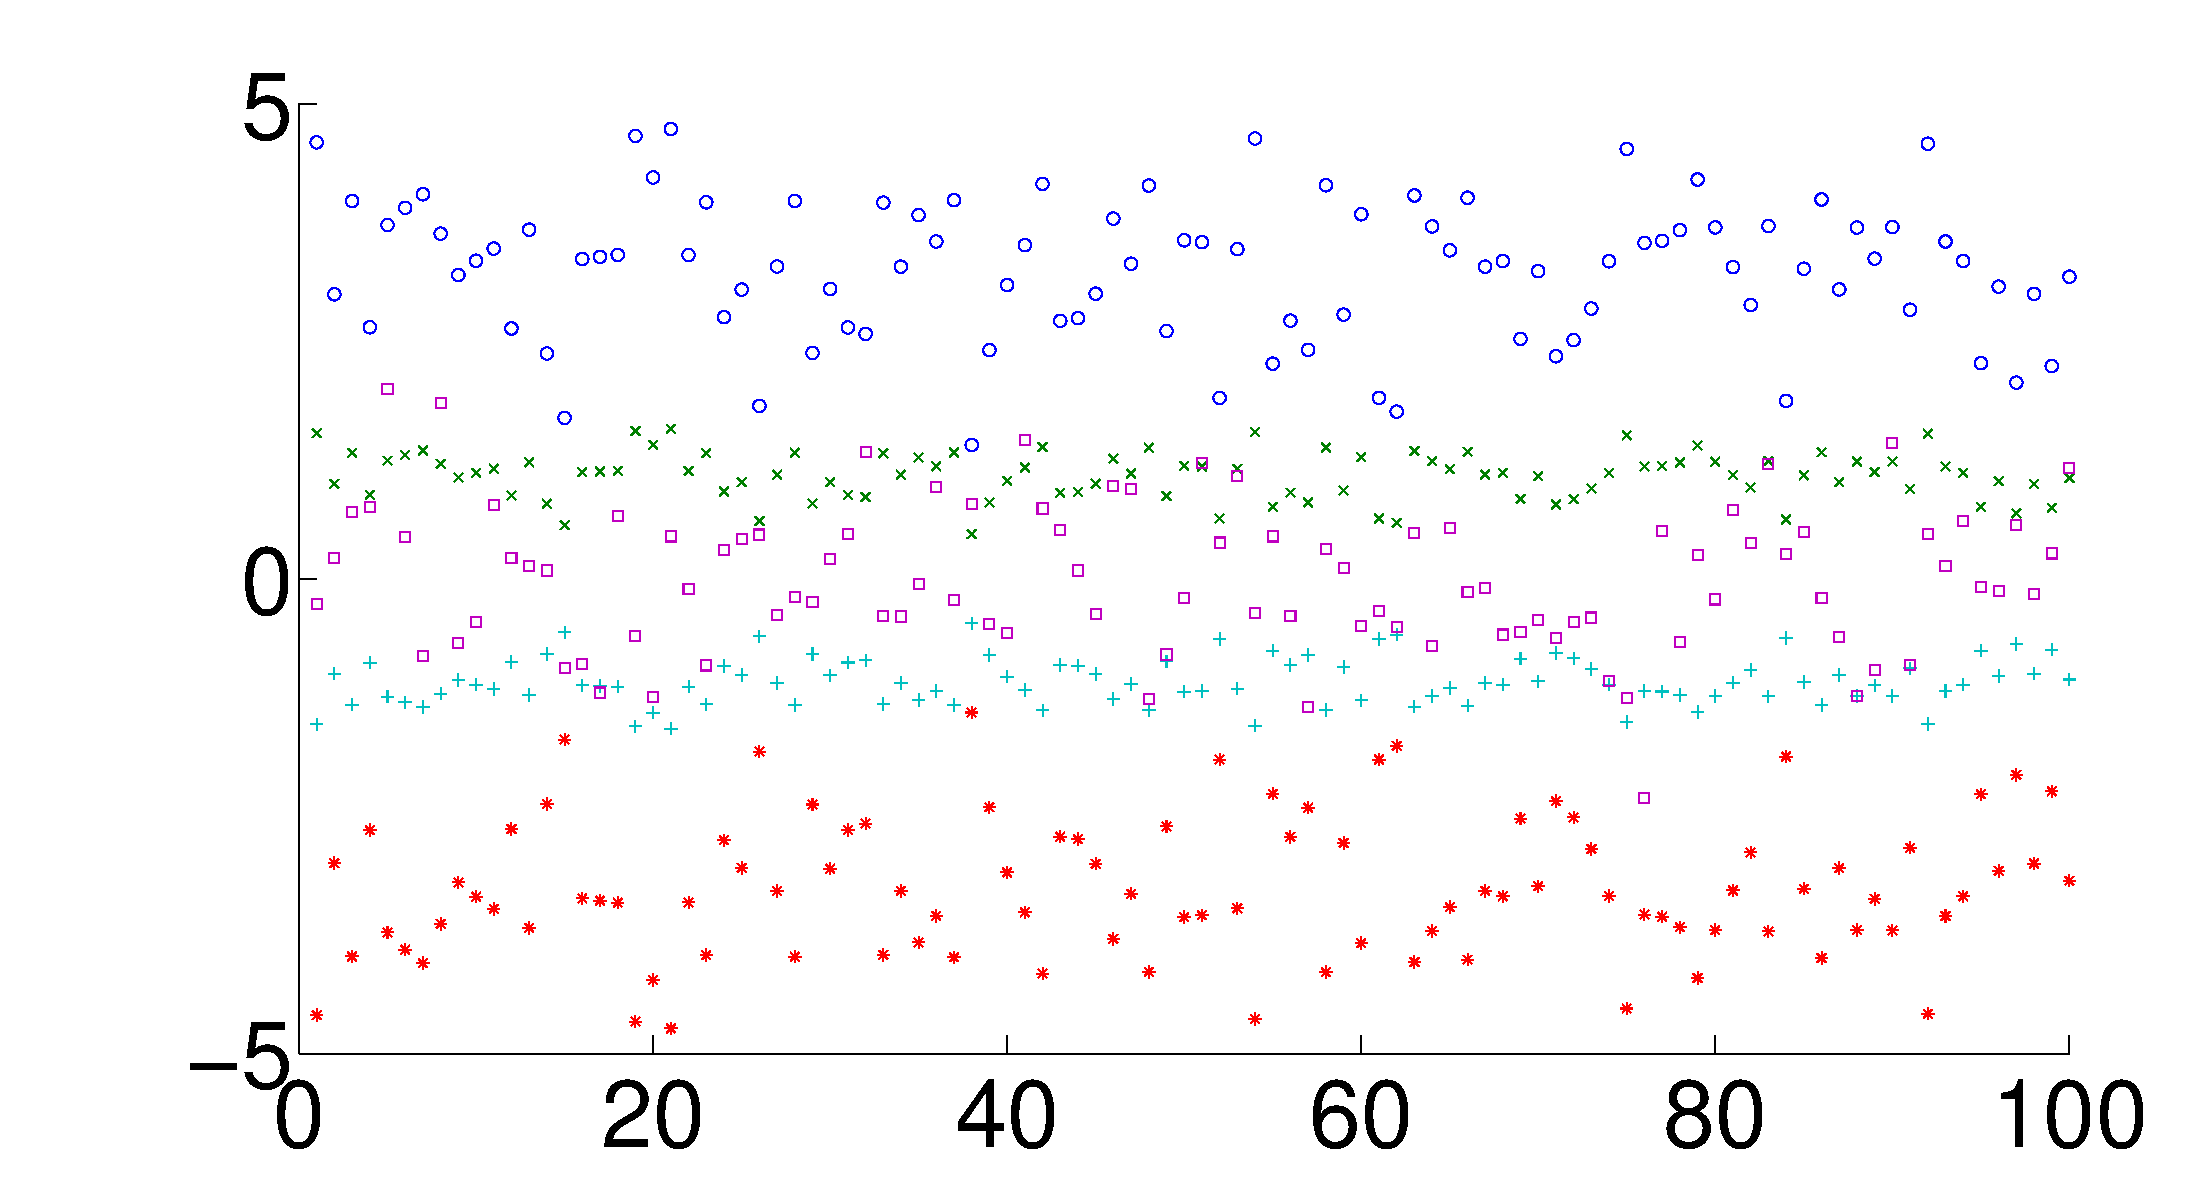
\includegraphics[scale=0.112]{fig/clusters.eps} &
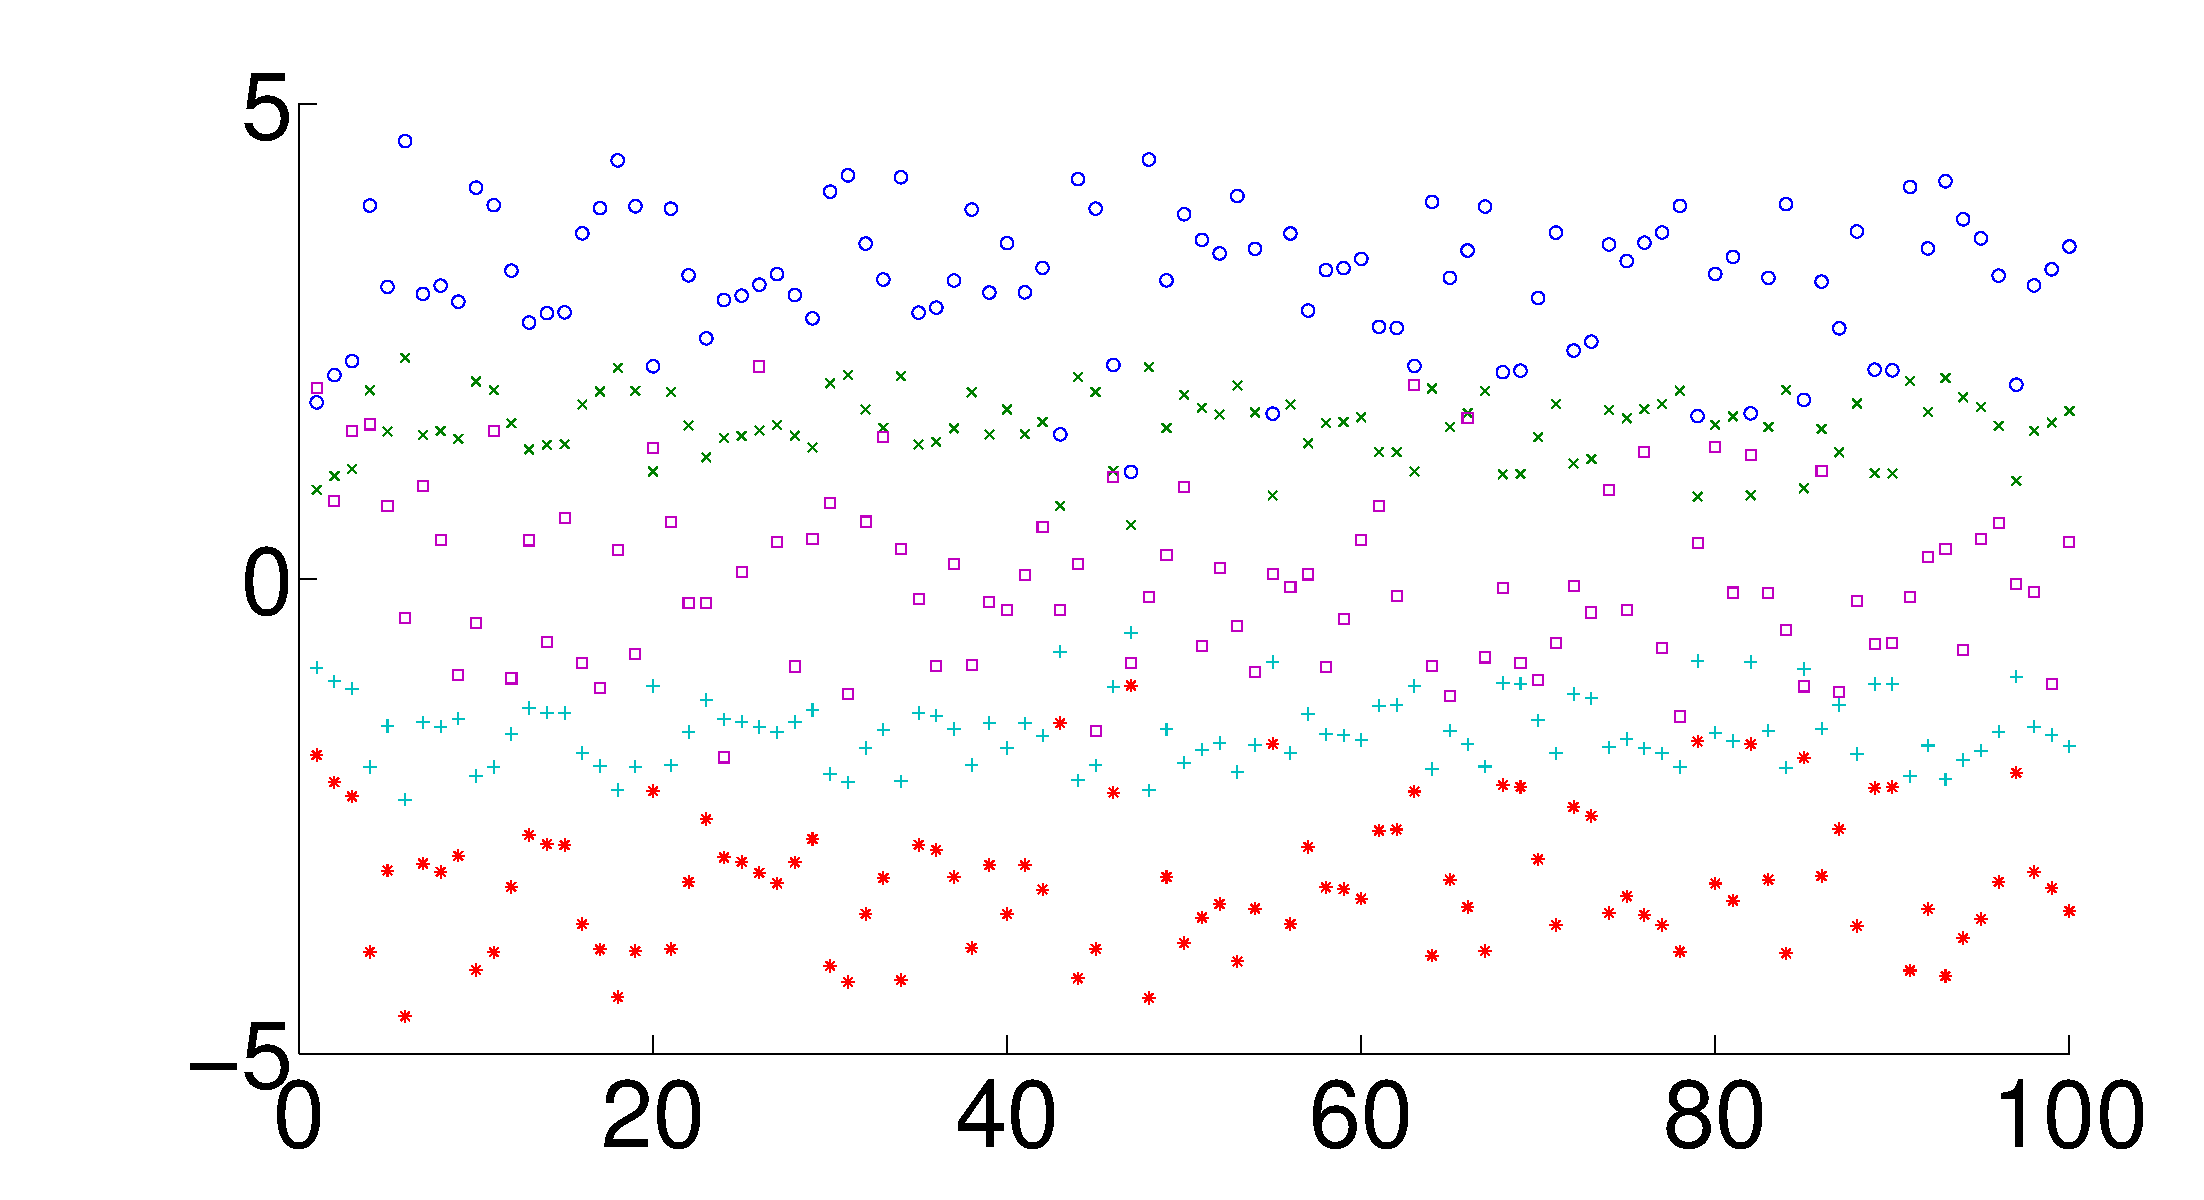
\includegraphics[scale=0.112]{fig/clusters4.eps} &
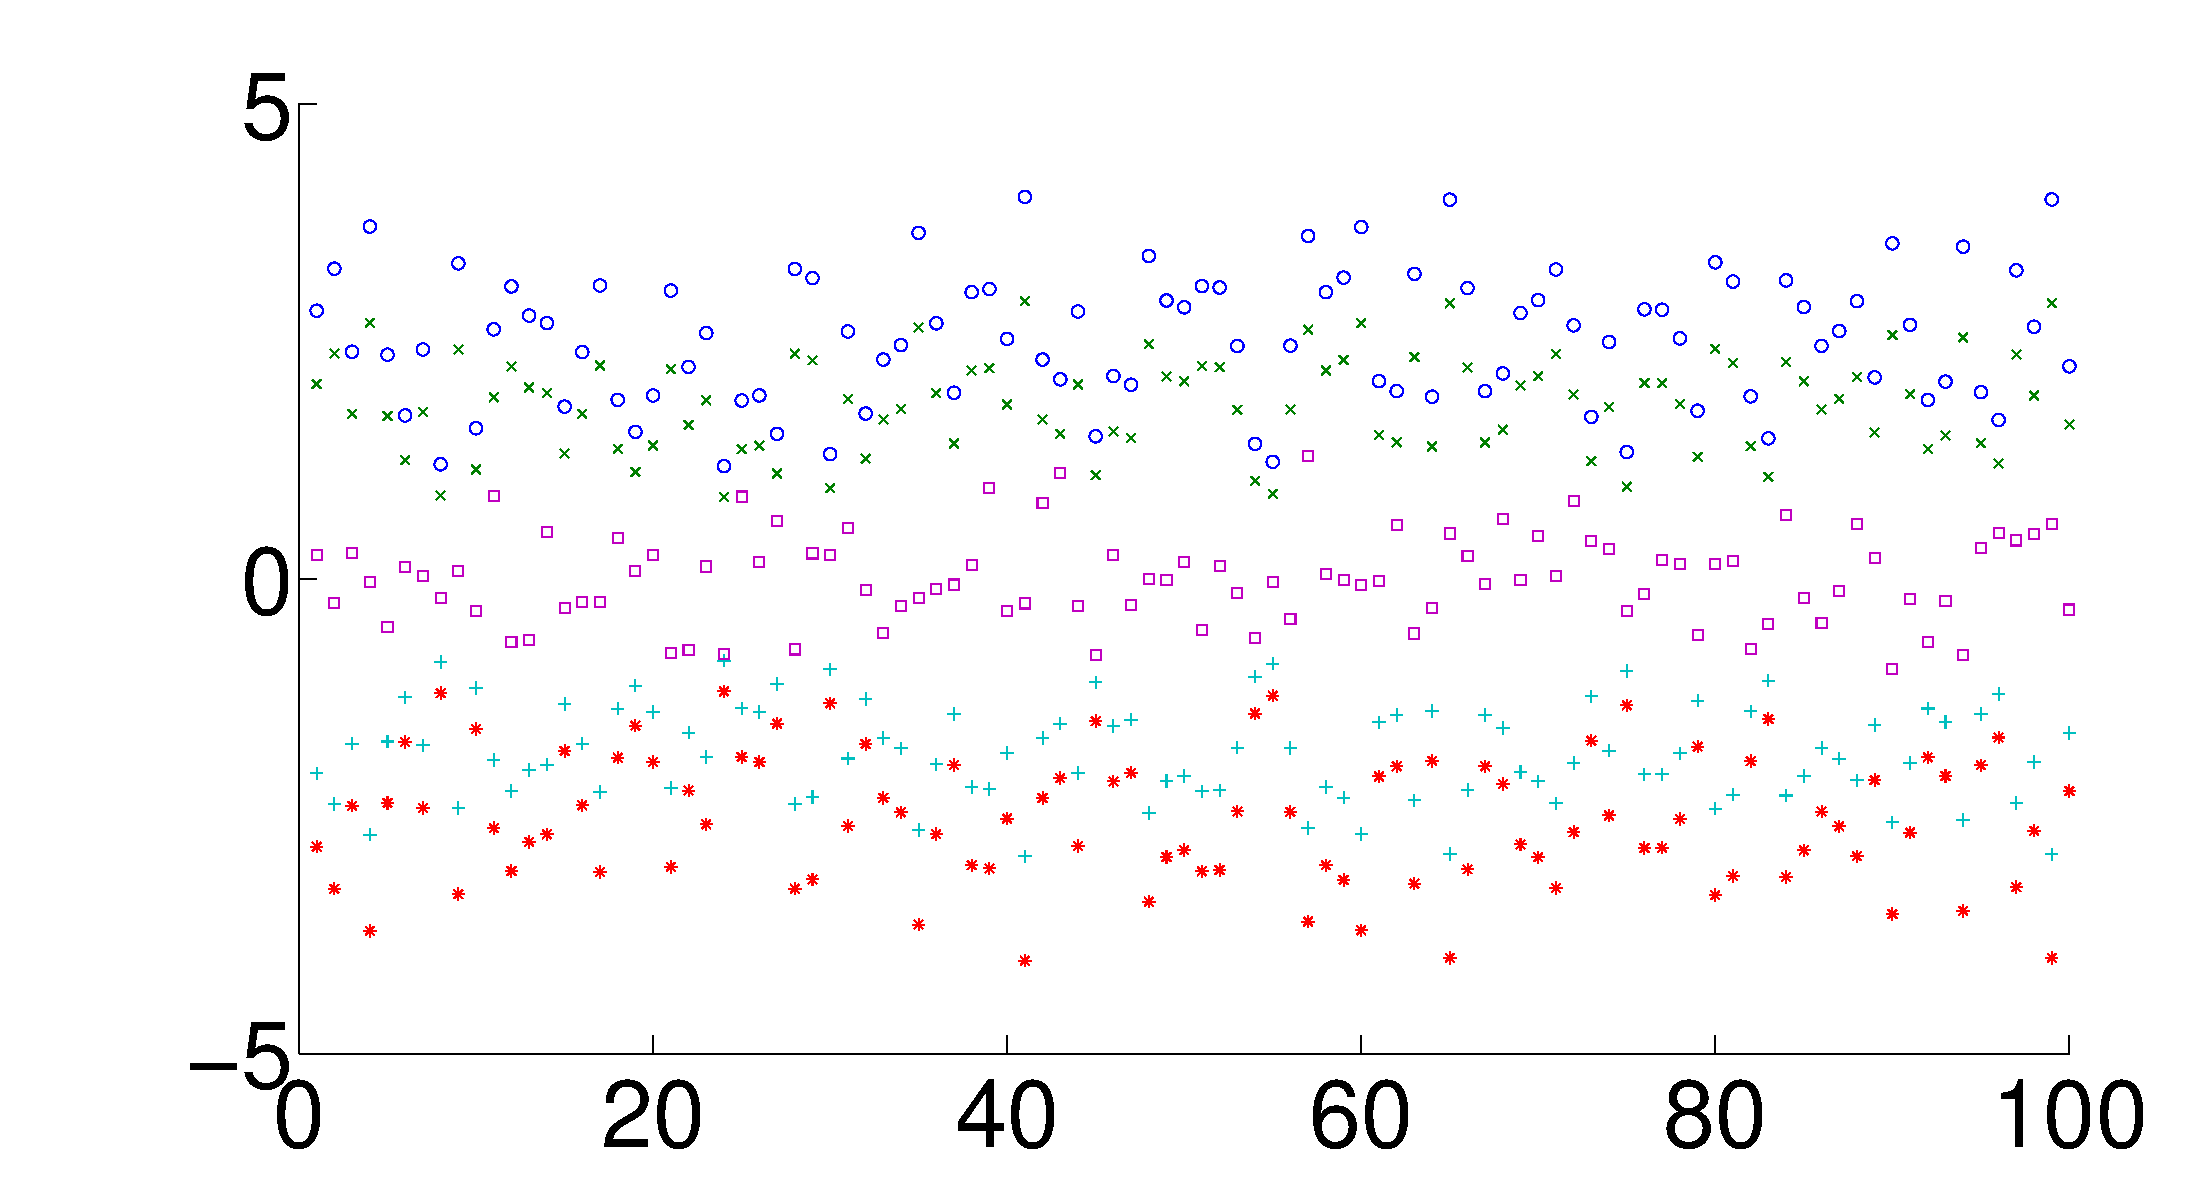
\includegraphics[scale=0.112]{fig/clusters3.eps} \\
$a_1$ --- range: [-4.74, 4.74] & $a_3$ --- range: [-4.61, 4.61] & $a_2$ --- range: [-4.02, 4.02] \\
$\mu$: 0, $\sigma$:2.26 &$\mu$: 0, $\sigma$:2.30 & $\mu$: 0, $\sigma$:2.18 \\
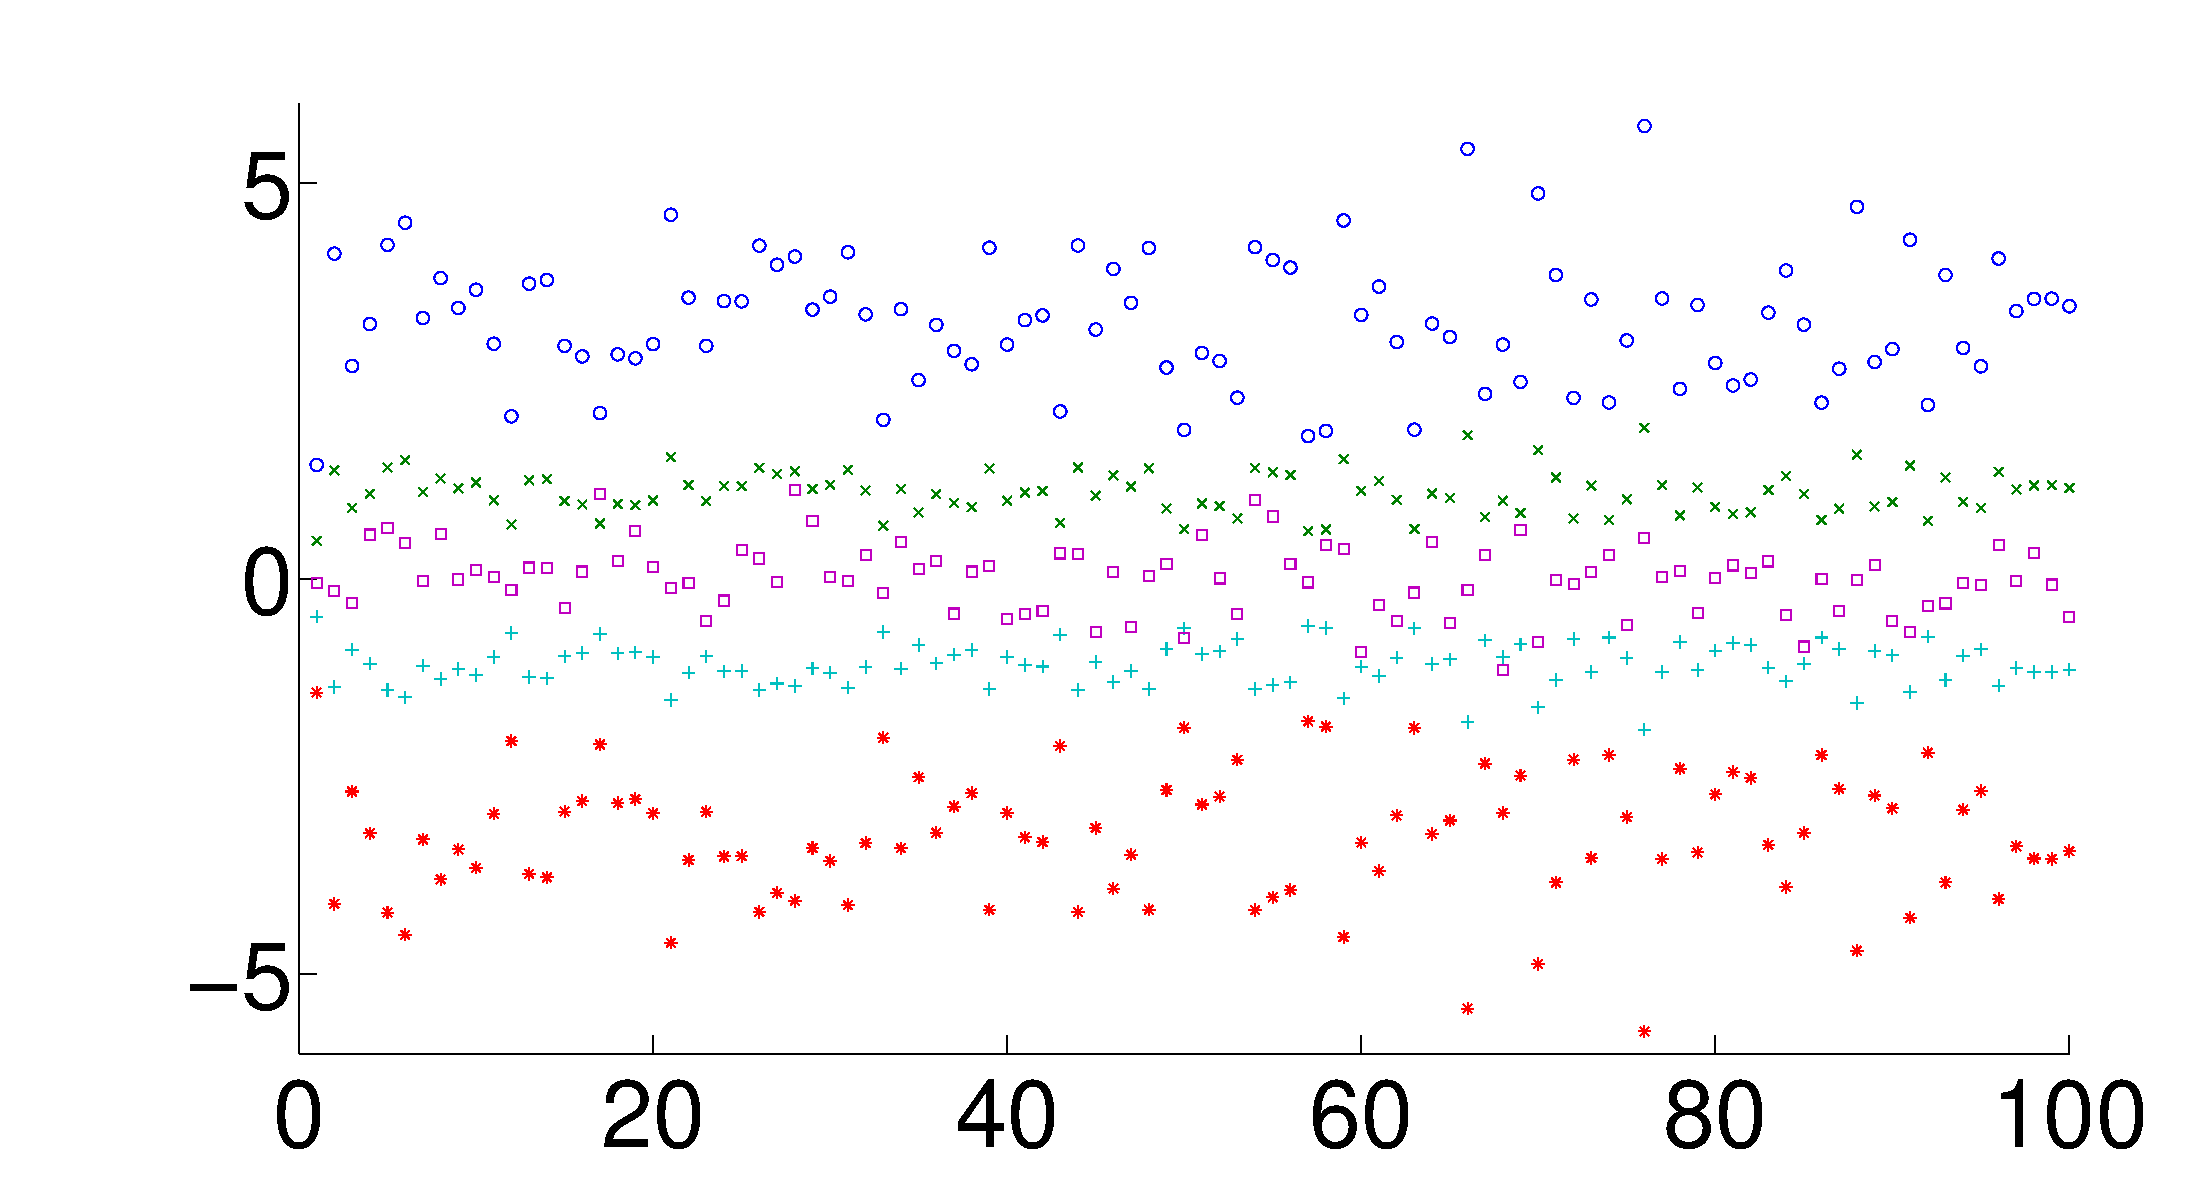
\includegraphics[scale=0.112]{fig/clusters21.eps} &
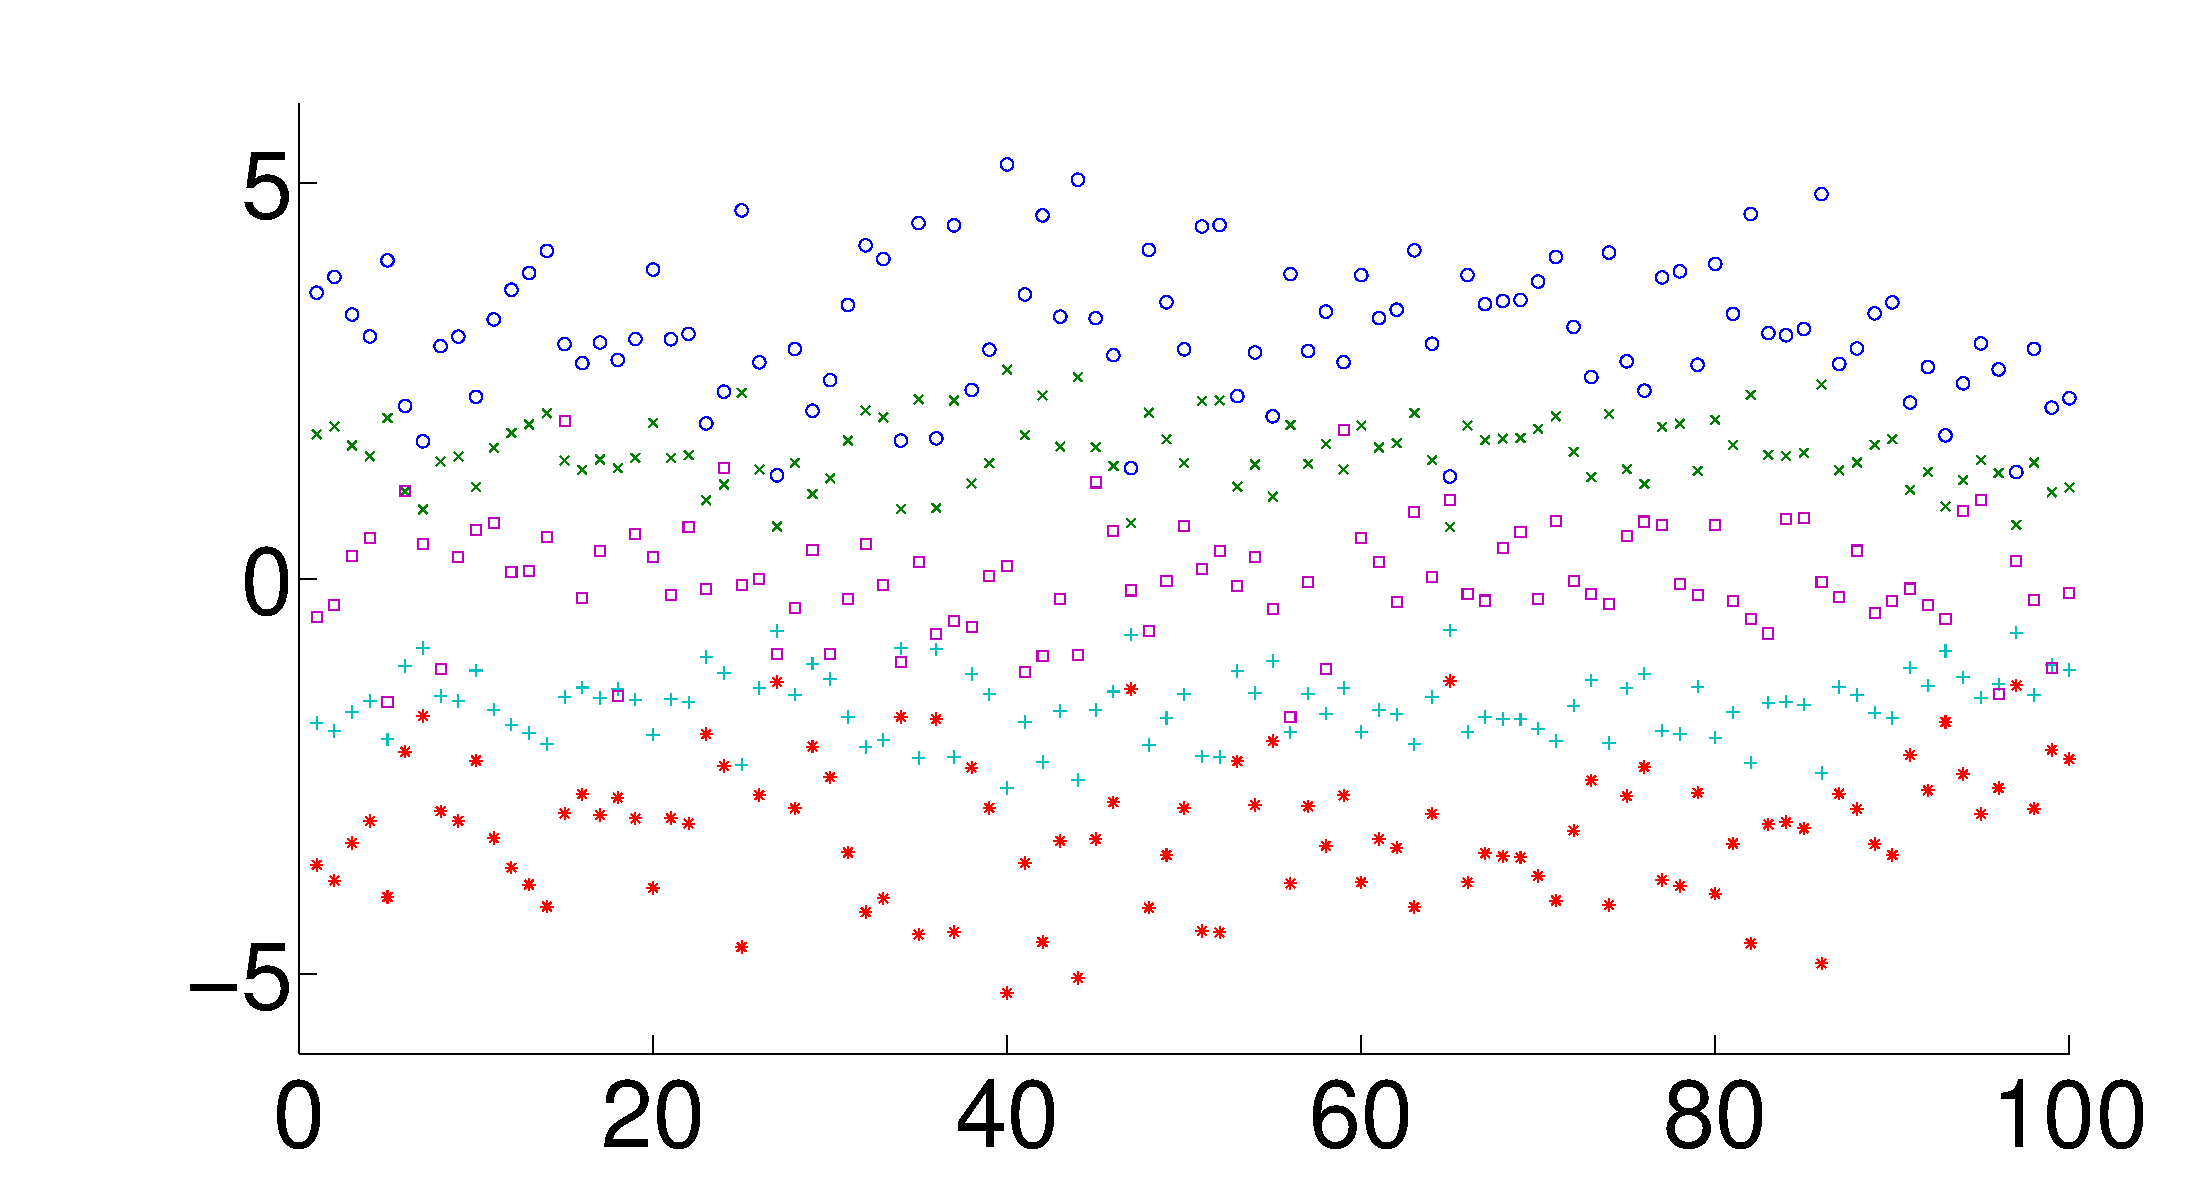
\includegraphics[scale=0.112]{fig/clusters23.eps} &
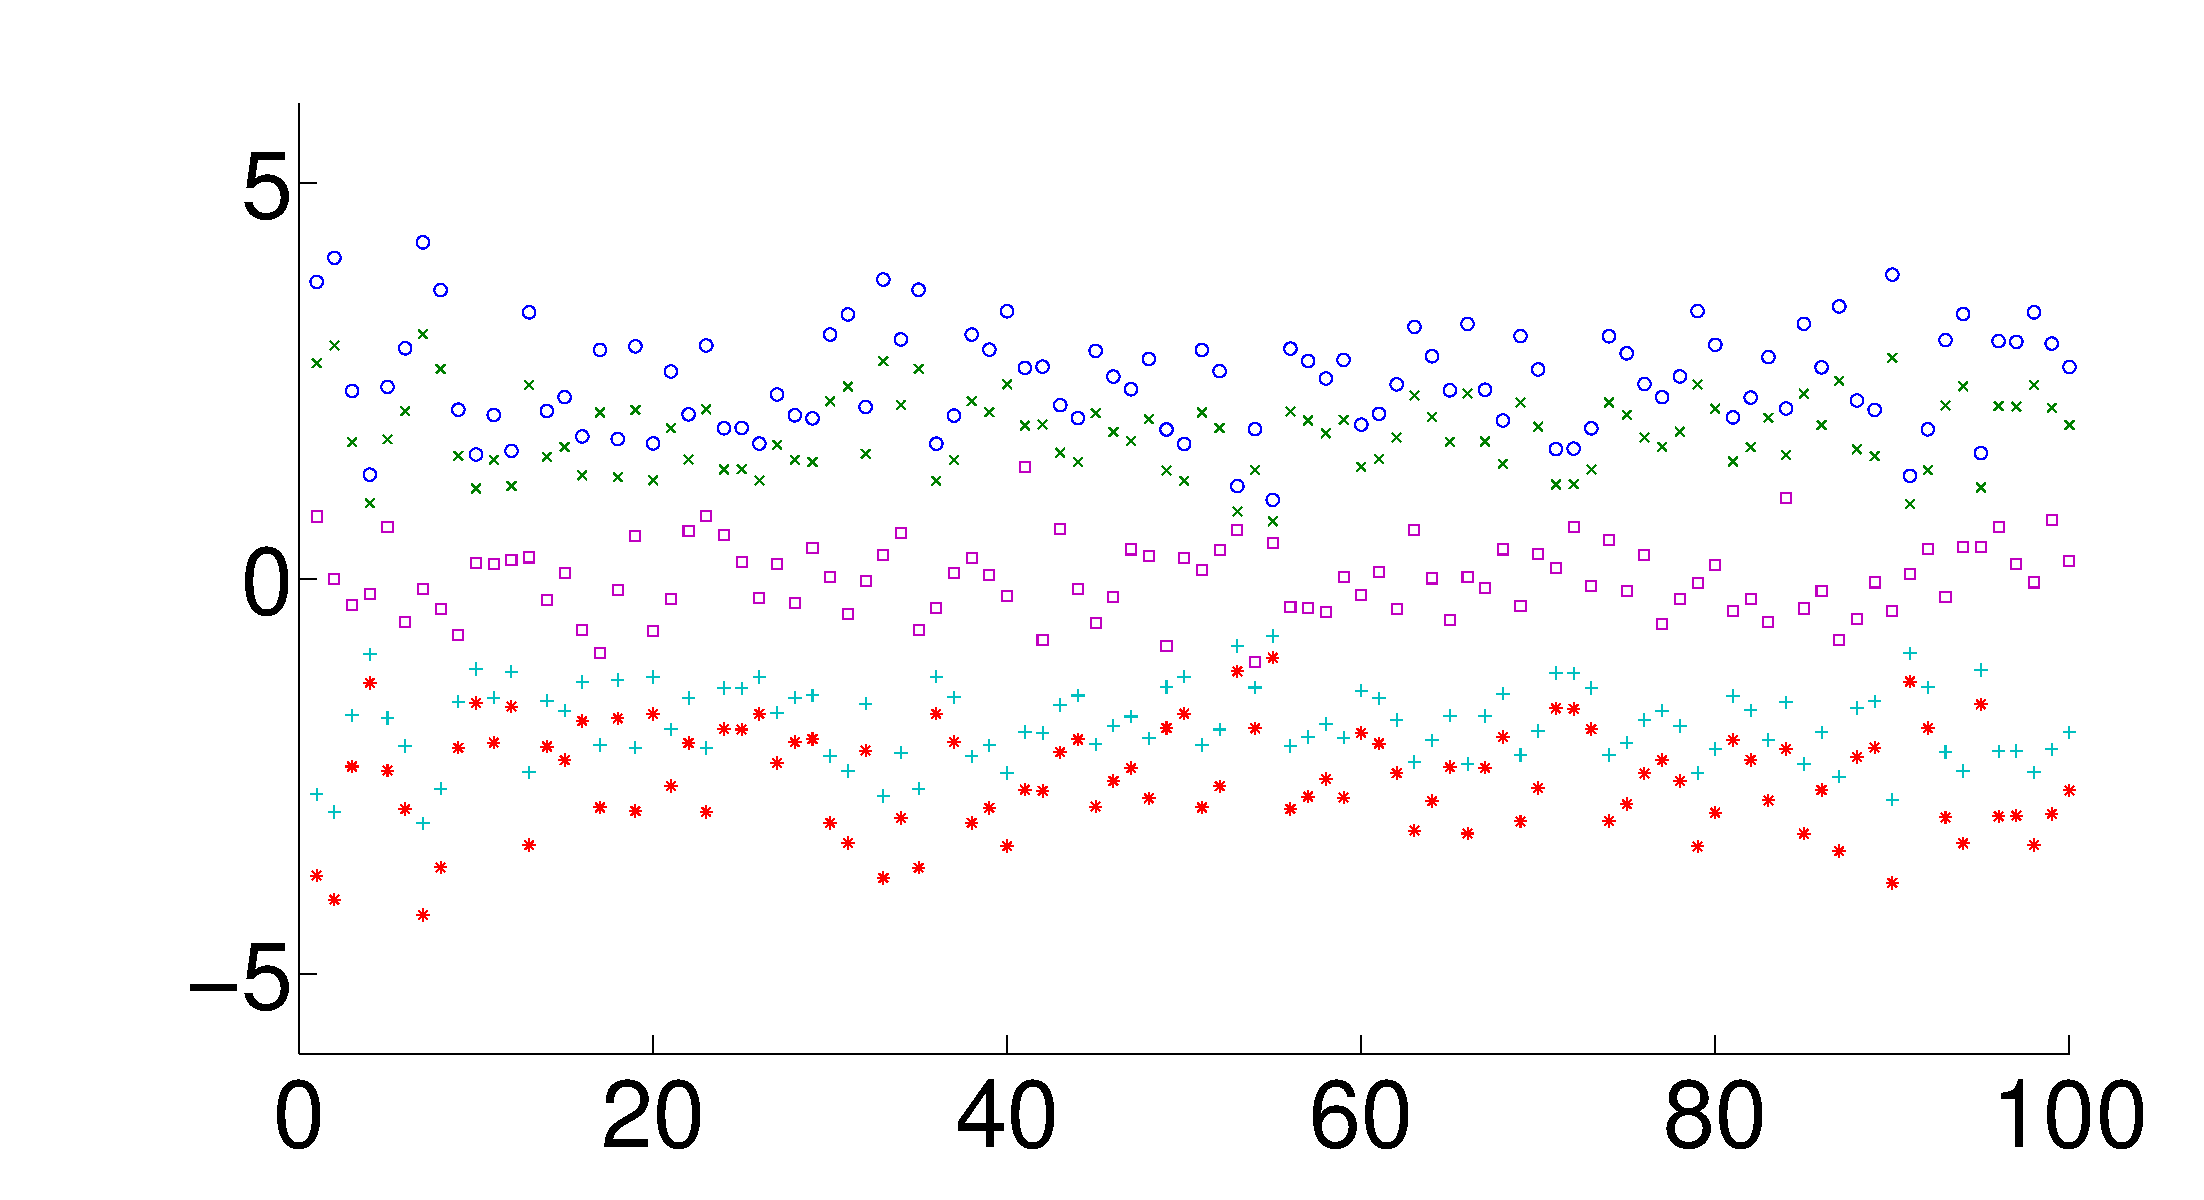
\includegraphics[scale=0.112]{fig/clusters22.eps} \\
$a_1'$ --- range: [-5.72, 5.72] & $a_3'$ --- range: [-5.24, 5.24] & $a_2'$ --- range: [-4.25, 4.25] \\
$\mu$: 0, $\sigma$:2.20 & $\mu$: 0, $\sigma$:2.35 & $\mu$: 0, $\sigma$:2.15 \\
\end{tabular}
\end{center}
\caption[Distribution of the synthetic dataset.]{\label{fig:syndata} Scatter plots of data instances from three sample attributes in one synthetic dataset (upper frame) and those of their corresponding attributes from another (lower frame) are illustrated to show their respective value distributions.}
\end{figure*}

\subsubsection{Results:}
Figure~\ref{fig:syn_pareto} illustrates the Pareto front obtained from matching two synthetic datasets, each having 20 attributes and 5 clusters. Most notably, the gold standard results for both attribute matching and cluster matching are obtained from the left-most point on the Pareto front. In other words, given the decision variables ($X$) corresponding to that point, we obtained 100\% correct matching results. We further observed that in our subsequent tests on other synthetic datasets with varied number of attributes and clusters, the derived Pareto fronts all contain the gold standard result, and the point corresponding to the gold standard can always be found towards the minimum end of $f_a$. Given this, we propose the following method to reduce the Pareto-optimal set to a single point corresponding to the most favored choice ($X^*$) in the decision space. The idea is to find the decision with the minimum weighted sum of objective values in the obtained Pareto-optimal set, i.e., $X^*=\stackbin[X]{}{\argmin}~\big[\alpha f_a(X)+\beta f_c(X)\big]$, where $\alpha$ and $\beta$ are weights. We first conducted preliminary experiments to determine the best values for $\alpha$ and $\beta$ (0.8 and 0.2 respectively) and used them in all subsequent experiments. This method works markedly well on the synthetic datasets. For all the tests described in Table~\ref{tbl:scale}, 100\% correct results for both attribute and cluster matchings are obtained (hence we omit the precision in the table).

Notice that it is common in multi-objective optimization problems that a non-dominated set may be too large for decision makers to reasonably consider. However, it is shown in Figure~\ref{fig:syn_pareto} (as well as results from other experiments described in the following) that this is not the case using our method on datasets of representative sizes in attribute and clustering matching problems. The number of resulting Pareto optimal solutions is small enough to be presented to decision makers without the need of any means of reducing or organizing the non-dominated set. The reason why we use a straightforward weighted sum method to compute the most significant solution from Pareto front is because it empirically works well on our test cases, this step is not obliged because a decision maker can go over solutions in Pareto front and decide which one is the best.

\begin{figure}[tb]
\begin{center}
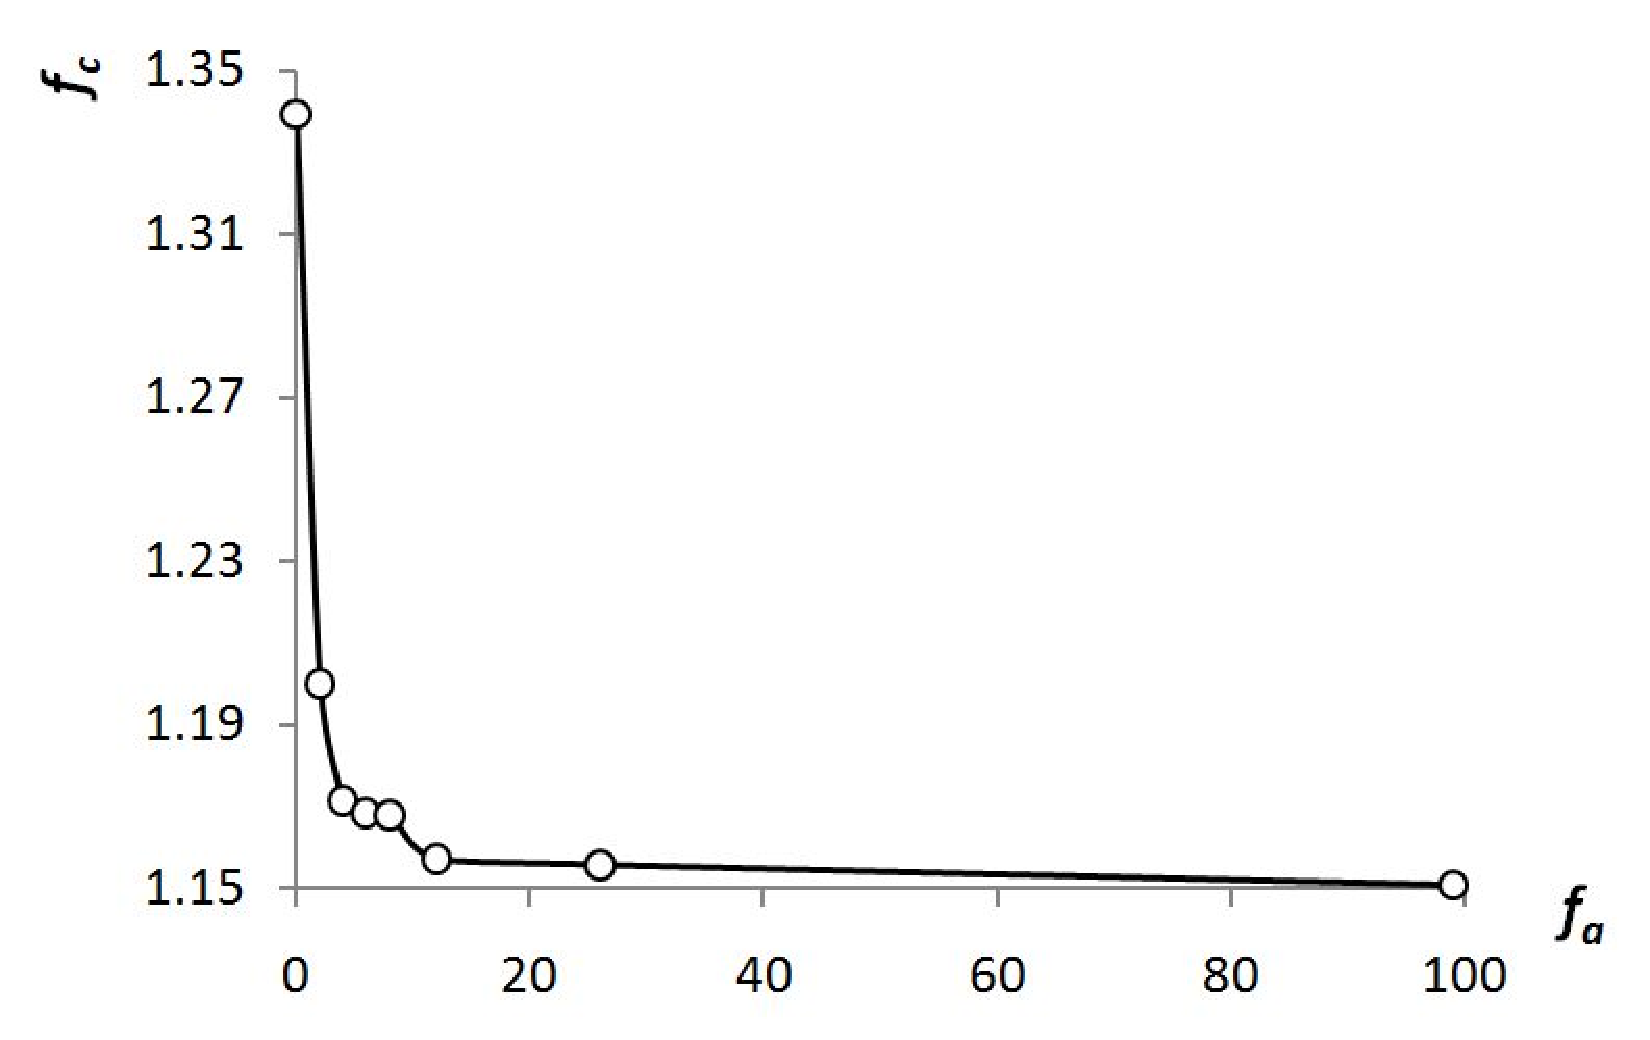
\includegraphics[width=0.4\textwidth]{fig/syn_pareto.eps}
\end{center}
\caption[An example Pareto front result from the synthetic dataset]{\label{fig:syn_pareto} An example Pareto front obtained from matching two synthetic datasets with 20 attributes and 5 clusters.}
\end{figure}

\subsubsection{Running Time:}
We systematically altered the number of attributes and clusters present in the data and conducted a series of tests to show the scalability of the proposed method. The running time under different configurations is reported in Table~\ref{tbl:scale}. The time is calculated by averaging over 5 runs of each test (on a 2.53GHz dual-core CPU with 4 gigabytes memory), each run having 1000 iterations in the simulated annealing process. The main computationally expensive part of the annealing process is the generation of new candidate solution phase (function $G$) in which an assignment problem is solved using the Hungarian method. The complexity of the Hungarian method is cubic and is already the most efficient algorithm for solving the assignment problem (e.g., a brute force algorithm has a factorial complexity). Fortunately, rarely is the case that the number of attributes or clusters is large in real-world scenarios where the proposed technique is needed. For reasonable configurations in most practical applications, the computation time is within a tractable range as shown in table~\ref{tbl:scale}.
\begin{table}[tbh]
\begin{center}
\begin{tabular}{r|r|r}
\hline
\# attributes & \# clusters & time (sec)\\
\hline
5   &   20  &   0.28\\
20  &   20  &   1.81\\
20  &   40  &   7.04\\
20  &   60  &   17.80\\
40  &   20  &   4.66\\
40  &   40  &   11.74\\
40  &   60  &   25.93\\
60  &   20  &   10.95\\
60  &   40  &   20.70\\
60  &   60  &   37.35\\
100 &   100 &   172.23\\
\hline
\end{tabular}
\end{center}
\caption[Running time on the synthetic dataset]{\label{tbl:scale} Running time of the annealing process on synthetic datasets with varied configurations of attribute and cluster sizes. The time is obtained by averaging over results of 5 runs of each test.}
\end{table}

\subsection{Neuroscience Dataset}
\subsubsection{Data Acquisition:}
%The difficulty is especially pronounced in many scientific domains where there have been an increasing interest in nationwide and worldwide inter-institute collaboration. An example of such collaborative project is research in experimental event-related brain potential (ERP) analysis carried out at the NEMO (Neural Electromagnetic Ontologies) consortium laboratories. The heterogeneity among participating groups hinders meaningful meta-analysis despite the large number of studies in the field.

To address the problems of attribute and cluster matching in a real-world neuroscience application, we used a set of realistic simulated ERP (event-related potentials) datasets, which were designed to support evaluation of ERP analysis methods~\cite{FrishkoffEtal07}. The datasets were specifically designed to simulate heterogeneous data from different groups of subjects under different conditions (via distinct simulated brain activities), as well as distinct measurement methods (spatial and temporal metrics) and distinct patterns (reflecting two different pattern decomposition techniques). Real ERP data arise from superposition of latent scalp-surface electrophysiological patterns, each reflecting the activity of a distinct cortical network that cannot be reconstructed from the scalp-measured data with any certainty. Thus, real ERP data are not appropriate for evaluation of ERP pattern mapping. By contrast, simulated ERP data are derived from known source patterns and therefore provide the necessary gold standard for evaluation of our proposed methods.

The raw data for this study consist of 80 simulated event-related potentials (ERPs), in which each ERP comprises simulated measurement data for a particular subject ($n$ = 40). The 40 simulated subjects are randomly divided into two 20-subject groups, SG1 and SG2, each containing 40 ERPs (20 subjects in 2 experimental conditions). Each ERP consists of a superposition of 5 latent varying spatiotemporal patterns. These patterns were extracted from the two datasets, SG1 and SG2, using two techniques: temporal Principal Components Analysis (tPCA) and spatial Independent Components Analysis (sICA), two data decomposition techniques widely used in ERP research~\cite{Dien2010}. To quantify the spatiotemporal characteristics of the extracted patterns, two alternative metric sets, m1 and m2, were applied to the two tPCA and the two sICA derived datasets. For a complete explanation of these alternative metrics, please see Appendix in~\cite{FrishkoffEtal07}.

In summary, the simulated ERP data generation process yielded eight test datasets in total, reflecting a 2 (attribute sets) $\times$ 2 (subject groups) $\times$ 2 (decomposition methods) factorial design. Therefore, for each attribute set there are 4 datasets generated from different combinations of subject groups and decomposition methods, resulting $4 \times 4 = 16$ cases for the studies of attribute matching and cluster matching. The reason to include such variabilities was to test the robustness of our matching method to different sources of heterogeneities across the different datasets. Within all test datasets, 5 major ERP spatiotemporal patterns are present. They are P100, N100, N3, MFN, and P300. These patterns can be identified in the datasets by clustering analysis. Pretending that the latent patterns underlying discovered clusters are unknown, we hope to match clusters across datasets to recover the fact that the same patterns are present in all datasets.

\subsubsection{Results:}
%Figure~\ref{fig:nemo_exp} illustrates the Pareto fronts derived by the proposed method on each of the 16 test cases.
We applied the weighted sum method as the post-processing step after obtaining the Pareto-optimal solutions to determine the most favored choice using the parameters ($\alpha$ and $\beta$) discovered in the preliminary experiments on synthetic datasets (cf. Section~\ref{sec:syn_exp}). The accuracy of attribute matching and cluster matching along with the number of points in the Pareto front are listed in Table~\ref{tbl:nemo_perf} (all these results are obtained by taking average from 5 runs for each test case).

%\begin{figure*}[tb]
%\begin{center}
%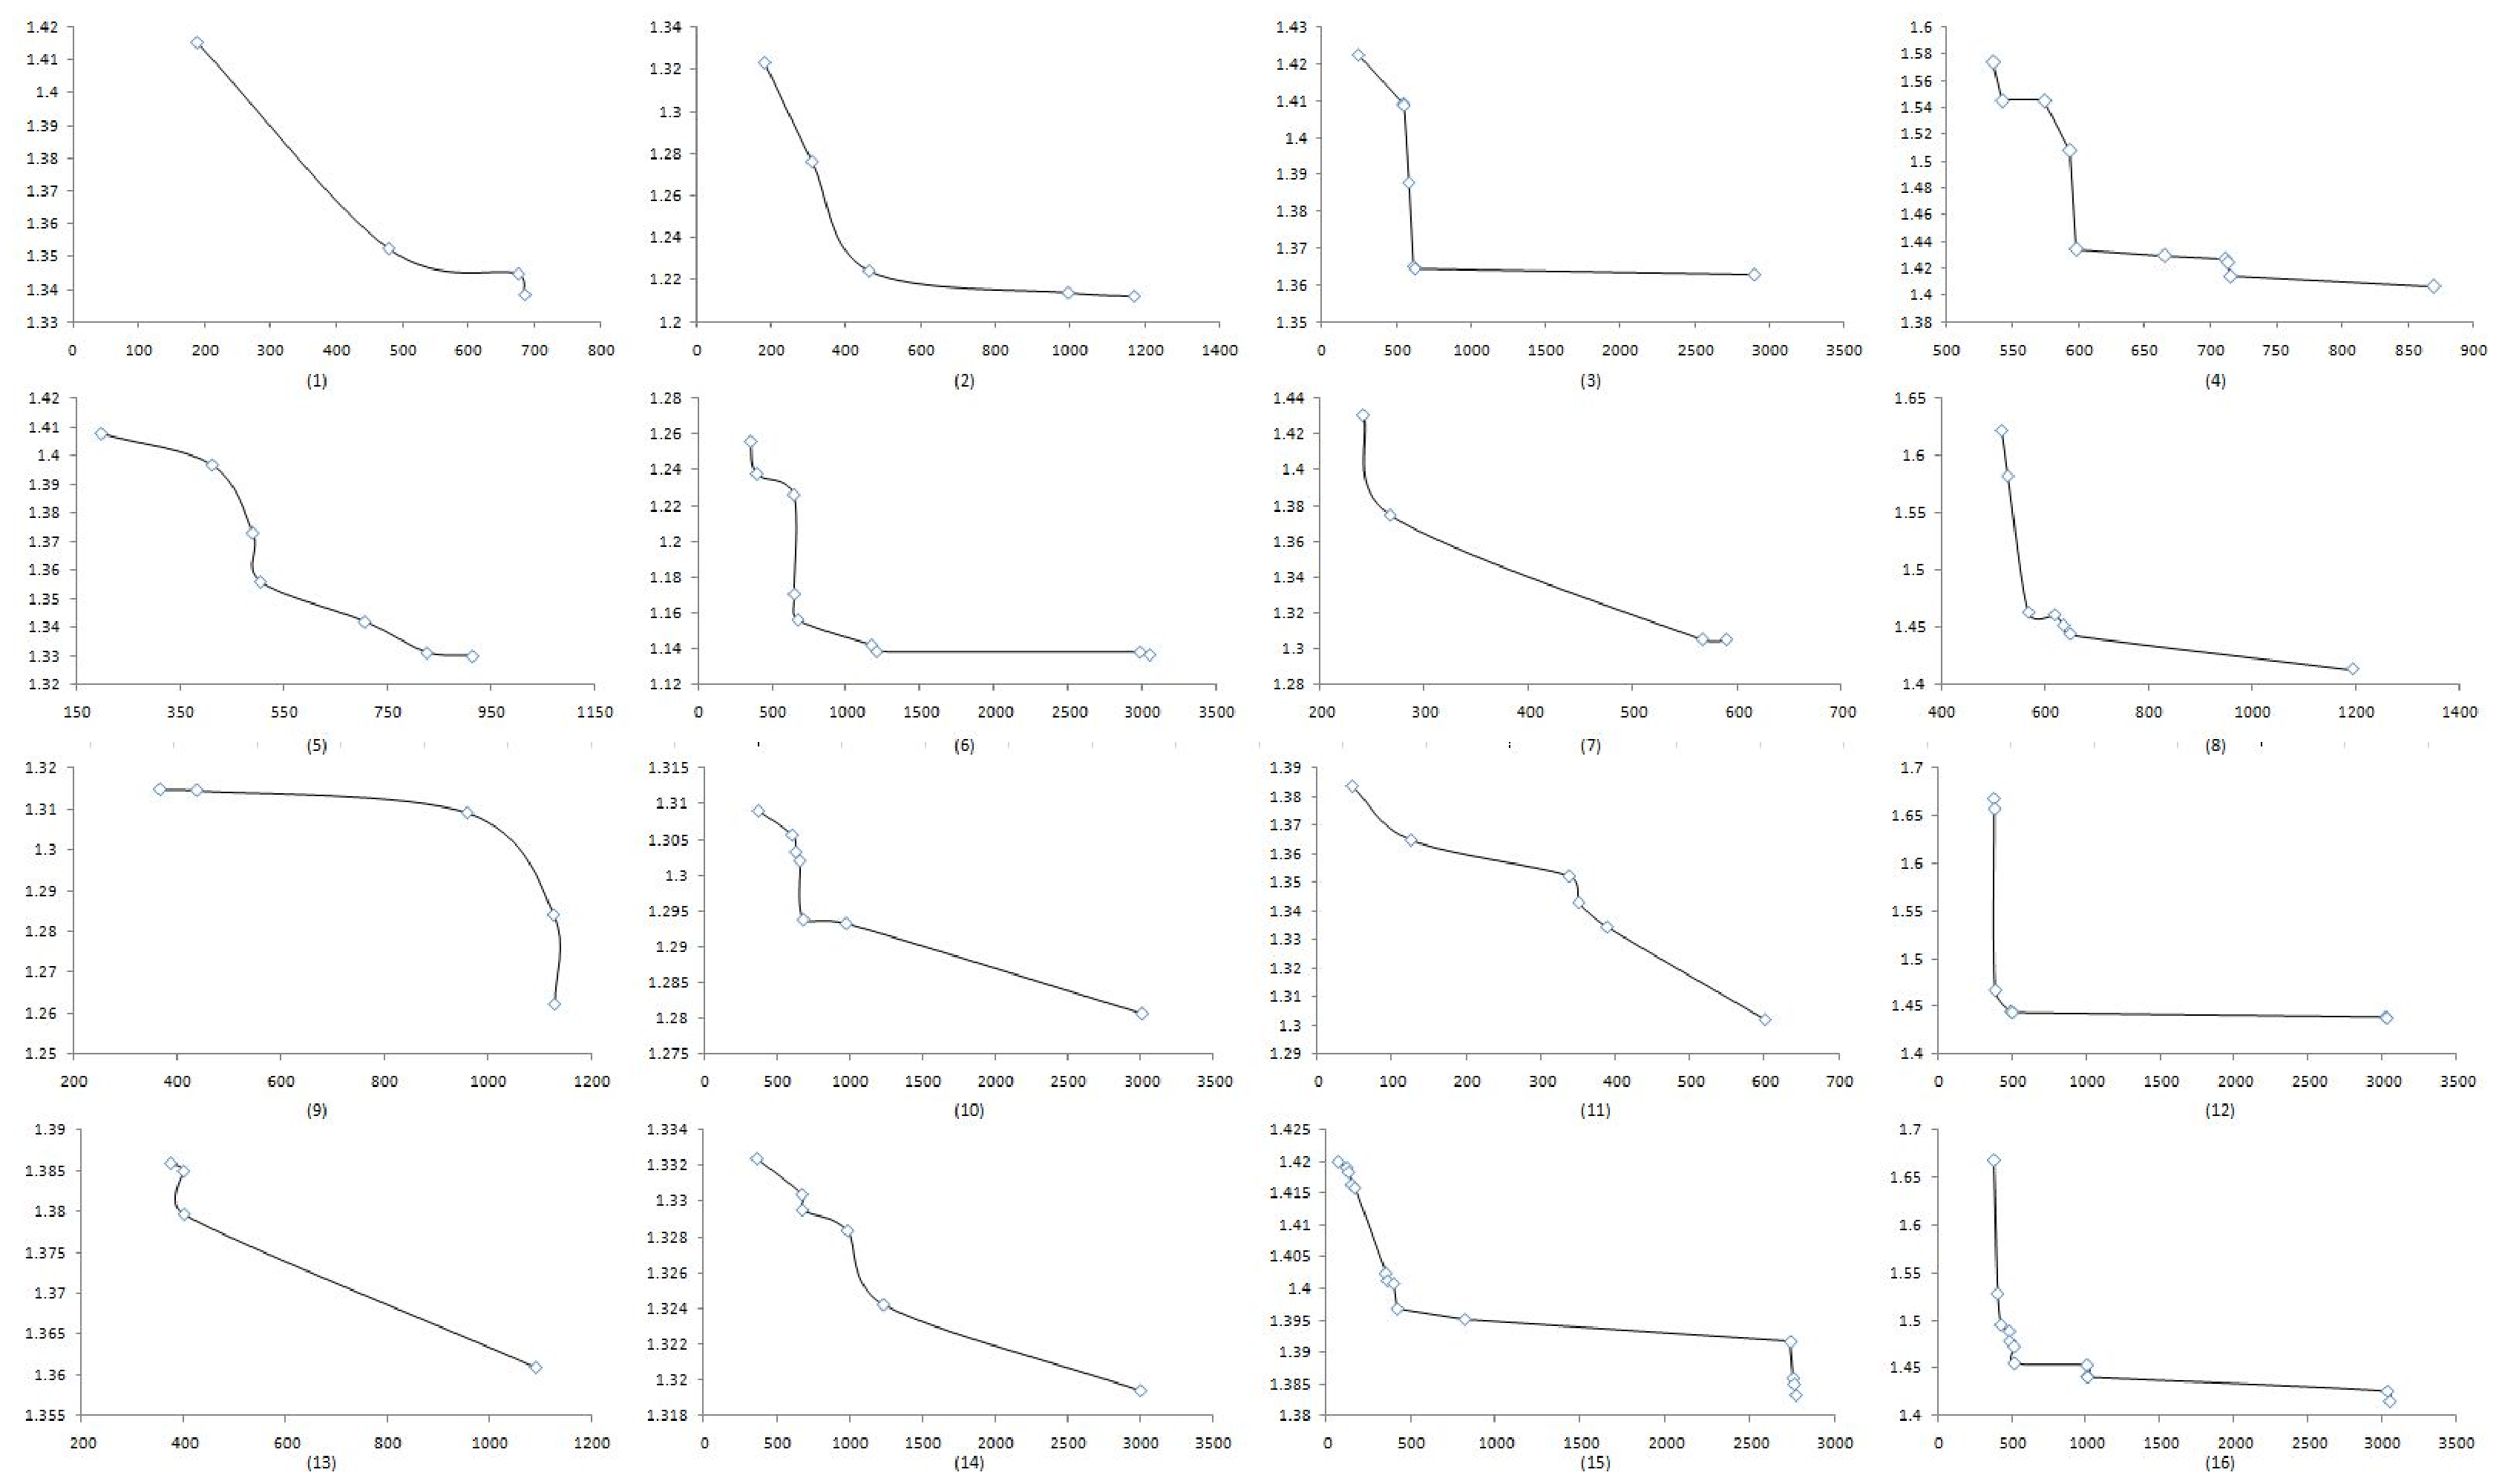
\includegraphics[width=1.\textwidth]{nemo_exp2.eps}
%\end{center}
%\caption{\label{fig:nemo_exp} Pareto fronts obtained from the 16 test cases of the neuroscience dataset.}
%\end{figure*}

It can be observed from the results in Table~\ref{tbl:nemo_perf} that more different factors involved in the acquisition of the two datasets for matching can negatively affect the matching performance. For example, in test case 1, the two datasets are drawn from the same subject group (SG1) and preprocessed using the same decomposition method (sICA); whereas in test case 4, the subject groups and decomposition methods are all different, resulting in greater variability and hence the performance is less satisfactory.

It is worth noting that our method greatly outperforms a baseline method called WS (see Figure~\ref{fig:perf_comp}) that determines attribute matching based on data distribution at the whole attribute level, which is typical in previous systems such as SemInt~\cite{Li00semint:a}. In this figure we also demonstrate the accuracy of the segmented statistics characterization with expert-labeled patterns, meaning that the data is partitioned and aligned in the most accurate way, which marks the best achievable attribute matching performance. But it is not feasible because manually recognizing patterns (partitioning data) and aligning them across datasets requires a priori knowledge of attributes in the datasets which is exactly what the problem of attribute matching tries to discover (the circular causality problem). On the other hand, our method does not require human involvement (except the specification of the number of clusters (patterns) present in the data in order to run the clustering analysis) in determining both the attribute matching and cluster matching and is able to achieve close-to-optimal results.

\begin{figure*}[tb]
\begin{center}
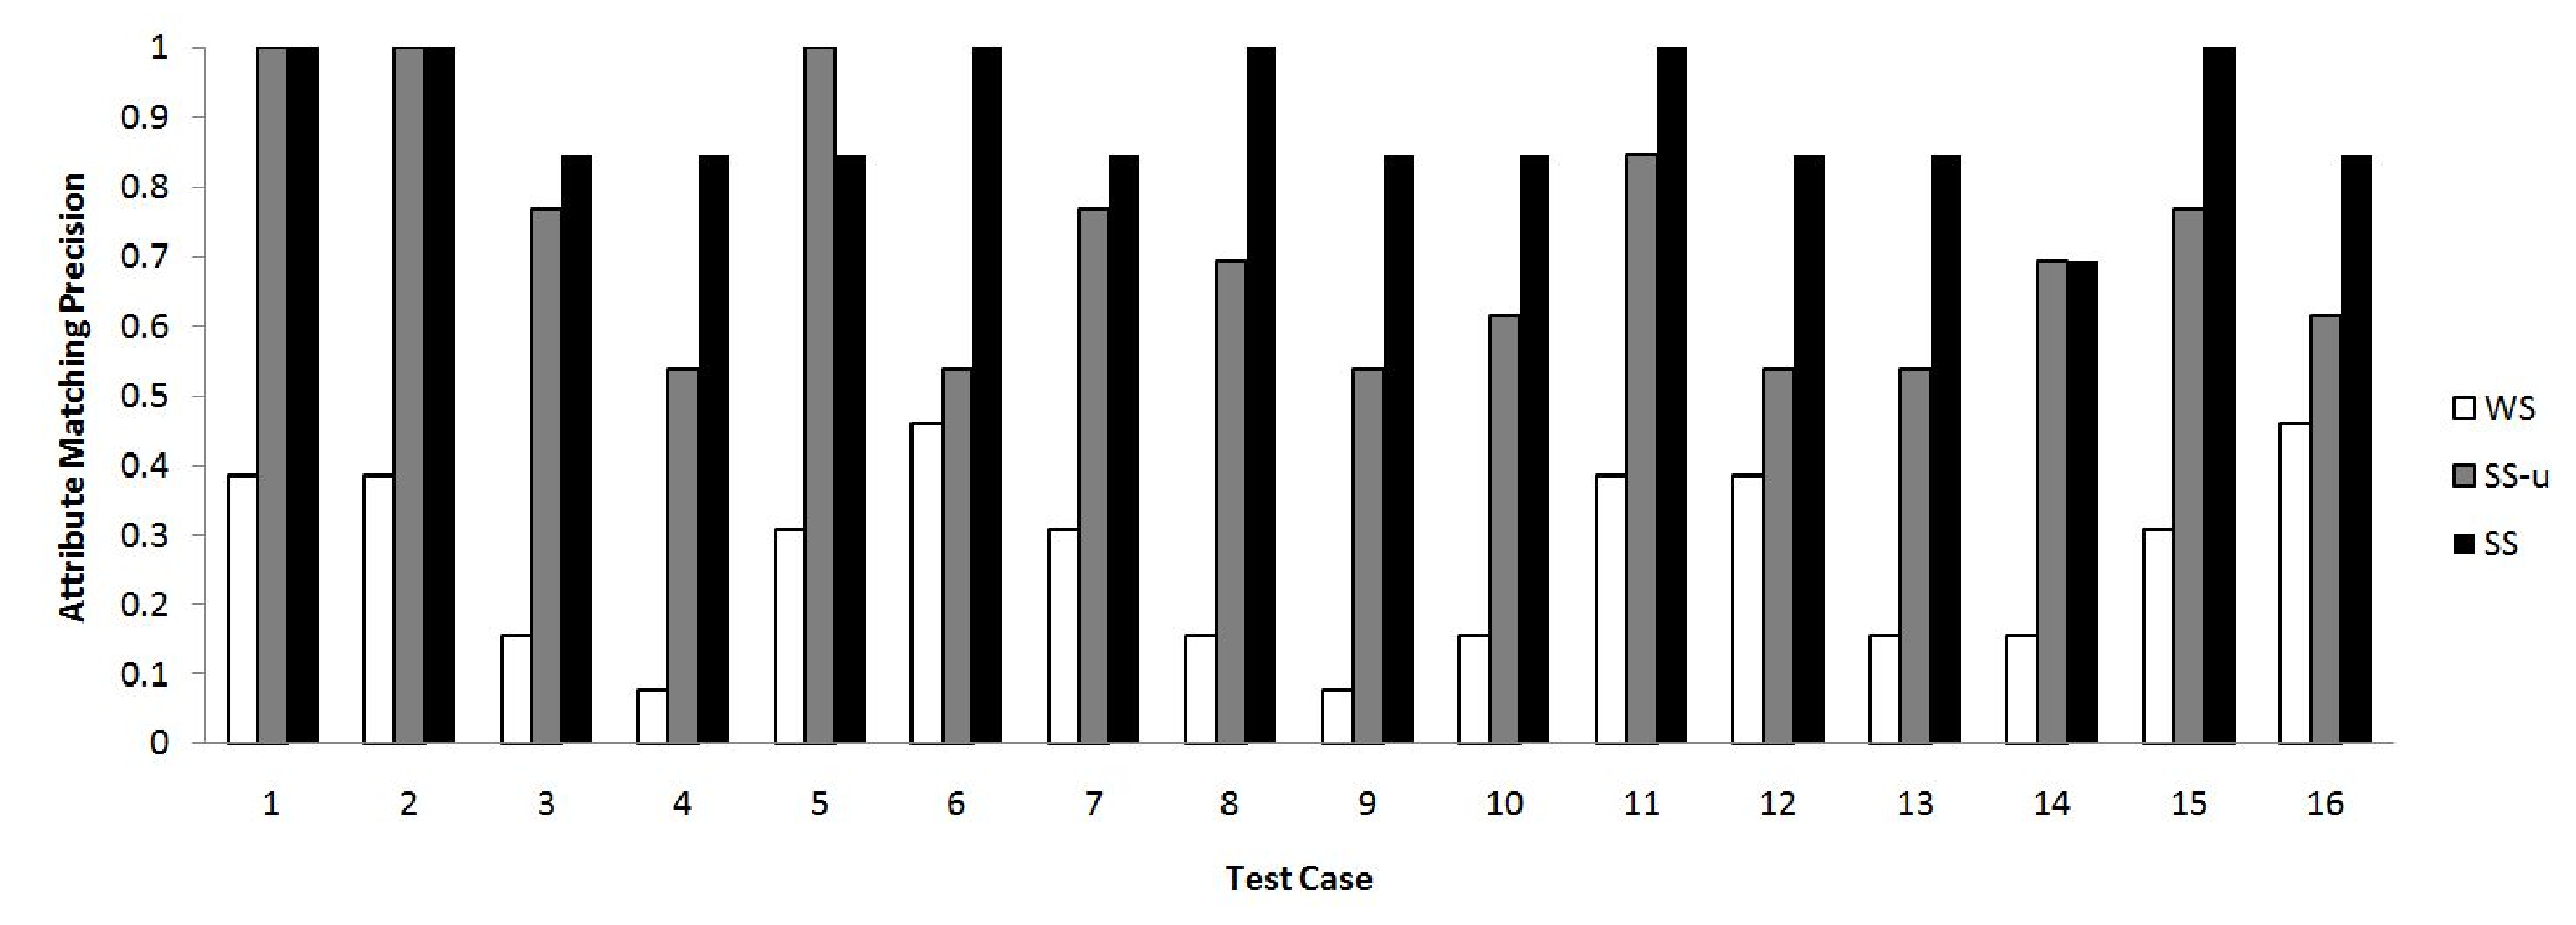
\includegraphics[width=1.\textwidth]{fig/perf_comp.eps}
\end{center}
\caption[A comparison between methods on the neuroscience dataset]{\label{fig:perf_comp} A comparison of the attribute matching accuracy of three methods on the 16 test cases of the neuroscience dataset. The three methods being compared are matching based on whole-attribute statistics (WS), segmented attribute statistics without knowing a priori cluster matching (SS-u), and segmented attribute statistics with expert-aligned clusterings (SS).}
\end{figure*}


\begin{table*}[tbh]
\begin{center}
\begin{tabular}{l|l|l|l|l|l}
\hline
Test case & Source params & Target params & $~~~P_a~~~$ & $~~~P_c~~~$ & $|\Sigma|$\\
\hline
1		&	$\langle$	SG1, sICA, m1	$\rangle$	&	$\langle$	SG1, sICA, m2	$\rangle$	&		13/13	&	5/5	&	5	 \\
2		&	$\langle$	SG1, sICA, m1	$\rangle$	&	$\langle$	SG2, sICA, m2	$\rangle$	&		13/13	&	5/5	&	6	 \\
3		&	$\langle$	SG1, sICA, m1	$\rangle$	&	$\langle$	SG1, tPCA, m2	$\rangle$	&		10/13	&	5/5	&	6	 \\
4		&	$\langle$	SG1, sICA, m1	$\rangle$	&	$\langle$	SG2, tPCA, m2	$\rangle$	&		7/13	&	3/5	&	8	 \\
5		&	$\langle$	SG2, sICA, m1	$\rangle$	&	$\langle$	SG1, sICA, m2	$\rangle$	&		11/13	&	3/5	&	7	 \\
6		&	$\langle$	SG2, sICA, m1	$\rangle$	&	$\langle$	SG2, sICA, m2	$\rangle$	&		13/13	&	5/5	&	7	 \\
7		&	$\langle$	SG2, sICA, m1	$\rangle$	&	$\langle$	SG1, tPCA, m2	$\rangle$	&		10/13	&	5/5	&	6	 \\
8		&	$\langle$	SG2, sICA, m1	$\rangle$	&	$\langle$	SG2, tPCA, m2	$\rangle$	&		9/13	&	2/5	&	8	 \\
9		&	$\langle$	SG1, tPCA, m1	$\rangle$	&	$\langle$	SG1, sICA, m2	$\rangle$	&		7/13	&	5/5	&	4	 \\
10		&	$\langle$	SG1, tPCA, m1	$\rangle$	&	$\langle$	SG2, sICA, m2	$\rangle$	&		8/13	&	5/5	&	6	 \\
11		&	$\langle$	SG1, tPCA, m1	$\rangle$	&	$\langle$	SG1, tPCA, m2	$\rangle$	&		11/13	&	5/5	&	6	 \\
12		&	$\langle$	SG1, tPCA, m1	$\rangle$	&	$\langle$	SG2, tPCA, m2	$\rangle$	&		7/13	&	3/5	&	5	 \\
13		&	$\langle$	SG2, tPCA, m1	$\rangle$	&	$\langle$	SG1, sICA, m2	$\rangle$	&		7/13	&	3/5	&	5	 \\
14		&	$\langle$	SG2, tPCA, m1	$\rangle$	&	$\langle$	SG2, sICA, m2	$\rangle$	&		9/13	&	5/5	&	6	 \\
15		&	$\langle$	SG2, tPCA, m1	$\rangle$	&	$\langle$	SG1, tPCA, m2	$\rangle$	&		10/13	&	3/5	&	8	 \\
16		&	$\langle$	SG2, tPCA, m1	$\rangle$	&	$\langle$	SG2, tPCA, m2	$\rangle$	&		8/13	&	3/5	&	8	 \\
\hline
\end{tabular}
\end{center}
\caption[The performance of MOSA on the neuroscience dataset]{\label{tbl:nemo_perf} Matching performance of the proposed method with MOSA on the 16 test cases from the neuroscience dataset. The source and target parameter configuration of the data acquisition process of each test case are shown. $P_a$ and $P_c$ denote the accuracy of attribute matching and cluster matching respectively. $\Sigma$ is the number of points in the obtained Pareto-front. The quantities listed in the table are obtained by averaging over 5 runs of each test.}
\end{table*}

\subsection{Comparison with Multi-Objective Genetic Algorithm}
The concept of Genetic Algorithm (GA) was developed by Holland and his colleagues~\cite{Holland1992}. GA is first inspired by the evolutionary process in which weak and unfit species within their environment are faced with extinction and stronger ones have greater opportunities to pass their genes to next generation. Comparing to Simulated Annealing, Genetic Algorithm often offers a different perspective in the field of numerical optimization. Starts from a number of random generated population, cross over and evolve; GA has the ability to search in parallel around different and often fully scattered instances in the solution space, in contrast to the ``single thread" search in Simulated Annealing. We also implemented the Multi-Objective Genetic Algorithm (MOGA) as the metaheuristics to solve the dual matching problem.

%For the crossover operation in our MOGA implementation, we go through all the attributes (clusters) in a random sequence, if the matching of one attribute in both parents is not used, we keep the matching from either one of its parents with 50\% probability; if the matching of one of the two parent is used, we keep the matching from another parent; or if the matching of both parents are used already, we random choose one matching from the rest used matching attribute.

To compare the performance between GA and SA, we first carry out an experiment on the same set of neuroscience data, as shown in Table~\ref{tbl:moga_neuro}. The iteration parameters of both algorithms are tuned so that the convergence time are about the same. The performance are then compared under such setting. We manually examine the Pareto front derived in each test case and find the solution that is closest to the gold standard and the accuracy of which is reported in Table~\ref{tbl:moga_neuro} (averaged over 5 independent runs).

\begin{table*}[tbh]
\begin{center}
\begin{tabular}{l|l|l|l}
\hline
Test Case	&	$P_a$ (\%)	&	$P_c$ (\%) &   $\Sigma$    \\
\hline
1	&	100	&	100	  &   9\\
2	&	98.2	&	96.6	&   10\\
3	&	53.4	&	98.0	 &  9\\
4	&	53.3	&	98.0	&   11\\
5	&	100	&	98.2	&    5\\
6	&	71.2	&	96.0	&   6\\
7	&	59.4	&	94.4	&   6\\
8	&	59.7	&	98.8	&   6\\
9	&	25.2	&	100.0	&6 \\
10	&	38.5	&	100.0	& 5\\
11	&	77.7	&	99.2	&  7\\
12	&	69.2	&	100.0	& 9\\
13	&	38.7	&	100.0	& 9\\
14	&	40.3	&	98.8	&  11\\
15	&	45.0	&	96.0	&  8\\
16	&	84.6	&	98.8	&  16\\
\hline
\end{tabular}
\end{center}
\caption[The performance of MOGA on the neuroscience dataset]{\label{tbl:moga_neuro} Matching performance of the proposed method with MOGA on the 16 test cases from the neuroscience dataset. The source and target parameter configuration of each test case is the same as in Table~\ref{tbl:nemo_perf}.}
\end{table*}

The number of population kept in each generation is an important parameter regarding the complexity and performance in MOGA. Intuitively, the more instances we keep, the broader the search space we can explore in each generation. Table~\ref{tbl:moga_neuro} shows the result with the number of population set to 4. We have also tested other settings and found out that the accuracy in most cases increase with the number of population but in rare cases the performance deteriorates. The overall performance of MOGA is comparable to that of MOSA but appears to be less robust. It is worth noting that the metaheuristics (MOSA and MOGA) we employed in the experiments are simple algorithms. More modern and sophisticated methods that explore various fitness assignment procedure, elitism, or diversification approaches will be very likely to improve the performance.


\begin{table*}[tbh]\footnotesize{
\begin{center}
\begin{tabular}{l|l|l|l|l|l|l}
\hline
\multicolumn{2}{c|}{}		&	fixed acidity	&	volatile acidity	&	citric acid	&	residual sugar	&	chlorides	\\
\hline
\multirow{2}{*}{mean}	&	data1	&	6.86	&	0.28	&	0.34	&	6.35	&	0.05	\\
	&	data2	&	6.85	&	0.28	&	0.33	&	6.43	&	0.05	\\
\hline
\multirow{2}{*}{stdev}	&	data1	&	0.84	&	0.1	&	0.12	&	4.98	&	0.02	\\
	&	data2	&	0.86	&	0.1	&	0.12	&	5.16	&	0.02	\\
\hline
\end{tabular}
\newline
\vspace*{.5cm}

\begin{tabular}{l|l|l|l|l|l|l|l|l}
\hline
\multicolumn{2}{c|}{}		&	total sulfur dioxide	&	density	&	pH	&	sulphates	&	alcohol	&	quality	&	free sulfur dioxide	 \\
\hline
\multirow{2}{*}{mean}	&	data1	&	138.98	&	0.99	&	3.19	&	0.49	&	10.53	&	5.88	&	35.58	\\
	&	data2	&	137.68	&	0.99	&	3.19	&	0.49	&	10.49	&	5.88	&	35.02	\\
\hline
\multirow{2}{*}{stdev}	&	data1	&	41.86	&	0.02	&	0.16	&	0.11	&	1.25	&	0.89	&	16.4	\\
	&	data2	&	43.18	&	0	&	0.15	&	0.12	&	1.22	&	0.89	&	17.61	\\
\hline
\end{tabular}
\end{center}}
\caption[Distribution of the Wine Quality dataset]{\label{tbl:wine_stat} Summary of the statistical characteristics of attributes in the Wine Quality dataset.}
\end{table*}

\subsubsection{Wine Quality Dataset}
In order to further validate our method, we implement our method also on a real-world wine quality dataset~\cite{CorCer09} which is available through the UCI machine learning repository\footnote[1]{\url{http://archive.ics.uci.edu/ml/datasets/Wine+Quality}}. This dataset has 12 attributes and 4898 records. We apply uniform sampling to split it into two equal-sized subsets. The attributes are anonymized and randomly reordered in each subset to generate artificial heterogeneity.

We then apply the proposed method with MOSA and MOGA as metaheuristics respectively. The test is focused on attribute matching because the gold standard is known while the gold standard of cluster matching is unknown. Table~\ref{tbl:wine_stat} summarizes the statistics for each attributes in the dataset. For both MOSA and MOGA derived Pareto optimal solutions, we manually select the one that is closest to the gold-standard matching (e.g., the solution with 10 out 12 attributes matched correctly). Each metaheuristics is invoked 5 times and the matching accuracy is averaged over these runs. The performance for attribute matching is shown in Table~\ref{tbl:wine_res}. The result demonstrate a markedly high accuracy for both MOSA and MOGA. It is worth noting that in most runs the Pareto fronts derived from MOSA and MOGA contain the gold standard matching (hence the high accuracy). It suggests a strategy to reduce the Pareto front in the matching problem by running MOSA or MOGA repeatedly after some times and only those ``stable" points that appear more than certain proportion of the times are considered to be presented to decision makers.

\begin{table*}[tbh]
\begin{center}
\begin{tabular}{l|l|l}
\hline
                &   MOSA    &   MOGA    \\
\hline
accuracy (\%)   &    95.5   &   92.3    \\
running time    &    517    &   3356    \\
\hline
\end{tabular}
\end{center}
\caption[The performance of MOSA and MOGA on the Wine Quality dataset]{\label{tbl:wine_res} Performance of the proposed method with MOSA and MOGA as metaheuristics respectively on the Wine Quality dataset.}
\end{table*}


\section{Discussion}
\label{sec:discussion}
\textbf{Single Objective vs. Multi-objective Approaches:}
In our previous work~\cite{LiuEtal10,LiuEtalNEUCOM12} we assume the cluster matching is known prior to attribute matching. Then the attribute matching alone is simply a single objective problem. However, as we pointed out in the Introduction section, this is a gross simplification because attribute matching and cluster matching are intertwined and usually none can be known without the knowledge of the other. Therefore in this work, we focus on tackling this deadlock.

We argue that single objective approach is not applicable given the way we represent attributes and clusters. Specifically, we represent an attribute as an ordered tuple, $<v_1, v_2, \ldots, v_3>$, where $v_i$ is some statistics of the attribute in a cluster $c_i$ of one dataset. Two attributes from different datasets can be compared only when we are able to arrange the tuples so that matching positions correspond to the same cluster. This assumes a certain kind of cluster matching. The vice versa is true for cluster matching in that we need some input on attribute matching. Essentially the problem at hand is to search in two permutation spaces, one for each matching problem, which naturally leads to our multi-objective approach. If one was to adopt a single objective approach, the two spaces would have to be concatenated and variables aggregated by some functions (e.g., weighted sum).  We argue it might be flawed because there is no way to justify the ad hoc choice of such functions. On the contrary, the multi-objective approach based on Pareto optimality circumvents the choice of aggregation, but focuses on obtaining a non-dominating set of solutions (the Pareto set). We demonstrate in our case studies one simple way to utilize the Pareto set by combining both objectives based on weights that are determined through pilot experiments. Note that applying weights before and after the optimization is fundamentally different. The former carries more systematic risk of missing true optimum due to the arbitrary choice of weights, while the latter is just one way to post-process the Pareto set that is very likely to contain the optimum. In practice, the Pareto set itself can be well treated as the final product of the matching analysis. Note that we show the sizes of Pareto sets in Table~\ref{tbl:nemo_perf} for the neuroscience test case, which are all reasonably small for examination to hand-pick best solutions.


\textbf{Scalability Issues:}
The main computationally expensive part of the annealing process is the generation of new candidate solution phase (function $G$) in which an assignment problem is solved using the Hungarian method. The complexity of the Hungarian method is cubic and is already the most efficient algorithm for solving the assignment problem (e.g., a brute force algorithm has a factorial complexity). Although in our real-world case studies data are of relatively small dimensionality, we observe that there exist massive datasets that could render our method computationally impractical. For example, the ARCENE dataset~\cite{ARCENE} from the UCI machine learning repository contains mass-spectrometric output with 10,000 continuous input variables. ARCENE's task is to distinguish cancer versus normal patterns and the dataset is typically used as a benchmark for classification and feature selection algorithms. To match sets of attributes at this scale will definitely require more advanced adaptation of our metaheuristics search algorithm, such as approximation or partitioning of the search space to enable parallelism. On the other hand, we have shown in our case studies that our method boasts significant accuracy and the unique ability to distinguish attributes with similar statistics.  For the ARCENE dataset, we create an artificial matching problem by first randomly select a subset of data with 150 attributes as the source, and then make a target dataset by injecting a small amount of noise to the source. We then run the simulated annealing algorithm to find both attribute and cluster matchings and achieved 132/150 accuracy for attribute matching and 4/5 accuracy for cluster matching. A baseline method that simply utilizes one single statistics for each attribute scores 95/150 accuracy. This shows that, without employing parallelism, our method provides for trade-off between accuracy and scalability.

\begin{comment}

\subsubsection{Feature-based Semantic Search Model.}
\label{FeatureModel}
Consider a set of ontologies $\mathbf{O}=\{O_1...O_m\}$ returned as the search result for a specific search term. Let
$\mathbf{\Phi} = \{\phi_1(O_i)...\phi_m(O_m)\}$ be a vector of real-valued feature functions $\phi~:~O\mapsto \mathbb{R}$
that compute rank indicating how ontologies should be ordered in the search result. The one with the highest rank is the top-hit for a specific search. Let $\mathbf{W} =\{w_1...w_m\}$
be a vector of real-valued weights associated with each feature.
A score is computed for each ontology $O_i$ by
taking the dot product of the features and weights:
$$\tau(O_i,\mathbf{W})=\mathbf{\Phi} \cdot \mathbf{W} \; .$$
We can leverage a variety of ranking methods proposed in the literature as the feature functions $\mathbf{\Phi}$. For example,
Alan et al.~\cite{AlaniEtal05} proposed four types of measurements to evaluate the ranks for ontologies given a list of search terms: The Class Match Measure (CMM) measures the coverage of an ontology of the given search terms; The Centrality Measure (CEM) is aimed to asses how representative a class is of an ontology according to the assumption that the more central a class is in the hierarchy, the more likely it is well analyzed and represented; Density Measure (DEM) examines how well a concept is represented by taking into consideration its neighboring concepts; And Semantic Similarity Measure (SSM) calculates the distance between classes  in an ontology that match the search terms.
The Swoogle search engine~\cite{Ding05searchon}\cite{Ding05findingand} weighs different types of links between Semantic Web data and rank them using link-based algorithms to evaluate the importance of Semantic Web objects at three levels of granularity: documents terms and RDF graphs.
Maedche et al.~\cite{Maedche03Onto} described a two level similarity measure. The first level is the so called lexical comparison level, where a lexical similarity measure, called string matching (SM), is proposed based on Levenshtein's edit distance to compare two lexical entries $L_i$ and $L_j$:
$SM(L_i,L_j)=max\left( 0, \frac{min\left(|L_i|,|L_j| \right)-ed\left(L_i,L_j\right)}{min\left(|L_i|,|L_j|\right)} \right)$
$\in \left[0,1\right]$. The second level is the conceptual comparison level where two taxonomies are compared by examining the semantic cotopies of the sets of concepts from the two ontologies.

\subsubsection{Training Set.}
Our algorithm to determine the vector of weights $\mathbf{W}$ requires a \emph{training set} of known
top hit in the search result (chosen by human):
$$\mathcal{T}=\{<\mathbf{O}^1,l_1>...<\mathbf{O}^n,l_n>\} \; ,$$
where each set of ontology namespaces $\mathbf{O}^i=\{O_1...O_k\}$ is associated with label $l_i \in \{1...k\}$,
indicating which of the ontologies should be selected for annotating the specific term $t_i$ (i.e.,
$O_{l_i} \in O$ is the true ontology selected by human as the best choice for annotating the term).
There are several ways to estimate $\mathbf{W}$ from the training set $\mathcal{T}$ as described below.


\subsubsection{Subgradient Descent.}
We can view the weight learning as maximum margin structured learning problem. Given a training set and loss function,
the learned $\mathbf{W}$ should score each known top-hit result $O_{l_i}$ higher than all other $O$ by at least
$\mathcal{L}(O_{l_i}, O)$, where $\mathcal{L}$ is the loss function. Mathematically, this constraint is
$$\forall i, O \in \{\mathbf{O}^i\backslash O_{l_i}\}, \mathbf{W}\cdot \mathbf{\Phi}(O_{l_i}) \geq \mathbf{W}\cdot \mathbf{\Phi}(O)+\mathcal{L}(O_{l_i}, O) \; ,$$
where $\{\mathbf{O}^i\backslash O_{l_i}\}$ is the set of possible ontologies returned by a specific search query excluding the gold standard ontology $O_{l_i}$ chosen by human. We can express this constraint as the following convex program:
$$\min_{\mathbf{W},\zeta^i}\frac{\lambda}{2}\|\mathbf{W}\|^2+\frac{1}{d}\sum^d_{i=1}\zeta^i$$\\
$$s.t. \forall i, O \in \mathbf{O}, \mathbf{W} \cdot \mathbf{\Phi}(O_{l_i})+\zeta_i \geq \mathbf{W} \cdot \mathbf{\Phi}(O) + \mathcal{L}(O_{l_i},O) \; ,$$
where $\lambda$ is a regularization term that prevents overfitting. We can rearrange the convex program to show that the optimal $\mathbf{W}$ minimizes
\begin{equation}
c(\mathbf{W})=\frac{1}{d}\sum^d_{i=1}r^i(\mathbf{W})+\frac{\lambda}{2}\|\mathbf{W}\|^2 \; ,
\label{convex}
\end{equation}
where $r_i(\mathbf{w})=\max_{O\in \{O_{l_i}\}}(\mathbf{W} \cdot \mathbf{\Phi}(O) + \mathcal{L}(O_{l_i},O)) - \mathbf{W} \cdot \mathbf{\Phi}(O_{l_i})\; .$
This objective function is convex but nondifferentiable. We can therefore minimize it with subgradient descent, an extension of gradient descent to nondifferentiable objective functions. The subgradient of Equation~\ref{convex} is
$$\lambda \mathbf{W} + \frac{1}{d}\sum^d_{i=1}(\mathbf{\Phi}(O^\ast_{l_i})-\mathbf{\Phi}(O_{l_i})) \; ,$$
where $O^\ast_{l_i}=argmax_{O \in \{ O_{l_i} \} } \mathbf{W} \cdot \mathbf{\Phi}(O) + \mathcal{L}(O_{l_i}, O)$ is the predicted top hit ontology.
%, determined by the loss function $\mathcal{L}(O_{l_i}, O)$ and current $\mathbf{W}$.
Based on these ideas, we can iteratively compute the subgradient of equation~\ref{convex}~\cite{Ratliff07subgradient} and converge at the optimal weights.


\subsubsection{Logistic Regression.}
The second method is based on logistic regression (sometimes
called maximum entropy classification). We
modify the traditional logistic regression loss function to
rank, rather than classify, instances.
Let the binary random variable $C_i$ be 1 if and only if
ontology $O_i$ is the gold standard chosen by human.
Given $\mathbf{W}$ and $\mathbf{\Phi}$, we can compute the
probability of $C_i$ as follows:

$$p\left(C_i=1|\mathbf{O, W}\right)=\frac{e^{\tau(O_i, \mathbf{W})}}{\sum_{O_j \in \mathbf{O}} e^{\tau(O_j, \mathbf{W})}} \; ,$$
where the score for ontology $O_i$ is normalized by the scores for
every other ontologies.
We can estimate $\mathbf{W}$ from the training set $\mathcal{T}$
by minimizing the negative log-likelihood of the data given $\mathbf{W}$:
\begin{equation}
\mathcal{L}\left(\mathbf{W}, \mathcal{T}\right) = - \sum_{O^i \in \mathcal{T}} \log p \left(C_{l_i}|\mathbf{O,W} \right) \; .
\label{logisticregression}
\end{equation}
Note that this is the sum of probabilities for each of the gold standard ontology
 for the current setting of $\mathbf{W}$. We can also
add a Gaussian prior over $\mathbf{W}$ with fixed mean and variance
to mitigate over-fitting. We can find the setting of $\mathbf{W}$ that minimizes
Equation~\ref{logisticregression} using limited-memory BFGS, a gradient
ascent method with a second-order approximation~\cite{Liu89onthe}.
\end{comment} 

%%%%%%%%%%%%%%%%%%%%%%%%%%%%%%%%%%%%%%%%%%%%%%%%%%%%%%%%%%%%%%%%%%%

\chapter{GRAPH-BASED DATA MINING}
\label{chap:datamining}
\section{Overview}
By developing the unified representation for both data and domain knowledge, and utilizing ontological annotations, we can produce one RDF hypergraph, which serves as the basis for semantic data mining. Given this, the main research challenge is how to utilize the data and ontology together for semantic data mining. In this dissertation, we focus on one important data mining tasks, the {\em frequent pattern mining}, to showcase the utility of RDF hypergraphs.

\subsection{Frequent Pattern Mining}
\label{sec:association}
Frequent itemsets play an essential role in many data mining tasks that try to discover interesting relations between features in large databases. In the traditional sense, an itemset is called frequent if its support (number of times the itemset occur in the dataset) is no less than a given threshold. The original motivation for searching association rules came from the need to analyze supermarket customer behavior in terms of products that are often purchased together. However, it is evident that the measure of support essentially restrains pattern discovery to account for only directly associated items (\eg products purchased together) while ignoring possible indirect associations. A prominent example of such indirect association was given by Swanson's land mark paper published in 1987~\cite{swanson87} that described the relationship between fish oil and Raynauld's syndrome through their mutual connections with certain changes in blood.

Such indirect associations can be best captured by graphs. In general, an object set endowed with pairwise relationships can be conceptually viewed as a graph in which vertices represent objects, and any two vertices that have some kind of relationship are joined together by an edge. In this sense the traditional measure of support evaluates the significance of a itemset by the number of direct edges (1-hop path) between item nodes. Extending this notion to allow paths with arbitrary lengths to be taken into account, we are able to evaluate the significance of an itemset in terms of the indirect connections among its nodes. From here on, we call the itemset associated by the indirect connection via multi-hop paths the \emph{semantically associated itemset}, or simply the \emph{semantic association}. In this chapter, We focus on describing graph-based algorithms to find semantically associated itemsets.

The term \emph{semantic association} conforms with the definition proposed by Sheth et al.~\cite{ShethEtal05JDBM} for semantic association between entities in an RDF graph. Specifically, they define the semantic association based on if there exists a sequence of interconnected links between two given entities. In our study of semantically associated itemsets in transaction data, the link between entities can be as simple as the `co-occurrence' relationship if more complicated relationships in ontologies are not concerned. Under Sheth et al's definition, the semantic association between transaction items $i_0$ and $i_n$ can be established by identifying a link of the form $i_0, P_c, i_1, P_c, \ldots , i_{n-1}, P_c, i_n$, in which $P_c$ denotes the property that connects two items (\eg, co-occurrence). Given this, the problem of finding meaningful semantic association becomes how to define a proper graph representation and effective analysis methods that can be carried out to evaluate the strength of semantic associations.

We first rule out simple graphs as the candidate model for discovering semantic associations due to the ambiguity and information loss. For illustrating this point of view, let us consider a relational table depicted in Figure~\ref{fig:hg_and_rg}(a). One can construct a simple undirected graph where the set of vertices is the set of relational attributes (column items) and an edge joins two vertices if the they co-occur in a tuple (as illustrated in Figure~\ref{fig:hg_and_rg}(b)). This graph is called \emph{Gaifman graph}~\cite{Hodkinson02finiteconformal} of a relational structure. The undirected graph can be further enriched by assigning to each edge a weight equal to the support of the 2-itemset consisting of vertices incident to the edge. Cliques (complete subgraphs) in the Gaifman graph, or \emph{Gaifman cliques} for short, are of particular interest because every tuple (ground atom) in data corresponds to a Gaifman clique. However, ambiguity arises as not all Gaifman cliques have matching tuple in the data. There exists cases where cliques are incidental in the sense that several relational ground atoms play together to induce a clique configuration in the Gaifman graph, but no ground atom covers the entire clique (e.g., the clique of $\{A,B,C,D\}$ in Figure~\ref{fig:hg_and_rg}(b) does not correspond to any tuple in the relational table). Further more, given the Gaifman graph we lose the information of how nodes are related. For example, if $A, B$ and $C$ are products purchased by a particular customer as indicated by a record in the transactional table, this information is no longer available in the graph

The RDF bipartite graph introduced in~\ref{sec:graph-rep-for-rdb} comes to remedy as it maximally preserves the semantics in the original table and contains no ambiguity. Plus it is able to represent ontologies in the same way so that analysis approaches on the RDF bipartite graph can systematically utilize information from both data and domain knowledge. Moreover, if a mining task does not involve the use of domain knowledge from ontologies, the RDF bipartite graph can be transformed to a more compact form that achieves better scalability. In the rest of this chapter, we describe in detail the methods for discovering semantically associated itemsets with and without the incorporation of ontologies respectively.

\begin{figure*}[tbh]
\begin{center}
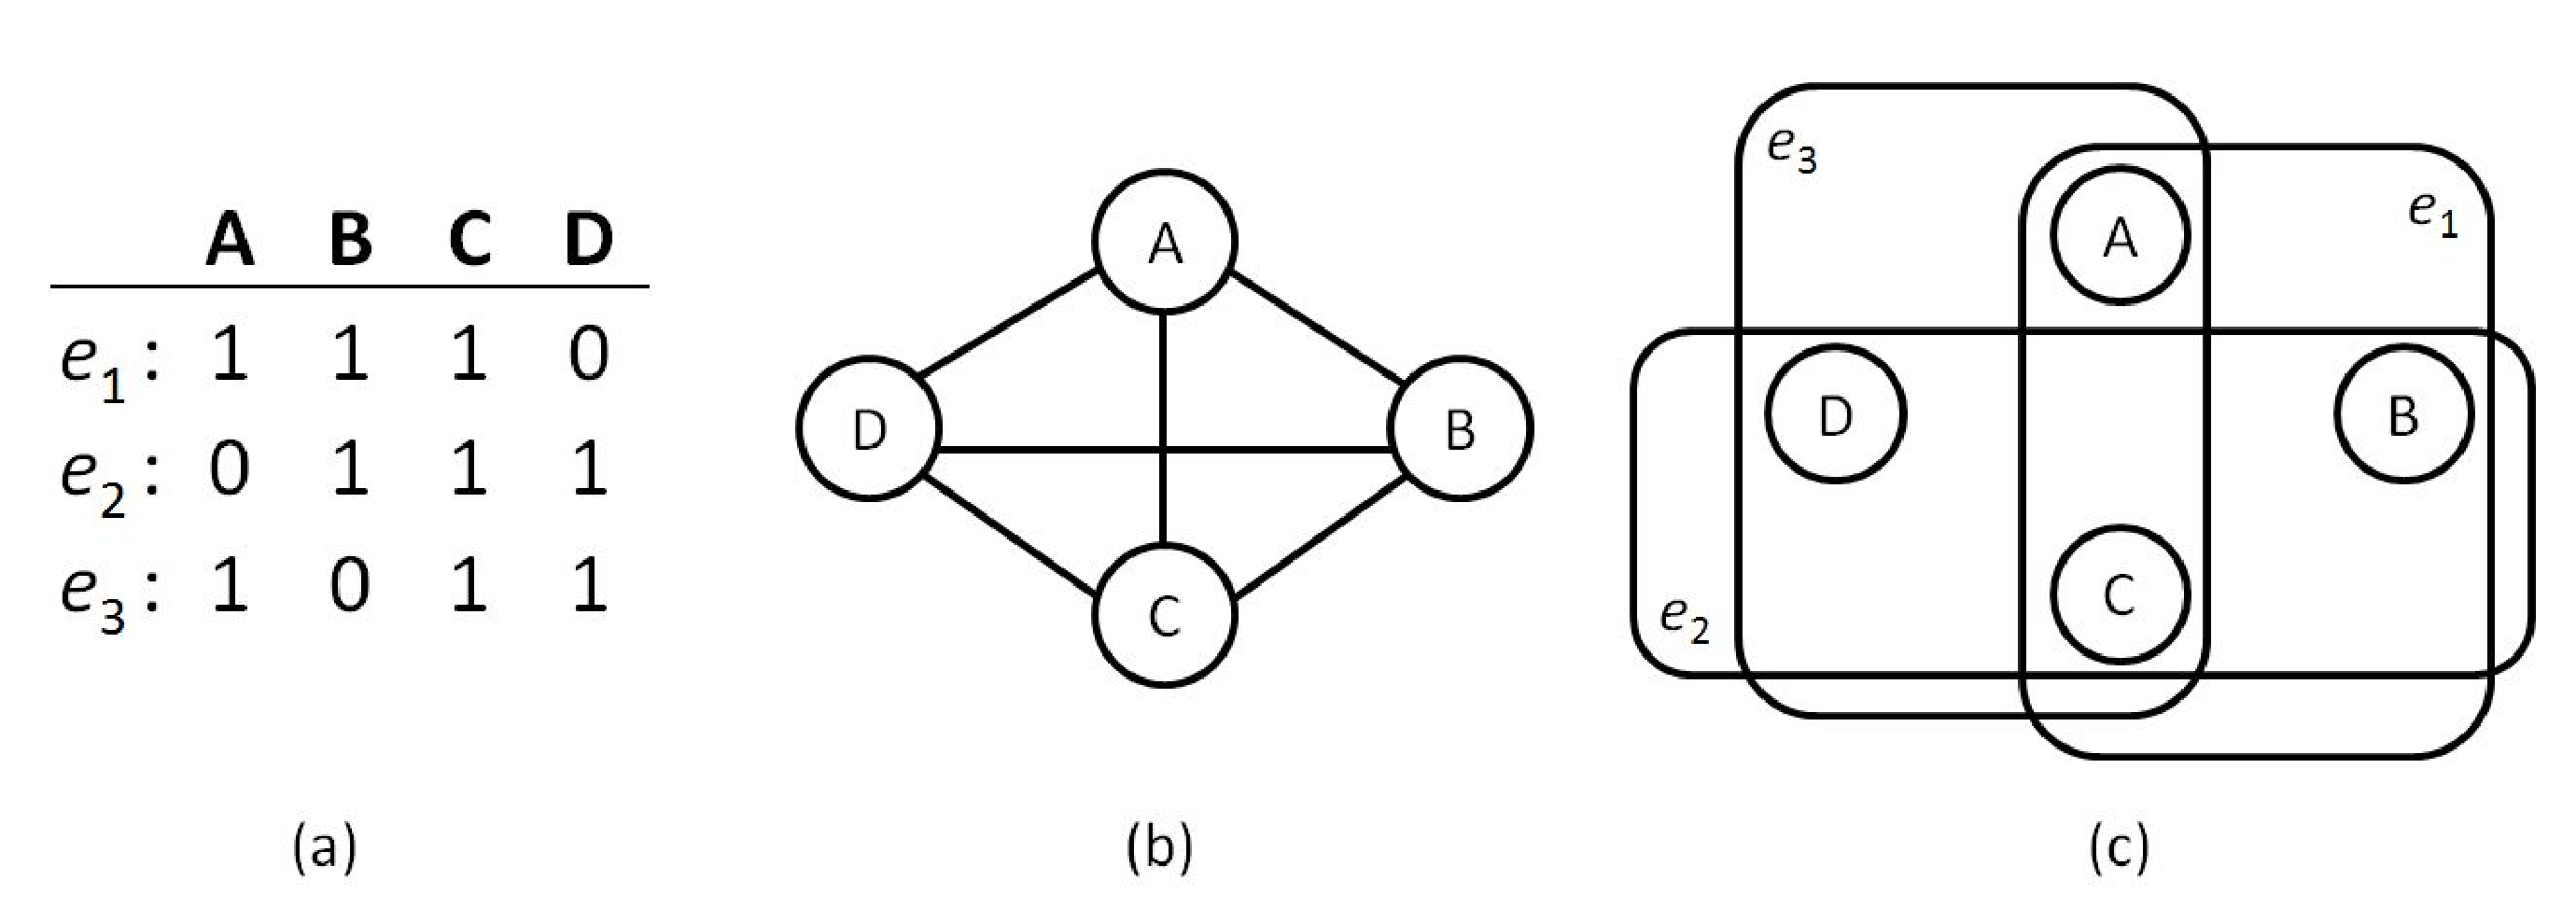
\includegraphics[width=.8\textwidth]{fig/hg_and_rg1.eps}
\end{center}
\caption{\label{fig:hg_and_rg} (a) an example transaction table; (b) the Gaifman graph representation of the table; (c) The hypergraph representation of the table}
\end{figure*}


\subsection{Similarity Measure}
%Sheth et al.~\cite{Sheth05semanticassociation} proposed a formalism for semantic association between entities in an RDF graph. Specifically, the semantic association is defined based on semantic connectivity which indicates if there exists a sequence of interconnected links between two given entities. In our study of semantically associated itemsets in transaction data, the link between entities is essentially the `co-occurrence' relationship. The semantic association according to Sheth et al's definition between transaction items $i_0$ and $i_n$ can be established by identifying a link of the form $i_0, P_c, i_1, P_c, \ldots, i_{n-1}, P_c, i_{n}$, in which $P_c$ denotes the co-occurrence property. The random walk model on hypergraph described in Section~\ref{sec:rw_hyper} formalizes this point of view. Our method for measuring the strength of semantic association is hence based on constructing a hypergraph representation and studying its property with both graph theoretical and spectral analysis techniques.

%Connectivity query between two nodes are essential in numerous mining tasks. Sheth et al.~\cite{Sheth05semanticassociation} defined semantic connectivity in RDF graph as follows. Two entities $e_1$ and $e_n$ are semantically connected if there exists a sequence $e_1, P_1, e_2, P_2, e_3, \ldots, e_{n-1}, P_{n-1}, e_n$ in an RDF graph where $e_i$ are entities and $P_j$ are properties. A sequence of alternating entities and properties represents a semantic path. Fig.~\ref{fig:graphcomp}(B) shows the connectivity between nodes c, a, and e. Paths connecting these nodes are colored in blue.

Given graph-based representation of information sources, meaningful similarity measure $s$ between nodes in the graph is critical in numerous data mining tasks. Take the simple network in Fig.~\ref{fig:graphcomp}(B) for example, suppose given a task of friend recommendation based on the information in this graph, the interesting question is whether $c$ or $e$ is a better choice of recommendation to $a$. To answer this question, it is natural to compare the similarity measures $s(a, c)$ and $s(a, e)$. In a rough sense, on can identify in the hypergraph representation that there are two paths between $a$ and $c$ (the formal definition for paths in hypergraphs will be given in Section~\ref{sec:rw_hyper}), while only one between $a$ and $e$. It's intuitive to conclude that $a$ and $c$ are more similar, or closer, than $a$ and $e$. This gives us a hint that meaningful similarity measures on the graph should satisfy the following intuitions:
\begin{enumerate}
\item The more paths connecting two nodes, the closer they are.
\item The shorter the paths, the closer they are.
\end{enumerate}
In other words, the more ``short" connections between two given nodes, the more similar those nodes are. To this end, we propose to employ the following quantities as the candidate similarity measure since both of them have the desired property. They are, namely, the \emph{commute time distance} based similarity measure from the random walk model on hypergraph, and the inner product similarity based on the \emph{pseudoinverse of the hypergraph Laplacian}. They are all based on the random walk model on hypergraph. In the following, we briefly introduce the theory of random walk.

\subsubsection{Random Walk}
\textbf{Random Walk on Simple Graph}
Given a graph and a starting point we select a neighbor of it at random and move to this neighbor then we select a neighbor of this point at random and move to it etc. The random sequence of points selected this way is a random walk on the graph. In other words, a random walker can jump from vertex to vertex and each vertex therefore represents a state of the Markov chain. The average first-passage time $m(k|i)$~\cite{randomwalks} is the average number of steps needed by a random walker for reaching state $k$ for the first time, when starting from state $i$. The symmetrized quantity $n(i,j)=m(j|i)+m(i|j)$ called the average commute time~\cite{randomwalks}, provides a distance measure between any pair of states. The fact that this quantity is indeed a distance on a graph was proved independently by Klein and Randic~\cite{Klein} and Gobel and Jagers~\cite{Gobel}.

%The average commute time has the nice property of decreasing when the number of paths connecting two vertices increases and when the ``length" of any path decreases, that is, when communication is facilitated. In short, the more short paths connect two given vertices, the more similar those vertices are. The ``shortest path" or ``geodesic" distance does not have the nice property of decreasing when connections between nodes are added: It does not capture the fact that strongly connected nodes are at a smaller distance than weakly connected ones.

The Laplacian matrix $\mathbf{L}$ of a graph is widely used for finding many properties of the graphs in spectral graph theory. Given node degree matrix $\mathbf{D}$ and graph adjacency matrix $\mathbf{A}$, the Laplacian matrix of the graph is defined as $\mathbf{L}=\mathbf{D}-\mathbf{A}$. The normalized Laplacian is given by $\mathbf{L}_N=\mathbf{I}-\mathbf{D}^{-1/2}\mathbf{A}\mathbf{D}^{-1/2}$, where $\mathbf{I}$ is the identity matrix. The average commute time $n(i,j)$ can be computed in closed form from the Moore-Penrose pseudoinverse of $\mathbf{L}$~\cite{pseudo}, denoted by $\mathbf{L}^+$.

Various quantities derived from random walk on graph has been used in a number of applications. Fouss et al.~\cite{Fouss06random-walkcomputation} compared twelve scoring algorithms based on graph representation of the database to perform collaborative movie recommendation. Pan et al.~\cite{Pan} developed a similarity measure based on random walk steady state probability to discover correlation between multimedia objects containing data of various modalities. Yen et al.~\cite{Yen05clusteringusing} introduced a new k-means clustering algorithm utilizing the random walk average commute time distance. Zhou et al.~\cite{Zhou:2009:GCB:1687627.1687709} presented a unified framework based on neighborhood random walk to integrate structural and attribute similarities for graph clustering.

\section{Hypergraph-based Data Mining}
\subsection{Graph-based similarity}
\begin{figure}[tbh]
\centering
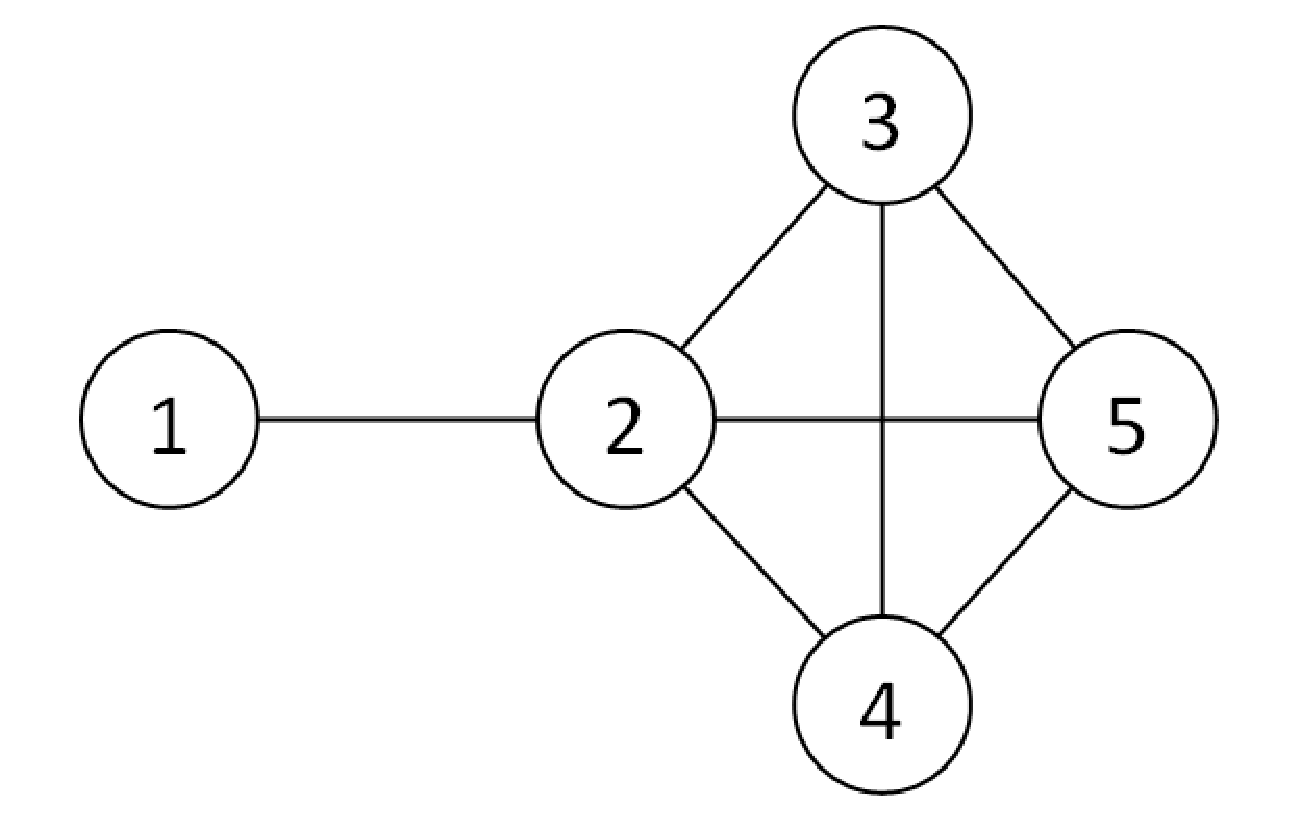
\includegraphics[width=.4\textwidth]{fig/comm-dist-demo.eps}
\caption{\label{fig:comm-dist-demo} .}
\end{figure}

\begin{table}[ht]
\begin{tabular}{r|r|r|r|r|r || r|r|r|r|r}
\hline\hline
\multicolumn{6}{c||}{Euclidian Distance}	&	\multicolumn{5}{c}{Commute Distance}		\\
\hline\hline							
Index	&	1	&	2	&	3	&	4	&	5	&	1	&	2	&	3	&	4	&	5	\\
\hline
1	&	0	&	1	&	1.85	&	1.85	&	2.41	&	0	&	12.83	&	19.79	&	19.79	&	20.34	\\
\hline
2	&	1	&	0	&	1	&	1	&	1.41	&	12.83	&	0	&	6.96	&	6.96	&	7.51	\\
\hline
3	&	1.85	&	1	&	0	&	1.41	&	1	&	19.79	&	6.96	&	0	&	7.51	&	6.96	\\
\hline
4	&	1.85	&	1	&	1.41	&	0	&	1	&	19.79	&	6.96	&	7.51	&	0	&	6.96	\\
\hline
5	&	2.41	&	1.41	&	1	&	1	&	0	&	20.34	&	7.51	&	6.96	&	6.96	&	0	\\
\hline\hline
\end{tabular}
\caption{\label{tbl:comp-eucl-comm} .}
\end{table}
\textbf{Average Commute Time Similarity $s_{CT}$}\\

As already mentioned, the commute-time distance $n(i,j)$ between two nodes $i$ and $j$ has the desirable property of decreasing when the number of paths connecting the two nodes increases and when the length of paths decreases. This is indeed an intuitively satisfying property of the effective resistance of the equivalent electrical network~\cite{Doyle}. The usual shortest-path distance (also called geodesic distance) does not have this property: the shortest-path distance does not capture the fact that strongly connected nodes are closer than weakly connected nodes.

% \subsection{Mining Semantic Associations}
% \label{sec:assoc_noonto}
% \begin{figure}[tbh]
% \centering
% 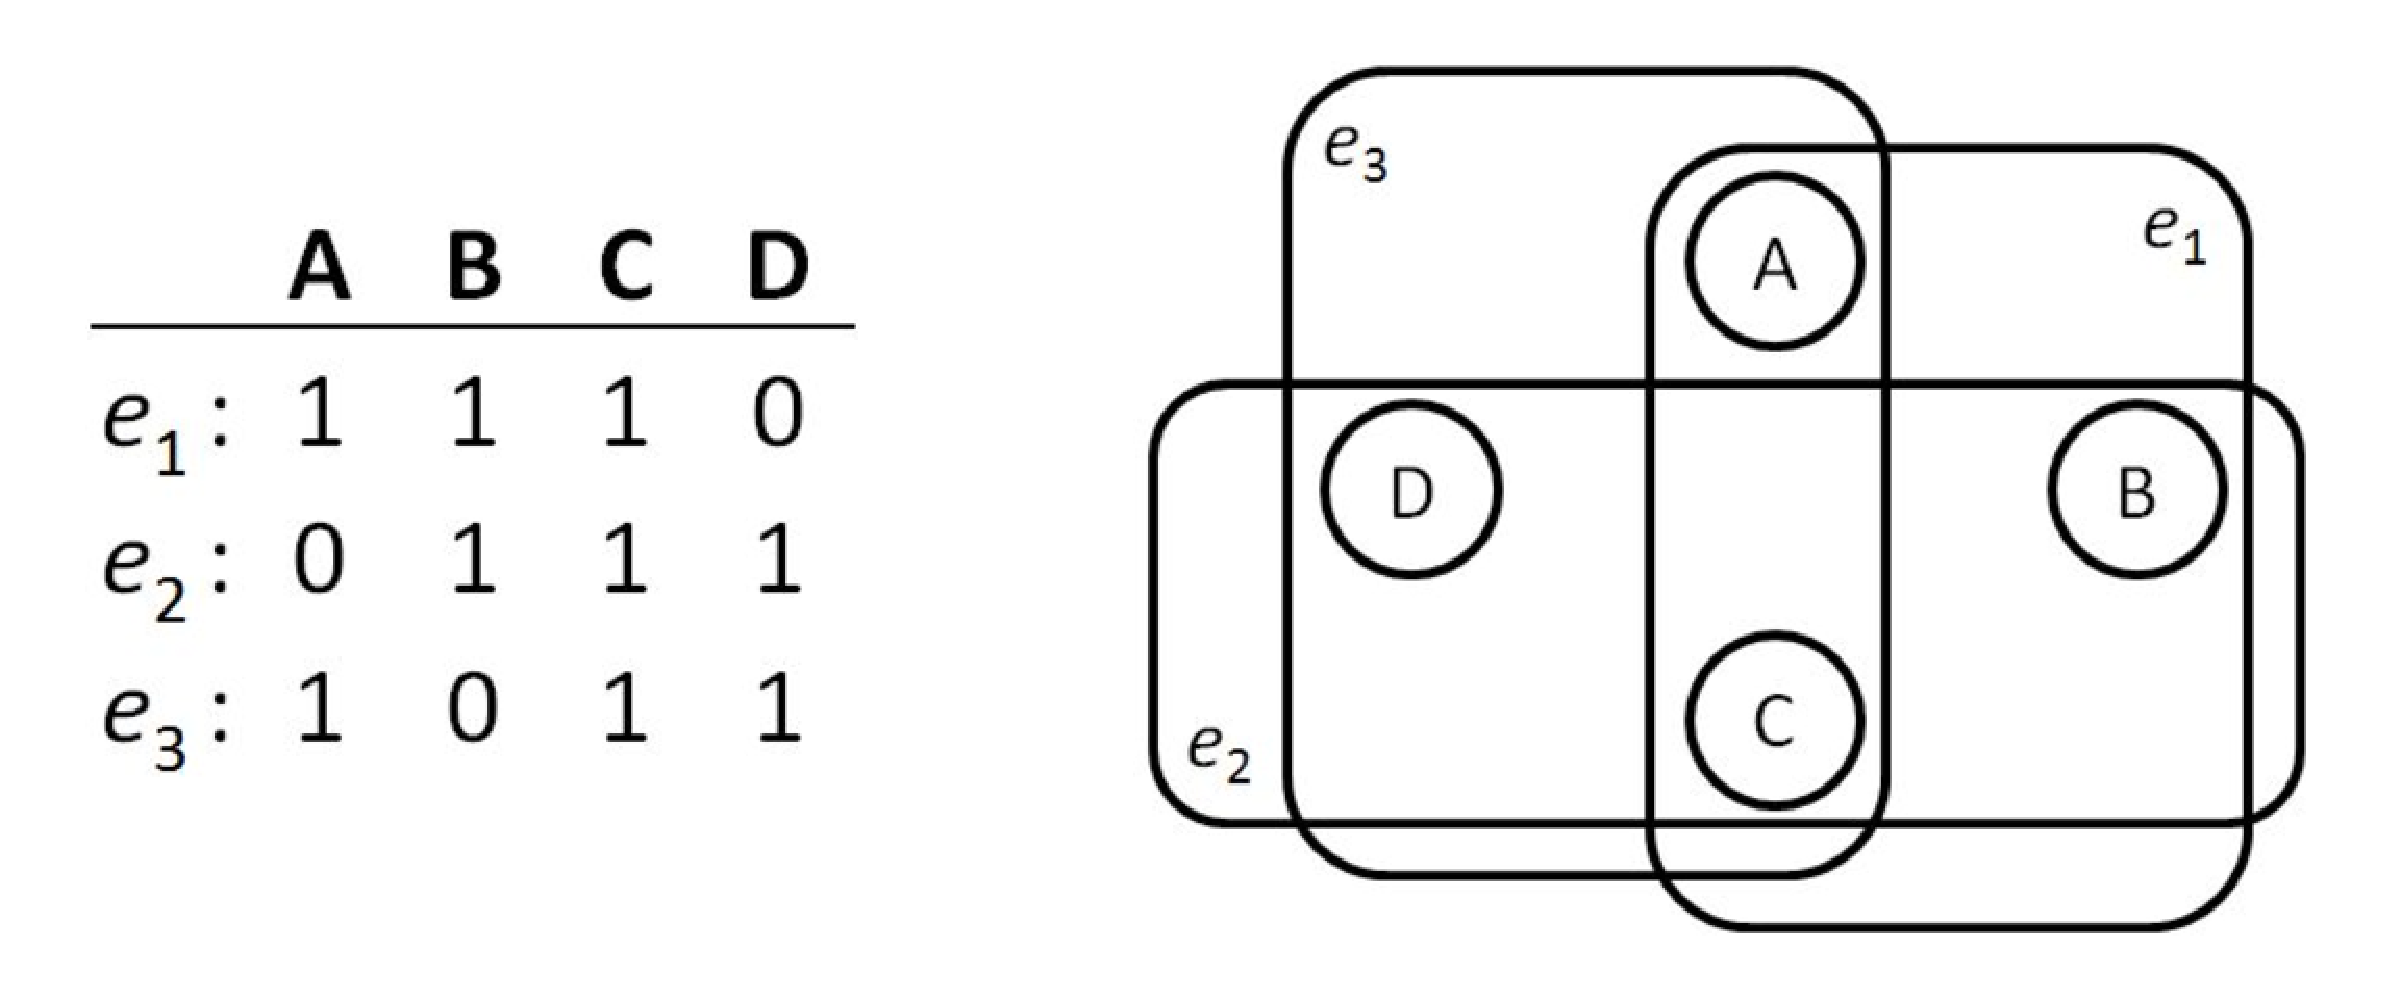
\includegraphics[width=.6\textwidth]{fig/hypergraph-row-wise.eps}
% \caption{\label{fig:hypergraph-row-wise} .}
% \end{figure}

\begin{figure}[tbh]
\centering
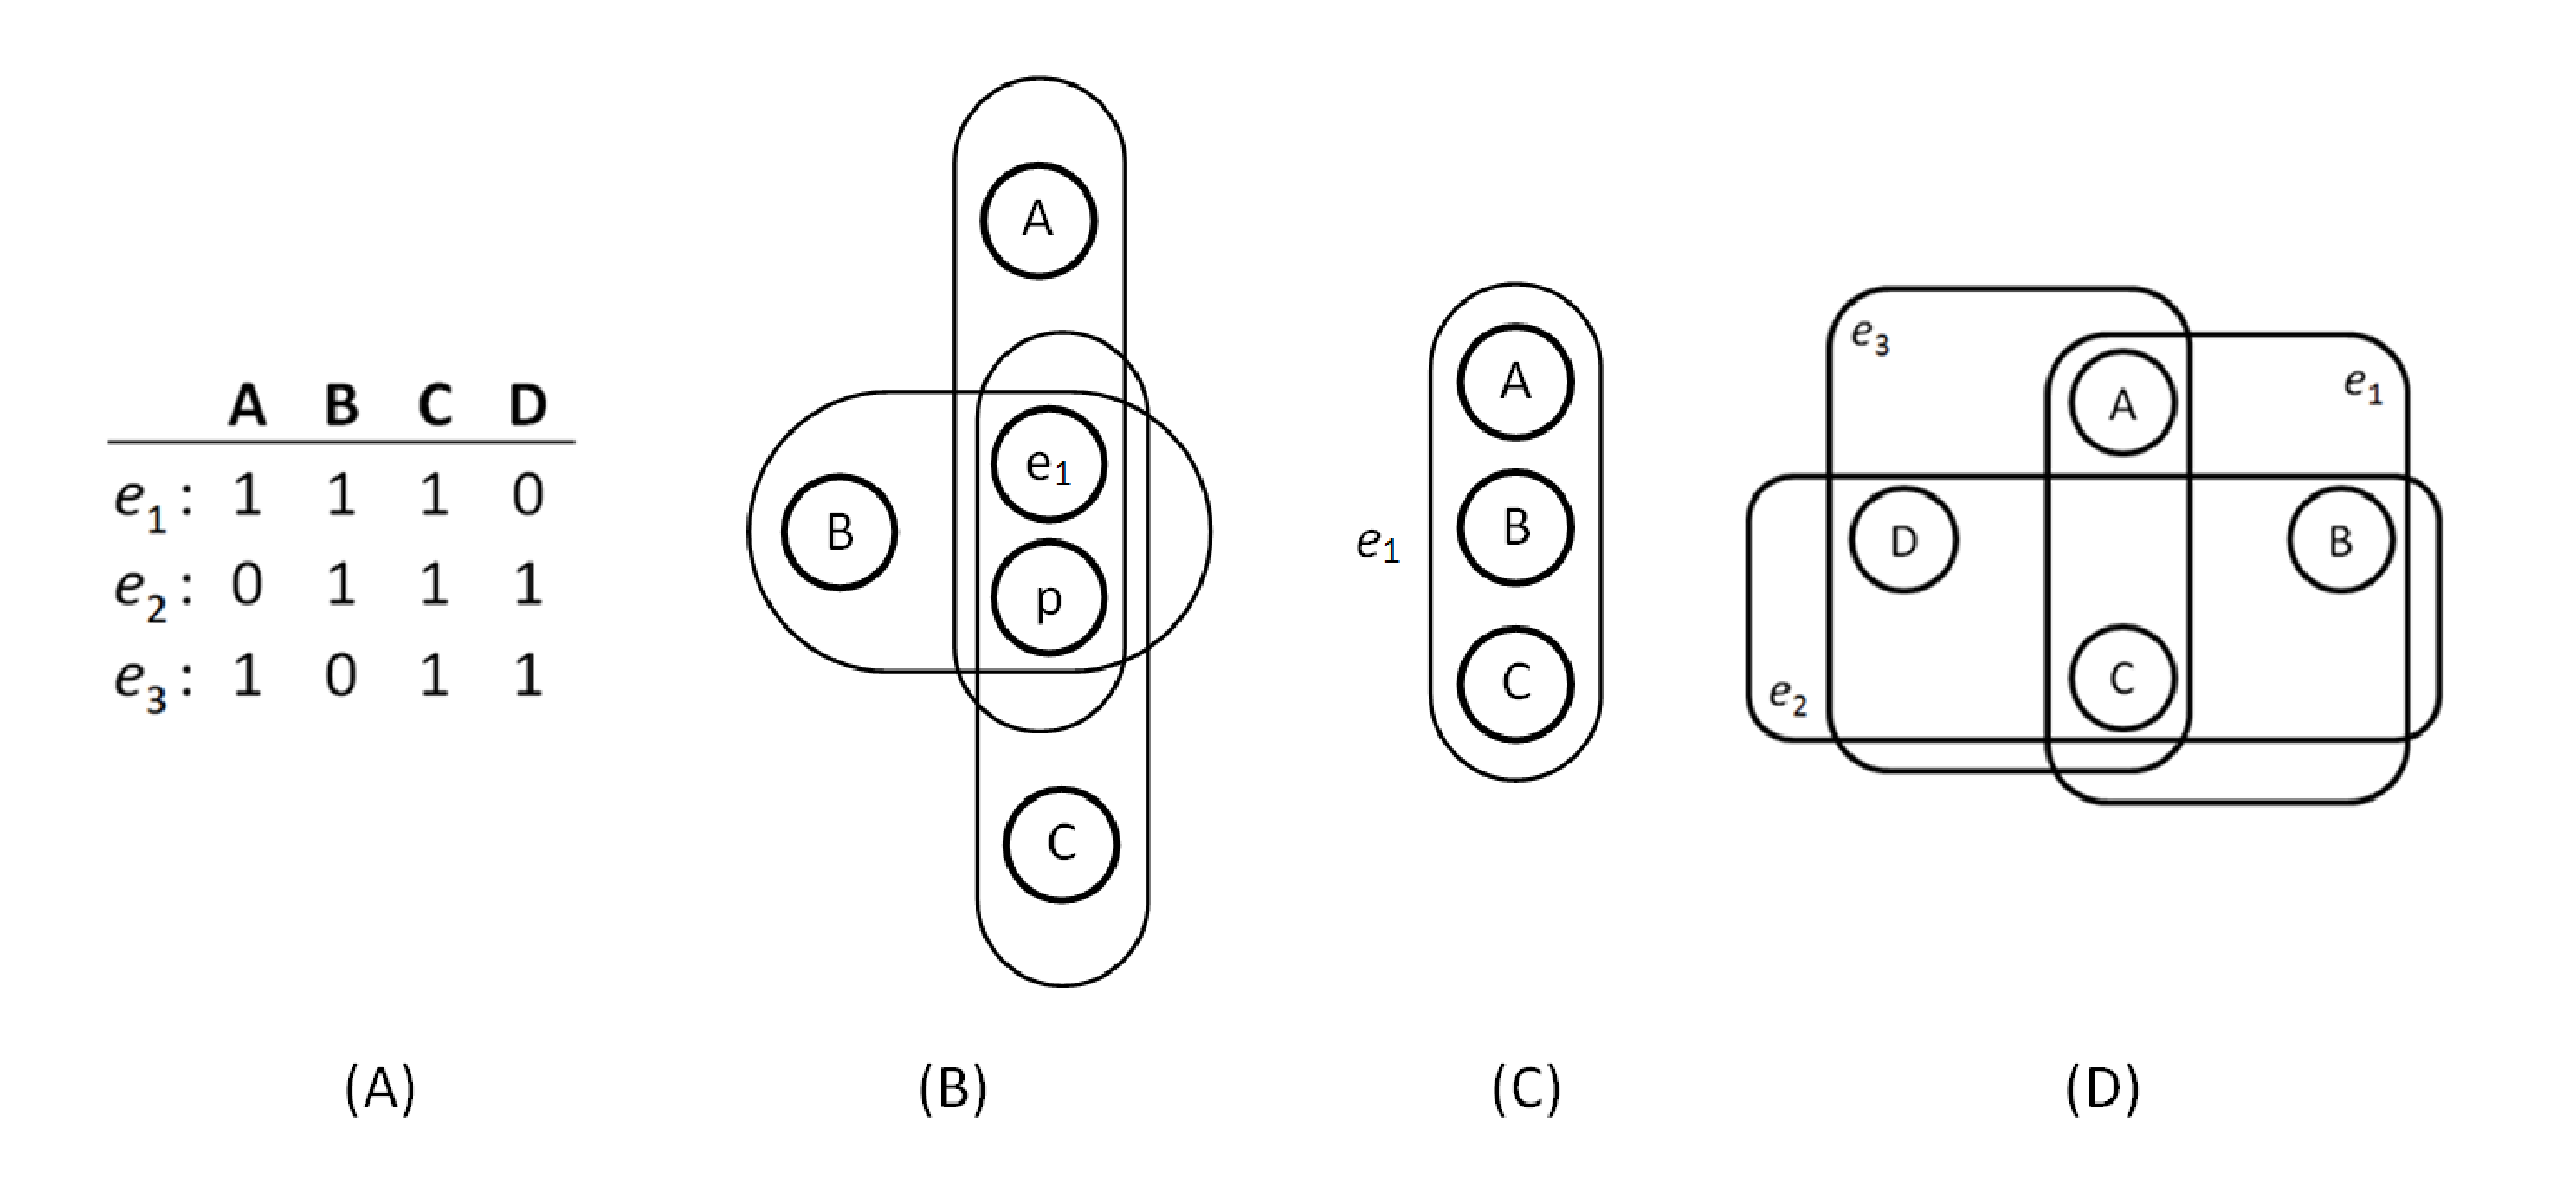
\includegraphics[width=\textwidth]{fig/hypergraph-coarsening.eps}
\caption{\label{fig:hypergraph-coarsening} .}
\end{figure}

If a mining task does not involve the usage of ontologies and focuses only on data in tables, we can use an alternative hypergraph representation that is more compact than the RDF bipartite graph to model the data. The process to generate such hypergraph is called \emph{RDF hypergraph coarsening} as described in Definition~\ref{def:hg-coarsen}.

\begin{mydef}[\textbf{RDF hypergraph coarsening}]
\label{def:hg-coarsen}
RDF hypergraph coarsening is the process of computing a compact form given an input RDF hypergraph for a relational table by merging vertices into larger groups and removing less significant vertices. The choice of vertices is pertinent to the specific mining tasks. Note that RDF hypergraph is 3-uniform and in the case of RDF hypergraph for relation tables, each hyperedge has three nodes corresponding to the RDF statement of the form \texttt{<row>, <p>, <column>}. The \texttt{<p>} node is the auxiliary predicate denoting the context-dependent semantic relationship between the row and column nodes (\eg, such as that can be as general as \texttt{<mentions>}), and since it is incident to all RDF hyperedges it is first removed in the coarsening process as it bears the least amount of information. Next, if the mining task focuses on discovering patterns among column nodes (\eg, frequent pattern mining), we can merge column nodes that coincide with the same row nodes into a new hyperedge and subsequently remove the row node, and vice versa for mining tasks focusing on row nodes.
\end{mydef}

\begin{myexp}[\textbf{Generation of a column-wise hypergraph for a relational table}]
\label{column-wise-hg}
Figure~\ref{fig:hypergraph-coarsening} (A) shows a sample relational table. Using the method described in Example~\ref{exp:repBinRDB} we can represent this binary-valued table to an RDF hypergraph as is shown in Figure~\ref{fig:hypergraph-coarsening} (B), which demonstrates three hyperedges corresponding to the first row in the table created by transforming the row into three RDF statements, i.e., \texttt{<$e_1$, p, A>, <$e_1$, p, B>}, and \texttt{<$e_1$, p, C>}. Figure~\ref{fig:hypergraph-coarsening} (C) illustrates the coarsened hypergraph according to Definition~\ref{def:hg-coarsen}. Supposing we are interested in discovering relationship between column nodes \texttt{A, B} and \texttt{C} in a frequent pattern mining task, we can remove the nodes \texttt{$e_1$} and \texttt{p} that are commonly incident to all the three hyperedges, and then merge nodes \texttt{A, B} and \texttt{C} to form a single hyperedge. Figure~\ref{fig:hypergraph-coarsening} (D) shows the resulting coarsened hypergraph for the relational table in Figure~\ref{fig:hypergraph-coarsening} (A).
\end{myexp}

In this section, we present our preliminary study for discovering semantically associated itemsets based on hypergraph. The goal of this study is to show that, using graph based formalism, we can obtain interesting patterns that are unable to be captured by traditional methods. Specifically, we propose to construct a hyperedge for each tuple. The relational attributes constitute the universe of vertices in the hypergraph. Given the hypergraph representation of relational structure, our approach starts by first generating semantically associated 2-itemsets. A 2-itemset $\langle i,j \rangle$ is considered semantically associated if the hypergraph-based similarity measure $s(i,j)$ exceeds some threshold. In the following subsections, we propose two similarity measures $s_{CT}$ and $s_{L+}$ based on, respectively, the average commute time distance on hypergraph and the inner-product-based representation of the pseudoinverse of Hypergraph Laplacian. Given discovered semantically associated 2-itemsets, we propose a hypergraph expansion method along with two search strategies, namely, the clique and connected component search, in the resulting graph for finding semantically associated $k$-itemsets ($k>2$).

\textbf{Random Walk on Hypergraph}
\label{sec:rw_hyper}
We can associate each hypergraph with a natural random walk which has the transition rule as
described in~\cite{Zhou06learningwith}. Given the current position $u \in V$; first choose a hyperedge $e$ over all hyperedges
incident with $u$ with the probability proportional to $w(e)$; and then choose a vertex $v \in e$
uniformly at random. Obviously, it generalizes the natural random walk defined on simple
graphs. Let $\mathbf{P}$ denote the transition probability matrix of this hypergraph random walk.
Then each entry of $\mathbf{P}$ is
\[
p(u,v) = \sum_{e\in E}{w(e)\frac{h(u,e)}{d(u)}\frac{h(v,e)}{\delta(e)}}\, .
\]
In matrix notation, $\mathbf{P}=\mathbf{D}_v^{-1}\mathbf{HWD}_e^{-1}\mathbf{H}^T$.
Zhou et al.~\cite{Zhou06learningwith} define the following normalized hypergraph Laplacian $\mathcal{L}$ based on the random walk model:
\begin{align}
\mathcal{L}=\mathbf{I}-\mathbf{\Theta},   ~\mathrm{where}~ \mathbf{\Theta}=\mathbf{D}_v^{-\frac12}\mathbf{HWD}_e^{-1}\mathbf{H}^T\mathbf{D}_v^{-\frac12} \label{eq:normalizedHyperL}.
\end{align}

\subsubsection{Methods for Generating 2-itemsets}
In the following we describe two similarity measures that define the strength of bond between a pair of semantically associated items.

To compute commute-time distance between vertices in a hypergraph, we need to first define the combinatory hypergraph Laplacian $\mathbf{L}$.
It follows from Zhou et al's formalism of normalized hypergraph Laplacian in Equation~\ref{eq:normalizedHyperL} that:
\begin{equation}
\mathbf{L}=\mathbf{D}^{1/2}\mathcal{L}\mathbf{D}^{-1/2}=\mathbf{D}_v-\mathbf{HWD}_e^{-1}\mathbf{H}^T \label{eq:combinatoryHyperL}
\end{equation}

The average commute time $n(i,j)$ on simple graph can be computed in closed form from the Moore-Penrose pseudoinverse of $\mathbf{L}$ ~\cite{pseudo}, denoted by $\mathbf{L}^+$ with elements $l_{ij}^+=[\mathbf{L}^+]_{ij}$. It can be shown that $n(i,j)$ on hypergraph can be calculated in the same manner. The pseudoinverse $\mathbf{L}^+$ is given by the following equation:
\begin{equation}
\mathbf{L}^+=(\mathbf{L} -\mathbf{ee}^T/n)^{-1} + \mathbf{ee}^T/n, \label{eq:pL}
\end{equation}
where $\mathbf{e}$ is a column vector made of 1s (i.e., $\mathbf{e}=[1,1,\ldots,1]^T$). The formula for the computation of $n(i,j)$ takes the form of the following equation:
\begin{equation}
n(i,j)=V_G(l_{ii}^+ + l_{jj}^+ - 2l_{ij}^+) \label{eq:CT},
\end{equation}
where $V_G = tr(\mathbf{D}_v)$ is the volume of the hypergraph. If we define $\mathbf{e}_i$ as the $i$th column of $\mathbf{I}$ (i.e.,
$
\mathbf{e}_i=[\stackbin[1]{}{0}, \ldots, \stackbin[i-1]{}{0}, \stackbin[i]{}{1},$
$ \stackbin[i+1]{}{0}, \ldots, \stackbin[n]{}{0}]^T
$),
Equation~\ref{eq:CT} can be transformed to:
\begin{align}
n(i,j)=V_G(\mathbf{e}_i-\mathbf{e}_j)^T\mathbf{L}^+(\mathbf{e}_i-\mathbf{e}_j), \label{eq:CT2}
\end{align}
Since $n(i,j)$ is a distance, it is straightforward to convert it to a similarity measure $s_{CT}(i,j)$ by normalize it to unit range and subtract from 1.

\textbf{Pseudoinverse-based Inner-Product Similarity $s_{L+}$}\\
Equation \ref{eq:CT2} can be mapped into a new Euclidean space that preserves the commute time distance:
\begin{align}
\notag n(i,j)&=V_G(\mathbf{e}_i-\mathbf{e}_j)^T\mathbf{L}^+(\mathbf{e}_i-\mathbf{e}_j)\\
\notag &=V_G(\mathbf{x}_i'-\mathbf{x}_j')^T(\mathbf{x}_i'-\mathbf{x}_j')\\
&=V_G\|\mathbf{x}_i'-\mathbf{x}_j'\|^2, \label{eq:ECTD}
\end{align}
where $\mathbf{x}_i'=\mathbf{\Lambda}^{1/2}\mathbf{U}^T\mathbf{e}_i$, $\mathbf{U}$ is an orthonormal matrix made of eigenvectors of $\mathbf{L}^+$ (ordered in decreasing order of corresponding eigenvalue $\lambda_k$) and $\mathbf{\Lambda}=\mathbf{Diag}(\lambda_k)$. In this way, the transformed node vectors $\mathbf{x}_i'$ are exactly separated in the new $n$-dimensional Euclidean space.
From this definition, it follows that $\mathbf{L}^+ $ is the matrix containing inner products of the transformed vectors $\mathbf{x}_i'$ as shown below:
\begin{align}
\notag \mathbf{x}_i'^T\mathbf{x}_j'&=(\mathbf{\Lambda}_i^{1/2}\mathbf{x}_i)^T\mathbf{\Lambda}_j^{1/2}\mathbf{x}_j=\mathbf{x}_i^T\mathbf{\Lambda}\mathbf{x}_j\\
&=\mathbf{e}_i^T\mathbf{U\Lambda U}^T\mathbf{e}_j=\mathbf{e}_i^T\mathbf{L}^+\mathbf{e}_j=l_{ij}^+.
\end{align}
Therefore, $\mathbf{L}^+$ can be considered as a similarity matrix for the nodes---that is
\begin{equation}
s_{L^+}(i,j)=l_{ij}^+ \, . \label{eq:sim_L+}
\end{equation}
The inner-product-based similarity measures are well-studied for the vector-space model of information retrieval. It has been shown that when computing proximities between documents, inner-product-based measures outperform Euclidean distances~\cite{IR}.

\subsubsection{Effective Computation}
\label{sec:eff_comp}
In high dimensional data sets, the computations of the Hypergraph Laplacian and the pseudoinverse becomes intractable. We discuss two approaches to mitigate this scalability problem.

To compute Hypergraph Laplacian $\mathbf{L}$ in Equation \ref{eq:combinatoryHyperL} requires multiplication of hypergraph incidence matrices $\mathbf{H}$ and its transpose $\mathbf{H}^T$. Since $\mathbf{H}$ grows in proportion to the size of underlying transaction data (each node corresponds to a column and each hyperedge corresponds to a row), it eventually becomes unable to fit in memory when the size exceeding a certain amount. In this case the computation can still be carried out using a block partitioned matrix product by performing operations only on the submatrices of tractable sizes. Owing to the fact that, in most cases, $|V|$ is much smaller than $|E|$, $\mathbf{H}$ can then be partitioned into $s$ vertical stripes and the square matrix $\mathbf{D}_e$ into $s$ diagonal blocks. The multiplication in Equation \ref{eq:combinatoryHyperL} can be calculated by $\mathbf{HD}_e^{-1}\mathbf{H}^T=\sum_{\gamma=1}^s{\mathbf{H}_\gamma\mathbf{D}_{e\gamma}^{-1}\mathbf{H}_\gamma^T}$. Note that $\mathbf{H}$ is sparse in many applications. This property can be exploited to gain high performance and due to its importance much effort has been devoted to the study resulting a number of libraries and routines from which we can leverage.

As the number of nodes grows, to compute pseudoinverse in closed form using Equation \ref{eq:pL} also becomes intractable. A procedure based on Cholesky factorization to compute $\mathbf{L}^+$ for large sparse matrices~\cite{matrix} is proved useful. It allows to compute $\mathbf{L}^+$ in a column-by-column manner. In particular, the procedure involves the following steps for computing the $i$th column of $\mathbf{L}^+$:
\begin{enumerate}
\item Compute the projection $\mathbf{y}_i$ of base vector $\mathbf{e}_i$ on the column space of $\mathbf{L}$.
\item Find a solution $l_i^{*+}$ of the linear system $\mathbf{Ll}=\mathbf{y}_i$.
\item Project $l_i^{*+}$ on the row space of $\mathbf{L}$ to get $l_i^+$.
\end{enumerate}
Since $\mathbf{L}$ is symmetric, its row space is the same as column space. The projection in step 1 and 2 can be represented by the matrix $(\mathbf{I-ee}^T/n)$. The equation in step 2 can be solved by first solving a reduced linear system: $\mathbf{\hat{L}\hat{l}}=\mathbf{\hat{y}}_i$, where $\mathbf{\hat{L}}$, $\mathbf{\hat{l}}$, and $\mathbf{\hat{y}}$ are obtained respectively by removing the last row from $\mathbf{l}$, $\mathbf{y}$, and last row and column from $\mathbf{L}$. We observe that $\mathbf{\hat{L}}$ is full rank and positive definite and hence is able to be decomposed using the Cholesky factorization, $\mathbf{\hat{L}=RR}^T$. Since $\mathbf{R}$ is lower-triangular, one solution of $\mathbf{\hat{L}\hat{l}}=\mathbf{RR}^T\mathbf{\hat{l}}=\mathbf{\hat{y}}_i$ can be efficiently obtained by two back-substitutions. After solving the reduced linear system, the solution to the original equation in step 2 is therefore $(\mathbf{l}_i^{*+})=[\mathbf{\hat{l}}_i^{*+},0]^T$. With the help of this technique, we are able to analyze datasets of a million rows and 10 thousand columns.


\subsubsection{Methods for Generating $k$-itemset ($k>2$)}
Now, we consider finding semantically associated $k$-itemset ($k>2$) from given 2-itemsets.
As is common in hypergraph theory, we can associate an induced graph $G(H)$ with every hypergraph $H$ by expanding every hyperedge $e$ in $H$ to a clique in $G(H)$. Edges in the induced graph $G(H)$ can be called \emph{subedges} to avoid unnecessary confusion. We can further construct a pruned graph $G'(H)$ from $G(H)$ by applying the following inclusion rule on each subedge: the similarity between the incident nodes of a subedge has to be greater than a user-specified threshold $\theta$. In formal definition, given a hypergraph $H=(V,E)$, the pruned subgraph is $G'(H)=\{V,E'\}$ where
\begin{align}
\notag E'=\{&(u,v)\in V^2 \, : \, u \neq v \; \mathrm{and} \; \\
\notag &u, v \in e \; \mathrm{for} \; \mathrm{some} \; e \in E \; \mathrm{and} \; \\
\notag &s(u,v) > \theta\}.
\end{align}
Given $G'(H)$, finding semantically associated $k$-itemset ($k>2$) can be formulated into two ways: finding cliques or connected components in $G'(H)$.

\subsubsection{Cliques of $G'(H)$}
Finding cliques in $G'(H)$ corresponds to searching and testing in the powerset of $V$. Given the fact that every subset of a clique is also a clique, this downward-closure property can make efficient clique discovery algorithm possible in a way similar to the Apriori algorithm for finding frequent itemsets
--- with a ``bottom up" manner, the candidate generation step extends valid $k-1$ length itemsets one item at a time, and groups of candidates are tested against $G'(H)$ to determine if they form cliques. The algorithm terminates when no further successful extensions are found.

\subsubsection{Connected Components of $G'(H)$}
Complete subgraph (i.e., clique) is a very strong requirement that can limit the approach to restricted cases of semantically associated itemsets. One way to relax this requirement is to find connected components of $G'(H)$, which can be viewed as a closure under semantic association. The number of connected components equals the multiplicity of 0 as an eigenvalue of the Laplacian matrix of $G'(H)$. Although the set of connected components is not downward closed, there is efficient way to find all connected components of a graph in linear time using either breadth-first search or depth-first search. In either case, a search that begins at some particular vertex will find the entire connected component containing the vertex. When the search returns, loop through other vertices and start a new search whenever the loop reaches a vertex that has not already been included in a previously found connected component.

\subsubsection{Ranking of Itemsets}
Once the semantically associated 2-itemsets and $k$-itemsets are generated, they can be ranked by a quantity indicating the strength of association among items in the set. We tentatively compute this quantity by averaging the total pairwise similarities over the number of subedges of the itemset's corresponding clique or connected component in $G'(H)$.



\section{Incorporation of Ontologies}

Graphs are mathematical objects that enjoy wide-spread usage for many tasks, which include the visualization and analysis of data for humans, mathematical reasoning, and the implementation as a data structure for developing data mining algorithms. Besides the common graph-theoretic model of RDF as labeled, directed multi-graphs, Hayes has established that RDF can be also represented as hypergraphs (bipartite graphs)~\cite{GraphModelRDF}. This result constitutes an important aspect of the theoretical basis of this paper and is discussed in sections below. We propose to use the graph-based representation for RDF as a combined information source of both domain knowledge and data for mining semantic associations.

We distinguish paths in the RDF bipartite graph by assigning weights to those paths that represent different semantic relationships such as class subsumption, part\_of, and other general or domain--specific properties.

\begin{mydef}
\emph{\textbf{(Data model for the combined RDF bipartite graph)}} The unified RDF bipartite graph of both data and ontology is defined as $G=\langle V_v \cup V_s, E \rangle$, where $V_v$ denotes value nodes corresponding to RDF components (subject, predicate, or object), and $V_s$ denotes statement nodes corresponding to RDF statements. More specifically, statement nodes can be further divided according to whether they are from data or ontology, i.e., $V_s=V_d \cup V_o$; the value nodes can be divided according to whether they represent rows or attributes in the data, i.e. $V_d=V_r \cup V_a$. The graph $G$ can be represented in a biadjacency matrix $\mathbf{M}$, where $\mathbf{M}(i,j)$ is non-zero if there is an edge between $\langle V_{v_i}, V_{s_j} \rangle$. For an unweighted graph, the value can be 0/1, while for a weighted graph, any non-negative value.
\end{mydef}

The biadjacency matrix $\mathbf{M}$ can be split into vertical stripes by statement nodes $V_s$. For example, according to Figure~\ref{fig:hypergraph-combined}(B), the bipartite graph corresponding to lower 8 RDF statements representing the underlying transaction table can be modeled as the matrix $\mathbf{M}_d$ in Equation~\ref{eq:Md} (RDF statement nodes are labeled $s_1\dots s_8$ respectively); and the bipartite graph corresponding to upper 4 statements (labeled $s_9\dots s_{12}$) representing the subsumption hierarchy in the ontology can be modeled as the matrix $\mathbf{M}_o$ in Equation~\ref{eq:Mo}.

To obtain the biadjacency matrix $\mathbf{M}$ of the combined RDF bipartite graph in Figure~\ref{fig:hypergraph-combined}, we can simply concatenate $\mathbf{M}_d$ and $\mathbf{M}_o$ horizontally: $\mathbf{M}=\left[\mathbf{M}_d~\mathbf{M}_o\right]$. In general, If there are $k$ different semantic relationships in the ontology, $\mathbf{M}_o$ can be further divided into more vertical stripes $\mathbf{M}_{o_i}, i=1\dots k$, where $\mathbf{M}_{o_i}$ may represent, for example, the ``part\_of" lattice. Each $\mathbf{M}_{o_i}$ is  distinguished from another by the respective weight. In this case, $\mathbf{M}$ is the horizontal concatenation of all the weighted vertical stripes as shown in Equation~\ref{eq:horzcat}. After the concatenation, $\mathbf{M}$ can be represented as the form shown in Equation~\ref{striped_M}.

%horizontal concatenation
\begin{equation}\label{eq:horzcat}
\mathbf{M} = \bigg[w_d\mathbf{M}_d ~~ w_{o_1}\mathbf{M}_{o_1} ~~ w_{o_2}\mathbf{M}_{o_2} ~~ \dots\bigg]
\end{equation}

\begin{equation}\label{eq:Md}
\mathbf{M}_d=\begin{blockarray}{cccccc}
                  ~     &  s_1  &  s_2  &  s_3  & \dots &  s_8  \cr
            \begin{block}{c[ccccc]}
                 r_1    &   1   &   1   &   0   &\multirow{4}{*}{\dots} &   0   \cr
                 r_2    &   0   &   0   &   1   &       &   0   \cr
                 r_3    &   0   &   0   &   0   &       &   0   \cr
                 r_4    &   0   &   0   &   0   &       &   1   \cr
                 %\cline{1-6}
                  A     &   1   &   0   &   1   &\multirow{4}{*}{\dots} &   0   \cr
                  B     &   0   &   1   &   0   &       &   0   \cr
                  C     &   0   &   0   &   0   &       &   0   \cr
                  D     &   0   &   0   &   0   &       &   1   \cr
                  E     &   0   &   0   &   0   &       &   0   \cr
            \end{block}
        \end{blockarray}
\end{equation}
\begin{equation}\label{eq:Mo}
\mathbf{M}_o=\begin{blockarray}{ccccc}
            \begin{block}{c[cccc]}
                  ~     &  s_9  & s_{10}& s_{11}& s_{12}\cr
                 r_1    &   0   &   0   &   0   &   0   \cr
                 r_2    &   0   &   0   &   0   &   0   \cr
                 r_3    &   0   &   0   &   0   &   0   \cr
                 r_4    &   0   &   0   &   0   &   0   \cr
%                 \cline{1-5}
                  A     &   1   &   0   &   0   &   0   \cr
                  B     &   0   &   1   &   0   &   0   \cr
                  C     &   1   &   1   &   1   &   0   \cr
                  D     &   0   &   0   &   0   &   1   \cr
                  E     &   0   &   0   &   1   &   1   \cr
            \end{block}
        \end{blockarray}
\end{equation}




\begin{equation}
\label{striped_M}
\mathbf{M}=\begin{blockarray}{ccccc}
                ~ & ds & os_1 & os_2 & \dots \\
            \begin{block}{c[c|c|c|c]}
                r   &   \mathbf{M}_{dr}  &   \mathbf{0}   &   \mathbf{0}   &   \dots \\
                \cline{2-5}
                a   &   \mathbf{M}_{da}  &   \mathbf{O}_1 &   \mathbf{O}_2 &   \dots \\
            \end{block}
        \end{blockarray}
\end{equation}

By developing the unified representation for both data and domain knowledge, and utilizing ontology annotations, such as our results~\cite{LePendu2010}, we can produce one RDF hypergraph, which serves as the basis for perform semantic data mining in a systematic way. Given this, the main research challenge is how to utilize the data and ontology together for semantic data mining. In this paper, we focus on one fundamental data mining tasks, namely, the {\em association mining}. With additional information from ontology (domain knowledge), the unified RDF hypergraphs will enable us to discover hidden association between entities, between entities and ontological concepts, and between ontological concepts. Intuitively, these associations are defined in terms of the paths linking the nodes and the node labels should be taken into consideration as they represent different semantics.



\subsection{Similarity Ranking by Random Walk with Restart}

Similar to the relevance score~\cite{SunEtal05}, we believe that two items have a strong semantic association if they are related to many similar objects. We denote the similarity score between entities $e_1$ and $e_2$ by $s(e_1, e_2)$, where $s(e_1,e_2) \in [0, 1]$ and $s(e_1, e_2) = 1 \text{ if } e_1 = e_2$. Now the problem of ranking semantic associations in the unified graph can be described as follows:

Given an attribute node $a$ in the unified graph $G = G_d \cup G_o$ and $a \in G_d \cap G_o$ we want to compute a similarity score $s(a, b)$ for all nodes $b(\neq a) \in G_d \cap G_o$. The result is a one-column vector containing all similarity scores of the entities with respect to $a$~\cite{Chen_tuplerank:ranking}. The motivation is to apply random walks with restart (RWR) from the given node $a$, and use the steady-state probability of each node at convergence as the similarity measure, i.e., the similarity score of node $b$ is defined as the probability of visiting $b$ via a random walk which starts from $a$ and goes back to $a$ with a probability $c$. In more detail, RWR in a bipartite graph works as follows: assume we have a random walker that starts from node $a$. For each step, the walker chooses randomly among the available edges from the current node it stays. After each iteration, with probability $c$, it resets its position back to node $a$. The final steady-state probability that the random walker reach node $b$ is the similarity score of L with respect to $a$: $s(a, b)$. We choose the random walk approach to compute the relevance score because it gives node $b$ high ranking if $b$ and $a$ are connected by many nodes; this is because the random walker has more paths to reach $b$ from $a$. The purpose of the periodic restart of the random walk is to raise the chance that close related nodes are visited more often than other nodes.

In the following, we first propose an algorithm for random walk-based similarity ranking on a unified RDF bipartite graph. The algorithm can be used in such situations as, for example, if users are interested in products that are usually bought together in the same transactions by different customers, or common side effects of the same drugs prescribed to different patients, etc.

Given the biadjacency matrix $\mathbf{M}$ in Equation~\ref{eq:horzcat} for the combined RDF bipartite graph $G$, we can construct the adjacency matrix $\mathbf{A}$ of $G$ as following:
\[
\mathbf{A}=\left[
               \begin{array}{cc}
                 \mathbf{0}   & \mathbf{M} \\
                 \mathbf{M}^T & \mathbf{0} \\
               \end{array}
             \right]
\]
The probability of a random walker taking a particular edge $\langle a,b\rangle$ from a node $a$ while traversing the graph is proportional to the edge weight over the total weight of all outgoing edges from $a$, i.e., $P(a,b)=A(a,b)/\Sigma_{i=1}^{m+n}A(a,i)$. Therefore, the Markov transition matrix $P$ of $G$ is constructed as: $P=normc(A)$, where $normc(A)$ normalizes $A$ such that every column sum up to 1.

First, we transform the input attribute node $a$ into a $(k+n) \times 1$ query vector $\mathbf{q}_a$ with 1 in the $a$-th row and 0 otherwise. Second, we need to compute the $(k+n)\times 1$ stead-state probability vector $\mathbf{u}_a$ over all nodes in $G$. Last we extract the probabilities of the row nodes as the similarity score vectors. Note that $\mathbf{u}_a$ can be computed by an iterated method from the following lemma.

\begin{mylem}\label{lem:pi}
Let $c$ be the probability of restarting random-walk from the node $a$. Then the steady-state probability vector $\mathbf{u}_a$ satisfies
\begin{equation}
\mathbf{u}_a=(1-c)P_A\mathbf{u}_a+c\mathbf{q}_a~.
\end{equation}
\end{mylem}

\renewcommand{\algorithmicrequire}{\textbf{Input:}}
\renewcommand{\algorithmicensure}{\textbf{Output:}}
\begin{algorithm}
\caption{Calculate Semantic Association}
\label{alg1}
\begin{algorithmic}
\REQUIRE query attribute $a$, bipartite matrix $M$, restarting probability $c$, tolerant threshold $\epsilon$
\ENSURE $y = x^n$
\STATE $\mathbf{q}_a \Leftarrow \mathbf{0}$
\STATE $\mathbf{q}_a(a)=1$ (set $a$-th element of $\mathbf{q}_a$ to 1)
\WHILE{$|\Delta\mathbf{u}_a| > \epsilon$}
\STATE \[
    \mathbf{u}_a = (1-c)  \left[ \begin{array}{c}
        normc(\mathbf{M})\mathbf{u}_a(k+1:k+n);\\
        normc(\mathbf{M}^T)\mathbf{u}_a(1:k)
    \end{array} \right] + c\mathbf{q}_a
\]
\ENDWHILE
\RETURN $\mathbf{u}_a(1:k)$
\end{algorithmic}
\end{algorithm}

The iterative update of $\mathbf{u}_a$ in the algorithm (inside the while loop) is modified from Lemma~\ref{lem:pi} while avoiding materializing $\mathbf{A}$ and $\mathbf{P}$ for scalability.



%%%%%%%%%%%%%%%%%%%%%%%%%%%%%%%%%%%%%%%%%%%%%%%%%%%%%%%%%%%%%%%%%%%

%\chapter{INCORPORATION OF PRIOR KNOWLEDGE}
%\label{chap:incorpont}
%\section{Incorporation of Ontologies}

Graphs are mathematical objects that enjoy wide-spread usage for many tasks, which include the visualization and analysis of data for humans, mathematical reasoning, and the implementation as a data structure for developing data mining algorithms. Besides the common graph-theoretic model of RDF as labeled, directed multi-graphs, Hayes has established that RDF can be also represented as hypergraphs (bipartite graphs)~\cite{GraphModelRDF}. This result constitutes an important aspect of the theoretical basis of this paper and is discussed in sections below. We propose to use the graph-based representation for RDF as a combined information source of both domain knowledge and data for mining semantic associations.

We distinguish paths in the RDF bipartite graph by assigning weights to those paths that represent different semantic relationships such as class subsumption, part\_of, and other general or domain--specific properties.

\begin{mydef}
\emph{\textbf{(Data model for the combined RDF bipartite graph)}} The unified RDF bipartite graph of both data and ontology is defined as $G=\langle V_v \cup V_s, E \rangle$, where $V_v$ denotes value nodes corresponding to RDF components (subject, predicate, or object), and $V_s$ denotes statement nodes corresponding to RDF statements. More specifically, statement nodes can be further divided according to whether they are from data or ontology, i.e., $V_s=V_d \cup V_o$; the value nodes can be divided according to whether they represent rows or attributes in the data, i.e. $V_d=V_r \cup V_a$. The graph $G$ can be represented in a biadjacency matrix $\mathbf{M}$, where $\mathbf{M}(i,j)$ is non-zero if there is an edge between $\langle V_{v_i}, V_{s_j} \rangle$. For an unweighted graph, the value can be 0/1, while for a weighted graph, any non-negative value.
\end{mydef}

The biadjacency matrix $\mathbf{M}$ can be split into vertical stripes by statement nodes $V_s$. For example, according to Figure~\ref{fig:hypergraph-combined}(B), the bipartite graph corresponding to lower 8 RDF statements representing the underlying transaction table can be modeled as the matrix $\mathbf{M}_d$ in Equation~\ref{eq:Md} (RDF statement nodes are labeled $s_1\dots s_8$ respectively); and the bipartite graph corresponding to upper 4 statements (labeled $s_9\dots s_{12}$) representing the subsumption hierarchy in the ontology can be modeled as the matrix $\mathbf{M}_o$ in Equation~\ref{eq:Mo}.

To obtain the biadjacency matrix $\mathbf{M}$ of the combined RDF bipartite graph in Figure~\ref{fig:hypergraph-combined}, we can simply concatenate $\mathbf{M}_d$ and $\mathbf{M}_o$ horizontally: $\mathbf{M}=\left[\mathbf{M}_d~\mathbf{M}_o\right]$. In general, If there are $k$ different semantic relationships in the ontology, $\mathbf{M}_o$ can be further divided into more vertical stripes $\mathbf{M}_{o_i}, i=1\dots k$, where $\mathbf{M}_{o_i}$ may represent, for example, the ``part\_of" lattice. Each $\mathbf{M}_{o_i}$ is  distinguished from another by the respective weight. In this case, $\mathbf{M}$ is the horizontal concatenation of all the weighted vertical stripes as shown in Equation~\ref{eq:horzcat}. After the concatenation, $\mathbf{M}$ can be represented as the form shown in Equation~\ref{striped_M}.

%horizontal concatenation
\begin{equation}\label{eq:horzcat}
\mathbf{M} = \bigg[w_d\mathbf{M}_d ~~ w_{o_1}\mathbf{M}_{o_1} ~~ w_{o_2}\mathbf{M}_{o_2} ~~ \dots\bigg]
\end{equation}

\begin{equation}\label{eq:Md}
\mathbf{M}_d=\begin{blockarray}{cccccc}
                  ~     &  s_1  &  s_2  &  s_3  & \dots &  s_8  \cr
            \begin{block}{c[ccccc]}
                 r_1    &   1   &   1   &   0   &\multirow{4}{*}{\dots} &   0   \cr
                 r_2    &   0   &   0   &   1   &       &   0   \cr
                 r_3    &   0   &   0   &   0   &       &   0   \cr
                 r_4    &   0   &   0   &   0   &       &   1   \cr
                 %\cline{1-6}
                  A     &   1   &   0   &   1   &\multirow{4}{*}{\dots} &   0   \cr
                  B     &   0   &   1   &   0   &       &   0   \cr
                  C     &   0   &   0   &   0   &       &   0   \cr
                  D     &   0   &   0   &   0   &       &   1   \cr
                  E     &   0   &   0   &   0   &       &   0   \cr
            \end{block}
        \end{blockarray}
\end{equation}
\begin{equation}\label{eq:Mo}
\mathbf{M}_o=\begin{blockarray}{ccccc}
            \begin{block}{c[cccc]}
                  ~     &  s_9  & s_{10}& s_{11}& s_{12}\cr
                 r_1    &   0   &   0   &   0   &   0   \cr
                 r_2    &   0   &   0   &   0   &   0   \cr
                 r_3    &   0   &   0   &   0   &   0   \cr
                 r_4    &   0   &   0   &   0   &   0   \cr
%                 \cline{1-5}
                  A     &   1   &   0   &   0   &   0   \cr
                  B     &   0   &   1   &   0   &   0   \cr
                  C     &   1   &   1   &   1   &   0   \cr
                  D     &   0   &   0   &   0   &   1   \cr
                  E     &   0   &   0   &   1   &   1   \cr
            \end{block}
        \end{blockarray}
\end{equation}




\begin{equation}
\label{striped_M}
\mathbf{M}=\begin{blockarray}{ccccc}
                ~ & ds & os_1 & os_2 & \dots \\
            \begin{block}{c[c|c|c|c]}
                r   &   \mathbf{M}_{dr}  &   \mathbf{0}   &   \mathbf{0}   &   \dots \\
                \cline{2-5}
                a   &   \mathbf{M}_{da}  &   \mathbf{O}_1 &   \mathbf{O}_2 &   \dots \\
            \end{block}
        \end{blockarray}
\end{equation}

By developing the unified representation for both data and domain knowledge, and utilizing ontology annotations, such as our results~\cite{LePendu2010}, we can produce one RDF hypergraph, which serves as the basis for perform semantic data mining in a systematic way. Given this, the main research challenge is how to utilize the data and ontology together for semantic data mining. In this paper, we focus on one fundamental data mining tasks, namely, the {\em association mining}. With additional information from ontology (domain knowledge), the unified RDF hypergraphs will enable us to discover hidden association between entities, between entities and ontological concepts, and between ontological concepts. Intuitively, these associations are defined in terms of the paths linking the nodes and the node labels should be taken into consideration as they represent different semantics.



\subsection{Similarity Ranking by Random Walk with Restart}

Similar to the relevance score~\cite{SunEtal05}, we believe that two items have a strong semantic association if they are related to many similar objects. We denote the similarity score between entities $e_1$ and $e_2$ by $s(e_1, e_2)$, where $s(e_1,e_2) \in [0, 1]$ and $s(e_1, e_2) = 1 \text{ if } e_1 = e_2$. Now the problem of ranking semantic associations in the unified graph can be described as follows:

Given an attribute node $a$ in the unified graph $G = G_d \cup G_o$ and $a \in G_d \cap G_o$ we want to compute a similarity score $s(a, b)$ for all nodes $b(\neq a) \in G_d \cap G_o$. The result is a one-column vector containing all similarity scores of the entities with respect to $a$~\cite{Chen_tuplerank:ranking}. The motivation is to apply random walks with restart (RWR) from the given node $a$, and use the steady-state probability of each node at convergence as the similarity measure, i.e., the similarity score of node $b$ is defined as the probability of visiting $b$ via a random walk which starts from $a$ and goes back to $a$ with a probability $c$. In more detail, RWR in a bipartite graph works as follows: assume we have a random walker that starts from node $a$. For each step, the walker chooses randomly among the available edges from the current node it stays. After each iteration, with probability $c$, it resets its position back to node $a$. The final steady-state probability that the random walker reach node $b$ is the similarity score of L with respect to $a$: $s(a, b)$. We choose the random walk approach to compute the relevance score because it gives node $b$ high ranking if $b$ and $a$ are connected by many nodes; this is because the random walker has more paths to reach $b$ from $a$. The purpose of the periodic restart of the random walk is to raise the chance that close related nodes are visited more often than other nodes.

In the following, we first propose an algorithm for random walk-based similarity ranking on a unified RDF bipartite graph. The algorithm can be used in such situations as, for example, if users are interested in products that are usually bought together in the same transactions by different customers, or common side effects of the same drugs prescribed to different patients, etc.

Given the biadjacency matrix $\mathbf{M}$ in Equation~\ref{eq:horzcat} for the combined RDF bipartite graph $G$, we can construct the adjacency matrix $\mathbf{A}$ of $G$ as following:
\[
\mathbf{A}=\left[
               \begin{array}{cc}
                 \mathbf{0}   & \mathbf{M} \\
                 \mathbf{M}^T & \mathbf{0} \\
               \end{array}
             \right]
\]
The probability of a random walker taking a particular edge $\langle a,b\rangle$ from a node $a$ while traversing the graph is proportional to the edge weight over the total weight of all outgoing edges from $a$, i.e., $P(a,b)=A(a,b)/\Sigma_{i=1}^{m+n}A(a,i)$. Therefore, the Markov transition matrix $P$ of $G$ is constructed as: $P=normc(A)$, where $normc(A)$ normalizes $A$ such that every column sum up to 1.

First, we transform the input attribute node $a$ into a $(k+n) \times 1$ query vector $\mathbf{q}_a$ with 1 in the $a$-th row and 0 otherwise. Second, we need to compute the $(k+n)\times 1$ stead-state probability vector $\mathbf{u}_a$ over all nodes in $G$. Last we extract the probabilities of the row nodes as the similarity score vectors. Note that $\mathbf{u}_a$ can be computed by an iterated method from the following lemma.

\begin{mylem}\label{lem:pi}
Let $c$ be the probability of restarting random-walk from the node $a$. Then the steady-state probability vector $\mathbf{u}_a$ satisfies
\begin{equation}
\mathbf{u}_a=(1-c)P_A\mathbf{u}_a+c\mathbf{q}_a~.
\end{equation}
\end{mylem}

\renewcommand{\algorithmicrequire}{\textbf{Input:}}
\renewcommand{\algorithmicensure}{\textbf{Output:}}
\begin{algorithm}
\caption{Calculate Semantic Association}
\label{alg1}
\begin{algorithmic}
\REQUIRE query attribute $a$, bipartite matrix $M$, restarting probability $c$, tolerant threshold $\epsilon$
\ENSURE $y = x^n$
\STATE $\mathbf{q}_a \Leftarrow \mathbf{0}$
\STATE $\mathbf{q}_a(a)=1$ (set $a$-th element of $\mathbf{q}_a$ to 1)
\WHILE{$|\Delta\mathbf{u}_a| > \epsilon$}
\STATE \[
    \mathbf{u}_a = (1-c)  \left[ \begin{array}{c}
        normc(\mathbf{M})\mathbf{u}_a(k+1:k+n);\\
        normc(\mathbf{M}^T)\mathbf{u}_a(1:k)
    \end{array} \right] + c\mathbf{q}_a
\]
\ENDWHILE
\RETURN $\mathbf{u}_a(1:k)$
\end{algorithmic}
\end{algorithm}

The iterative update of $\mathbf{u}_a$ in the algorithm (inside the while loop) is modified from Lemma~\ref{lem:pi} while avoiding materializing $\mathbf{A}$ and $\mathbf{P}$ for scalability.


%%%%%%%%%%%%%%%%%%%%%%%%%%%%%%%%%%%%%%%%%%%%%%%%%%%%%%%%%%%%%%%%%%%%

\chapter{CASE STUDY}
\label{chap:casestudy}
\section{Ontology Matching}
\label{sec:experiment}
Because we are interested in understanding the property of the Pareto front obtained by our method, we conducted a series of experiments to highlight tradeoffs of the objectives functions. First, to illustrate the proposed method is indeed capable of determining matching between numeric-typed attributes and clusters, we synthesized a dataset simulating some extreme conditions under which previous methods are ineffective. Also, from the results obtained on the synthetic dataset, we empirically study tradeoffs between the two objective functions. Then, to evaluate the scalability of the method, we carry out a series of tests on a set of data with varied sizes. Finally, encouraged by these results, we applied our methods to actual neuroscience ERP (event-related potentials) data to highlight the applicability of our method to the neuroscience domain.

\subsection{Synthetic Dataset}
\label{sec:syn_exp}
\subsubsection{Data Generation:}
In the synthetic dataset, we generated values for each attribute in such a way that each attribute can be divided into several clusters, and each cluster corresponds to a Gaussian distribution with different mean and standard deviation, but the overall mean and standard deviation of values from all clusters in one attribute are made very close to those in other attributes. For example, Figure~\ref{fig:syndata} illustrates the value distributions of three attributes ($a_1, a_2,$ and $a_3$) from one dataset and their corresponding counterparts ($a_1', a_2',$ and $a_3'$) from another. It shows that the overall means and standard deviations for these six attributes are almost indistinguishable, and their ranges are similar as well. Previous methods using these whole-attribute-wise quantities as statistical characterization of attributes would have a hard time determining the matchings. However, as mentioned above and illustrated in the figure, the individual distributions underlying clusters in these attributes are distinct and, by using the segmented statistical characterization of attributes, the difference is significant enough to differentiate and identify matchings between attributes.

\begin{figure*}[tbh]
\begin{center}
\begin{tabular}{ccc}
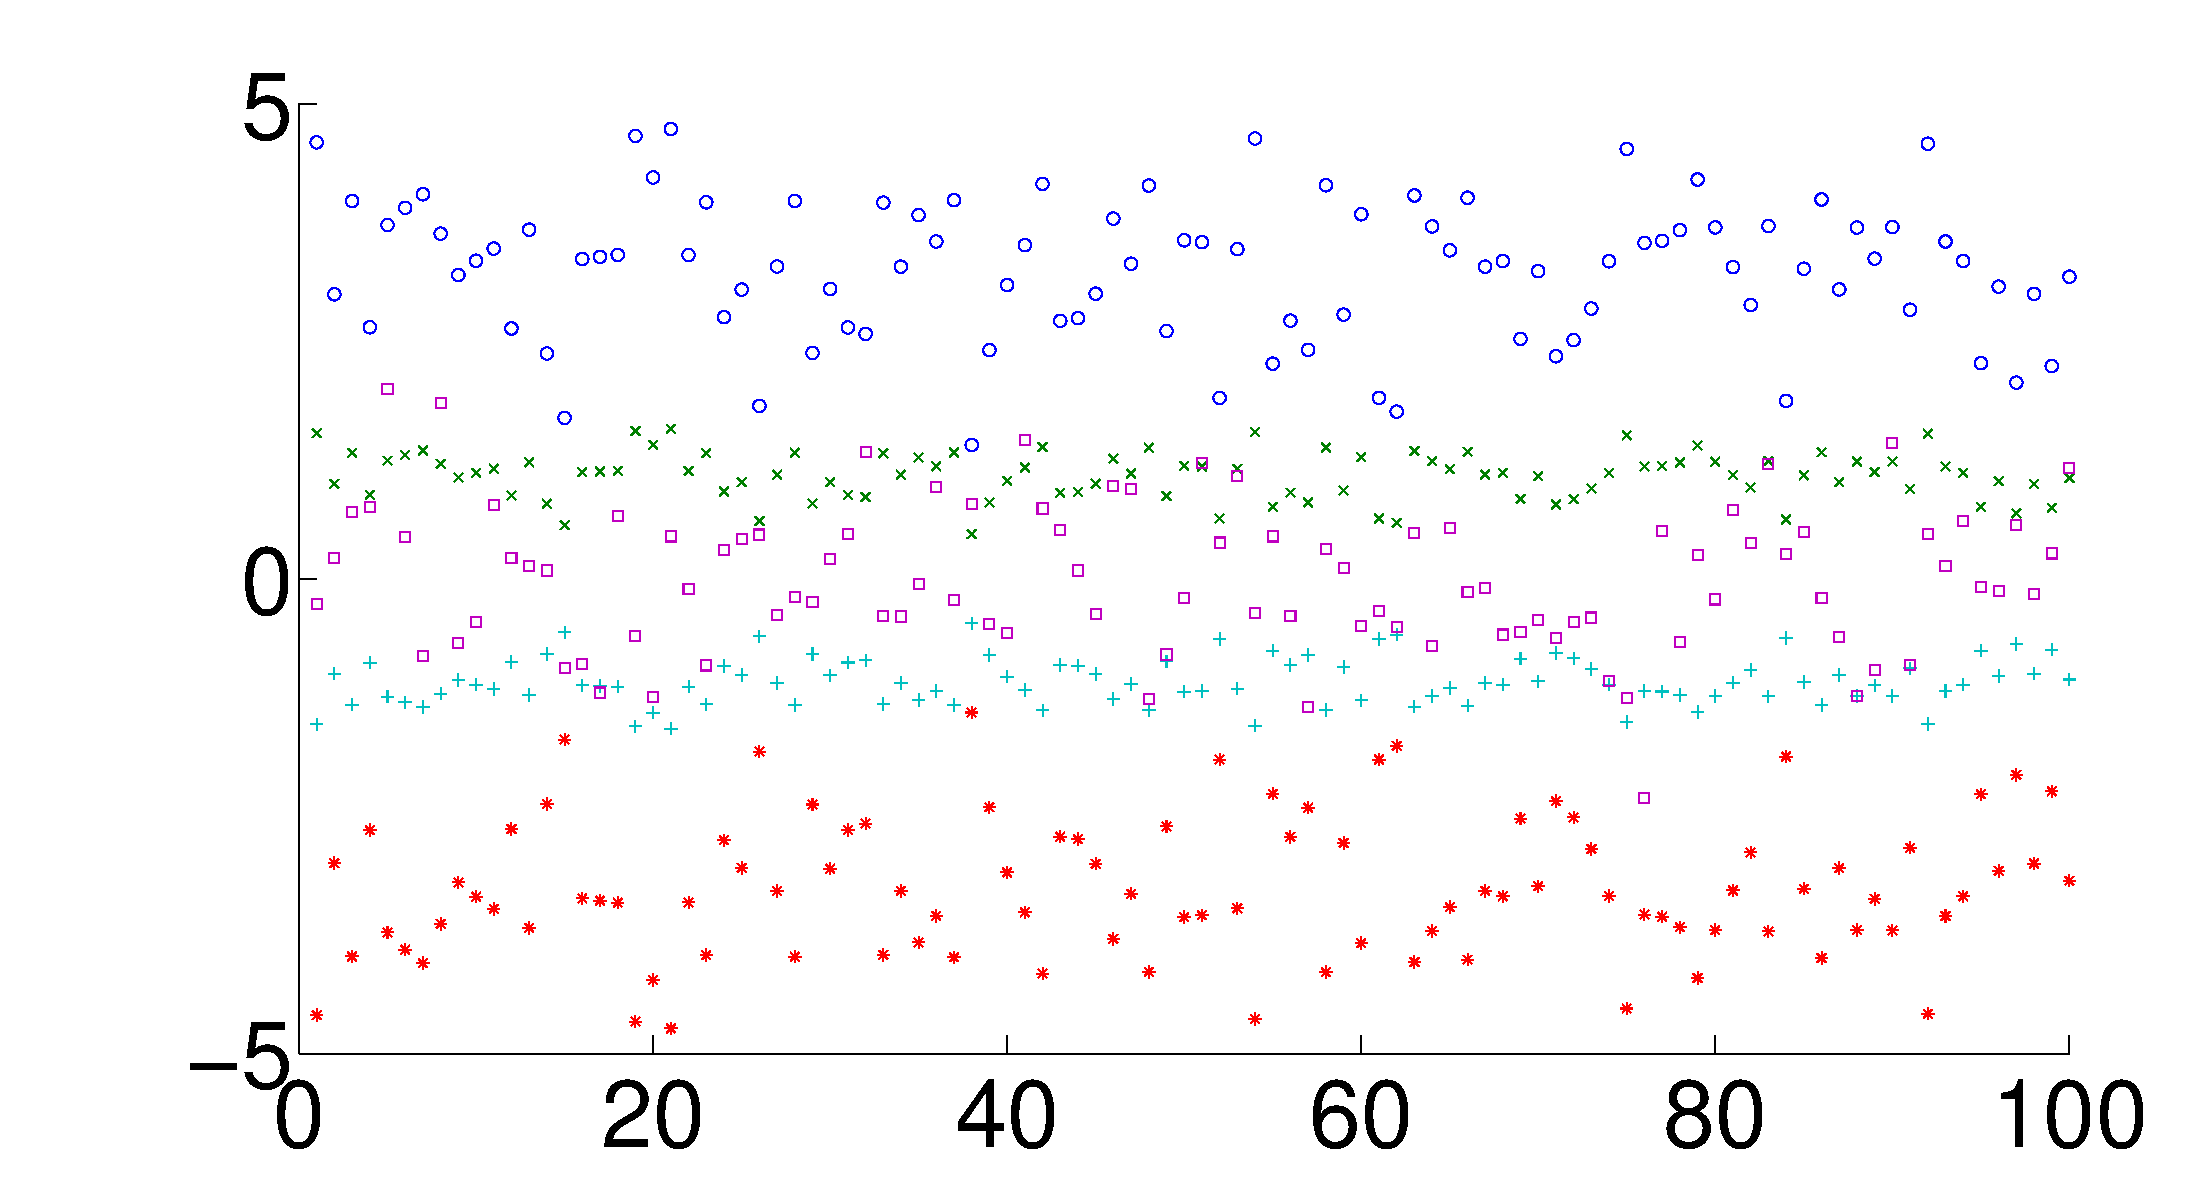
\includegraphics[scale=0.14]{fig/clusters.eps} &
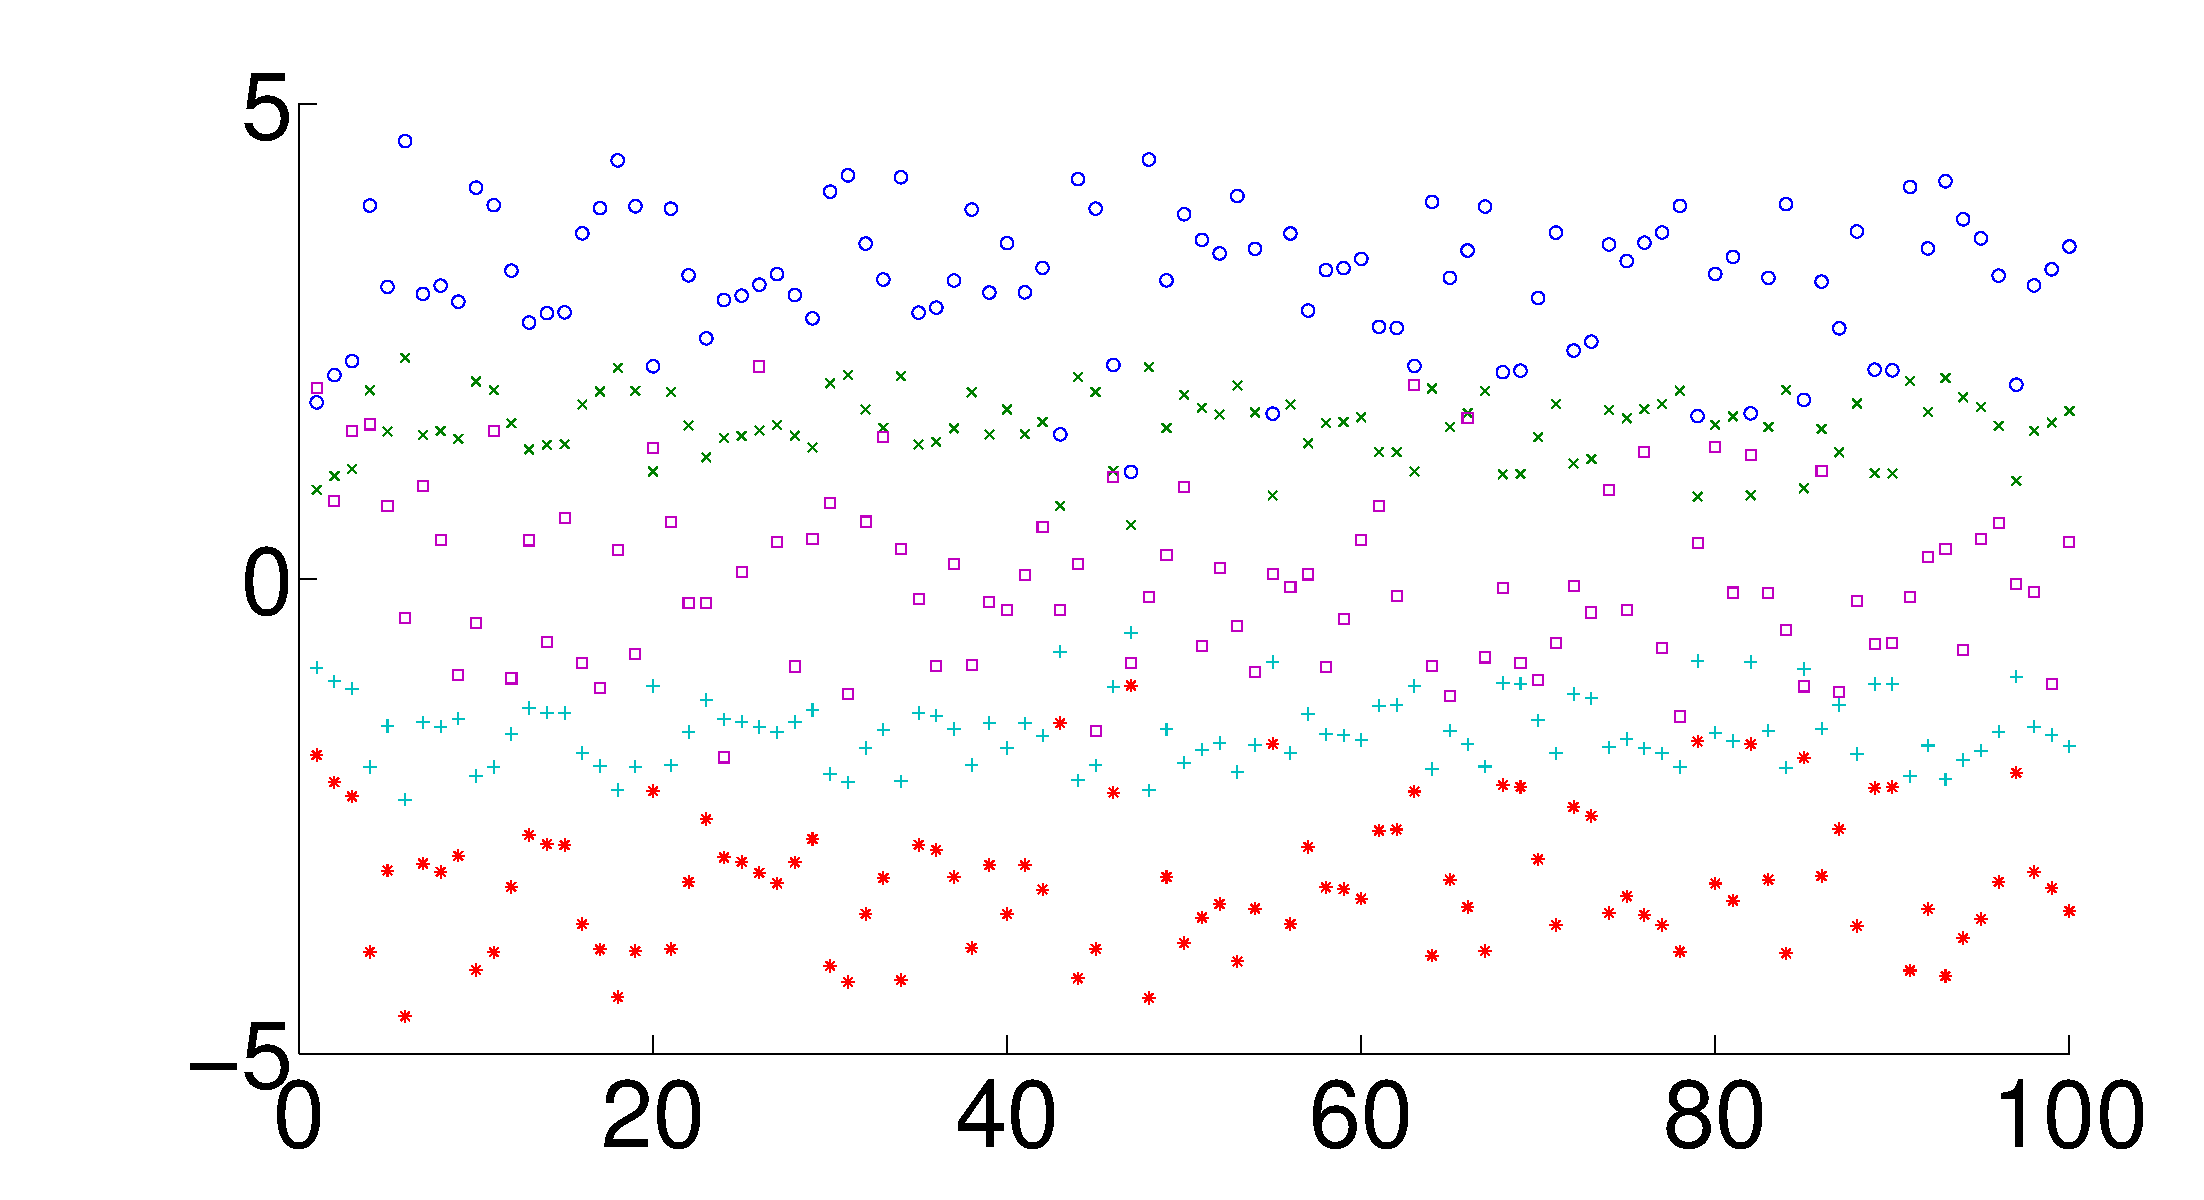
\includegraphics[scale=0.14]{fig/clusters4.eps} &
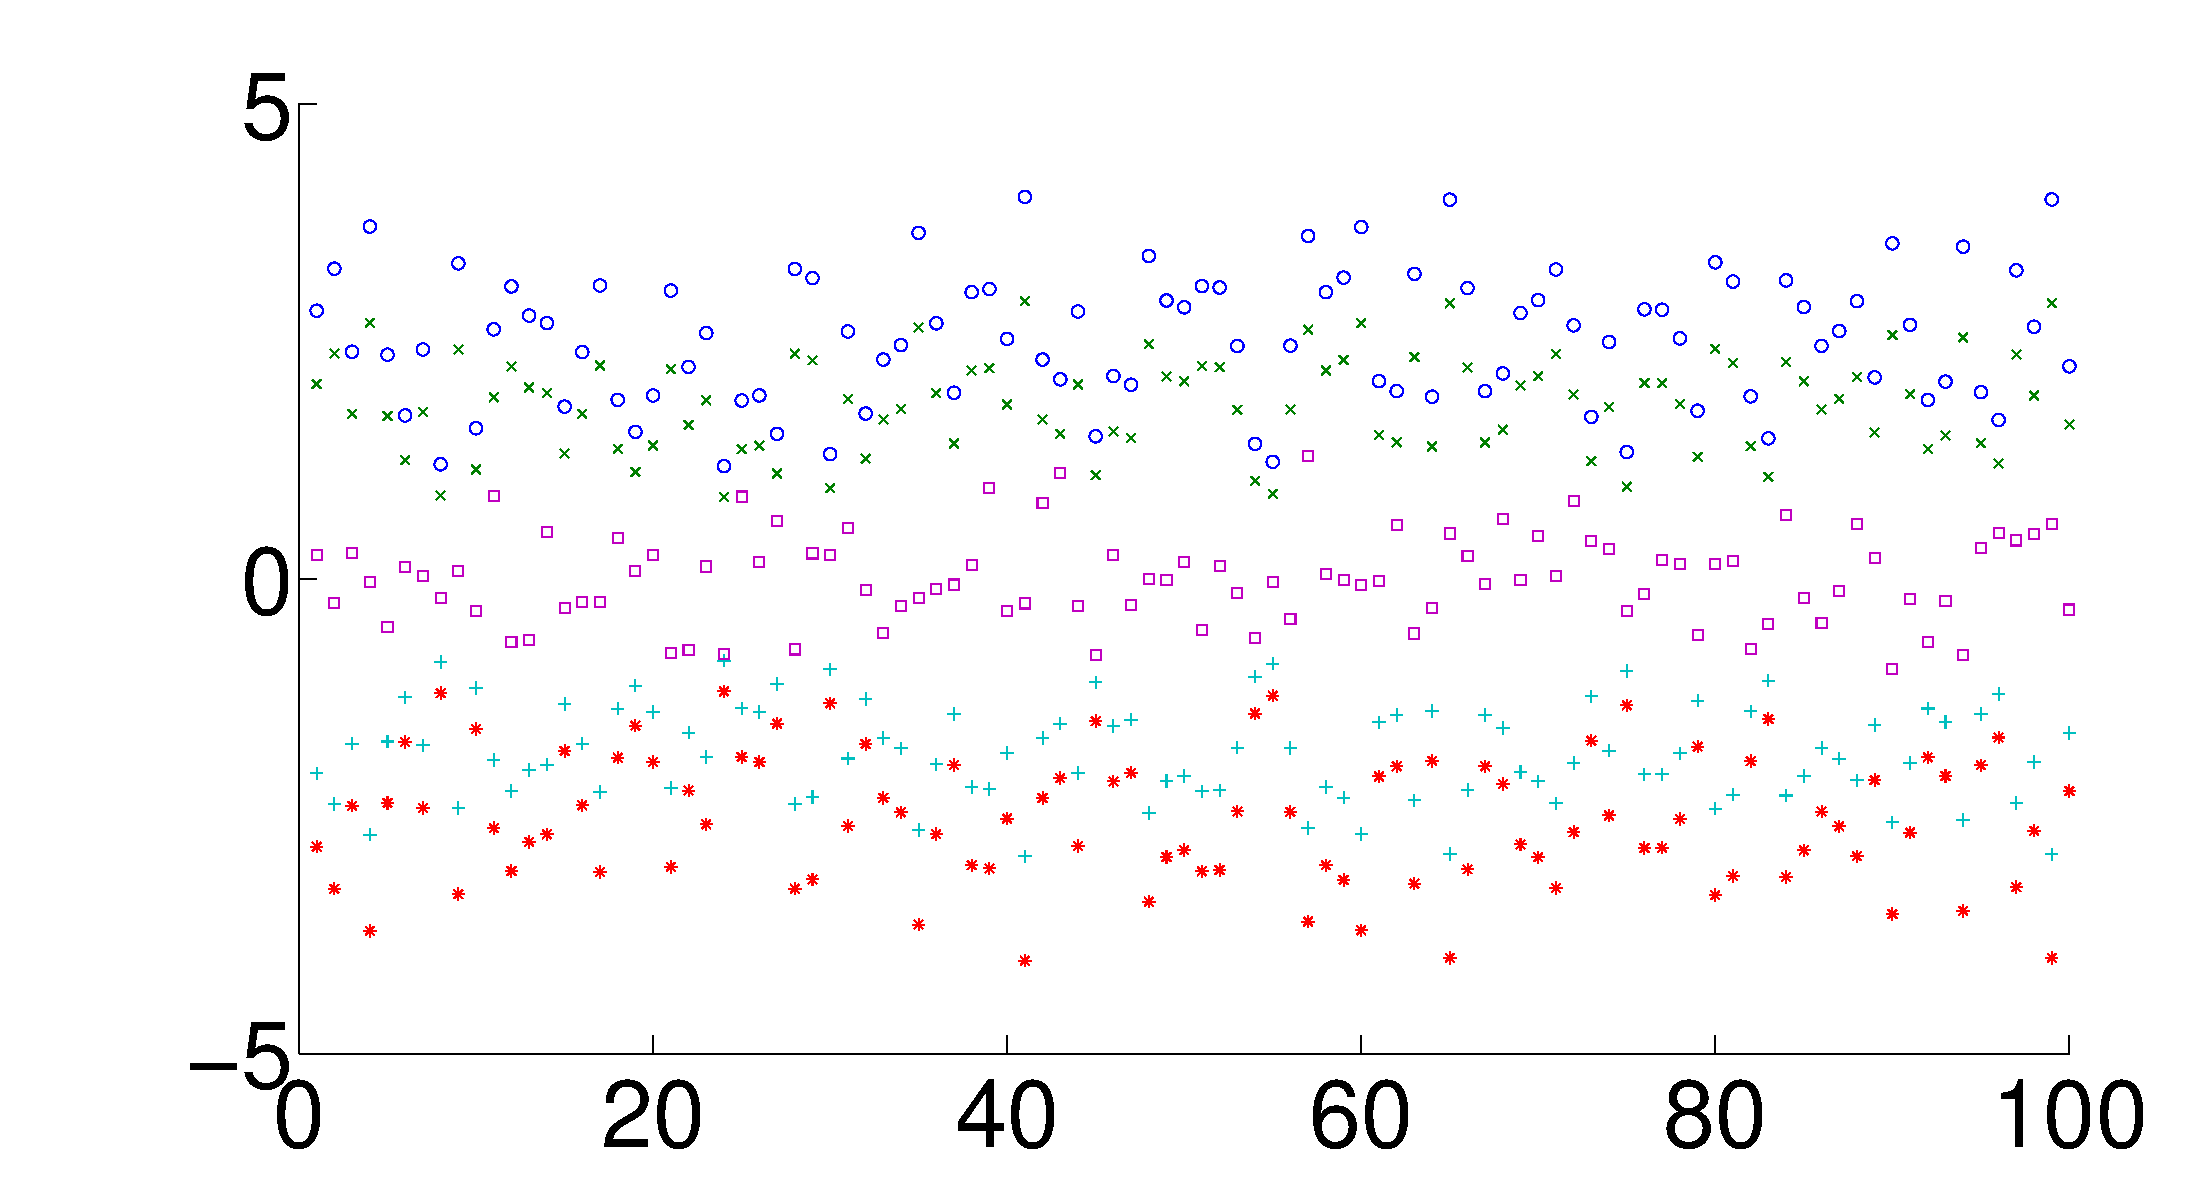
\includegraphics[scale=0.14]{fig/clusters3.eps} \\
$a_1$ --- range: [-4.74, 4.74] & $a_3$ --- range: [-4.61, 4.61] & $a_2$ --- range: [-4.02, 4.02] \\
$\mu$: 0, $\sigma$:2.26 &$\mu$: 0, $\sigma$:2.30 & $\mu$: 0, $\sigma$:2.18 \\
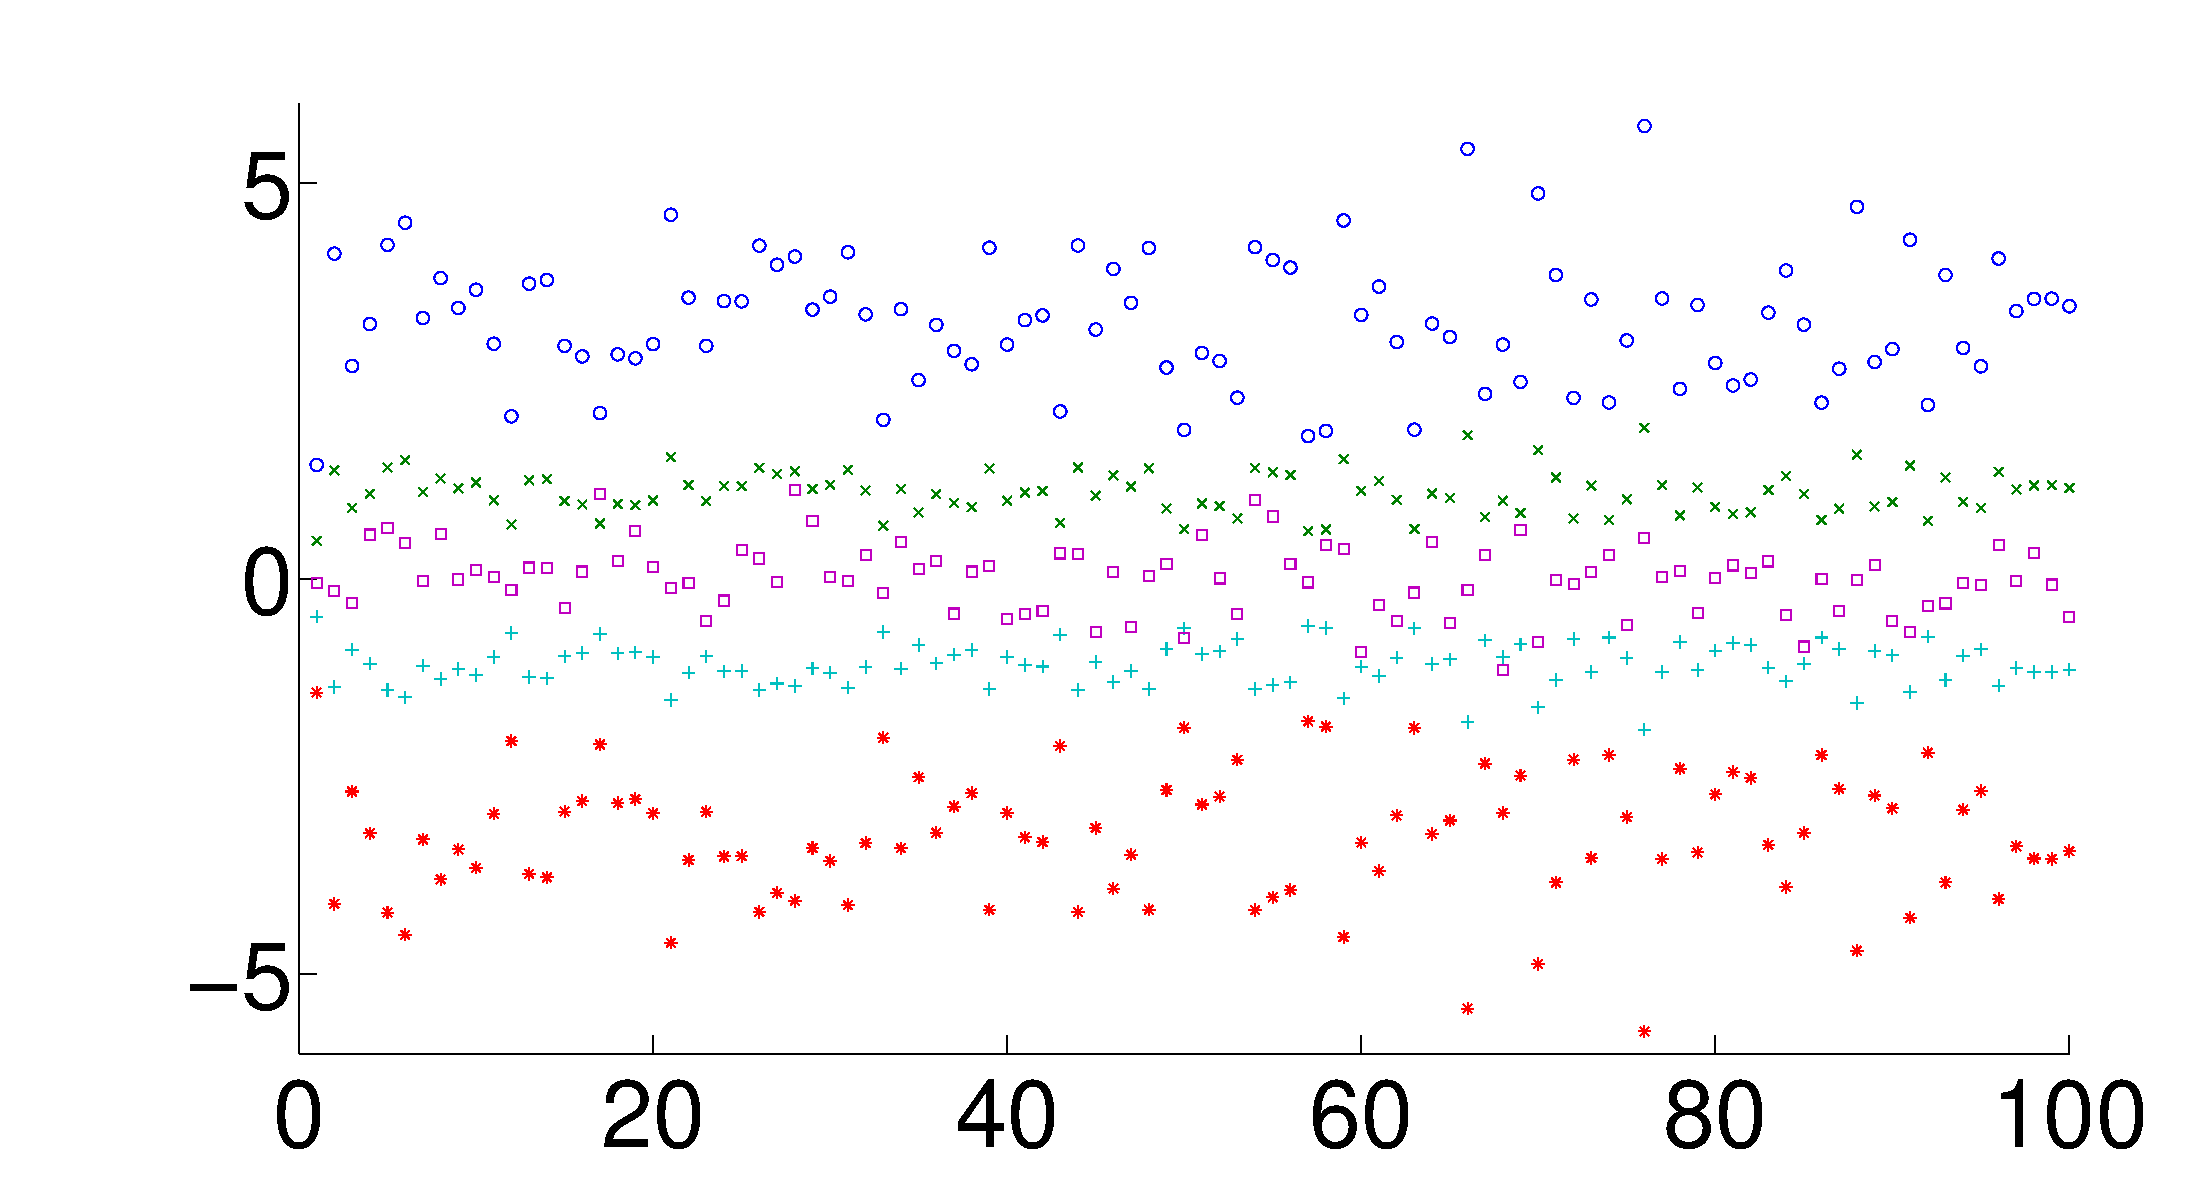
\includegraphics[scale=0.14]{fig/clusters21.eps} &
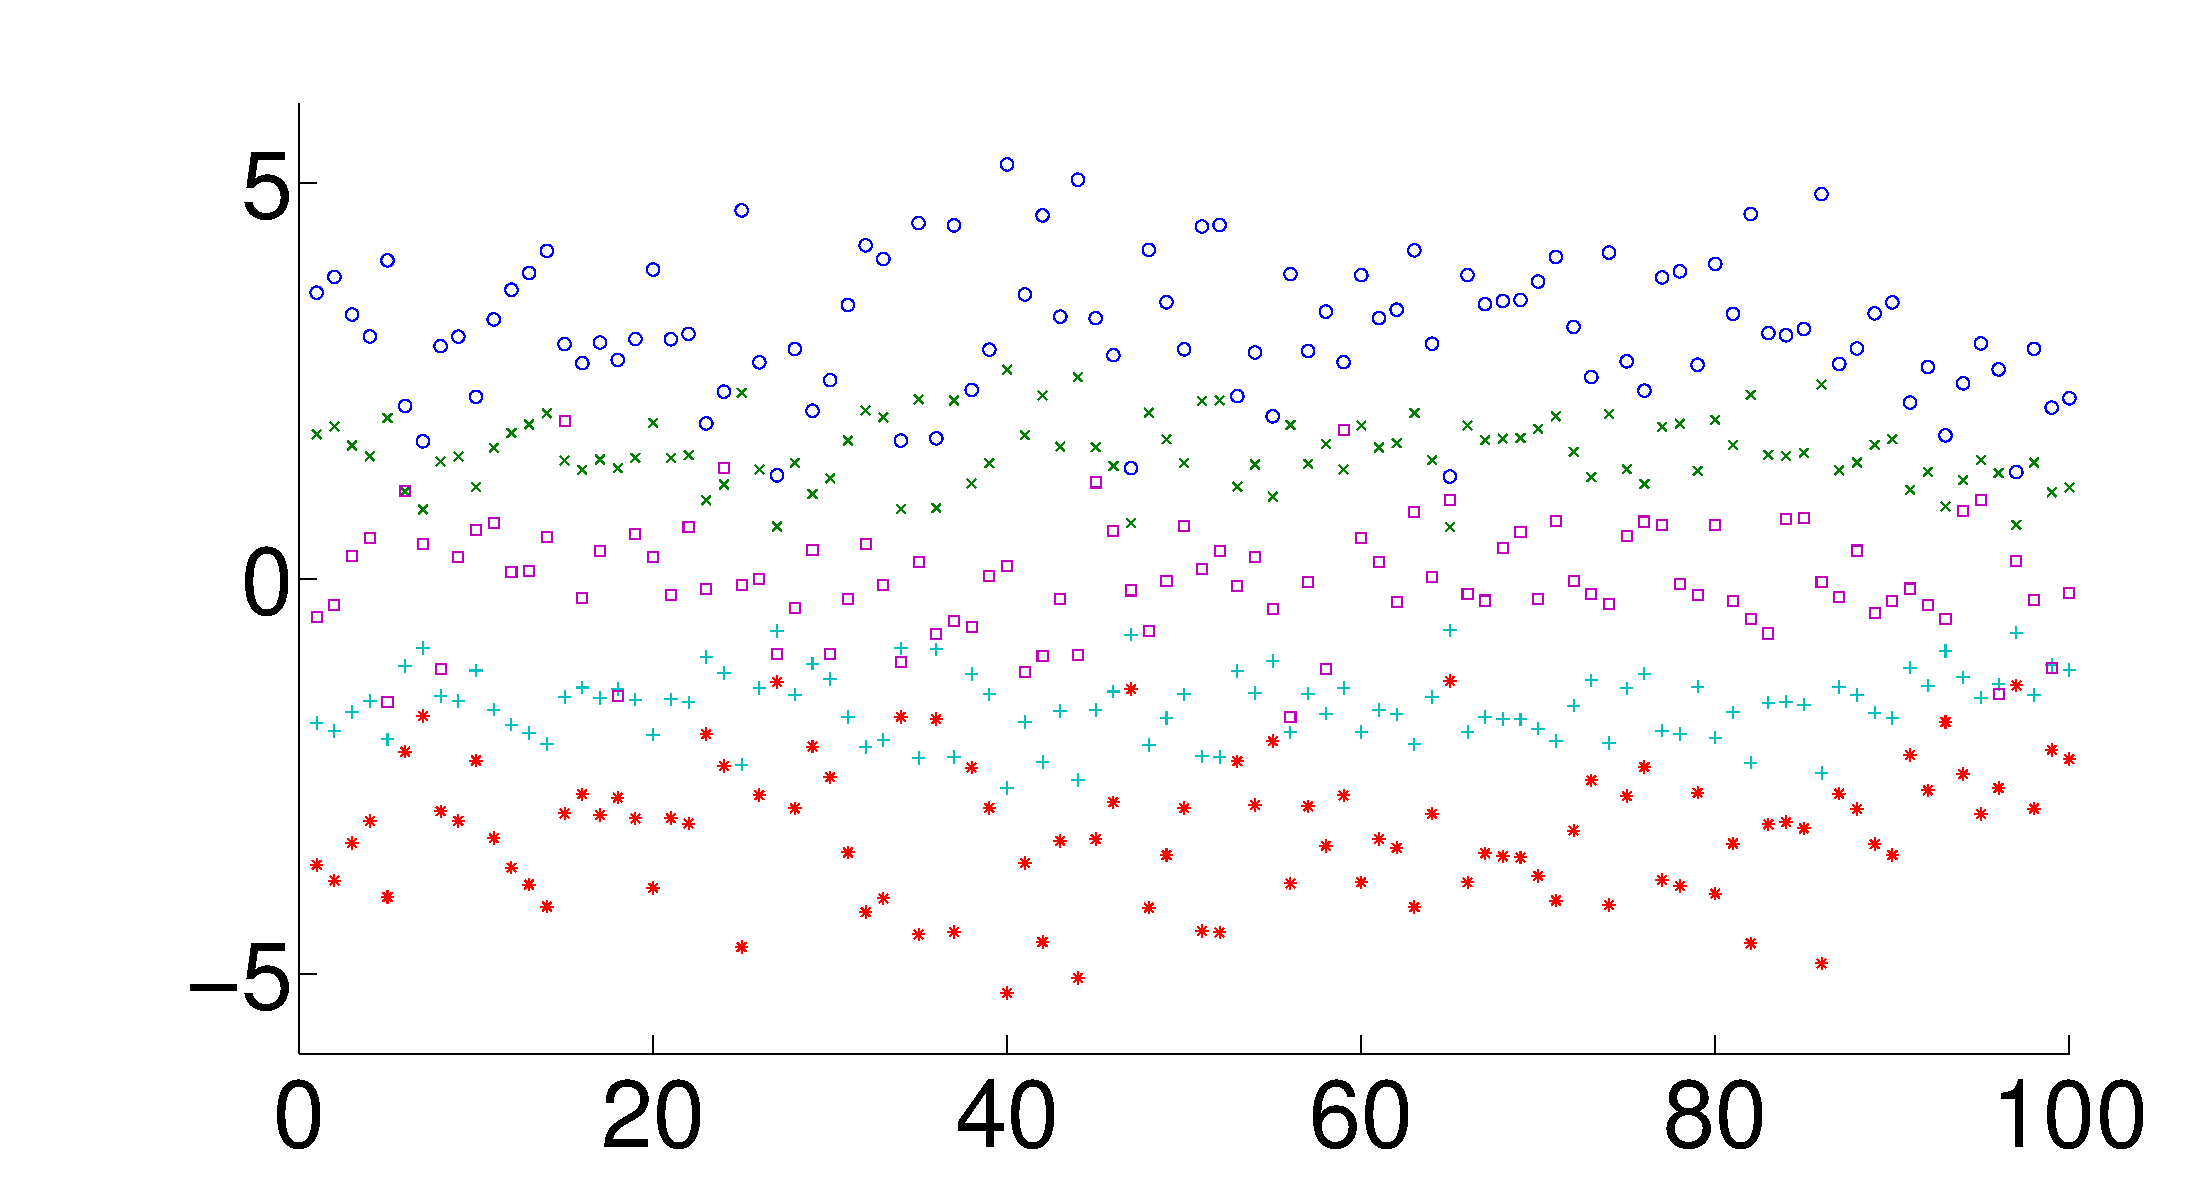
\includegraphics[scale=0.14]{fig/clusters23.eps} &
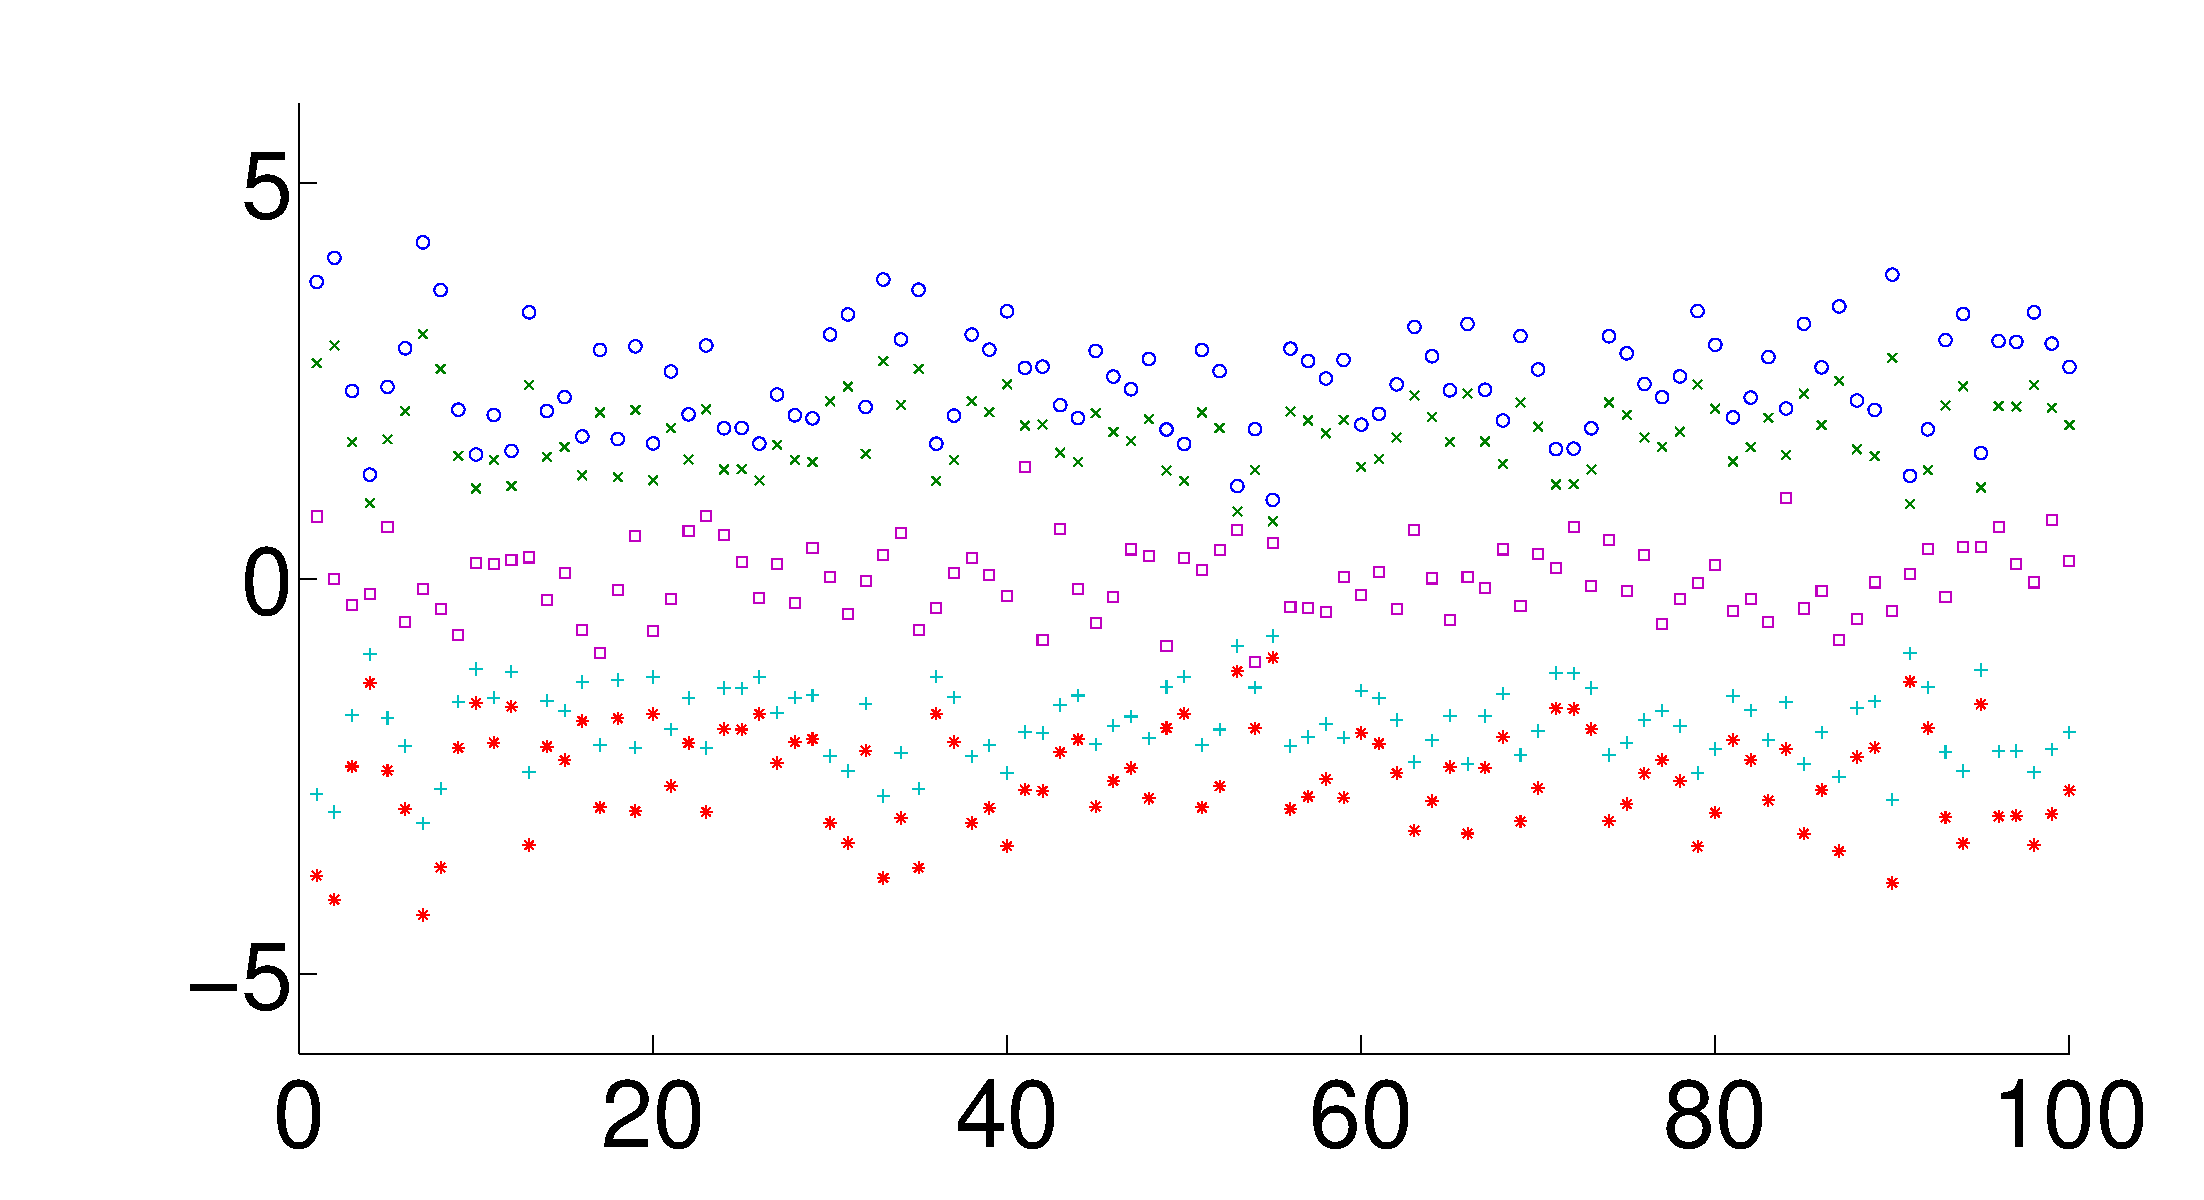
\includegraphics[scale=0.14]{fig/clusters22.eps} \\
$a_1'$ --- range: [-5.72, 5.72] & $a_3'$ --- range: [-5.24, 5.24] & $a_2'$ --- range: [-4.25, 4.25] \\
$\mu$: 0, $\sigma$:2.20 & $\mu$: 0, $\sigma$:2.35 & $\mu$: 0, $\sigma$:2.15 \\
\end{tabular}
\end{center}
\caption{\label{fig:syndata} Scatter plots of data instances from three sample attributes in one synthetic dataset (upper frame) and those of their corresponding attributes from another (lower frame) are illustrated to show their respective value distributions.}
\end{figure*}

\subsubsection{Results:}
Figure~\ref{fig:syn_pareto} illustrates the Pareto front obtained from matching two synthetic datasets, each having 20 attributes and 5 clusters. Most notably, the gold standard results for both attribute matching and cluster matching are obtained from the left-most point on the Pareto front. In other words, given the decision variables ($X$) corresponding to that point, we obtained 100\% correct matching results. We further observed that in our subsequent tests on other synthetic datasets with varied number of attributes and clusters, the derived Pareto fronts all contain gold standard result, and the point corresponding to the gold standard can always be found towards the minimum end of $f_a$. Given this, we propose the following method to reduce the Pareto-optimal set to a single point corresponding to the most favored choice ($X^*$) in the decision space. The idea is to find the decision with the minimum weighted sum of objective values in the obtained Pareto-optimal set, i.e., $X^*=\stackbin[X]{}{\argmin}~\big[\alpha f_a(X)+\beta f_c(X)\big]$, where $\alpha$ and $\beta$ are weights. We first conducted preliminary experiments to determine the best values for $\alpha$ and $\beta$ (0.8 and 0.2 respectively) and used them in all subsequent experiments. This method works markedly well on the synthetic datasets. For all the tests described in Table~\ref{tbl:scale}, 100\% correct results for both attribute and cluster matchings are obtained (hence we omit the precision in the table).
\begin{figure}[tb]
\begin{center}
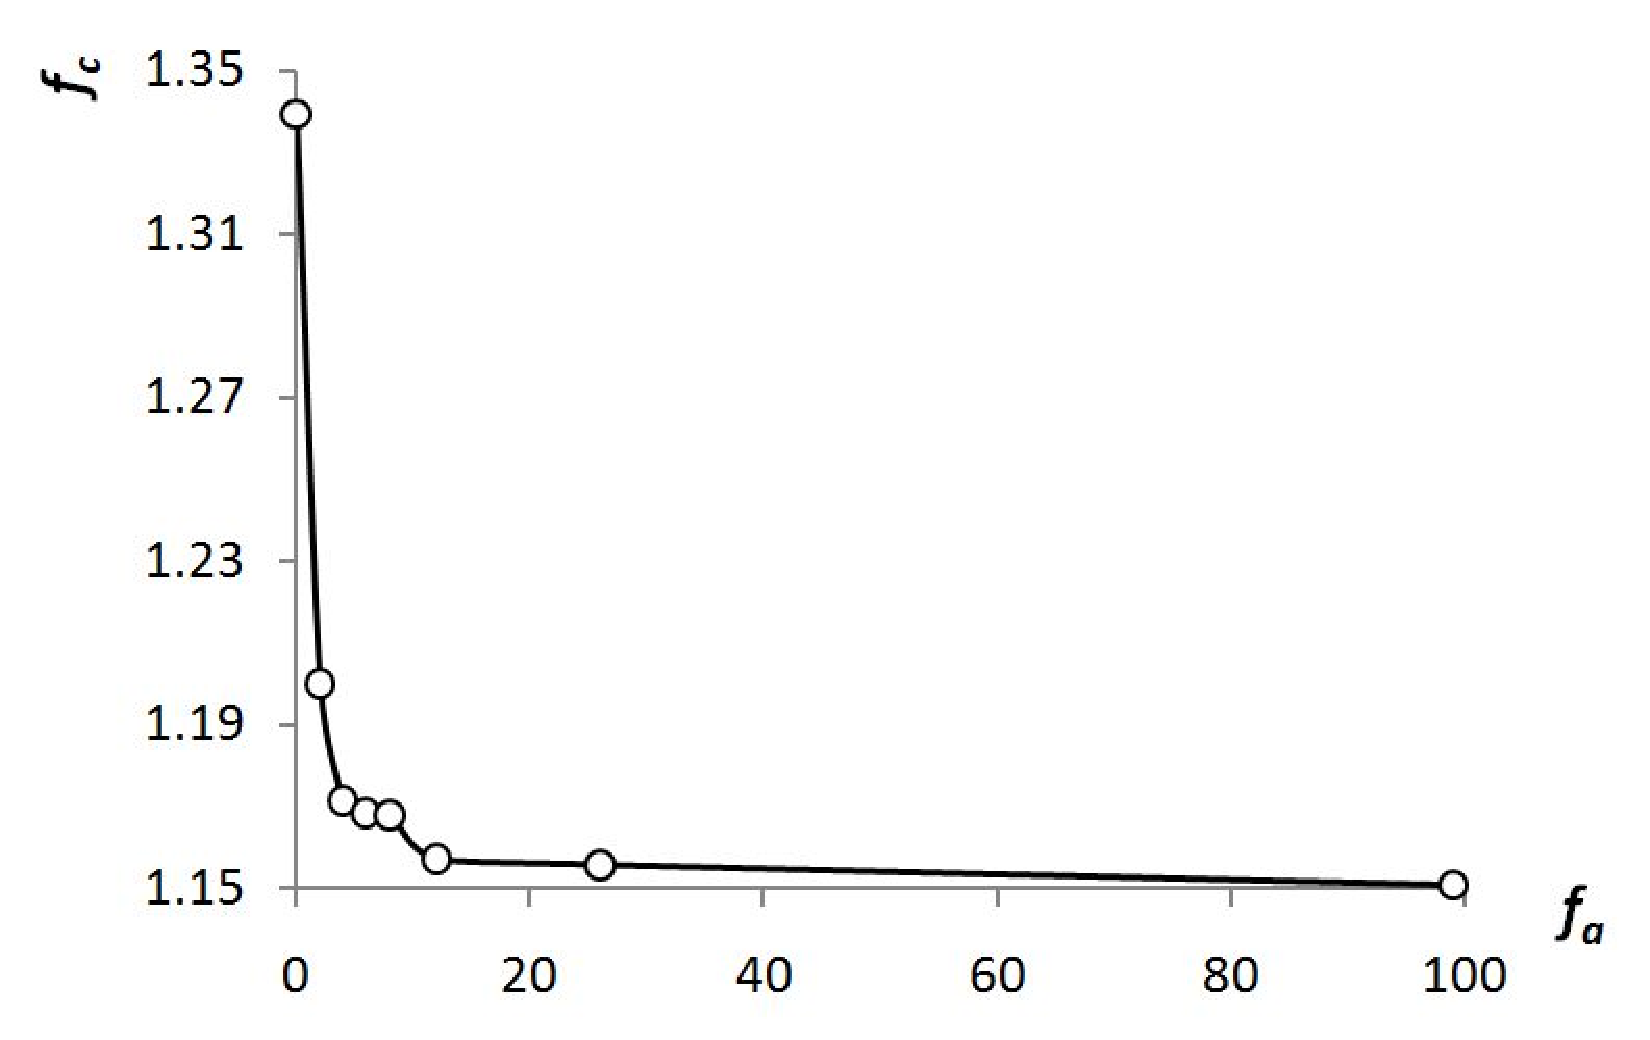
\includegraphics[width=0.6\textwidth]{fig/syn_pareto.eps}
\end{center}
\caption{\label{fig:syn_pareto} An example Pareto front obtained from matching two synthetic datasets with 20 attributes and 5 clusters.}
\end{figure}

\subsubsection{Running Time:}
We systematically altered the number of attributes and clusters present in the data and conducted a series of tests to show the scalability of the proposed method. The running time under different configurations is reported in Table~\ref{tbl:scale}. The time is calculated by averaging over 5 runs of each test (on a 2.53GHz dual-core CPU with 4 gigabytes memory), each run having 1000 iterations in the simulated annealing process. The main computationally expensive part of the annealing process is the generation of new candidate solution phase (function $G$) in which an assignment problem is solved using the Hungarian method. The complexity of the Hungarian method is cubic and is already the most efficient algorithm for solving the assignment problem (a brute force algorithm has a factorial complexity). Fortunately, rarely is the case that the number of attributes or clusters is large in real-world scenarios where the proposed technique is needed. For reasonable configurations in most practical applications, the computation time is within a tractable range as shown in table~\ref{tbl:scale}.
\begin{table}[tbh]
\begin{center}
\begin{tabular}{r|r|r}
\hline
\# attributes & \# clusters & time (sec)\\
\hline
5   &   20  &   0.28\\
20  &   20  &   1.81\\
20  &   40  &   7.04\\
20  &   60  &   17.80\\
40  &   20  &   4.66\\
40  &   40  &   11.74\\
40  &   60  &   25.93\\
60  &   20  &   10.95\\
60  &   40  &   20.70\\
60  &   60  &   37.35\\
100 &   100 &   172.23\\
\hline
\end{tabular}
\end{center}
\caption{\label{tbl:scale} Running time of the annealing process on synthetic datasets with varied configurations of attribute and cluster sizes. The time is obtained by averaging over results of 5 runs of each test.}
\end{table}

\subsection{Neuroscience Dataset}
\subsubsection{Data Acquisition:}
%The difficulty is especially pronounced in many scientific domains where there have been an increasing interest in nationwide and worldwide inter-institute collaboration. An example of such collaborative project is research in experimental event-related brain potential (ERP) analysis carried out at the NEMO (Neural Electromagnetic Ontologies) consortium laboratories. The heterogeneity among participating groups hinders meaningful meta-analysis despite the large number of studies in the field.

To address the problems of attribute and cluster matching in a real-world neuroscience application, we used a set of realistic simulated ERP (event-related potentials) datasets, which were designed to support evaluation of ERP analysis methods~\cite{FrishkoffEtal07}. The datasets were specifically designed to simulate heterogeneous data from different groups of subjects under different conditions (via distinct simulated brain activities), as well as distinct measurement methods (spatial and temporal metrics) and distinct patterns (reflecting two different pattern decomposition techniques). Real ERP data arise from superposition of latent scalp-surface electrophysiological patterns, each reflecting the activity of a distinct cortical network that cannot be reconstructed from the scalp-measured data with any certainty. Thus, real ERP data are not appropriate for evaluation of ERP pattern mapping. By contrast, simulated ERP data are derived from known source patterns and therefore provide the necessary gold standard for evaluation of our proposed methods.

The raw data for this study consist of 80 simulated event-related potentials (ERPs), in which each ERP comprises simulated measurement data for a particular subject ($n$ = 40). The 40 simulated subjects are randomly divided into two 20-subject groups, SG1 and SG2, each containing 40 ERPs (20 subjects in 2 experimental conditions). Each ERP consists of a superposition of 5 latent varying spatiotemporal patterns. These patterns were extracted from the two datasets, SG1 and SG2, using two techniques: temporal Principal Components Analysis (tPCA) and spatial Independent Components Analysis (sICA), two data decomposition techniques widely used in ERP research~\cite{Dien2010}. To quantify the spatiotemporal characteristics of the extracted patterns, two alternative metric sets, m1 and m2, were applied to the two tPCA and the two sICA derived datasets. For a complete explanation of these alternative metrics, please see Appendix in~\cite{FrishkoffEtal07}.

In summary, the simulated ERP data generation process yielded eight test datasets in total, reflecting a 2 (attribute sets) $\times$ 2 (subject groups) $\times$ 2 (decomposition methods) factorial design. Therefore, for each attribute sets there are 4 datasets generated from different combinations of subject groups and decomposition methods, resulting $4 \times 4 = 16$ cases for the studies of attribute matching and cluster matching. The reason to include such variabilities was to test the robustness of our matching method to different sources of heterogeneity across the different datasets. Within all test datasets, 5 major ERP spatiotemporal patterns are present. They are P100, N100, N3, MFN, and P300. These patterns can be identified in the datasets by clustering analysis. Pretending that the latent patterns underlying discovered clusters are unknown, we hope to match clusters across datasets to recover the fact that the same patterns are present in all datasets.

\subsubsection{Results:}
%Figure~\ref{fig:nemo_exp} illustrates the Pareto fronts derived by the proposed method on each of the 16 test cases.
We applied the weighted sum method as the post-process step after obtaining the Pareto-optimal solutions to determine the most favored choice using the parameters ($\alpha$ and $\beta$) discovered in the preliminary experiments on synthetic datasets (cf. Section~\ref{sec:syn_exp}). The accuracy of attribute matching and cluster matching along with the number of points in the Pareto front are listed in Table~\ref{tbl:nemo_perf} (all these results are obtained by taking average from 5 runs for each test case).

%\begin{figure*}[tb]
%\begin{center}
%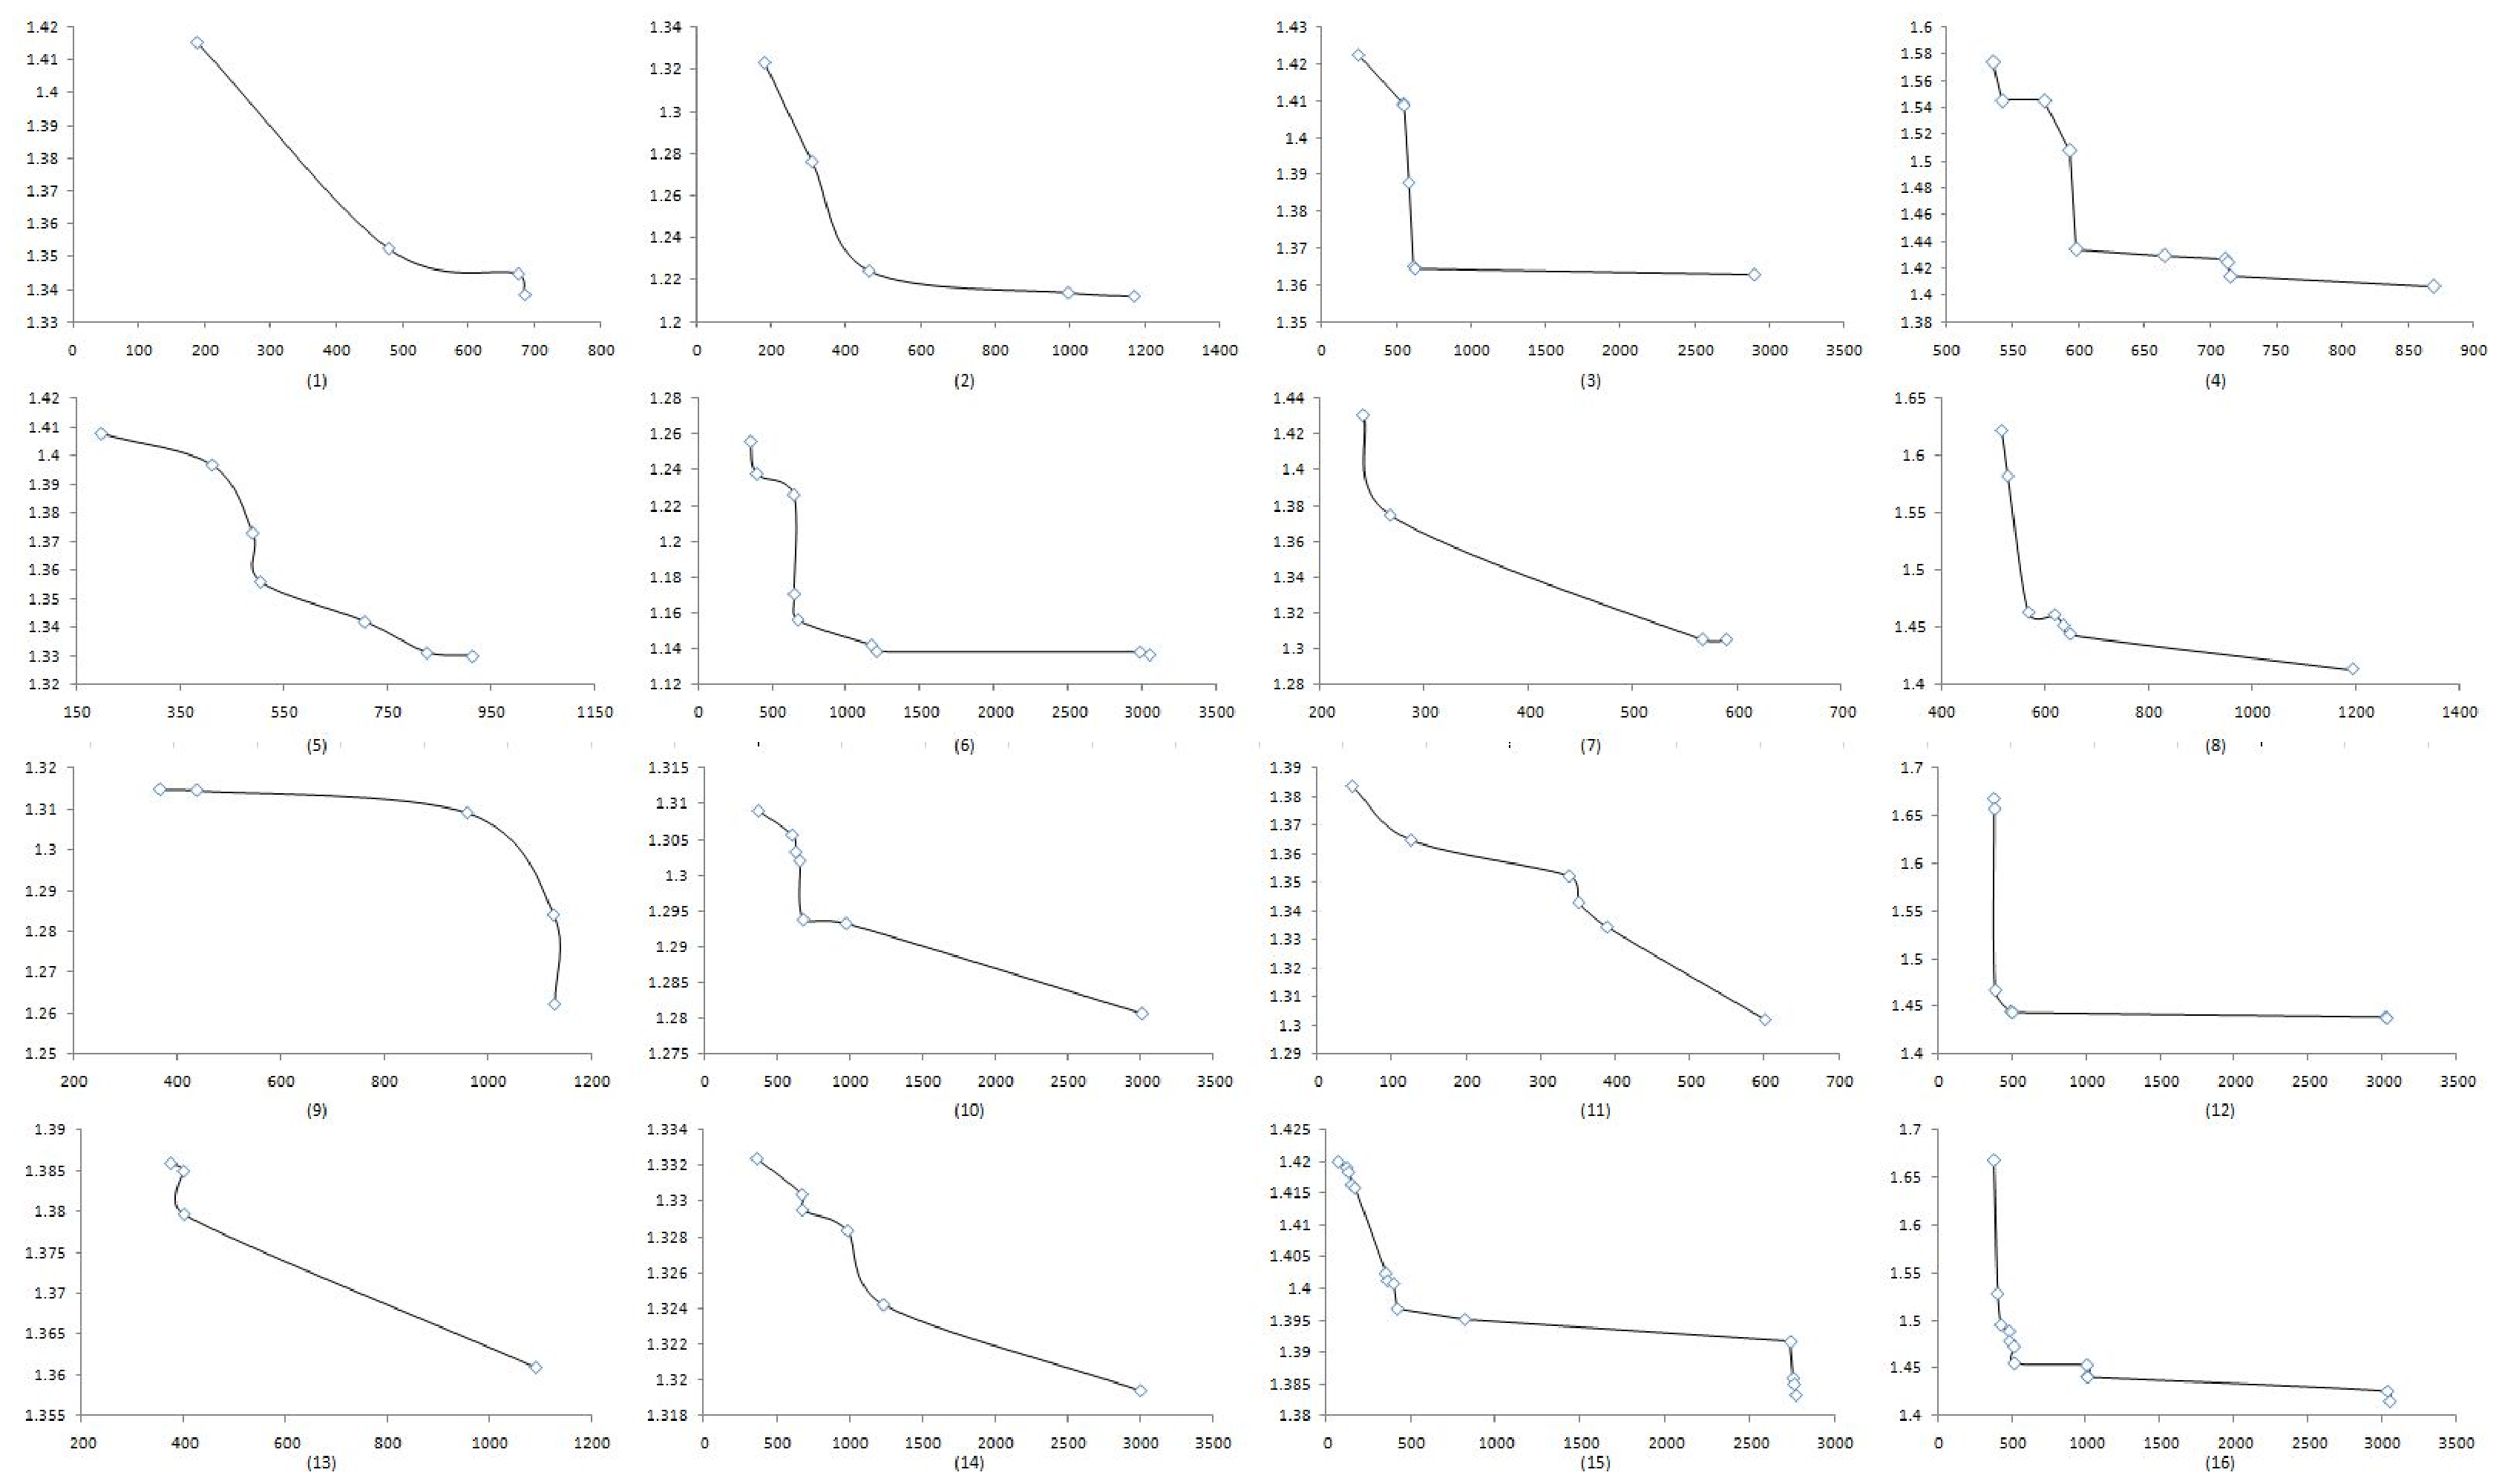
\includegraphics[width=1.\textwidth]{nemo_exp2.eps}
%\end{center}
%\caption{\label{fig:nemo_exp} Pareto fronts obtained from the 16 test cases of the neuroscience dataset.}
%\end{figure*}

It can be observed from the results in Table~\ref{tbl:nemo_perf} that more different factors involved in the acquisition of the two datasets for matching can negatively affect the matching performance. For example, in test case 1, the two datasets are drawn from the same subject group (SG1) and preprocessed using the same decomposition method (sICA); whereas in test case 4, the subject groups and decomposition methods are all different, resulting in greater variability and hence the performance is less satisfactory. However, it is worth noting that our method greatly outperforms traditional whole-attribute-based statistic characterization, as is shown in Figure~\ref{fig:perf_comp}. In this figure we also demonstrate the accuracy of the segmented statistics characterization with expert-labeled patterns, meaning that the data is partitioned and aligned in the most accurate way, which marks the best achievable attribute matching performance. But it is not feasible because, as mentioned in~Section~\ref{sec:intro}, manually recognizing patterns (partitioning data) and aligning them across datasets requires a priori knowledge of attributes in the datasets which is exactly what the problem of attribute matching tries to discover (the circular causality problem). On the other hand, our method does not require human involvement (except the specification of the number of clusters (patterns) present in the data in order to run the clustering analysis) in determining both the attribute matching and cluster matching and is able to achieve close-to-optimal results.

\begin{figure*}[tb]
\begin{center}
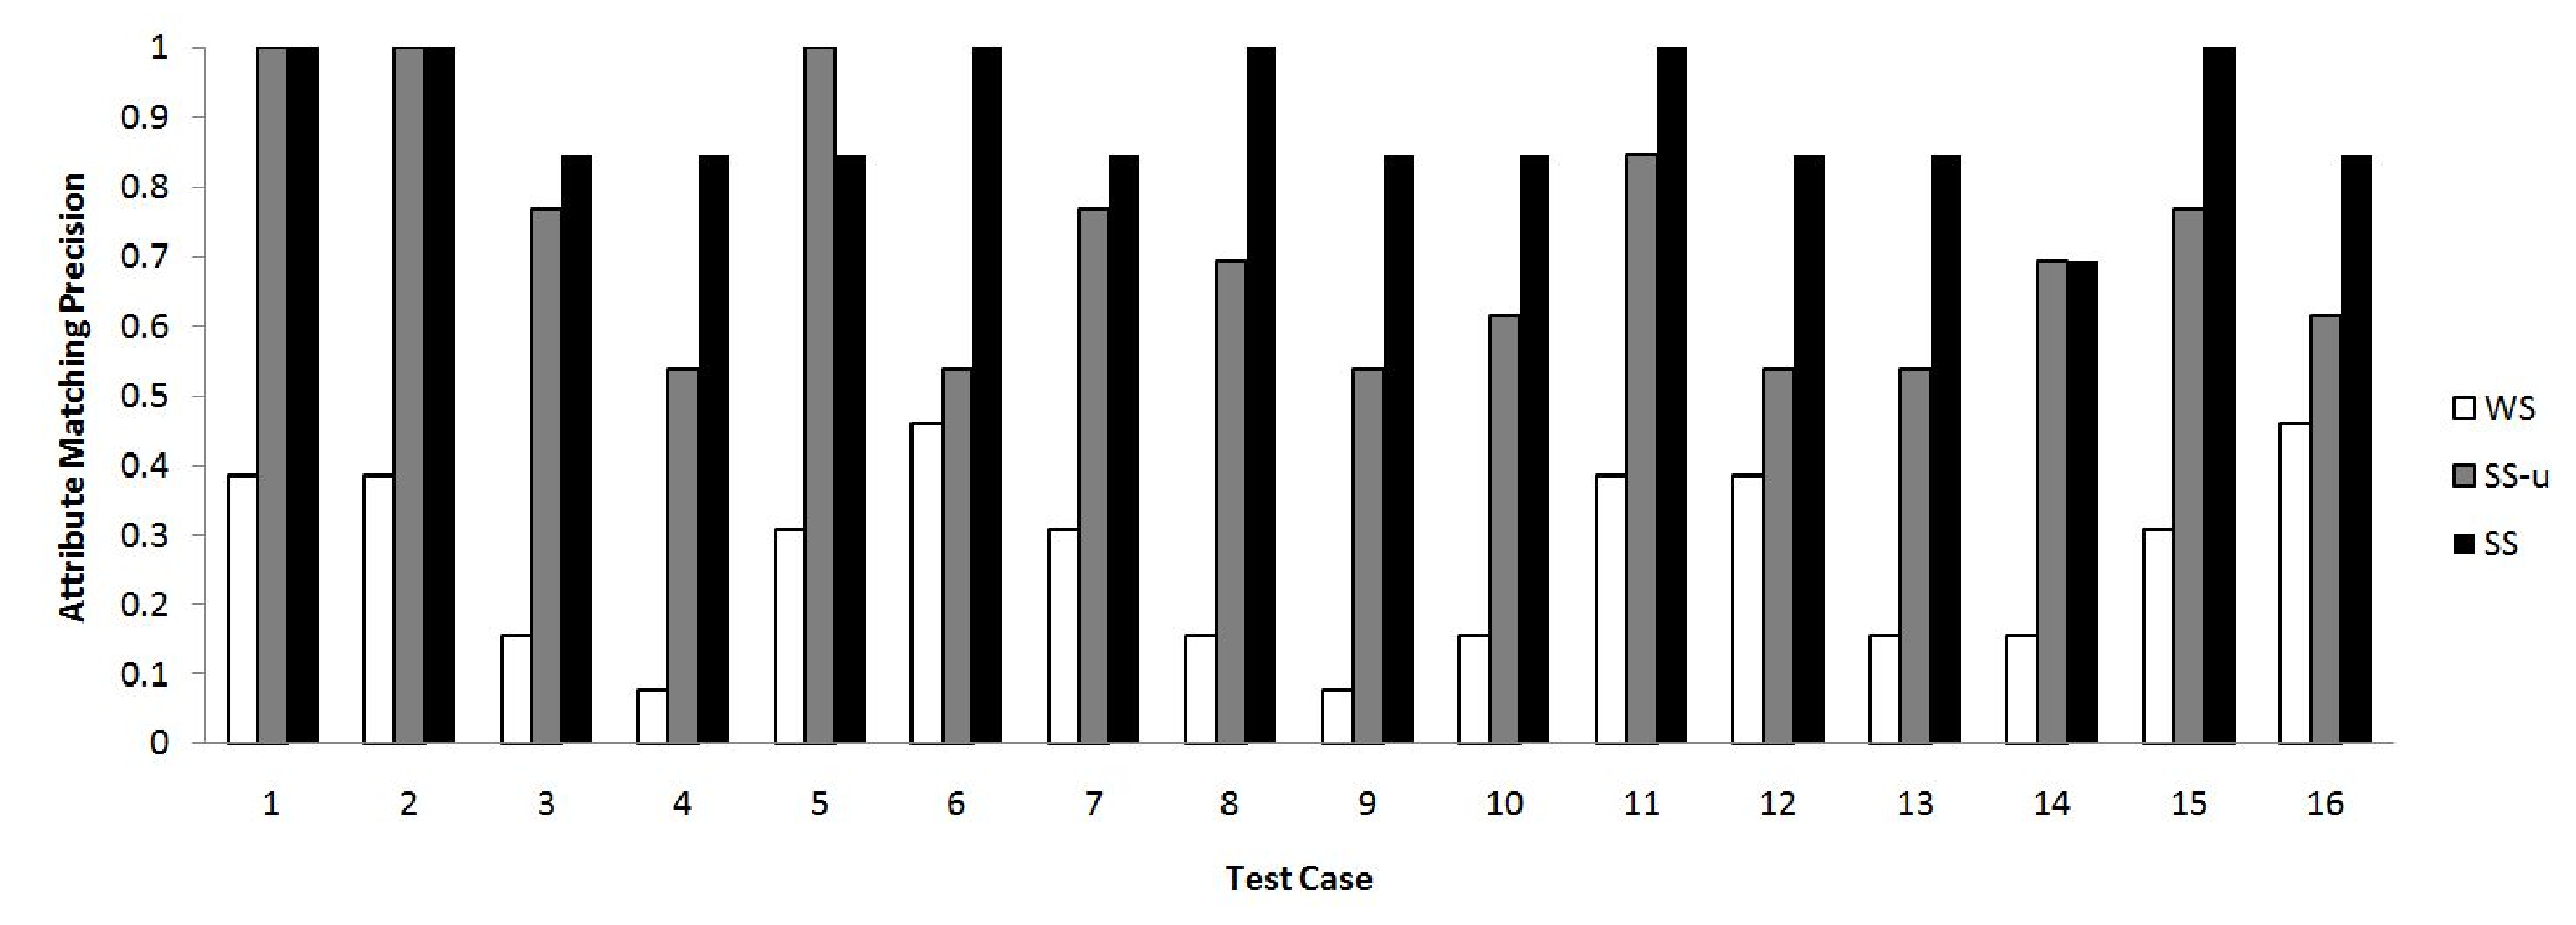
\includegraphics[width=1.\textwidth]{fig/perf_comp.eps}
\end{center}
\caption{\label{fig:perf_comp} A comparison of the attribute matching accuracy of three methods on the 16 test cases of the neuroscience dataset. The three methods being compared are matching based on whole-attribute statistics (WS), segmented attribute statistics without knowing a priori cluster matching (SS-u), and segmented attribute statistics with expert-aligned clusterings (SS).}
\end{figure*}


\begin{table*}[tbh]
\begin{center}
\begin{tabular}{l|l|l|l|l|l}
\hline
Test case & Source params & Target params & $~~~P_a~~~$ & $~~~P_c~~~$ & $|\Sigma|$\\
\hline
1		&	$\langle$	SG1, sICA, m1	$\rangle$	&	$\langle$	SG1, sICA, m2	$\rangle$	&		13/13	&	5/5	&	5	 \\
2		&	$\langle$	SG1, sICA, m1	$\rangle$	&	$\langle$	SG2, sICA, m2	$\rangle$	&		13/13	&	5/5	&	6	 \\
3		&	$\langle$	SG1, sICA, m1	$\rangle$	&	$\langle$	SG1, tPCA, m2	$\rangle$	&		10/13	&	5/5	&	6	 \\
4		&	$\langle$	SG1, sICA, m1	$\rangle$	&	$\langle$	SG2, tPCA, m2	$\rangle$	&		7/13	&	3/5	&	8	 \\
5		&	$\langle$	SG2, sICA, m1	$\rangle$	&	$\langle$	SG1, sICA, m2	$\rangle$	&		11/13	&	3/5	&	7	 \\
6		&	$\langle$	SG2, sICA, m1	$\rangle$	&	$\langle$	SG2, sICA, m2	$\rangle$	&		13/13	&	5/5	&	7	 \\
7		&	$\langle$	SG2, sICA, m1	$\rangle$	&	$\langle$	SG1, tPCA, m2	$\rangle$	&		10/13	&	5/5	&	6	 \\
8		&	$\langle$	SG2, sICA, m1	$\rangle$	&	$\langle$	SG2, tPCA, m2	$\rangle$	&		9/13	&	2/5	&	8	 \\
9		&	$\langle$	SG1, tPCA, m1	$\rangle$	&	$\langle$	SG1, sICA, m2	$\rangle$	&		7/13	&	5/5	&	4	 \\
10		&	$\langle$	SG1, tPCA, m1	$\rangle$	&	$\langle$	SG2, sICA, m2	$\rangle$	&		8/13	&	5/5	&	6	 \\
11		&	$\langle$	SG1, tPCA, m1	$\rangle$	&	$\langle$	SG1, tPCA, m2	$\rangle$	&		11/13	&	5/5	&	6	 \\
12		&	$\langle$	SG1, tPCA, m1	$\rangle$	&	$\langle$	SG2, tPCA, m2	$\rangle$	&		7/13	&	3/5	&	5	 \\
13		&	$\langle$	SG2, tPCA, m1	$\rangle$	&	$\langle$	SG1, sICA, m2	$\rangle$	&		7/13	&	3/5	&	5	 \\
14		&	$\langle$	SG2, tPCA, m1	$\rangle$	&	$\langle$	SG2, sICA, m2	$\rangle$	&		9/13	&	5/5	&	6	 \\
15		&	$\langle$	SG2, tPCA, m1	$\rangle$	&	$\langle$	SG1, tPCA, m2	$\rangle$	&		10/13	&	3/5	&	8	 \\
16		&	$\langle$	SG2, tPCA, m1	$\rangle$	&	$\langle$	SG2, tPCA, m2	$\rangle$	&		8/13	&	3/5	&	8	 \\
\hline
\end{tabular}
\end{center}
\caption{\label{tbl:nemo_perf} Matching performance of the proposed method with MOSA on the 16 test cases from the neuroscience dataset. The source and target parameter configuration of the data acquisition process of each test case are shown. $P_a$ and $P_c$ denote the accuracy of attribute matching and cluster matching respectively. $\Sigma$ is the number of points in the obtained Pareto-front. The quantities listed in the table are obtained by averaging over 5 runs of each test.}
\end{table*}

\subsection{Comparison with Multi-Objective Genetic Algorithm}
The concept of Genetic Algorithm (GA) was developed by Holland and his colleagues~\cite{Holland1992}. GA is first inspired by the evolutionary process in which weak and unfit species within their environment are faced with extinction and stronger ones have greater opportunities to pass their genes to next generation. Comparing to Simulated Annealing, Genetic Algorithm often offers a different perspective in the field of numerical optimization. Starts from a number of random generated population, cross over and evolve; GA has the ability to search in parallel around different and often fully scattered instances in the solution space, in contrast to the ``single thread" search in Simulated Annealing. In this paper, we also implemented the Multi-Objective Genetic Algorithm as the metaheuristics to solve the dual matching problem.

%For the crossover operation in our MOGA implementation, we go through all the attributes (clusters) in a random sequence, if the matching of one attribute in both parents is not used, we keep the matching from either one of its parents with 50\% probability; if the matching of one of the two parent is used, we keep the matching from another parent; or if the matching of both parents are used already, we random choose one matching from the rest used matching attribute.

To compare the performance between GA and SA, we first carry out an experiment on the same set of Neuroscience Data, as shown in Table~\ref{tbl:moga_neuro}. The iteration parameters of both algorithm are tuned so that the convergence time are about the same. The performance are then compared under such setting. We manually examine the Pareto front derived in each test case and find the solution that is closest to the gold standard and the accuracy of which is reported in Table~\ref{tbl:moga_neuro} (averaged over 5 independent runs).

\begin{table*}[tbh]
\begin{center}
\begin{tabular}{l|l|l|l}
\hline
Test Case	&	$P_a$ (\%)	&	$P_c$ (\%) &   $\Sigma$    \\
\hline
1	&	100	&	100	  &   9\\
2	&	98.2	&	96.6	&   10\\
3	&	53.4	&	98.0	 &  9\\
4	&	53.3	&	98.0	&   11\\
5	&	100	&	98.2	&    5\\
6	&	71.2	&	96.0	&   6\\
7	&	59.4	&	94.4	&   6\\
8	&	59.7	&	98.8	&   6\\
9	&	25.2	&	100.0	&6 \\
10	&	38.5	&	100.0	& 5\\
11	&	77.7	&	99.2	&  7\\
12	&	69.2	&	100.0	& 9\\
13	&	38.7	&	100.0	& 9\\
14	&	40.3	&	98.8	&  11\\
15	&	45.0	&	96.0	&  8\\
16	&	84.6	&	98.8	&  16\\
\hline
\end{tabular}
\end{center}
\caption{\label{tbl:moga_neuro} Matching performance of the proposed method with MOSA on the 16 test cases from the neuroscience dataset. The source and target parameter configuration of each test case is the same as in Table~\ref{tbl:nemo_perf}.}
\end{table*}

The number of population kept in each generation is an important parameter regarding the complexity and performance in MOGA. Intuitively, the more instances we keep, the broader the search space we can explore in each generation. Table~\ref{tbl:moga_neuro} shows the result with the number of population set to 4. We have also tested other settings and found out that the accuracy in most cases increase with the number of population but in rare cases the performance deteriorates. The overall performance of MOGA is comparable to that of MOSA but appears to be less robust. It is worth noting that the metaheuristics (MOSA and MOGA) we employed in the experiments are simple algorithms. More modern and sophisticated methods that explore various fitness assignment procedure, elitisim, or diversification approaches will be very likely to improve the performance.


\begin{table*}[tbh]
\begin{center}
\begin{tabular}{l||l|l||l|l}
\hline
 & \multicolumn{2}{c||}{mean} & \multicolumn{2}{c}{stdev}\\
\cline{2-5}
 & data1 & data2 & data1 & data2\\
\hline
\hline
fixed acidity & 6.86 & 6.85 & 0.84 & 0.86\\
volatile acidity & 0.28 & 0.28 & 0.1 & 0.1\\
citric acid & 0.34 & 0.33 & 0.12 & 0.12\\
residual sugar & 6.35 & 6.43 & 4.98 & 5.16\\
chlorides & 0.05 & 0.05 & 0.02 & 0.02\\
free sulfur diocide & 35.58 & 35.02 & 16.4 & 17.61\\
total sulfur dioxide & 138.98 & 137.68 & 41.86 & 43.18\\
density & 0.99 & 0.99 & 0.02 & 0\\
pH & 3.19 & 3.19 & 0.16 & 0.15\\
sulphates & 0.49 & 0.49 & 0.11 & 0.12\\
alcohol & 10.53 & 10.49 & 1.25 & 1.22\\
quality & 5.88 & 5.88 & 0.89 & 0.89\\
\hline
\end{tabular}
\end{center}
\caption{\label{tbl:wine_stat} Summary of the statistical characteristics of attributes in the Wine Quality dataset.}
\end{table*}

\subsubsection{Wine Quality Dataset}
In order to further validate our method, we implement our method also on a real-world wine quality dataset~\cite{CorCer09} which is available through the UCI machine learning repository\footnote[1]{\url{http://archive.ics.uci.edu/ml/datasets/Wine+Quality}}. This dataset has 12 attributes and 4898 records. We apply uniform sampling to split it into two equal-sized subsets. The attributes are anonymized and randomly reordered in each subset to generate artificial heterogeneity.

We then apply the proposed method with MOSA and MOGA as metaheuristics respectively. The test is focused on attribute matching because the gold standard is known while the gold standard of cluster matching is unknown. Table~\ref{tbl:wine_stat} summarizes the statistics for each attributes in the dataset. For both MOSA and MOGA derived Pareto optimal solutions, we manually select the one that is closest to the gold-standard matching (e.g., the solution with 10 out 12 attributes matched correctly). Each metaheuristics is invoked 5 times and the matching accuracy is averaged over these runs. The performance for attribute matching is shown in Table~\ref{tbl:wine_res}. The result demonstrate a markedly high accuracy for both MOSA and MOGA. It is worth noting that in most runs the Pareto fronts derived from MOSA and MOGA contain the gold standard matching (hence the high accuracy). It suggests a strategy to reduce the Pareto front in the matching problem by running MOSA or MOGA repeatedly after some times and only those ``stable" points that appear more than certain proportion of the times are considered to be presented to decision makers.

\begin{table*}[tbh]
\begin{center}
\begin{tabular}{c || c | c}
\hline
& accuracy (\%)	&	running time (ms)	\\
\hline
\hline
MOSA	&	95.5	&	517	\\
\hline
MOGA	&	92.3	&	3356\\
\hline
\end{tabular}
\end{center}
\caption{\label{tbl:wine_res} Performance of the proposed method with MOSA and MOGA as metaheuristics respectively on the Wine Quality dataset.}
\end{table*}


\section{Mining Semantically Associated Itemset}
\label{experiment}
Because we are interested in understanding the differences between the $s_{CT}$ and $s_{L+}$ similarity measures for generating semantically associated itemsets, we conducted a series of experiments to highlight their tradeoffs.  First, to illustrate the power of hypergraphs in finding associations via linking items, we synthesized a dataset for the \emph{fish oil} example.  Next, to illustrate the tradeoffs between the two methods, we evaluated both methods against a commonly used \emph{shopping cart} dataset.  Finally, encouraged by these results, we applied these methods to actual \emph{electronic health records} to highlight their scalability and applicability to the medical domain.

%In this section, we empirically evaluate the effectiveness and efficiency of the proposed methods. We use both low-dimensional and high-dimensional data sets in the experiments.

\subsection{Fish Oil}
\subsubsection{Dataset}
As mentioned in Section~\ref{sec:introduction}, \emph{fish oil} and \emph{Raynaud's syndrome} have been shown by Swanson~\cite{swanson87} to be linked together indirectly via various \emph{blood changes}.  He found these associations from examining biomedical texts.  As a proof of concept, we replicated this situation by synthesizing a table of 50 rows, which is about the same scale as in Swanson's experiment.  Each row represents a set of terms generated to represent biomedical text.   Each set of terms was specifically generated so that \emph{fish oil} and \emph{Raynaud's syndrome} never appear together. The column headers include \emph{fish oil, blood changes}, \emph{Raynaud's syndrome}.  Six other random variables acted as noise.  We then applied the $s_{CT}$, $s_{L+}$ to the dataset. Specifically, we set a threshold for first generating top-15 2-itemsets using either similarity measure. Based on the generated 2-itemsets we used clique search to generate $(k>2)$-itemsets.

%The goal of the synthetic data experiment is to show proof-of-concept of proposed method for discovering semantically associated itemsets by emulating the setting in Swanson's landmark paper [] published in 1987, in which he hypothesized that dietary fish oil could probably be used to treat Raynaud's syndrome by identifying, in some literature, associations between fish oil and blood change and, in some other literature, Raynaud's syndrome and blood change. The synthetic dataset is a relational table of 50 rows, just about the same scale as Swanson's experiment. Each row represents key terms (indicated by column headers) extracted from some imaginary biomedical publication (essentially a boolean bag-of-word representation in information extraction). The column headers include \texttt{fish\_oil, blood\_change}, \texttt{Raynaud\_syndrome} and six other random variables acted as noise. It is specifically made so that \texttt{fish\_oil} and \texttt{Raynaud\_syndrom} never occur together in the same row, corresponding to the setting of Swanson's experiment where no literature covers the association between those two.

\subsubsection{Results}
The hypergraph approach finds significant links between \emph{fish oil} and \emph{Raynaud's syndrome}, as demonstrated particularly well by the $s_{CT}$ method as shown in Table~\ref{tbl:syn}. Even the triplet was discovered by the clique search technique.  Most notably, because their co-occurrence is zero, the association would never be discovered by traditional frequent itemset techniques such as the Apriori algorithm~\cite{apriori}.

The $s_{L+}$ method also picks-up the association, but it was fairly weak:  the association is ranked 23rd among all 2-itemsets (column 3 in Table~\ref{tbl:syn} lists the ranking of the $s_{CT}$ results given by the $s_{L+}$).  However, as our next evaluations suggest, the $s_{L+}$ demonstrates other favorable qualities.
\begin{table}
\begin{center}
\begin{tabular}{r |@{ } r |@{ } r | l }
  \hline
  % after \\: \hline or \cline{col1-col2} \cline{col3-col4} ...
$\mathbf{s_{CT}}$  & $\mathbf{s_{L+}}$ rank    &\textbf{Freq}&   \textbf{Itemset}\\
  \hline\hline
0.83	&2&	25	&	$\langle$\emph{ blood\_change,	fish\_oil }$\rangle$\\
0.83	&1&	25	&	$\langle$\emph{ blood\_change,	Raynaud\_synd }$\rangle$\\
\textbf{0.79}	&\textbf{--}&	\textbf{0}	    &	$\langle$\emph{ \textbf{blood\_change,	fish\_oil,	Raynaud\_synd} }$\rangle$\\
0.76	&--&	10	&	$\langle$\emph{ blood\_change,	fish\_oil,	f }$\rangle$\\
0.76	&7&	16	&	$\langle$\emph{ blood\_change,	f }$\rangle$\\
0.76	&6&	16	&	$\langle$\emph{ blood\_change,	d }$\rangle$\\
0.76	&3&	16	&	$\langle$\emph{ blood\_change,	b }$\rangle$\\
%18.58	&	0	    &	$\langle$\emph{ blood\_change,	fish\_oil,	Raynaud\_synd,	a,	b,	c,	d,	e,	f }$\rangle$\\
0.75	&9&	15	&	$\langle$\emph{ blood\_change,	a }$\rangle$\\
0.75	&4&	15	&	$\langle$\emph{ blood\_change,	e }$\rangle$\\
0.73	&10&	14	&	$\langle$\emph{ blood\_change,	c }$\rangle$\\
\textbf{0.72}	&\textbf{23}&	\textbf{0}	    &	$\langle$\emph{ \textbf{fish\_oil,	Raynaud\_synd} }$\rangle$\\
0.70	&10&	10	&	$\langle$\emph{ fish\_oil,	f }$\rangle$\\
0.70	&--&	10	&	$\langle$\emph{ fish\_oil,	d }$\rangle$\\
0.70	&9&	9	&	$\langle$\emph{ fish\_oil,	b }$\rangle$\\
0.68	&20&	6   	&	$\langle$\emph{ Raynaud\_synd,	f }$\rangle$\\
  \hline
\end{tabular}
\end{center}
\caption{\label{tbl:syn} Top semantically associated itemsets generated by $s_{CT}$ from the Synthetic Fish Oil dataset.}
\end{table}


%We apply both $sim_{CT}$ and $sim_{L+}$ to generate semantically associated 2-itemsets and use the clique expansion to generate $(k>2)$-itemsets. Specifically, we set a threshold for first generating top-15 2-itemsets using either similarity measure, and use the derived 2-itemsets to prune the induced subgraph of the hypergraph model of the data. We then search for cliques in the resulting subgraph as $k$-itemsets. The final result obtained by $sim_CT$ is shown in table~\ref{tbl:syn} ordered according to the mean similarity score over the clique. We observe that the hypothetical itemsets $\langle$\emph{ \texttt{blood\_change,	fish\_oil,	 Raynaud\_synd} }$\rangle$ and $\langle$\emph{ \texttt{fish\_oil,	Raynaud\_synd} }$\rangle$ all appear in this top list according to $sim_{CT}$. The frequency of their co-occurrence is zero, therefore never will they be considered as traditional frequent itemsets. The result obtained by $sim_{L+}$ is not shown because the $\langle$\emph{ \texttt{fish\_oil,	Raynaud\_synd} }$\rangle$ is ranked 23th among all 2-itemsets thus following below the threshold. Despite that $sim_{L+}$ fail to rank the desired itemsets high enough, it still assigns a non-zero score to it. We will soon see the effect of $sim_{L+}$ on real datasets demonstrating its capability to capture some unique pattern. The synthetic data experiment shows that the proposed method is indeed capable of discovering semantically associated itemsets by utilizing indirect connections through linking items.


\subsection{Shopping Cart}
\subsubsection{Dataset}
To better understand how the $s_{CT}$ method compares against the $s_{L+}$ method, we tested them on a business shopping cart dataset.  This dataset contains purchase information on 100 grocery items (represented by boolean column headers) for 2,127 shopping orders (corresponding to tuples). We applied $s_{L+}$ and $s_{CT}$ and set a threshold to include top-100 2-itemsets, based on which we subsequently used clique search to generate $(k>2)$ itemsets. The top-10 2-itemset results and ($k>2$)-itemsets corresponding to maximum cliques generated by $s_{CT}$ and $s_{+}$ are reported in Table~\ref{tbl:foodmart_ct} and \ref{tbl:foodmart_pl} respectively.

% this data set is interesting because... why? it is used by many in classrooms? it is just the right size?  it is easily understandable?  what?  give a motivation of somekind for choosing it xxx



\subsubsection{Results}
Unlike the experiment on the fish oil dataset, We do not have specific hypothesis to validate in this test. After examining the results from both measures, we can only conclude they make intuitive sense. However, we observe that the difference between the $s_{CT}$ and $s_{L+}$ becomes more significant in this experiment. The $s_{CT}$ tends to include itemsets with high support and the effect of indirect links is less pronounced. On the other hand, $s_{L+}$ promotes items with support values towards the lower end. We also observe one drawback of the $s_{CT}$ that the result is centered around items with large frequencies (i.e., many direct links to other nodes) and hence in a sense limiting the information (most itemsets are about \emph{cheese}, \emph{soup} and \emph{cookie}). By contrast, the $s_{L+}$ produces more diversified itemsets.

Finally we tested our methods on the dataset of electronic health records of real patients. This dataset is different from the above two datasets not only in scale but also in practical importance as described in the following.
% state in very clear sentence what the conclusion is, what is the take-home message you want them to see? xxx

% why is this interesting? what should we have learned? xxx

%finally, lead-in to final experiment... we finally did this last experiment because:  1) its huge, 2) its important to people to solve xxx

\begin{table}
\begin{center}
\begin{tabular}{l|l | l | l }
  \hline
  % after \\: \hline or \cline{col1-col2} \cline{col3-col4} ...
&$\mathbf{s_{CT}}$       &\textbf{Freq}&   \textbf{Itemset}\\
  \hline\hline
\multirow{10}{*}{2-itemsets}& 0.74	&	39	&$\langle$\emph{	Cheese,	Soup	}$\rangle$\\
&0.73	&	32	&$\langle$\emph{	Cheese,	Dried Fruit	}$\rangle$\\
&0.72	&	36	&$\langle$\emph{	Dried, Fruit	Soup	}$\rangle$\\
&0.72	&	38	&$\langle$\emph{	Cookies,	Soup	}$\rangle$\\
&0.71	&	24	&$\langle$\emph{	Cheese,	Cookies	}$\rangle$\\
&0.70	&	30	&$\langle$\emph{	Cookies,	Dried Fruit	}$\rangle$\\
&0.68	&	31	&$\langle$\emph{	Cheese,	Preserves	}$\rangle$\\
&0.67   &	24	&$\langle$\emph{	Cheese,	Wine	}$\rangle$\\
&0.67	&	21	&$\langle$\emph{	Preserves,	Soup	}$\rangle$\\
&0.67	&	28	&$\langle$\emph{	Soup,	Wine	}$\rangle$\\
%102.7534	&	21	&$\langle$\emph{	Cheese,	Nuts	}$\rangle$\\
\hline
\parbox{1cm}{$(k$$>$2$)$-itemsets}&0.64 &	0	&\parbox{6cm}{$\langle$\emph{ Canned Vegetables, Cheese, Cookies, Dried Fruit, Frozen Vegetables, Nuts, Preserves, Soup, Wine }$\rangle$}\\
  \hline
\end{tabular}
\end{center}
\caption{\label{tbl:foodmart_ct} Top semantically associated itemsets generated by $s_{CT}$ from the shopping cart dataset.}
\end{table}

\begin{table}
\begin{center}
\begin{tabular}{l|l| l | l }
  \hline
  % after \\: \hline or \cline{col1-col2} \cline{col3-col4} ...
&$\mathbf{s_{L+}}$       &\textbf{Freq}&   \textbf{Itemset}\\
  \hline\hline
\multirow{10}{*}{2-itemsets}& 10.17	&	3	&$\langle$\emph{	Sardines,	Conditioner	}$\rangle$\\
&8.17	&	6	&$\langle$\emph{	Toothbrushes,	Nasal Sprays	}$\rangle$\\
&6.70	&	6	&$\langle$\emph{	Yogurt,	Anchovies	}$\rangle$\\
&6.25	&	5	&$\langle$\emph{	Sports Magazines,	Cottage Cheese	}$\rangle$\\
&5.82	&	5	&$\langle$\emph{	Tofu,	Sour Cream	}$\rangle$\\
&5.79	&	3	&$\langle$\emph{	Toothbrushes,	Acetominifen	}$\rangle$\\
&4.77	&	4	&$\langle$\emph{	Sauces,	Nasal Sprays	}$\rangle$\\
&4.46	&	3	&$\langle$\emph{	Sports Magazines,	Gum	}$\rangle$\\
&4.43	&	4	&$\langle$\emph{	Sunglasses,	Paper Dishes	}$\rangle$\\
&4.05	&	5	&$\langle$\emph{	Tofu,	Canned Fruit	}$\rangle$\\
  \hline
\multirow{3}{*}{\parbox{1cm}{$(k$$>$2$)$-itemsets}}&4.51	&	2	&$\langle$\emph{	Canned Fruit,	Sour Cream,	Tofu	 }$\rangle$\\
&2.01	&	1	&$\langle$\emph{	Batteries,	Cereal,	Cooking Oil	}$\rangle$\\
&1.75	&	5	&$\langle$\emph{	Canned Vegetables,	Nuts,	Waffles	}$\rangle$\\
\hline
\end{tabular}
\end{center}
\caption{\label{tbl:foodmart_pl} Top semantically associated itemsets generated by $s_{L+}$ from the shopping cart dataset.}
\end{table}

\subsection{Electronic Health Records}
\subsubsection{Dataset}
In our final evaluation, we analyzed the electronic health records of real patients. Applying methods like the ones we have described to this kind of data is particularly relevant because of recent legislation aimed at increasing the meaningful use of electronic health records. Discovering meaningful semantically associated itemsets among the set of drugs and diseases identified in the patient's clinical note is a critical step toward identifying combinations of drug classes and co-morbidities, or risk-factors and co-morbidities that are common in patients with a certain outcome (for example, those suffering from myocardial infarction), toward building predictive risk models, as well as toward providing probable hypotheses about the possible causes of that outcome.  %The main challenge is that roughly 80\% of the clinical electronic medical data is found in free-text narrative (e.g., doctor's notes).

We obtained the set of drugs and diseases for each patient's clinical note by using a new tool, the \emph{Annotator Workflow}, developed at the National Center for Biomedical Ontology (NCBO).  The patient notes are from Stanford Hospital's Clinical Data Warehouse (STRIDE).  These records archive over 17-years worth of patient data comprising of 1.6 million patients, 15 million encounters, 25 million coded ICD9 diagnoses, and a combination of pathology, radiology, and transcription reports totaling over 9 million clinical notes (i.e., unstructured text).

%In addition to having obvious data-mining applications, the workflow has been used by biomedical researchers to build semantic-search applications, such as the NCBO Resource Index~\cite{jonquet11}, which won the Semantic Web Challenge\footnote{\url{http://challenge.semanticweb.org/}} in 2010. The annotation process utilizes the vast NCBO BioPortal ontology library~\cite{bioportal} to extract information by using a lexicon of over one million terms generated from the relevant ontologies, such as SNOMED-CT, RxNORM, and MedDRA. Furthermore, it also incorporates negation detection --- the ability to discern whether a term is negated with the context of the narrative (e.g., lack of valvular dysfunction). Finally, it uses mappings between terms across ontologies~\cite{ghazvinian09}, which forms a rich knowledge graph %(Figure~\ref{fig:collapse})
%or mega-thesaurus, to normalize the lexicon by reducing the feature set from over one million to merely 11,107 unique drugs and 3,594 unique diseases.

From this set of 1.6 million patients, we extracted a cohort of patients that suffered from kidney failure.  Out of those records, we applied our algorithms to all previous records in the patient's timeline, looking at just the set of drugs.  Therefore, at a very simplistic level, the experiment result shows that semantically associated itemsets in this context could possibly represent sets of drugs that could lead toward kidney failure when used in combination.

%\begin{figure*}[tbh]
%\centering
%\includegraphics[width=.8\textwidth]{fig/collapse2.eps}
%%\vskip -0.75em
%\caption{The \textbf{knowledge graph}:  The knowledge graph formed by the relationships in drug and disease ontologies and the mappings between terms belonging to different ontologies. The figure shows a subsection of a disease hierarchy (red) and a drug hierarchy (blue) from the mega-thesaurus at BioPortal. Each node represents a class. The numbers (M=538,638 and N=535,410) show the total number of different terms from the mega-thesarus. The numbers (m=2,966 and n=11,107) in the inner circles show the count of classes that remain after collapsing along various relationships (e.g., synonymy, ingredient\_of, has\_tradename, is\_a) across all ontologies. The normalization resulting from collapsing the terms in clinical notes to such a knowledge graph results in a significant reduction in computation complexity.}
%\label{fig:collapse}
%%\vskip -0.75em
%\end{figure*}

%As a result of applying this tool to the patient records from STRIDE, we created a bit-map of roughly 9 million rows and 15 thousand columns.  Each row represents a patient note.  Each column represents either a drug or a disease (or a class of drug or class of disease).  The bit (1 or 0) represents either the presence or absence of a non-negated mention of the drug or disease in the note.  Each note (i.e., row) is linked to a patient identifier, a relative timestamp, and the patient's age\footnote{All ages approaching 90 are appropriately masked for privacy as required by law.} at the time so that the patient's timeline-view is preserved.  Other demographic data such as ethnicity and race were not used for this study.

\subsubsection{Results}
The cohort dataset described above contains 467791 rows (corresponding to patients' clinical notes) and 10167 columns (corresponding to annotated terms appeared in the notes). With the help of the techniques described in Section~\ref{sec:eff_comp}, we are able to compute $L^+$ in a tractable amount of time (Equation~\ref{eq:combinatoryHyperL} and \ref{eq:pL} are calculated within 4 hours on a Quad-Core AMD Opteron(tm) Processor with 8 gigabyte memory), based on which we can efficiently derive the $s_{L+}$ itemsets. However, the calculation of $s_{CT}$ on this scale is intractable because an exact computation of all pair-wise $s_{CT}$ requires to fill in a $|V|\times|V|$ similarity table. In order to ameliorate the computational cost, we exploit domain knowledge to identify 582 terms of particular interest and then apply both $s_{CT}$ and $s_{L+}$ on the reduced dataset. The results are shown in Table~\ref{tbl:ncbo_ct} and \ref{tbl:ncbo_lp} respectively, where we list top-10 2-itemsets and all ($k>$2)-itemsets corresponding to the maximum clique.

\begin{table}
\begin{center}
\begin{tabular}{l|c|c }
\hline
&\multicolumn{2}{c}{Support} \\
\hline
              & Shopping cart  &  Electronic health\\
\hline
$\mathbf{s_{CT}}$    & 0.58  & 0.82 \\
\hline
$\mathbf{s_{L+}}$    & 0.32  & 0.06 \\
\hline
\end{tabular}
\end{center}
\caption{\label{tbl:kendall} The Kendall-$\tau$ score between rankings of itemsets generated by $s_{CT}$, $s_{L+}$ and support in the two experiments.}
\end{table}

\begin{table}
\begin{center}
\begin{tabular}{l|l |l |l }
  \hline
  % after \\: \hline or \cline{col1-col2} \cline{col3-col4} ...
&$\mathbf{s_{CT}}$      &\textbf{Freq}&   \textbf{Itemset}\\
  \hline\hline
\multirow{10}{*}{2-itemsets}& 0.80	&	39204		&$\langle$\emph{	Calcium Chloride,	Amiloride	}$\rangle$\\
&0.77	&	29325		&$\langle$\emph{	Calcium Chloride,	Aspirin	}$\rangle$\\
&0.76	&	28644		&$\langle$\emph{	Calcium Chloride,	Probenecid	}$\rangle$\\
&0.73	&	24805		&$\langle$\emph{	Calcium Chloride,	Furosemide	}$\rangle$\\
&0.72	&	34271		&$\langle$\emph{	Calcium Chloride,	Calcium	}$\rangle$\\
&0.71	&	21481		&$\langle$\emph{	Calcium Chloride,	Disulfiram	}$\rangle$\\
&0.70	&	16814		&$\langle$\emph{	Calcium Chloride,	Amphetamine	}$\rangle$\\
&0.66	&	19850		&$\langle$\emph{	Calcium Chloride,	Prednisone	}$\rangle$\\
&0.65	&	12231		&$\langle$\emph{	Aspirin,	Amiloride	}$\rangle$\\
&0.65	&	12106		&$\langle$\emph{	Probenecid,	Amiloride	}$\rangle$\\
  \hline
\parbox{1cm}{$(k$$>$2$)$-itemsets}&0.56	&	0	&	\parbox{6cm}{$\langle$\emph{	Calcium Chloride, Disul-firam, Amphetamine, Aceta-minophen, Calcium, Aspirin, Probenecid, Amiloride, Prednisone, Furosemide	}$\rangle$}\\
\hline
\end{tabular}
\end{center}
\caption{\label{tbl:ncbo_ct} Top semantically associated itemsets generated by $s_{CT}$ from the kidney failure cohort of the electronic health dataset.}
\end{table}


\begin{table}
\begin{center}
\begin{tabular}{l |l | l | l }
  \hline
  % after \\: \hline or \cline{col1-col2} \cline{col3-col4} ...
&$\mathbf{s_{L+}}$      &\textbf{Freq}&   \textbf{Itemset}\\
  \hline\hline
\multirow{10}{*}{2-itemsets}&	0.820	&	354	&$\langle$\emph{	sevoflurane,	remifentanil	}$\rangle$\\
&	0.691	&	978	&$\langle$\emph{	frovatriptan,	almotriptan	}$\rangle$\\
&	0.633	&	693	&$\langle$\emph{	Etomidate,	Rocuronium	}$\rangle$\\
&	0.496	&	234	&$\langle$\emph{	Atazanavir,	Pyrimethamine	}$\rangle$\\
&	0.420	&	3004	&$\langle$\emph{	ciclesonide,	Fluorometholone	}$\rangle$\\
&	0.377	&	231	&$\langle$\emph{	naratriptan,	Mefenamic Acid	}$\rangle$\\
&	0.373	&	1792	&$\langle$\emph{	ciclesonide,	Vincristine	}$\rangle$\\
&	0.332	&	92	&$\langle$\emph{	Rocuronium,	sevoflurane	}$\rangle$\\
&	0.325	&	1368	&$\langle$\emph{	tazarotene,	halobetasol propionate	}$\rangle$\\
&	0.322	&	506	&$\langle$\emph{	Buprenorphine,	alosetron	}$\rangle$\\
  \hline
\parbox{1cm}{$(k$$>$2$)$-itemsets}&	0.131	&	701	&\parbox{6cm}{$\langle$\emph{	Ketorolac, Flurbiprofen, Ketorolac, Etodolac, Sulindac, Piroxicam, Ketoprofen	}$\rangle$}\\
\hline
\end{tabular}
\end{center}
\caption{\label{tbl:ncbo_lp} Top semantically associated itemsets generated by $s_{L+}$ from the kidney failure cohort of the electronic health dataset.}
\end{table}
It is clear that, continuing the trend shown in the FoodMart analysis, the $s_{CT}$ result becomes increasingly concordant with the support-based method. For illustrating this point of view, we calculate the Kendall-$\tau$ score between the ranking of itemsets generated by $s_{CT}$, $s_{L+}$, and support as shown in Table~\ref{tbl:kendall}. We observe from the table that as the $s_{CT}$ converges to support, the $s_{L+}$ becomes even more distinct from it. The result is that the itemsets discovered by $s_{CT}$ contain mostly general terms that are repeatedly found in the patients' notes. Although the association is reasonable but hardly interesting. On the contrary, the $s_{L+}$ result is not affected by the dimension of data as well as the presence of items with massive support. It identifies itemsets of relatively low support but more closely bonded by indirect links.

To demonstrate the scalability of the method based on the $s_{L+}$, we also conducted the same analysis on the data of the whole cohort after 2010. The data consisted 1 million rows and 10 thousand columns. We were able to produce the $s_{L+}$ based 2-itemsets in 6 hours. The top results are shown in Table~\ref{tbl:ncbo_lp_whole}.

The discovered $s_{L+}$ itemsets provide much valuable insights on the possible interrelationship between drugs. Some of them has been studied in the literature. For example, \emph{sevoflurane/remifentanil} can be used for anaesthesia; \emph{frovatriptan} and \emph{almotriptan} are both oral treatment of migraine headache; \emph{Etomidate} and \emph{Rocuronium} can be used for rapid sequence intubation; etc. This area of research is still very new and there are no good gold standards to compare our results against.  However, for single-item drugs that lead to kidney failure, SIDER\footnote{\url{http://sideeffects.embl.de/se/C0035078/all}} database lists drugs and their side-effects.  Most notably, multi-itemsets are difficult to identify, but our methods have found not only \emph{Ketoprofen} but it has also group other drugs like it (see the ($k>2$)-itemset shown in Table~\ref{tbl:ncbo_lp}, all of the items are anti-inflammatories). Our results are a matter of on-going evaluation with medical experts.


\begin{table}
\begin{center}
\begin{tabular}{l | l }
  \hline
  % after \\: \hline or \cline{col1-col2} \cline{col3-col4} ...
$\mathbf{s_{L+}}$      &   \textbf{Itemset}\\
  \hline\hline
0.0301	&$\langle$\emph{	White faced hornet venom, Yellow hornet venom		}$\rangle$\\
0.0195	&$\langle$\emph{	Trichloroacetic Acid, Trichloroacetate		}$\rangle$\\
0.0108	&$\langle$\emph{	Cloxacillin Sodium, benzathine cloxacillin		}$\rangle$\\
0.0101	&$\langle$\emph{	Methacycline, Methacycline hydrochloride		}$\rangle$\\
0.01	&$\langle$\emph{	Entamoebiasis, Hepatic, Liver Abscess, Amebic		}$\rangle$\\
0.0086	&$\langle$\emph{	butenafine, Butenafine hydrochloride		}$\rangle$\\
0.0085	&$\langle$\emph{	Acetone, Cantharidin		}$\rangle$\\
0.0085	&$\langle$\emph{	ethyl cellulose, Cantharidin		}$\rangle$\\
0.0085	&$\langle$\emph{	ethyl cellulose, Acetone		}$\rangle$\\
0.0085	&$\langle$\emph{	Poloxamer 407, Eucalyptol		}$\rangle$\\
  \hline
\end{tabular}
\end{center}
\caption{\label{tbl:ncbo_lp_whole} Top semantically associated itemsets generated by $s_{L+}$ from the whole electronic health dataset after 2010. The dataset contains 1 million rows and 10k columns.}
\end{table}

\section{Mining Semantic Association with Ontologies}
In this section, we evaluate the combined RDF bipartite graph for discovering semantic associations. We conducted a series of experiments to highlight the effect of the incorporation of ontologies in the mining framework, and to explore the impact of different ratios of weights assigned to various kinds of relationships in the graphs. First, to illustrate the power of combined RDF bipartite graph in finding semantic associations while taking into account seamlessly the ontological information, we evaluated our methods against a commonly used \emph{shopping cart} dataset together with a manually created ontology describing the subsumption hierarchy for grocery items.  Then, encouraged by the result, we applied our method to actual \emph{electronic health records} to highlight its scalability and applicability to the medical domain. The sizes of the datasets are specified in Table~\ref{tbl:exp_overview}.

\begin{table}[tbh]\scriptsize
\begin{center}
\begin{tabular}{c|c|c|c}
\hline
    & \# data stmts & \# isa stmts & \# other stmts* \\
    \hline
  Shopping cart     &  8,481       & 127       &    0\\
  Electronic health &  10,000,257  & 1,048,604 &    43780\\
  \hline
\end{tabular}
\end{center}
\caption{\label{tbl:exp_overview} Dataset overview (``stmts" stands for RDF statements). *In the electronic healths test, we explore the ``may\_treat" relationship between drugs and diseases defined in the National Drug File.}
\end{table}


\subsection{Shopping Cart}
\subsubsection{Dataset}
The shopping cart dataset contains purchase information on 100 grocery items (represented by boolean column headers) for 2,127 shopping orders (corresponding to tuples) from a Foodmart. We first construct an RDF bipartite graph from the dataset by transforming the table to 8481 RDF statements. Then we manually create an ontology to organize the grocery items into a subsumption hierarchy. In this process, we introduce 28 internal nodes (the 100 grocery items appeared in the data are mostly at the leaf level) and thus derive a total of 127 RDF statements. As the size of this dataset is fairly small, the calculation of similarity ranking for a given term is fast. In the following we highlight the effect of incorporation of ontology by comparing results obtained with and without ontologies.


\subsubsection{Results}
In Table~\ref{tbl:foodmart_comp}, results of items ranked by the strength of semantic association given a query term ``Toothbrush" under various combinations of parameters are demonstrated side-by-side for comparison. First, we observe that without using ontology, performing random walk with restart on the data graph (Table~\ref{tbl:foodmart_comp}.A) starting from ``toothbrush" yields similar results to those reported in our previous work~\cite{LiuEtal11} based on random walk commute time similarity. Items ranked high in this setting where only the data graph is considered are typically either hub nodes (with many edges linking to other items) or frequently co-occur with the query item (many edges connecting them). Second, applying the same similarity ranking method solely on the ontology graph (Table~\ref{tbl:foodmart_comp}.B) gives a list of association based on the graph-configuration of the ontological structure (in this case, the rdfs:subClassOf lattice). The items that are considered most similar to the query term ``Toothbrush" is its immediate parent class ``PersonalHygiene," followed by some most derived classes at the same level of ``PersonalHygiene" and then siblings of ``Toothbrush" itself. Next, Table~\ref{tbl:foodmart_comp}.C--E demonstrate the results of mining on the combined graph with different ratios of weights assigned to ontology edges and data edges respectively. It is obvious that these results can be seen as a mix of the data-only and ontology-only results with various emphasis on the data or ontology. We can observe that when $w_o/w_d=20$ where $w_o$ is weight of ontology edge (i.e., rdfs:subClassOf) and $w_d$ is the weight of data edge, the ontology and data appear to have equal significance in determining the ranking. In a rough sense, it conforms to the ratio of the size of ontology graph and data graph as well (see Table~\ref{tbl:exp_overview}). In reality, the appropriate ratio for the edge weights is not only dependent on the size of graphs but also the graph configuration (depth, average degree, etc). Moreover, specifying the ratio of prior knowledge in ontologies and inductive evidences in data that one wants to employ for discovering new patterns is a highly empirical process. Multiple pilot trials may need to be carried out for the optimal ratio before it is applied to the real application.

\begin{table*}[tbh]\scriptsize
\begin{center}
\begin{tabular}{ c c || c c || c c }
\hline
\multicolumn{2}{c||}{w/ data only}&\multicolumn{2}{c||}{w/ onto only}&\multicolumn{2}{c||}{$w_o=1$, $w_d=1$}\\
\hline
item	&	p(\%)	&	item	&	p(\%)	&	item	&	p(\%)	\\
\hline																			
Soup	&	0.42	&	PersonalHygiene	&	12.55	&	PersonalHygiene	&	0.74	\\
Cookies	&	0.41	&	Snack	&	0.86	&	Soup	&	0.41	\\
NasalSprays	&	0.38	&	Health	&	0.64	&	Cookies	&	0.4	\\
Popcorn	&	0.32	&	Sponges	&	0.57	&	NasalSprays	&	0.37	\\
PaperWipes	&	0.29	&	Soap	&	0.57	&	Popcorn	&	0.31	\\
FrozenVegetables	&	0.29	&	Shampoo	&	0.57	&	FrozenVegetables	&	0.29	 \\
PersonalHygiene	&	0.26	&	NasalSprays	&	0.57	&	PaperWipes	&	0.28	 \\
DriedFruit	&	0.25	&	Mouthwash	&	0.57	&	DriedFruit	&	0.25	 \\
Milk	&	0.25	&	Conditioner	&	0.57	&	Milk	&	0.25	\\
Mouthwash	&	0.24	&	MealCourse	&	0.54	&	Mouthwash	&	0.23	\\
\hline
\multicolumn{6}{c}{~}\\
\multicolumn{2}{c}{(A)}  &   \multicolumn{2}{c}{(B)}  &   \multicolumn{2}{c}{(C)}  \\
\multicolumn{6}{c}{~}\\
\end{tabular}

\begin{tabular}{ c c || c c }
\hline
\multicolumn{2}{c||}{$w_o=10$, $w_d=1$}&\multicolumn{2}{c}{$o_w=20$, $o_d=1$}\\
\hline
item	&	p(\%)	&	item	&	p(\%)	\\
\hline																			
PersonalHygiene	&	3.97	&	 PersonalHygiene	&	6.27	\\
NasalSprays	&	0.41	&	NasalSprays	&	0.5	\\
Soup	&	0.34	&	Mouthwash	&	0.41	\\
Cookies	&	0.34	&	Shampoo	&	0.31	\\
Mouthwash	&	0.3	&	Soup	&	0.29	\\
Popcorn	&	0.25	&	Cookies	&	0.29	 \\
FrozenVegetables	&	0.24	&	Sponges	&	0.28	 \\
PaperWipes	&	0.23	&	Health	&	0.27	 \\
DriedFruit	&	0.22	&	Conditioner	&	0.27	\\
Milk	&	0.21	&	Soap	&	0.25	\\
\hline
\multicolumn{4}{c}{~}\\
\multicolumn{2}{c}{(D)}  &  \multicolumn{2}{c}{(E)}  \\
\end{tabular}
\end{center}
\caption{\label{tbl:foodmart_comp} Foodmart items ranked by the strength of semantic association (i.e., $p(\%)$, the steady-state probability).}
\end{table*}

Note that without filtering the ranked semantic associations on the combined graph, the list will include items that never appear in the transactional data. It is because typically the semantic annotation process links table attributes to their most specific matching concept in the ontology which are close to the leaf level. The incorporation of ontology is to aid the mining process, therefore including in the result those internal items (e.g., ``PersonalHygiene") that never appear in the data is counterintuitive. To overcome this, we can simply filter out those items exclusive to the ontology. Table~\ref{tbl:foodmart_comp2} shows an example where the query term is ``soup" and both test settings yield rankings taking value on the same set of items.

%Finally we tested our methods on the dataset of electronic health records of real patients. This dataset is different from the above two datasets not only in scale but also in practical importance as described in the following.
% state in very clear sentence what the conclusion is, what is the take-home message you want them to see? xxx

% why is this interesting? what should we have learned? xxx

%finally, lead-in to final experiment... we finally did this last experiment because:  1) its huge, 2) its important to people to solve xxx

\begin{table*}[tbh]\scriptsize
\begin{center}
\begin{tabular}{ c c | c c || c c | c c }
\hline
\multicolumn{4}{c||}{w/ data only}  &   \multicolumn{4}{c}{w/ onto only}\\
\hline
item	&	p(\%)	&	item	&	p(\%)	&	item	&	p(\%)	&	item	&	p(\%)	\\
\hline
Cheese	&	0.38	&	Preserves	&	0.19	&	TVDinner	&	0.46	&	Sponges	&	0.06	\\
Cookies	&	0.32	&	Juice	&	0.17	&	Pizza	&	0.46	&	Soap	&	0.06	\\
DriedFruit	&	0.32	&	Lightbulbs	&	0.17	&	Pasta	&	0.46	&	Shampoo	&	0.06	\\
Wine	&	0.24	&	PaperWipes	&	0.16	&	HotDogs	&	0.46	&	NasalSprays	&	0.06	\\
CannedVegetables	&	0.23	&	Pizza	&	0.16	&	Hamburger	&	0.46	&	Mouthwash	&	0.06	\\
FrozenVegetables	&	0.23	&	Nuts	&	0.16	&	FrenchFries	&	0.46	&	Conditioner	&	0.06	\\
Cereal	&	0.22	&	Popcorn	&	0.16	&	DeliSalads	&	0.46	&	Ibuprofen	&	0.06	\\
Milk	&	0.22	&	Chips	&	0.16	&	DeliMeats	&	0.46	&	ColdRemedies	&	0.06	\\
ChocolateCandy	&	0.19	&	Eggs	&	0.16	&	Sunglasses	&	0.07	&	Aspirin	&	0.06	\\
Waffles	&	0.19	&	TVDinner	&	0.15	&	Toothbrushes	&	0.06	&	Acetominifen	&	0.06	\\					
\hline
\end{tabular}
\end{center}
\caption{\label{tbl:foodmart_comp2} Semantically associated items by filtering out those items exclusive to the Foodmart ontology.}
\end{table*}


\subsection{Electronic Health Records}
\subsubsection{Dataset}
In our second evaluation, we analyzed the electronic health records of real patients. The patient clinical note data are from Stanford Hospital's Clinical Data Warehouse (STRIDE). These records archive over 17-years worth of patient data comprising of 1.6 million patients, 15 million encounters, 25 million coded ICD9 diagnoses, and a combination of pathology, radiology, and transcription reports totaling over 9 million clinical notes (i.e., unstructured text).
We obtained the set of drugs and diseases for each patient's clinical note by using a new tool, the \emph{Annotator Workflow}, developed at the National Center for Biomedical Ontology (NCBO), which annotates clinical text from electronic health record systems and extracts disease and drug mentions from the electronic health records.

%In addition to having obvious data-mining applications, the workflow has been used by biomedical researchers to build semantic-search applications, such as the NCBO Resource Index~\cite{jonquet11}, which won the Semantic Web Challenge\footnote{\url{http://challenge.semanticweb.org/}} in 2010. The annotation process utilizes the vast NCBO BioPortal ontology library~\cite{bioportal} to extract information by using a lexicon of over one million terms generated from the relevant ontologies, such as SNOMED-CT, RxNORM, and MedDRA. Furthermore, it also incorporates negation detection --- the ability to discern whether a term is negated with the context of the narrative (e.g., lack of valvular dysfunction). Finally, it uses mappings between terms across ontologies~\cite{ghazvinian09}, which forms a rich knowledge graph %(Figure~\ref{fig:collapse})
%or mega-thesaurus, to normalize the lexicon by reducing the feature set from over one million to merely 11,107 unique drugs and 3,594 unique diseases.

From this set of 1.6 million patients, we extracted a subset whose clinical notes mention the terms of interest (including both drugs and diseases, such as vioxx and myocardial infraction).  Out of those annotated records, we vectorize texts and turned them into a huge bag-of-word representation, from which a RDF bipartite graph is constructed (including 10 million RDF statements, see Table~\ref{tbl:exp_overview}). we applied our algorithms to all previous records in the patient's timeline, looking at just the set of drugs and their semantically related diseases.  Therefore, at a very simplistic level, the experiment result shows that strong semantically associated items in this context could possibly represent sets of drugs that could lead toward certain diseases.

One strength of the Annotator is the highly comprehensive and interlinked lexicon that it uses. It can incorporate the entire NCBO BioPortal ontology library of over 250 ontologies to identify biomedical concepts from text using a dictionary of terms generated from those ontologies. Terms from these ontologies are linked together via mappings. For this study, we specifically configured the workflow to use a subset of those ontologies that are most relevant to clinical domains, including Unified Medical Language System (UMLS) terminologies such as SNOMED-CT, the National Drug File (NDFRT) and RxNORM, as well as ontologies like the Human Disease Ontology. The resulting set of ontologies contains 1 million subsumption statements.
To highlight the capability of our method for incorporating multiple types of relationships, we also explore the ``may\_treat" relationship between drugs and diseases defined in NDFRT, for example, Thiabendazole may\_treat Larva Migrans. Since we are interested in learning the interaction between drugs and diseases, may\_treat is naturally a better indicator relationship to include while mining semantic associations than the subsumption relationship. Our results below prove this point.


\subsubsection{Results}
Before studying the drug-disease association, we carried out a similar test to that on the shopping cart dataset, in which we focus on studying the drug-drug and disease-disease association. To this purpose, we combine the subsumption hierarchy in the ontology graph with the data graph. Table~\ref{tbl:health_comp} shows the ranked semantic association for the query term ``ROFECOXIB" (an active ingredient of some anti-inflammatory drugs) given different configuration of graphs. Without any preprocessing and prior knowledge about how the clinical notes are prescribed, the incorporation of subsumption relationship can be seen as a mean for denoising and enhancement of the data. Given the ratio of the size of the ontology to the size of data, the ontology in this test is more dominant in determining the ranking than in the shopping cart experiment. One can gradually change the ratio of $w_o$ to $w_d$ to strike a balance and achieve the optimal result.
\begin{table*}[tbh]\scriptsize
\begin{center}
\begin{tabular}{ c  c || c  c || c  c  }
\hline
\multicolumn{2}{c||}{w/ data only}			&	\multicolumn{2}{c||}{$w_o=1, w_d=1$}			&	\multicolumn{2}{c}{$w_o=1, w_d=2$}		 \\
\hline
p(\%)	&	item	&	p(\%)	&	item	&	p(\%)	&	item	\\
\hline
1.11	&	pseudoisocytidine				&	1.46	&	oral form rofecoxib				&	1.35	&	oral form rofecoxib	\\
1.11	&	dimetpramid						&	1.16	&	rofecoxib 50 mg oral tablet		&	1.07	&	rofecoxib 50 mg oral tablet	\\
1.11	&	quinalphos						&	1.16	&	rofecoxib 12.5 mg oral tablet	&	1.07	&	rofecoxib 12.5 mg oral tablet	\\
1.11	&	retinol o-fatty-acyltransferase	&	1.16	&	rofecoxib 25 mg oral tablet		&	1.07	&	rofecoxib 25 mg oral tablet	 \\
1.11	&	trimethylaminobutyrate			&	1.07	&	cyclooxygenase 2 inhibitors		&	0.85	&	cyclooxygenase 2 inhibitors	\\
1.11	&	fungiqual						&	0.78	&	duplicate concept				&	0.79	&	social control policies	 \\
1.10	&	chemoembolization, therapeutic	&	0.63	&	rofecoxib 2.5 oral suspension	&	0.79	&	dimetpramid	\\
1.10	&	social control policies			&	0.63	&	rofecoxib 5 oral suspension		&	0.79	&	quinalphos	\\
1.10	&	insulin							&	0.56	&	cyclooxygenase inhibitors		&	0.79	&	trimethylaminobutyrate	 \\
1.10	&	2-...hexanoic acid				&	0.54	&	r [preparations]				&	0.79	&	pseudoisocytidine	\\
\hline
\end{tabular}
\end{center}
\caption{\label{tbl:health_comp}Results of Health items ranked by the strength of semantic association.}
\end{table*}

Table~\ref{tbl:health_exp} illustrates the rankings of three associations (one per row) under different settings. The first element in the pair is the query item, which are all active ingredients of some prescription drugs, and the ranking shown in the table is for the second item, which are diseases. For example, arthritis is ranked as the 527th semantically associated item to ROFECOXIB according to similarity ranking based only on data graph. All these item pairs are actually backed by known relationships, i.e., as a golden standard, we know the semantic associations between them should be strong.


\begin{table*}[tbh]\scriptsize
\begin{center}
\begin{tabular}{ c || c  c || c  c || c  c }
\hline
        &   \multicolumn{2}{c||}{w/ data only}  &   \multicolumn{2}{c||}{w/ data and ``isa"} & \multicolumn{2}{c}{w/ data and ``may\_treat"}\\
\hline
                        	&   p(\%)   &   rank    &   p(\%)    &   rank    &   p(\%)    &    rank    \\
\hline
$\langle ROFECOXIB, arthritis\rangle$  &   0.006   &   527     &   0.004    &   632     &   0.51     &     13     \\
$\langle valdecoxib, arthritis\rangle$  &   0.007   &   613     &   0.005    &   695     &   0.63     &     17     \\
$\langle troglitazone, diabetes\rangle$  &   0.006   &   478     &   0.005    &   514     &   0.44     &     11     \\
\hline
\end{tabular}
\end{center}
\caption{\label{tbl:health_exp}The rankings of three semantic associations in health data under different settings.}
\end{table*}

We first observe that the ranking based on data graph alone is fairly high already, consider there are approximately 1 million distinct terms in the ontology. However, the results based on the combination of data and subsumption (``isa") graph are worse. It is because the subsumption hierarchy for drugs and diseases are largely separate structures. While on the one hand, the incorporation of subsumption relationship boosts the association within closely related drugs and diseases, it on the other hand in fact obfuscate the association between drugs and diseases across their respective subsumption hierarchies. On the other hand, the association between these pairs can be exactly captured by the NDFRT ``may\_treat" relationship (e.g., NDFRT explicitly defines that ROFECOXIB may\_treat arthritis). Therefore, when the ``may\_treat" graph is incorporated into the mining process, the ranking for the association is greatly boosted.

We believe this result demonstrates the power of domain knowledge in data mining. Using the proposed combined RDF bipartite graph for both data and ontology, the incorporation of domain knowledge can be achieved by simply encoding it in the ontology and choose appropriately relevant part of the ontology that best suits the mining task. 

%%%%%%%%%%%%%%%%%%%%%%%%%%%%%%%%%%%%%%%%%%%%%%%%%%%%%%%%%%%%%%%%%%%%

\chapter{DISCUSSION AND FUTURE WORK}
\label{chap:discussion}
\section{Graph-based Methods for Clustering and Classification}
%%%%%%%%%%%%%%%%%%%%%%%%%%%%%%%%%%%%%%%%%%%%%%%%%%%%%%%%%%%%%%%%%%%%%%%%%%%%%%%%%%%%%%%%%%%%%%%%%%%%%%%%%%%%%

\textbf{Classification}:
\label{sec:classification}
In classification, the goal is to find the correct labels for the unlabeled instances given a finite set of labeled instances. In Figure~\ref{fig:bipartitegraph-weighted}, the leftmost partition corresponds to rows in the underlying relational table. Suppose a subset of vertices are labeled (e.g., $r_1$ is labeled $l_1$ and $r_4$ is labeled $l_2$), then the classification problem can be formulated as to discover correct labels for unlabeled vertices (e.g., $r_1$ and $r_3$). Conceptually, the pair of nodes being ``close to'' one another shall share the same labels, which are consistent to one basic principle of  semi-supervised learning. However, the challenge is how can we define the closeness between two nodes. We can still rely on the paths linking them where the path length becomes an important measure as well as the node labels.

\textbf{Clustering:}
Cluster analysis or clustering is the task of assigning a set of objects into groups (called clusters) so that the objects in the same cluster are more similar to each other than to those in other clusters. It is easy to observe that in Figure~\ref{fig:bipartitegraph-weighted}  the clustering of rows of the underlying relational table can be viewed as a neighborhood formation for vertices on the leftmost partition. Basically, for any closely related nodes, we shall group them together. Especially, if we can derive an explicit  similarity/distance measure, then classical distance-based clustering algorithms, such as k-means, can be directly applied to cluster the vertices.

\subsection{Clustering Analysis}
\subsubsection{Distance-based Clustering}

Given the hypergraph-based technique for mining semantically associated itemsets presented in the last section, we can apply a ``turn around" of the perspective in the hypergraph model and extend it to cluster analysis.
\begin{figure}[tbh]
\centering
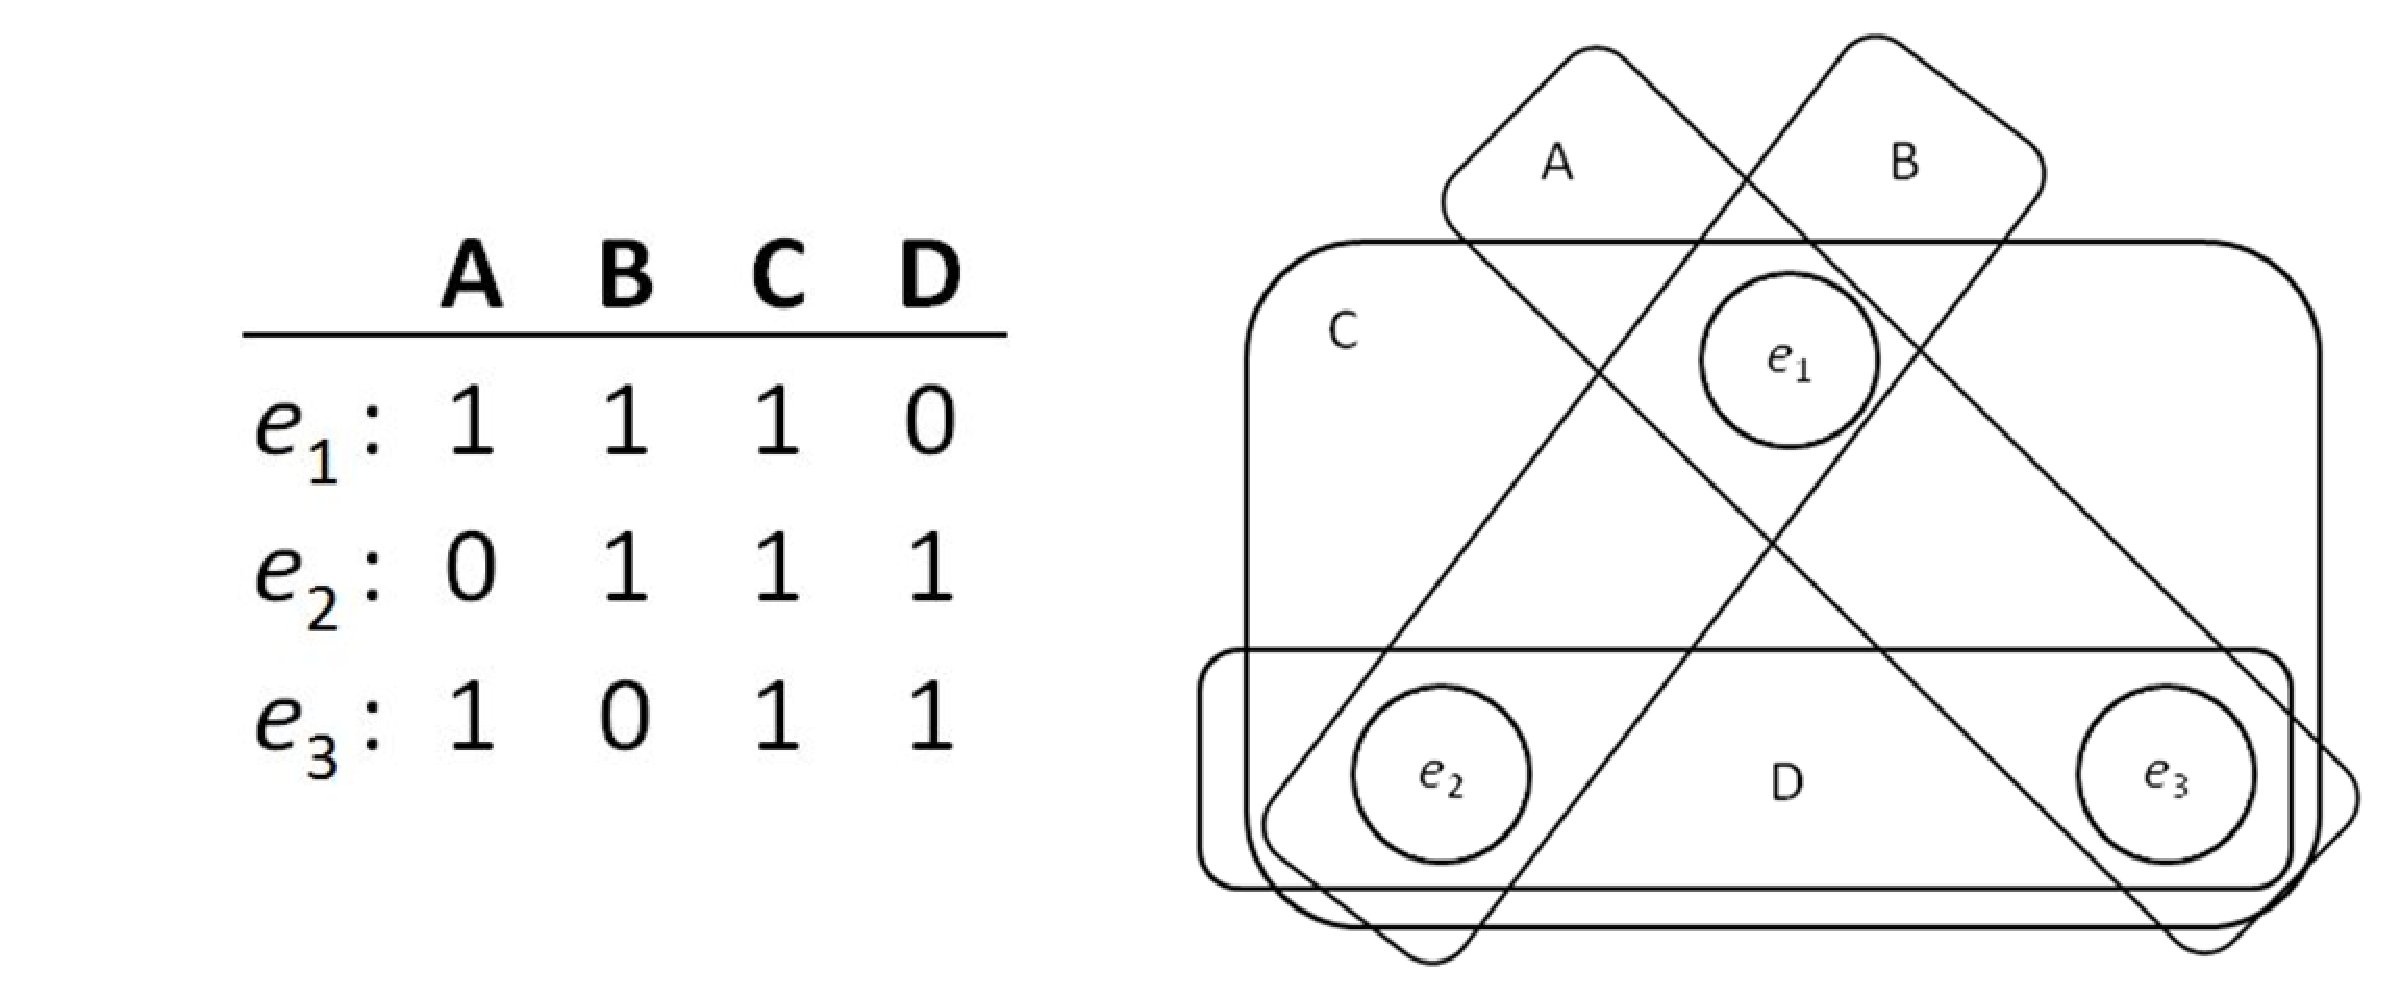
\includegraphics[width=.6\textwidth]{fig/hypergraph-column-wise.eps}
\caption{\label{fig:hypergraph-column-wise} .}
\end{figure}

In Figure.~\ref{fig:hypergraph-column-wise} we show the same motivating example as in Section~\ref{sec:assoc_noonto}. Instead of creating a hyperedge for each row, we create one for each column. A row node is incident on the corresponding hyperedge if it has a value `1' in that column.

%With this hypergraph model, finding semantically associated items amounts to developing a meaningful similarity measure between the items which takes into account the effect of linking items. Such similarity measure should satisfy the intuition that the more ``short" connections between two given items (through linking items), the more similar those items are. To this end, we propose to employ the following quantities as the candidate similarity measure since both of them have the desired property. They are, namely, the \emph{commute time distance} based similarity measure from the random walk model on hypergraph, and the inner product similarity based on the \emph{pseudoinverse of the hypergraph Laplacian}. If the similarity of a pair of items measured by these quantities exceeds some threshold, then this pair of items can be deemed as a semantically associated 2-itemset. Given 2-itemsets, we propose a hypergraph expansion methods based on pruning of its primal graph together with two search strategies in the resulting graph to discover semantically associated $k$-itemsets ($k > 2$).
\subsubsection{Partition-based Clustering}
Given a set of data points $x_1, \ldots x_n$ and some notion of similarity $s(i,j) > 0$ between all pairs of data points $x_i$ and $x_j$ , the common definition of clustering is to divide the data points into several groups such that points in the same group are similar to each other than ones taken from other groups. The relationships among $n$ data points can be specified by means of an $n \times n$ similarity matrix, whose elements $s_{ij}$ measure the similarity of data points $x_i$ and $x_j$.

Partitional clustering algorithms obtain a single partition of the data that optimizes a certain criterion. The most widely used criterion is minimizing the overall squared distance between each data point and the center of its related cluster.

\begin{equation}
argmax_s\sum^k_{i=1}\sum_{x_j\in S}s(j,u_i)^2~, \label{eq:kmeans}
\end{equation}
where $u_i$ is the mean of points in $S_i$. If we restrict the centroids to members of the data, i.e., $u_i \in S_i$, the resulting clustering algorithm is called $k$-medoids algorithm. The optimization problem in Equation~\ref{eq:kmeans} itself is known to be NP-hard, and thus the common approach is to search only for approximate solutions. A particularly well known approximative method is Lloyd's algorithm~\cite{Lloyd83}.

There are several graph-based similarity measures that can be used in the partitional clustering algorithms. The shortest path distance on a graph (also known as the geodesic distance) can be used as the most straight forward measure.
The hypergraph commute time similarity introduced in Section~\ref{sec:assoc_noonto} is more appealing to be used for clustering purposes, because as opposed to the shortest path distance, the commute distance between two vertices decreases if there are many different short ways to get from vertex $v_i$ to vertex $v_j$ . So instead of just looking for the one shortest path, the commute distance looks at the set of short paths. Points which are connected by a short path in the graph and lie in the same high-density region of the graph are considered closer to each other than points which are connected by a short path but lie in different high-density regions of the graph.

To illustrate this point of view, the following example illustrates a comparison between Euclidean distance and commute time distance on a graph shown in Figure~\ref{fig:comm-dist-demo}.



\subsubsection{Spectral Clustering}
If we do not have more information than similarities between data points, a nice way of representing the data is in form of the similarity graph $G = (V,E)$. Each vertex vi in this graph represents a data point $x_i$. Two vertices are connected if the similarity $s_{ij}$ between the corresponding data points $x_i$ and $x_j$ is positive or larger than a certain threshold, and the edge is weighted by $s_{ij}$. The problem of clustering can now be reformulated using the similarity graph: we want to find a partition of the graph such that the edges between different groups have very low weights (which means that points in different clusters are dissimilar from each other) and the edges within a group have high weights (which means that points within the same cluster are similar to each other). To be able to formalize this intuition we first want to introduce some basic graph notation and briefly discuss the kind of graphs we are going to study.

The $\epsilon$-neighborhood graph: Here we connect all points whose pairwise distances are smaller than $\epsilon$. As the distances between all connected points are roughly of the same scale (at most $\epsilon$), weighting the edges would not incorporate more information about the data to the graph. Hence, the $\epsilon$-neighborhood graph is usually considered as an unweighted graph.

$k$-nearest neighbor graphs: Here the goal is to connect vertex $v_i$ with vertex $v_j$ if $v_j$ is among the $k$-nearest neighbors of $v_i$. However, this definition leads to a directed graph, as the neighborhood relationship is not symmetric. There are two ways of making this graph undirected. The first way is to simply ignore the directions of the edges, that is we connect $v_i$ and $v_j$ with an undirected edge if $v_i$ is among the k-nearest neighbors of $v_j$ or if $v_j$ is among the $k$-nearest neighbors of vi. The resulting graph is what is usually called the k-nearest neighbor graph. The second choice is to connect vertices $v_i$ and $v_j$ if both $v_i$ is among the k-nearest neighbors of $v_j$ and $v_j$ is among the $k$-nearest neighbors of $v_i$. The resulting graph is called the mutual $k$-nearest neighbor graph. In both cases, after connecting the appropriate vertices we weight the edges by the similarity of their endpoints.

The fully connected graph: Here we simply connect all points with positive similarity with each other, and we weight all edges by $s_{ij}$ . As the graph should represent the local neighborhood relationships, this construction is only useful if the similarity function itself models local neighborhoods. An example for such a similarity function is the Gaussian similarity function $s(x_i, x_j) = e^{-\|x_i - x_j\|^2/(2\sigma^2)}$, where the parameter $\sigma$ controls the width of the neighborhoods. This parameter plays a similar role as the parameter $\epsilon$ in case of the $\epsilon$-neighborhood graph.


%%%%%%%%%%%%%%%%%%%%%%%%%%%%%%%%%%%%%%%%%%%%%%%%%%%%%%%%%%%%%%%%%%%%%%%%%%%%%%%%%%%%%%%%%%%%%%%%%%%%%%%%%%%%%
\subsection{Classification}
The hypergraph representation for the problem of classification is similar to the one for clustering. We can create hyperedges for columns in the same way as shown in Figure~\ref{fig:hypergraph-column-wise} with the only difference being that a portion of row nodes is labeled and rest unlabeled. The goal for classification is to utilize the information in labeled nodes to come up with correct labels for unlabeled ones.

This problem can be solved by hypergraph-based label propagation. Let $f$ be the objective function (vector) of labels to be learned. Intuitively, there are two criteria for learning the optimal $f$ : (1) we want to assign the same label to vertices that share many incidental hyperedges in common; and (2) assignment of the labels should be similar to the initial labeling $y$. For criteria (1), we define the following cost function
\begin{equation}
\Omega(f,w)=\frac{1}{2}\sum_{e\in E}\sum_{u,v\in e}\frac{w(e)h(u,e)h(v,e)}{d(e)} ~.
\end{equation}
where $I$ is the identity matrix. Here, $D_v$ and $D_e$ are used for computing the normalization of the hypergraph Laplacian, and the unnormalized hypergraph Laplacian is $diag(HD_ew)HWH^T$ . Empirical results showed that the normalized form gives better classification performance for graphbased learning~\cite{Zhou2006}. If the predicted labels on the vertices are consistent with the incidences with the hyperedges, the value of $\Omega(f,w)$ should be minimized. For criteria (2), we directly calculate the squared-loss between the predicted labeling f and the original labeling y as follows,
\begin{equation}
\notag \sum_{u\in V}(f(u)-y(u))^2=\|f-y\|^2
\end{equation}
%%%%%%%%%%%%%%%%%%%%%%%%%%%%%%%%%%%%%%%%%%%%%%%%%%%%%%%%%%%%%%%%%%%%%%%%%%%%%%%%%%%%%%%%%%%%%%%%%%%%%%%%%%%%%

%%%%%%%%%%%%%%%%%%%%%%%%%%%%%%%%%%%%%%%%%%%%%%%%%%%%%%%%%%%%%%%%%%%%
%
%\chapter{CONCLUSION} % and/or future work
%\label{chap:conclusion}
%This dissertation proposes the framework of semantic data mining, a novel direction for the field of data mining that focuses on systematic incorporation of domain knowledge. The enabling technology is based on two contributions presented in the dissertation. First, we develop a graph-based formalism that allows a coherent representation for both the data and the domain knowledge. The key concepts of the approach are bridging the data and the ontology by semantic annotation and employing the RDF bipartite graph as the unified representation. Second, we demonstrate analysis techniques that can be carried out based on the RDF bipartite graph to tackle common data mining tasks, such as the frequent itemset mining, while at the same time leveraging domain knowledge to enhance the performance. For this purpose, several graph-based similarity measures are provided as the key components in the mining algorithms and their trade-offs are studied. The concept of random walk inside the graph while traversing and calculating similarities among nodes are used in designing these measures.

This dissertation also presents the details of some case studies that have validated the hypotheses used in designing the graph-based semantic data mining framework.

\section{Future Work}
Semantic data mining is an emerging field, and many interesting research directions related to it are yet to be explored. The research work presented in this dissertation can be extended in several directions. The following are some of the most important we have identified.

\subsection{Learning Weights Automatically}
The RDF bipartite graph representation relies on the assignment of weights to different types of hyperedges to distinguish the underlying semantics they represent. When ontologies are involved in the mining process, there are at least two types of hyperedges involved, corresponding to RDF statements coming from data and ontologies respectively. Thus at least two different weights have to be assigned with respect to this distinction. In the current work, the (ratio of) weights can be decided purely empirically, or through a series of trial and error experiments on a sampled sub-dataset, which is hardly guaranteed to be accurate or generalizable. Such difficulty is even more noticeable when there are multiple semantic relationships present in the data and ontologies that one hopes to distinguish so as to achieve finer-grained control over their respective contributions to the mining result. Therefore how to automatically derive suitable weights is an important research question.

One technique that can be used is to train a prediction model from labeled data. This approach suffers from the difficulty to acquire the gold-standard training sample. Tian \etal~\cite{Tian2009AHyper} proposed an semi-supervised approach for classifying nodes in a graph based on a relatively small labeled set. The main idea is to formalize the weight assignment and label propagation in one constraint optimization problem while the two objectives can be alternately solved using a two-step iterative method. While this approach is promising, how to extend it to other mining tasks such frequent pattern mining is still an open question.

\subsection{Handling Continuous Features}
The RDF bipartite graph is straightforward to represent binary-valued data and also able to represent nominal-valued data through RDB nominal value expansion. However, there is no immediate solution to make numerical (continuous) data representable. If we enumerate all values present in a numerical feature and create one node in the graph for each of such values, the size of the resulting graph is bound to become intractable. A common way to handle continuous feature is discretization, or binning, as in making histograms. Typical discretization methods include equal interval/frequency partitioning, or more sophisticated ones such as Fayyad and Irani's supervised method called MDL~\cite{FayyadI93discretization} that uses information gain to recursively define the best bins. The more interesting part comes when discretization has to be guided by domain knowledge. For example, certain patterns may make better sense when a column of dates is present and discretized into seasons or quarters rather than arbitrary time intervals. How to represent and execute such domain knowledge in a way that is adaptable to the graph-based semantic data mining framework is a matter of ongoing research. For example the process of domain knowledge guided discretization may hint at a need for a set of rule-based data transformation routines authored under a well-defined protocol that can be treated as a preprocessing step before converting data to graphs. More ways to handle domain knowledge in a standardized way are discussed later in this section.

\subsection{Scalability Issues}
The presented graph-based semantic mining framework heavily relies on the notion of graph-based similarity. We describe the use of several random walk-based measures. The calculation of eigenvectors of the Laplacian is required to derive the similarity measures and is very expensive on large graphs. Non-trivial practical problems are often associated with large scales. For instance, there are more than 30,000 classes in the well-known Gene Ontology, and big online social networks have hundreds of millions of users. Therefore scalability of the graph-based semantic mining methods are of critical importance.

The general solution to is to employ approximation and develop parallelizable algorithms. Lin and Cohen~\cite{LinEtal2010ICML} proposed an approximation to a eigenvalue-weighted linear combination of all the eigenvectors, which can be achieved by performing a small number of matrix-vector multiplications.  Such procedure results in a simple and scalable method called power iteration clustering that finds a very low-dimensional data embedding using truncated power iteration on a normalized pair-wise similarity matrix of the data points. Zhao \etal~\cite{ZhaoEtal2011Eff} described the idea of graph coordinate systems, which embeds graph nodes into points on a coordinate system. By allowing lower distance distortion errors, they were able to develop a practical system that provides fast embedding of large graphs in a hyperbolic space. The embedding algorithm can be parallelized to allow the cost of embedding process being spread across multiple servers. Furthermore, they presented a method to use graph coordinates to efficiently locate shortest paths between node pairs. Such concept can be naturally extended to embed graph nodes according to their commute time distance. Savas and Dhillon~\cite{SavasEtal2011Clu} introduced a novel framework called clustered low rank matrix approximation for massive graphs. The first step is to partition the vertices into a set of disjoint clusters with some fast procedure to preserve important structural information of the original graph. Then a low rank approximation of each cluster is computed independently. Finally the different cluster-wise approximations are combined using an optimal projection step to obtain a low rank approximation of the entire graph, thus including connections or edges between vertices from different clusters. While all these techniques are promising, we will need to extend and them to the RDF bipartite graph and stratification (between data and ontologies and among different semantic types) of the graph may require further adaptions and modifications to those algorithms.

\subsection{New Ways of Representing Complex Domain Semantics}
The RDF bipartite graph can represent concrete semantics such as the ``\emph{is\_a}" or ``\emph{located\_in}" relationship. However meta semantics such as domain/range and cardinality constraints are not so straightforward to be modeled.

One possible approach that can be used to enhance the ability of handling more complex domain semantics in certain applications is to model domain constraints by explicitly describing the desired or acceptable walk (traversal sequence) in the RDF hypergraph. In this case, the recently proposed regular traversal expression ~\cite{Marko10} is worth investigation. In the basic case, we can specify only certain types of nodes in a given random walk. The regular traversal expression can allow us to even specify acceptable path segments or sequences. However, the fast power-iteration approach for computing the stationary probability may not be applicable any more due to the label sequence constraint. To address this problem, we can apply the Monte-Carlo simulation of the random walk to approximate the similarity measure. Note that this approach can be rather scalable as the simulation can be in general constrained in those nodes linking two targeted nodes.

\section{Concluding Remarks}
Although it is widely acknowledged that the use of domain knowledge is important in all stages of the data mining process, research on systematic fusion of the knowledge and data mining still remains in its early stage. Much of the criticisms target the ad hoc manner of the usage of domain knowledge, which causes a tight coupling of assumptions and algorithms and greatly hinders the maintainability and interoperability of mining systems. This situation shows the need to seriously look at different approaches for the incorporation of domain knowledge in addition to attempting to make incremental improvements in existing techniques.

We believe that the designed principles for a graph-based approach for semantic data mining amount to such new approaches for using domain knowledge in a principled manner. As such they should be considered the most important contributions of this dissertation.
%
%%%%%%%%%%%%%%%%%%%%%%%%%%%%%%%%%%%%%%%%%%%%%%%%%%%%%%%%%%%%%%%%%%%%

%APPENDICES
%\appendix
%\include{tappendix_1}

%REFERENCES
\bibliographystyle{unsrtnat}
\bibliography{haishan,thesis}

\end{document} 